\documentclass[twoside,openright,titlepage,numbers=noenddot,headinclude,%
               footinclude=true,cleardoublepage=empty,abstractoff,BCOR=5mm,%
               paper=a4,fontsize=11pt,ngerman,american]{scrreprt}

% ****************************************************************************************************
% classicthesis-config.tex
% formerly known as loadpackages.sty, classicthesis-ldpkg.sty, and classicthesis-preamble.sty
% Use it at the beginning of your ClassicThesis.tex, or as a LaTeX Preamble
% in your ClassicThesis.{tex,lyx} with % ****************************************************************************************************
% classicthesis-config.tex
% formerly known as loadpackages.sty, classicthesis-ldpkg.sty, and classicthesis-preamble.sty
% Use it at the beginning of your ClassicThesis.tex, or as a LaTeX Preamble
% in your ClassicThesis.{tex,lyx} with % ****************************************************************************************************
% classicthesis-config.tex
% formerly known as loadpackages.sty, classicthesis-ldpkg.sty, and classicthesis-preamble.sty
% Use it at the beginning of your ClassicThesis.tex, or as a LaTeX Preamble
% in your ClassicThesis.{tex,lyx} with \input{classicthesis-config}
% ****************************************************************************************************
% If you like the classicthesis, then I would appreciate a postcard.
% My address can be found in the file ClassicThesis.pdf. A collection
% of the postcards I received so far is available online at
% http://postcards.miede.de
% ****************************************************************************************************

% ****************************************************************************************************
% 1. Configure classicthesis for your needs here, e.g., remove "drafting" below
% in order to deactivate the time-stamp on the pages
% ****************************************************************************************************
\PassOptionsToPackage{eulerchapternumbers,listings,drafting,%
				 pdfspacing,eulermath,%floatperchapter,%linedheaders,%
				 subfig,parts}{classicthesis}
% ********************************************************************
% Available options for classicthesis.sty
% (see ClassicThesis.pdf for more information):
% drafting
% parts nochapters linedheaders
% eulerchapternumbers beramono eulermath pdfspacing minionprospacing
% tocaligned dottedtoc manychapters
% listings floatperchapter subfig
% ********************************************************************

% ********************************************************************
% Triggers for this config
% ********************************************************************
\usepackage{ifthen}
\newboolean{enable-backrefs} % enable backrefs in the bibliography
\setboolean{enable-backrefs}{false} % true false
% ****************************************************************************************************


% ****************************************************************************************************
% 2. Personal data and user ad-hoc commands
% ****************************************************************************************************
\newcommand{\myTitle}{Understanding Random Forests\xspace}
\newcommand{\mySubtitle}{From Theory to Practice\xspace}
\newcommand{\myDegree}{Doktor-Ingenieur (Dr.-Ing.)\xspace}
\newcommand{\myName}{Gilles Louppe\xspace}
\newcommand{\myProf}{Put name here\xspace}
\newcommand{\myOtherProf}{Put name here\xspace}
\newcommand{\mySupervisor}{Put name here\xspace}
\newcommand{\myFaculty}{Put data here\xspace}
\newcommand{\myDepartment}{Put data here\xspace}
\newcommand{\myUni}{Put data here\xspace}
\newcommand{\myLocation}{Darmstadt\xspace}
\newcommand{\myTime}{June 2014\xspace}
\newcommand{\myVersion}{version 0.1\xspace}

% ********************************************************************
% Setup, finetuning, and useful commands
% ********************************************************************
\newcounter{dummy} % necessary for correct hyperlinks (to index, bib, etc.)
\newlength{\abcd} % for ab..z string length calculation
\providecommand{\mLyX}{L\kern-.1667em\lower.25em\hbox{Y}\kern-.125emX\@}
\newcommand{\ie}{i.\,e.}
\newcommand{\Ie}{I.\,e.}
\newcommand{\eg}{e.\,g.}
\newcommand{\Eg}{E.\,g.}
% ****************************************************************************************************


% ****************************************************************************************************
% 3. Loading some handy packages
% ****************************************************************************************************
% ********************************************************************
% Packages with options that might require adjustments
% ********************************************************************
\PassOptionsToPackage{latin9}{inputenc}	% latin9 (ISO-8859-9) = latin1+"Euro sign"
 \usepackage{inputenc}

%\PassOptionsToPackage{ngerman,american}{babel}   % change this to your language(s)
% Spanish languages need extra options in order to work with this template
%\PassOptionsToPackage{spanish,es-lcroman}{babel}
 \usepackage{babel}

\PassOptionsToPackage{square,authoryear}{natbib}
 \usepackage{natbib}

\PassOptionsToPackage{fleqn}{amsmath}		% math environments and more by the AMS
 \usepackage{amsmath}

% ********************************************************************
% General useful packages
% ********************************************************************
\PassOptionsToPackage{T1}{fontenc} % T2A for cyrillics
	\usepackage{fontenc}
\usepackage{lipsum}
\usepackage{textcomp} % fix warning with missing font shapes
\usepackage{scrhack} % fix warnings when using KOMA with listings package
\usepackage{xspace} % to get the spacing after macros right
\usepackage{mparhack} % get marginpar right
\usepackage{fixltx2e} % fixes some LaTeX stuff
\PassOptionsToPackage{printonlyused,smaller}{acronym}
	\usepackage{acronym} % nice macros for handling all acronyms in the thesis
%\renewcommand*{\acsfont}[1]{\textssc{#1}} % for MinionPro
\renewcommand{\bflabel}[1]{{#1}\hfill} % fix the list of acronyms
% ****************************************************************************************************


% ****************************************************************************************************
% 4. Setup floats: tables, (sub)figures, and captions
% ****************************************************************************************************
\usepackage{tabularx} % better tables
	\setlength{\extrarowheight}{3pt} % increase table row height
\newcommand{\tableheadline}[1]{\multicolumn{1}{c}{\spacedlowsmallcaps{#1}}}
\newcommand{\myfloatalign}{\centering} % to be used with each float for alignment
\usepackage{caption}
\captionsetup{format=hang,font=small}
\usepackage{subfig}
% ****************************************************************************************************


% ****************************************************************************************************
% 5. Setup code listings
% ****************************************************************************************************
\usepackage{listings}
%\lstset{emph={trueIndex,root},emphstyle=\color{BlueViolet}}%\underbar} % for special keywords
\lstset{language=[LaTeX]Tex,%C++,
    keywordstyle=\color{RoyalBlue},%\bfseries,
    basicstyle=\small\ttfamily,
    %identifierstyle=\color{NavyBlue},
    commentstyle=\color{Green}\ttfamily,
    stringstyle=\rmfamily,
    numbers=none,%left,%
    numberstyle=\scriptsize,%\tiny
    stepnumber=5,
    numbersep=8pt,
    showstringspaces=false,
    breaklines=true,
    frameround=ftff,
    frame=single,
    belowcaptionskip=.75\baselineskip
    %frame=L
}
% ****************************************************************************************************


% ****************************************************************************************************
% 6. PDFLaTeX, hyperreferences and citation backreferences
% ****************************************************************************************************
% ********************************************************************
% Using PDFLaTeX
% ********************************************************************
\PassOptionsToPackage{pdftex,hyperfootnotes=false,pdfpagelabels}{hyperref}
	\usepackage{hyperref}  % backref linktocpage pagebackref
\pdfcompresslevel=9
\pdfadjustspacing=1
\PassOptionsToPackage{pdftex}{graphicx}
	\usepackage{graphicx}

% ********************************************************************
% Setup the style of the backrefs from the bibliography
% (translate the options to any language you use)
% ********************************************************************
\newcommand{\backrefnotcitedstring}{\relax}%(Not cited.)
\newcommand{\backrefcitedsinglestring}[1]{(Cited on page~#1.)}
\newcommand{\backrefcitedmultistring}[1]{(Cited on pages~#1.)}
\ifthenelse{\boolean{enable-backrefs}}%
{%
		\PassOptionsToPackage{hyperpageref}{backref}
		\usepackage{backref} % to be loaded after hyperref package
		   \renewcommand{\backreftwosep}{ and~} % separate 2 pages
		   \renewcommand{\backreflastsep}{, and~} % separate last of longer list
		   \renewcommand*{\backref}[1]{}  % disable standard
		   \renewcommand*{\backrefalt}[4]{% detailed backref
		      \ifcase #1 %
		         \backrefnotcitedstring%
		      \or%
		         \backrefcitedsinglestring{#2}%
		      \else%
		         \backrefcitedmultistring{#2}%
		      \fi}%
}{\relax}

% ********************************************************************
% Hyperreferences
% ********************************************************************
\hypersetup{%
    %draft,	% = no hyperlinking at all (useful in b/w printouts)
    colorlinks=true, linktocpage=true, pdfstartpage=3, pdfstartview=FitV,%
    % uncomment the following line if you want to have black links (e.g., for printing)
    %colorlinks=false, linktocpage=false, pdfborder={0 0 0}, pdfstartpage=3, pdfstartview=FitV,%
    breaklinks=true, pdfpagemode=UseNone, pageanchor=true, pdfpagemode=UseOutlines,%
    plainpages=false, bookmarksnumbered, bookmarksopen=true, bookmarksopenlevel=1,%
    hypertexnames=true, pdfhighlight=/O,%nesting=true,%frenchlinks,%
    urlcolor=webbrown, linkcolor=RoyalBlue, citecolor=webgreen, %pagecolor=RoyalBlue,%
    %urlcolor=Black, linkcolor=Black, citecolor=Black, %pagecolor=Black,%
    pdftitle={\myTitle},%
    pdfauthor={\textcopyright\ \myName, \myUni, \myFaculty},%
    pdfsubject={},%
    pdfkeywords={},%
    pdfcreator={pdfLaTeX},%
    pdfproducer={LaTeX with hyperref and classicthesis}%
}

% ********************************************************************
% Setup autoreferences
% ********************************************************************
% There are some issues regarding autorefnames
% http://www.ureader.de/msg/136221647.aspx
% http://www.tex.ac.uk/cgi-bin/texfaq2html?label=latexwords
% you have to redefine the makros for the
% language you use, e.g., american, ngerman
% (as chosen when loading babel/AtBeginDocument)
% ********************************************************************
\makeatletter
\@ifpackageloaded{babel}%
    {%
       \addto\extrasamerican{%
					\renewcommand*{\figureautorefname}{Figure}%
					\renewcommand*{\tableautorefname}{Table}%
					\renewcommand*{\partautorefname}{Part}%
					\renewcommand*{\chapterautorefname}{Chapter}%
					\renewcommand*{\sectionautorefname}{Section}%
					\renewcommand*{\subsectionautorefname}{Section}%
					\renewcommand*{\subsubsectionautorefname}{Section}%
				}%
       \addto\extrasngerman{%
					\renewcommand*{\paragraphautorefname}{Absatz}%
					\renewcommand*{\subparagraphautorefname}{Unterabsatz}%
					\renewcommand*{\footnoteautorefname}{Fu\"snote}%
					\renewcommand*{\FancyVerbLineautorefname}{Zeile}%
					\renewcommand*{\theoremautorefname}{Theorem}%
					\renewcommand*{\appendixautorefname}{Anhang}%
					\renewcommand*{\equationautorefname}{Gleichung}%
					\renewcommand*{\itemautorefname}{Punkt}%
				}%
			% Fix to getting autorefs for subfigures right (thanks to Belinda Vogt for changing the definition)
			\providecommand{\subfigureautorefname}{\figureautorefname}%
    }{\relax}
\makeatother


% ****************************************************************************************************
% 7. Last calls before the bar closes
% ****************************************************************************************************
% ********************************************************************
% Development Stuff
% ********************************************************************
\listfiles
%\PassOptionsToPackage{l2tabu,orthodox,abort}{nag}
%	\usepackage{nag}
%\PassOptionsToPackage{warning, all}{onlyamsmath}
%	\usepackage{onlyamsmath}

% ********************************************************************
% Last, but not least...
% ********************************************************************
\usepackage{classicthesis}
% ****************************************************************************************************


% ****************************************************************************************************
% 8. Further adjustments (experimental)
% ****************************************************************************************************
% ********************************************************************
% Changing the text area
% ********************************************************************
%\linespread{1.05} % a bit more for Palatino
%\areaset[current]{312pt}{761pt} % 686 (factor 2.2) + 33 head + 42 head \the\footskip
%\setlength{\marginparwidth}{7em}%
%\setlength{\marginparsep}{2em}%

% ********************************************************************
% Using different fonts
% ********************************************************************
%\usepackage[oldstylenums]{kpfonts} % oldstyle notextcomp
%\usepackage[osf]{libertine}
%\usepackage{hfoldsty} % Computer Modern with osf
%\usepackage[light,condensed,math]{iwona}
%\renewcommand{\sfdefault}{iwona}
%\usepackage{lmodern} % <-- no osf support :-(
% \usepackage[T1]{fontenc}
% \usepackage{textcomp}
%\usepackage[urw-garamond]{mathdesign} <-- no osf support :-(
% ****************************************************************************************************

% ****************************************************************************************************
% If you like the classicthesis, then I would appreciate a postcard.
% My address can be found in the file ClassicThesis.pdf. A collection
% of the postcards I received so far is available online at
% http://postcards.miede.de
% ****************************************************************************************************

% ****************************************************************************************************
% 1. Configure classicthesis for your needs here, e.g., remove "drafting" below
% in order to deactivate the time-stamp on the pages
% ****************************************************************************************************
\PassOptionsToPackage{eulerchapternumbers,listings,drafting,%
				 pdfspacing,eulermath,%floatperchapter,%linedheaders,%
				 subfig,parts}{classicthesis}
% ********************************************************************
% Available options for classicthesis.sty
% (see ClassicThesis.pdf for more information):
% drafting
% parts nochapters linedheaders
% eulerchapternumbers beramono eulermath pdfspacing minionprospacing
% tocaligned dottedtoc manychapters
% listings floatperchapter subfig
% ********************************************************************

% ********************************************************************
% Triggers for this config
% ********************************************************************
\usepackage{ifthen}
\newboolean{enable-backrefs} % enable backrefs in the bibliography
\setboolean{enable-backrefs}{false} % true false
% ****************************************************************************************************


% ****************************************************************************************************
% 2. Personal data and user ad-hoc commands
% ****************************************************************************************************
\newcommand{\myTitle}{Understanding Random Forests\xspace}
\newcommand{\mySubtitle}{From Theory to Practice\xspace}
\newcommand{\myDegree}{Doktor-Ingenieur (Dr.-Ing.)\xspace}
\newcommand{\myName}{Gilles Louppe\xspace}
\newcommand{\myProf}{Put name here\xspace}
\newcommand{\myOtherProf}{Put name here\xspace}
\newcommand{\mySupervisor}{Put name here\xspace}
\newcommand{\myFaculty}{Put data here\xspace}
\newcommand{\myDepartment}{Put data here\xspace}
\newcommand{\myUni}{Put data here\xspace}
\newcommand{\myLocation}{Darmstadt\xspace}
\newcommand{\myTime}{June 2014\xspace}
\newcommand{\myVersion}{version 0.1\xspace}

% ********************************************************************
% Setup, finetuning, and useful commands
% ********************************************************************
\newcounter{dummy} % necessary for correct hyperlinks (to index, bib, etc.)
\newlength{\abcd} % for ab..z string length calculation
\providecommand{\mLyX}{L\kern-.1667em\lower.25em\hbox{Y}\kern-.125emX\@}
\newcommand{\ie}{i.\,e.}
\newcommand{\Ie}{I.\,e.}
\newcommand{\eg}{e.\,g.}
\newcommand{\Eg}{E.\,g.}
% ****************************************************************************************************


% ****************************************************************************************************
% 3. Loading some handy packages
% ****************************************************************************************************
% ********************************************************************
% Packages with options that might require adjustments
% ********************************************************************
\PassOptionsToPackage{latin9}{inputenc}	% latin9 (ISO-8859-9) = latin1+"Euro sign"
 \usepackage{inputenc}

%\PassOptionsToPackage{ngerman,american}{babel}   % change this to your language(s)
% Spanish languages need extra options in order to work with this template
%\PassOptionsToPackage{spanish,es-lcroman}{babel}
 \usepackage{babel}

\PassOptionsToPackage{square,authoryear}{natbib}
 \usepackage{natbib}

\PassOptionsToPackage{fleqn}{amsmath}		% math environments and more by the AMS
 \usepackage{amsmath}

% ********************************************************************
% General useful packages
% ********************************************************************
\PassOptionsToPackage{T1}{fontenc} % T2A for cyrillics
	\usepackage{fontenc}
\usepackage{lipsum}
\usepackage{textcomp} % fix warning with missing font shapes
\usepackage{scrhack} % fix warnings when using KOMA with listings package
\usepackage{xspace} % to get the spacing after macros right
\usepackage{mparhack} % get marginpar right
\usepackage{fixltx2e} % fixes some LaTeX stuff
\PassOptionsToPackage{printonlyused,smaller}{acronym}
	\usepackage{acronym} % nice macros for handling all acronyms in the thesis
%\renewcommand*{\acsfont}[1]{\textssc{#1}} % for MinionPro
\renewcommand{\bflabel}[1]{{#1}\hfill} % fix the list of acronyms
% ****************************************************************************************************


% ****************************************************************************************************
% 4. Setup floats: tables, (sub)figures, and captions
% ****************************************************************************************************
\usepackage{tabularx} % better tables
	\setlength{\extrarowheight}{3pt} % increase table row height
\newcommand{\tableheadline}[1]{\multicolumn{1}{c}{\spacedlowsmallcaps{#1}}}
\newcommand{\myfloatalign}{\centering} % to be used with each float for alignment
\usepackage{caption}
\captionsetup{format=hang,font=small}
\usepackage{subfig}
% ****************************************************************************************************


% ****************************************************************************************************
% 5. Setup code listings
% ****************************************************************************************************
\usepackage{listings}
%\lstset{emph={trueIndex,root},emphstyle=\color{BlueViolet}}%\underbar} % for special keywords
\lstset{language=[LaTeX]Tex,%C++,
    keywordstyle=\color{RoyalBlue},%\bfseries,
    basicstyle=\small\ttfamily,
    %identifierstyle=\color{NavyBlue},
    commentstyle=\color{Green}\ttfamily,
    stringstyle=\rmfamily,
    numbers=none,%left,%
    numberstyle=\scriptsize,%\tiny
    stepnumber=5,
    numbersep=8pt,
    showstringspaces=false,
    breaklines=true,
    frameround=ftff,
    frame=single,
    belowcaptionskip=.75\baselineskip
    %frame=L
}
% ****************************************************************************************************


% ****************************************************************************************************
% 6. PDFLaTeX, hyperreferences and citation backreferences
% ****************************************************************************************************
% ********************************************************************
% Using PDFLaTeX
% ********************************************************************
\PassOptionsToPackage{pdftex,hyperfootnotes=false,pdfpagelabels}{hyperref}
	\usepackage{hyperref}  % backref linktocpage pagebackref
\pdfcompresslevel=9
\pdfadjustspacing=1
\PassOptionsToPackage{pdftex}{graphicx}
	\usepackage{graphicx}

% ********************************************************************
% Setup the style of the backrefs from the bibliography
% (translate the options to any language you use)
% ********************************************************************
\newcommand{\backrefnotcitedstring}{\relax}%(Not cited.)
\newcommand{\backrefcitedsinglestring}[1]{(Cited on page~#1.)}
\newcommand{\backrefcitedmultistring}[1]{(Cited on pages~#1.)}
\ifthenelse{\boolean{enable-backrefs}}%
{%
		\PassOptionsToPackage{hyperpageref}{backref}
		\usepackage{backref} % to be loaded after hyperref package
		   \renewcommand{\backreftwosep}{ and~} % separate 2 pages
		   \renewcommand{\backreflastsep}{, and~} % separate last of longer list
		   \renewcommand*{\backref}[1]{}  % disable standard
		   \renewcommand*{\backrefalt}[4]{% detailed backref
		      \ifcase #1 %
		         \backrefnotcitedstring%
		      \or%
		         \backrefcitedsinglestring{#2}%
		      \else%
		         \backrefcitedmultistring{#2}%
		      \fi}%
}{\relax}

% ********************************************************************
% Hyperreferences
% ********************************************************************
\hypersetup{%
    %draft,	% = no hyperlinking at all (useful in b/w printouts)
    colorlinks=true, linktocpage=true, pdfstartpage=3, pdfstartview=FitV,%
    % uncomment the following line if you want to have black links (e.g., for printing)
    %colorlinks=false, linktocpage=false, pdfborder={0 0 0}, pdfstartpage=3, pdfstartview=FitV,%
    breaklinks=true, pdfpagemode=UseNone, pageanchor=true, pdfpagemode=UseOutlines,%
    plainpages=false, bookmarksnumbered, bookmarksopen=true, bookmarksopenlevel=1,%
    hypertexnames=true, pdfhighlight=/O,%nesting=true,%frenchlinks,%
    urlcolor=webbrown, linkcolor=RoyalBlue, citecolor=webgreen, %pagecolor=RoyalBlue,%
    %urlcolor=Black, linkcolor=Black, citecolor=Black, %pagecolor=Black,%
    pdftitle={\myTitle},%
    pdfauthor={\textcopyright\ \myName, \myUni, \myFaculty},%
    pdfsubject={},%
    pdfkeywords={},%
    pdfcreator={pdfLaTeX},%
    pdfproducer={LaTeX with hyperref and classicthesis}%
}

% ********************************************************************
% Setup autoreferences
% ********************************************************************
% There are some issues regarding autorefnames
% http://www.ureader.de/msg/136221647.aspx
% http://www.tex.ac.uk/cgi-bin/texfaq2html?label=latexwords
% you have to redefine the makros for the
% language you use, e.g., american, ngerman
% (as chosen when loading babel/AtBeginDocument)
% ********************************************************************
\makeatletter
\@ifpackageloaded{babel}%
    {%
       \addto\extrasamerican{%
					\renewcommand*{\figureautorefname}{Figure}%
					\renewcommand*{\tableautorefname}{Table}%
					\renewcommand*{\partautorefname}{Part}%
					\renewcommand*{\chapterautorefname}{Chapter}%
					\renewcommand*{\sectionautorefname}{Section}%
					\renewcommand*{\subsectionautorefname}{Section}%
					\renewcommand*{\subsubsectionautorefname}{Section}%
				}%
       \addto\extrasngerman{%
					\renewcommand*{\paragraphautorefname}{Absatz}%
					\renewcommand*{\subparagraphautorefname}{Unterabsatz}%
					\renewcommand*{\footnoteautorefname}{Fu\"snote}%
					\renewcommand*{\FancyVerbLineautorefname}{Zeile}%
					\renewcommand*{\theoremautorefname}{Theorem}%
					\renewcommand*{\appendixautorefname}{Anhang}%
					\renewcommand*{\equationautorefname}{Gleichung}%
					\renewcommand*{\itemautorefname}{Punkt}%
				}%
			% Fix to getting autorefs for subfigures right (thanks to Belinda Vogt for changing the definition)
			\providecommand{\subfigureautorefname}{\figureautorefname}%
    }{\relax}
\makeatother


% ****************************************************************************************************
% 7. Last calls before the bar closes
% ****************************************************************************************************
% ********************************************************************
% Development Stuff
% ********************************************************************
\listfiles
%\PassOptionsToPackage{l2tabu,orthodox,abort}{nag}
%	\usepackage{nag}
%\PassOptionsToPackage{warning, all}{onlyamsmath}
%	\usepackage{onlyamsmath}

% ********************************************************************
% Last, but not least...
% ********************************************************************
\usepackage{classicthesis}
% ****************************************************************************************************


% ****************************************************************************************************
% 8. Further adjustments (experimental)
% ****************************************************************************************************
% ********************************************************************
% Changing the text area
% ********************************************************************
%\linespread{1.05} % a bit more for Palatino
%\areaset[current]{312pt}{761pt} % 686 (factor 2.2) + 33 head + 42 head \the\footskip
%\setlength{\marginparwidth}{7em}%
%\setlength{\marginparsep}{2em}%

% ********************************************************************
% Using different fonts
% ********************************************************************
%\usepackage[oldstylenums]{kpfonts} % oldstyle notextcomp
%\usepackage[osf]{libertine}
%\usepackage{hfoldsty} % Computer Modern with osf
%\usepackage[light,condensed,math]{iwona}
%\renewcommand{\sfdefault}{iwona}
%\usepackage{lmodern} % <-- no osf support :-(
% \usepackage[T1]{fontenc}
% \usepackage{textcomp}
%\usepackage[urw-garamond]{mathdesign} <-- no osf support :-(
% ****************************************************************************************************

% ****************************************************************************************************
% If you like the classicthesis, then I would appreciate a postcard.
% My address can be found in the file ClassicThesis.pdf. A collection
% of the postcards I received so far is available online at
% http://postcards.miede.de
% ****************************************************************************************************

% ****************************************************************************************************
% 1. Configure classicthesis for your needs here, e.g., remove "drafting" below
% in order to deactivate the time-stamp on the pages
% ****************************************************************************************************
\PassOptionsToPackage{eulerchapternumbers,listings,drafting,%
				 pdfspacing,eulermath,%floatperchapter,%linedheaders,%
				 subfig,parts}{classicthesis}
% ********************************************************************
% Available options for classicthesis.sty
% (see ClassicThesis.pdf for more information):
% drafting
% parts nochapters linedheaders
% eulerchapternumbers beramono eulermath pdfspacing minionprospacing
% tocaligned dottedtoc manychapters
% listings floatperchapter subfig
% ********************************************************************

% ********************************************************************
% Triggers for this config
% ********************************************************************
\usepackage{ifthen}
\newboolean{enable-backrefs} % enable backrefs in the bibliography
\setboolean{enable-backrefs}{false} % true false
% ****************************************************************************************************


% ****************************************************************************************************
% 2. Personal data and user ad-hoc commands
% ****************************************************************************************************
\newcommand{\myTitle}{Understanding Random Forests\xspace}
\newcommand{\mySubtitle}{From Theory to Practice\xspace}
\newcommand{\myDegree}{Doktor-Ingenieur (Dr.-Ing.)\xspace}
\newcommand{\myName}{Gilles Louppe\xspace}
\newcommand{\myProf}{Put name here\xspace}
\newcommand{\myOtherProf}{Put name here\xspace}
\newcommand{\mySupervisor}{Put name here\xspace}
\newcommand{\myFaculty}{Put data here\xspace}
\newcommand{\myDepartment}{Put data here\xspace}
\newcommand{\myUni}{Put data here\xspace}
\newcommand{\myLocation}{Darmstadt\xspace}
\newcommand{\myTime}{June 2014\xspace}
\newcommand{\myVersion}{version 0.1\xspace}

% ********************************************************************
% Setup, finetuning, and useful commands
% ********************************************************************
\newcounter{dummy} % necessary for correct hyperlinks (to index, bib, etc.)
\newlength{\abcd} % for ab..z string length calculation
\providecommand{\mLyX}{L\kern-.1667em\lower.25em\hbox{Y}\kern-.125emX\@}
\newcommand{\ie}{i.\,e.}
\newcommand{\Ie}{I.\,e.}
\newcommand{\eg}{e.\,g.}
\newcommand{\Eg}{E.\,g.}
% ****************************************************************************************************


% ****************************************************************************************************
% 3. Loading some handy packages
% ****************************************************************************************************
% ********************************************************************
% Packages with options that might require adjustments
% ********************************************************************
\PassOptionsToPackage{latin9}{inputenc}	% latin9 (ISO-8859-9) = latin1+"Euro sign"
 \usepackage{inputenc}

%\PassOptionsToPackage{ngerman,american}{babel}   % change this to your language(s)
% Spanish languages need extra options in order to work with this template
%\PassOptionsToPackage{spanish,es-lcroman}{babel}
 \usepackage{babel}

\PassOptionsToPackage{square,authoryear}{natbib}
 \usepackage{natbib}

\PassOptionsToPackage{fleqn}{amsmath}		% math environments and more by the AMS
 \usepackage{amsmath}

% ********************************************************************
% General useful packages
% ********************************************************************
\PassOptionsToPackage{T1}{fontenc} % T2A for cyrillics
	\usepackage{fontenc}
\usepackage{lipsum}
\usepackage{textcomp} % fix warning with missing font shapes
\usepackage{scrhack} % fix warnings when using KOMA with listings package
\usepackage{xspace} % to get the spacing after macros right
\usepackage{mparhack} % get marginpar right
\usepackage{fixltx2e} % fixes some LaTeX stuff
\PassOptionsToPackage{printonlyused,smaller}{acronym}
	\usepackage{acronym} % nice macros for handling all acronyms in the thesis
%\renewcommand*{\acsfont}[1]{\textssc{#1}} % for MinionPro
\renewcommand{\bflabel}[1]{{#1}\hfill} % fix the list of acronyms
% ****************************************************************************************************


% ****************************************************************************************************
% 4. Setup floats: tables, (sub)figures, and captions
% ****************************************************************************************************
\usepackage{tabularx} % better tables
	\setlength{\extrarowheight}{3pt} % increase table row height
\newcommand{\tableheadline}[1]{\multicolumn{1}{c}{\spacedlowsmallcaps{#1}}}
\newcommand{\myfloatalign}{\centering} % to be used with each float for alignment
\usepackage{caption}
\captionsetup{format=hang,font=small}
\usepackage{subfig}
% ****************************************************************************************************


% ****************************************************************************************************
% 5. Setup code listings
% ****************************************************************************************************
\usepackage{listings}
%\lstset{emph={trueIndex,root},emphstyle=\color{BlueViolet}}%\underbar} % for special keywords
\lstset{language=[LaTeX]Tex,%C++,
    keywordstyle=\color{RoyalBlue},%\bfseries,
    basicstyle=\small\ttfamily,
    %identifierstyle=\color{NavyBlue},
    commentstyle=\color{Green}\ttfamily,
    stringstyle=\rmfamily,
    numbers=none,%left,%
    numberstyle=\scriptsize,%\tiny
    stepnumber=5,
    numbersep=8pt,
    showstringspaces=false,
    breaklines=true,
    frameround=ftff,
    frame=single,
    belowcaptionskip=.75\baselineskip
    %frame=L
}
% ****************************************************************************************************


% ****************************************************************************************************
% 6. PDFLaTeX, hyperreferences and citation backreferences
% ****************************************************************************************************
% ********************************************************************
% Using PDFLaTeX
% ********************************************************************
\PassOptionsToPackage{pdftex,hyperfootnotes=false,pdfpagelabels}{hyperref}
	\usepackage{hyperref}  % backref linktocpage pagebackref
\pdfcompresslevel=9
\pdfadjustspacing=1
\PassOptionsToPackage{pdftex}{graphicx}
	\usepackage{graphicx}

% ********************************************************************
% Setup the style of the backrefs from the bibliography
% (translate the options to any language you use)
% ********************************************************************
\newcommand{\backrefnotcitedstring}{\relax}%(Not cited.)
\newcommand{\backrefcitedsinglestring}[1]{(Cited on page~#1.)}
\newcommand{\backrefcitedmultistring}[1]{(Cited on pages~#1.)}
\ifthenelse{\boolean{enable-backrefs}}%
{%
		\PassOptionsToPackage{hyperpageref}{backref}
		\usepackage{backref} % to be loaded after hyperref package
		   \renewcommand{\backreftwosep}{ and~} % separate 2 pages
		   \renewcommand{\backreflastsep}{, and~} % separate last of longer list
		   \renewcommand*{\backref}[1]{}  % disable standard
		   \renewcommand*{\backrefalt}[4]{% detailed backref
		      \ifcase #1 %
		         \backrefnotcitedstring%
		      \or%
		         \backrefcitedsinglestring{#2}%
		      \else%
		         \backrefcitedmultistring{#2}%
		      \fi}%
}{\relax}

% ********************************************************************
% Hyperreferences
% ********************************************************************
\hypersetup{%
    %draft,	% = no hyperlinking at all (useful in b/w printouts)
    colorlinks=true, linktocpage=true, pdfstartpage=3, pdfstartview=FitV,%
    % uncomment the following line if you want to have black links (e.g., for printing)
    %colorlinks=false, linktocpage=false, pdfborder={0 0 0}, pdfstartpage=3, pdfstartview=FitV,%
    breaklinks=true, pdfpagemode=UseNone, pageanchor=true, pdfpagemode=UseOutlines,%
    plainpages=false, bookmarksnumbered, bookmarksopen=true, bookmarksopenlevel=1,%
    hypertexnames=true, pdfhighlight=/O,%nesting=true,%frenchlinks,%
    urlcolor=webbrown, linkcolor=RoyalBlue, citecolor=webgreen, %pagecolor=RoyalBlue,%
    %urlcolor=Black, linkcolor=Black, citecolor=Black, %pagecolor=Black,%
    pdftitle={\myTitle},%
    pdfauthor={\textcopyright\ \myName, \myUni, \myFaculty},%
    pdfsubject={},%
    pdfkeywords={},%
    pdfcreator={pdfLaTeX},%
    pdfproducer={LaTeX with hyperref and classicthesis}%
}

% ********************************************************************
% Setup autoreferences
% ********************************************************************
% There are some issues regarding autorefnames
% http://www.ureader.de/msg/136221647.aspx
% http://www.tex.ac.uk/cgi-bin/texfaq2html?label=latexwords
% you have to redefine the makros for the
% language you use, e.g., american, ngerman
% (as chosen when loading babel/AtBeginDocument)
% ********************************************************************
\makeatletter
\@ifpackageloaded{babel}%
    {%
       \addto\extrasamerican{%
					\renewcommand*{\figureautorefname}{Figure}%
					\renewcommand*{\tableautorefname}{Table}%
					\renewcommand*{\partautorefname}{Part}%
					\renewcommand*{\chapterautorefname}{Chapter}%
					\renewcommand*{\sectionautorefname}{Section}%
					\renewcommand*{\subsectionautorefname}{Section}%
					\renewcommand*{\subsubsectionautorefname}{Section}%
				}%
       \addto\extrasngerman{%
					\renewcommand*{\paragraphautorefname}{Absatz}%
					\renewcommand*{\subparagraphautorefname}{Unterabsatz}%
					\renewcommand*{\footnoteautorefname}{Fu\"snote}%
					\renewcommand*{\FancyVerbLineautorefname}{Zeile}%
					\renewcommand*{\theoremautorefname}{Theorem}%
					\renewcommand*{\appendixautorefname}{Anhang}%
					\renewcommand*{\equationautorefname}{Gleichung}%
					\renewcommand*{\itemautorefname}{Punkt}%
				}%
			% Fix to getting autorefs for subfigures right (thanks to Belinda Vogt for changing the definition)
			\providecommand{\subfigureautorefname}{\figureautorefname}%
    }{\relax}
\makeatother


% ****************************************************************************************************
% 7. Last calls before the bar closes
% ****************************************************************************************************
% ********************************************************************
% Development Stuff
% ********************************************************************
\listfiles
%\PassOptionsToPackage{l2tabu,orthodox,abort}{nag}
%	\usepackage{nag}
%\PassOptionsToPackage{warning, all}{onlyamsmath}
%	\usepackage{onlyamsmath}

% ********************************************************************
% Last, but not least...
% ********************************************************************
\usepackage{classicthesis}
% ****************************************************************************************************


% ****************************************************************************************************
% 8. Further adjustments (experimental)
% ****************************************************************************************************
% ********************************************************************
% Changing the text area
% ********************************************************************
%\linespread{1.05} % a bit more for Palatino
%\areaset[current]{312pt}{761pt} % 686 (factor 2.2) + 33 head + 42 head \the\footskip
%\setlength{\marginparwidth}{7em}%
%\setlength{\marginparsep}{2em}%

% ********************************************************************
% Using different fonts
% ********************************************************************
%\usepackage[oldstylenums]{kpfonts} % oldstyle notextcomp
%\usepackage[osf]{libertine}
%\usepackage{hfoldsty} % Computer Modern with osf
%\usepackage[light,condensed,math]{iwona}
%\renewcommand{\sfdefault}{iwona}
%\usepackage{lmodern} % <-- no osf support :-(
% \usepackage[T1]{fontenc}
% \usepackage{textcomp}
%\usepackage[urw-garamond]{mathdesign} <-- no osf support :-(
% ****************************************************************************************************


\usepackage{amsthm}
\newtheorem{theorem}{Theorem}
\newtheorem{lemma}[theorem]{Lemma}
\newtheorem{proposition}[theorem]{Proposition}
\newtheorem{corollary}[theorem]{Corollary}
\newtheorem{definition}{Definition}

\newcommand{\todo}[1]{\textcolor{red}{\textit{[TODO] #1}}}

\begin{document}
\frenchspacing
\raggedbottom
\selectlanguage{american}
\pagenumbering{roman}
\pagestyle{plain}

% Front pages =================================================================
% Front page ==================================================================

\begin{titlepage}
	\begin{addmargin}[-1cm]{-3cm}
    \begin{center}
        \large

        \hfill
        \vfill

        \begingroup
            \color{Maroon}\spacedallcaps{\myTitle} \\ \bigskip
        \endgroup

        \spacedlowsmallcaps{\myName}

        \vfill
    \end{center}
  \end{addmargin}
\end{titlepage}

\cleardoublepage% Abstract ====================================================================

\pdfbookmark[1]{Abstract}{Abstract}
\chapter*{Abstract}

Data analysis and machine learning have become an integrative part of the
modern scientific methodology, offering automated procedures for the prediction
of a phenomenon based on past observations, unraveling underlying patterns in
data and providing insights about the problem. Yet, caution should
avoid using machine learning as a black-box tool, but rather consider it as a
methodology, with a rational thought process that is entirely dependent on the
problem under study. In particular, the use of algorithms
should ideally require a reasonable understanding of their
mechanisms, properties and limitations, in order to better apprehend and
interpret their results.

The goal of this dissertation is to provide an in-depth
analysis of random forests, consistently calling into
question each and every part of the algorithm, in order to shed new light on
its learning capabilities, inner workings and interpretability. The first
part of this work studies the induction of decision trees and the construction of
ensemble of randomized trees, motivating their design and purpose whenever
possible. Our contributions follow with an original complexity
analysis of random forests, hence showing their good computational performance
and scalability, along with an in-depth discussion of their
implementation details, as contributed within Scikit-Learn.

In the second part of this work, we analyze and discuss the interpretability of
random forests in the eyes of variable importances measures. The core of our
contributions rests in the theoretical characterization of the Mean Decrease of
Impurity variable importance measure, from which we prove and derive some of
its properties in the case of multiway totally randomized trees and in
asymptotic conditions. In consequence of this work, our analysis  demonstrates
that variable importances as computed from non-totally randomized trees (e.g.,
standard Random Forest) suffer from a combination of defects, due to masking
effects, misestimations of node impurity or due to the binary structure of
decision trees.

Finally, the last part of this thesis addresses limitations of random forests
in the context of large datasets. Through extensive experiments, we show
that subsampling both samples and features simultaneously provides on
par performance while lowering at the same time the memory requirements.
Overall this paradigm highlights an intriguing practical fact: there is often
no need to build single models over immensely large datasets. Good performance
can often be achieved by building models on (very) small random parts of the
data and then combining them all in an ensemble, thereby avoiding all practical burdens of making large data fit into memory.

\cleardoublepage%*******************************************************
% Publications
%*******************************************************
\pdfbookmark[1]{Publications}{publications}
\chapter*{Publications}
Some ideas and figures have appeared previously in the following publications:

\bigskip

\noindent Put your publications from the thesis here. The packages \texttt{multibib} or \texttt{bibtopic} etc. can be used to handle multiple different bibliographies in your document.
\cleardoublepage%*******************************************************
% Acknowledgments
%*******************************************************
\pdfbookmark[1]{Acknowledgments}{acknowledgments}

\begin{flushright}{\slshape    
    We have seen that computer programming is an art, \\ 
    because it applies accumulated knowledge to the world, \\ 
    because it requires skill and ingenuity, and especially \\
    because it produces objects of beauty.} \\ \medskip
    --- \defcitealias{knuth:1974}{Donald E. Knuth}\citetalias{knuth:1974} \citep{knuth:1974}
\end{flushright}



\bigskip

\begingroup
\let\clearpage\relax
\let\cleardoublepage\relax
\let\cleardoublepage\relax
\chapter*{Acknowledgments}
Put your acknowledgments here.

Many thanks to everybody who already sent me a postcard!

Regarding the typography and other help, many thanks go to Marco 
Kuhlmann, Philipp Lehman, Lothar Schlesier, Jim Young, Lorenzo 
Pantieri and Enrico Gregorio\footnote{Members of GuIT (Gruppo 
Italiano Utilizzatori di \TeX\ e \LaTeX )}, J\"org Sommer, 
Joachim K\"ostler, Daniel Gottschlag, Denis Aydin, Paride 
Legovini, Steffen Prochnow, Nicolas Repp, Hinrich Harms, 
 Roland Winkler, J\"org Weber, 
 and the whole \LaTeX-community for support, ideas and 
 some great software.

\bigskip

\noindent\emph{Regarding \mLyX}: The \mLyX\ port was intially done by 
\emph{Nicholas Mariette} in March 2009 and continued by 
\emph{Ivo Pletikosi\'c} in 2011. Thank you very much for your 
work and the contributions to the original style.


\endgroup




\pagestyle{scrheadings}
\cleardoublepage%*******************************************************
% Table of Contents
%*******************************************************
%\phantomsection
\refstepcounter{dummy}
\pdfbookmark[1]{\contentsname}{tableofcontents}
\setcounter{tocdepth}{2} % <-- 2 includes up to subsections in the ToC
\setcounter{secnumdepth}{3} % <-- 3 numbers up to subsubsections
\manualmark
\markboth{\spacedlowsmallcaps{\contentsname}}{\spacedlowsmallcaps{\contentsname}}
\tableofcontents 
\automark[section]{chapter}
\renewcommand{\chaptermark}[1]{\markboth{\spacedlowsmallcaps{#1}}{\spacedlowsmallcaps{#1}}}
\renewcommand{\sectionmark}[1]{\markright{\thesection\enspace\spacedlowsmallcaps{#1}}}
%*******************************************************
% List of Figures and of the Tables
%*******************************************************
\clearpage

\begingroup 
    \let\clearpage\relax
    \let\cleardoublepage\relax
    \let\cleardoublepage\relax
    %*******************************************************
    % List of Figures
    %*******************************************************    
    %\phantomsection 
    \refstepcounter{dummy}
    %\addcontentsline{toc}{chapter}{\listfigurename}
    \pdfbookmark[1]{\listfigurename}{lof}
    \listoffigures

    \vspace*{8ex}

    %*******************************************************
    % List of Tables
    %*******************************************************
    %\phantomsection 
    \refstepcounter{dummy}
    %\addcontentsline{toc}{chapter}{\listtablename}
    \pdfbookmark[1]{\listtablename}{lot}
    \listoftables
        
    \vspace*{8ex}
%   \newpage
    
    %*******************************************************
    % List of Listings
    %*******************************************************      
	  %\phantomsection 
    \refstepcounter{dummy}
    %\addcontentsline{toc}{chapter}{\lstlistlistingname}
    \pdfbookmark[1]{\lstlistlistingname}{lol}
    \lstlistoflistings 

    \vspace*{8ex}
       
    %*******************************************************
    % Acronyms
    %*******************************************************
    %\phantomsection 
    \refstepcounter{dummy}
    \pdfbookmark[1]{Acronyms}{acronyms}
    \markboth{\spacedlowsmallcaps{Acronyms}}{\spacedlowsmallcaps{Acronyms}}
    \chapter*{Acronyms}
    \begin{acronym}[UML]
        \acro{DRY}{Don't Repeat Yourself}
        \acro{API}{Application Programming Interface}
        \acro{UML}{Unified Modeling Language}
    \end{acronym}                     
\endgroup

\cleardoublepage


% Content =====================================================================
\pagenumbering{arabic}

\cleardoublepage
\chapter{Introduction}\label{ch:introduction}

In various fields of science and technology, like in medicine, psychology,
meteorology, finance or robotics to cite a few, experts aim at predicting a
phenomenon based on past observations or measurements. For instance,
meteorologists try to forecast the weather for the next days from the climatic
conditions of the previous days. In medicine, practicians collect measurements
and information such as blood pressure, age or history for diagnosing the
condition of incoming patients. Similarly, in chemistry, compounds are analyzed
using mass spectrometry measurements in order to determine whether they contain
a given type of molecules or atoms. In all of these cases, the goal is
the prediction of a response variable based on a set of predictor
variables.

For centuries, scientists have addressed these questions by deriving
theoretical frameworks from first principles or have accumulated knowledge in
order to model, analyze and understand the pheno\-menon under study. For
example, practicians know from past experience that elderly heart attack
patients with low blood pressure are generally high risk. Similarly,
meteorologists know from elementary climate models that one hot, high pollution
day is likely to be followed by another. For an increasing number of problems
however, standard approaches start showing their limits. Identifying the
genetic risk factors for heart disease for example, where knowledge is still
very sparse, is nearly impractical for the cognitive abilities of humans given
the high complexity and intricacy of interactions that exist between genes.
Likewise, for very fine-grained meteorological forecasts, a large number of
variables need to be taken into account, which quickly goes beyond the
capabilities of experts to put them all into a unified set equations. To break
this cognitive barrier and further advance science, machines of increasing
speed and capacity have been built and designed since the mid-twentieth century
to assist humans in their calculations. However, alongside this progress in
terms of hardware, developments in theoretical computer science, artificial
intelligence and statistics have made machines to become more than calculators.
Recent advances have made them experts of their own kind, capable to learn from
data and to uncover by themselves the predictive structure of problems.
Techniques and algorithms that have stemmed from the field of {\it machine
learning} have now become a powerful tool for the analysis of complex and large
data, successfully assisting scientists in numerous breakthroughs of various
fields of science and technology.

Formally, machine learning can be defined as the study of systems that can
learn from data without being explicitely programmed. According to
\citet{mitchell:1997}, a computer program is said to learn from data, with
respect to some class of task and performance measure if its performance at
thoses tasks improves with data. In particular, machine learning provide
algorithms that are able to solve classification or regression tasks, hence
yielding now automated procedures for the prediction of a phenomenon based on
past observations. However, the goal of machine learning is not only to produce
algorithms making accurate predictions, it is also to provide insight and
undestanding into the predictive structure of the data~\citep{breiman:1984}.



% ==> In plain English (no maths!)
% General introduction to ML
%  => pourquoi se passer de l'humain et désirer qu'une machine apprenne? (Zighed pg 20)
% Goals and purposes of ML, examples of applications
% => interprétabilité, extraction de connaissances à partir de données
% Tree-based methods (introduction, atouts, etc)
% Content of the thesis

% Reuse content from tentative paper




\cleardoublepage
%\ctparttex{}
\part{Growing Decision Trees}\label{part:1}
\chapter{Background}\label{ch:background}

\section{Learning from data}

In the examples introduced in Chapter~\ref{ch:introduction}, the objective
which is sought is to find a systematic way of predicting a phenomenon given a
set of measurements. In machine learning terms, this goal is formulated as the
{\it supervised learning} task of infering from collected data a model that
predicts the value of an output variable based on the observed values of input
variables. As such, finding an appropriate model is based on the assumption
that the output variable does not take its value at random and that there
exists a relation between the inputs and the output. In medicine for instance,
the goal is to find a decision rule (i.e., a model) from a set of past cases
(i.e., the collected data) for predicting the condition of an incoming patient
(i.e., the output value) given a set of measurements such as age, sex, blood
pressure or history (i.e., the input values).

To give a more precise formulation, let us arrange the set of measurements on a
case in a pre-assigned order, i.e., take the input values to be $x_1, x_2, ...,
x_p$, where $x_j \in {\cal X}_j$ (for $j = 1, ..., p$) corresponds to the value
of the input variable $X_j$. Together, the input values $(x_1, x_2, ..., x_p)$
form a $p$-dimensional input vector $\mathbf{x}$ taking its values in ${\cal
X}_1 \times ... \times {\cal X}_p = {\cal X}$, where ${\cal X}$ is defined as
the input space. Similarly, let us define as $y \in {\cal Y}$ the value of the
output variable $Y$, where ${\cal Y}$ is defined as the output
space\footnote{Unless stated otherwise, supervised learning is reduced to the
prediction of a \textit{single} output variable. More generally however, this
framework can be defined as the prediction of one or several output variables.}.
By definition, both the input and the output spaces are assumed to respectively
contain all possible input vectors and all possible output values. Note that
input variables are sometimes known as {\it features}, input vectors as {\it
objects}, {\it examples} or {\it samples} and the output variable as {\it
target}.

Among variables that define the problem, we distinguish between two general
types. The former correspond to quantitative variables whose values are integer
or real numbers, such as age or blood pressure. The latter correspond to
qualitative variables whose values are symbolic, such as gender or condition.
Formally, we define them as follows:

\begin{definition}
A variable $X_j$ is \emph{numerical} or \emph{ordered} if ${\cal X}_j$ is a
totally ordered set.
\end{definition}

\begin{definition}
A variable $X_j$ is \emph{categorical} if ${\cal X}_j$ is a finite set of values,
without any natural order.
\end{definition}

In a typical supervised learning task, past observations are summarized by a
dataset called {\it learning set}. It consists in a set of observed input
vectors together with their actual output value and formally defined as
follows:

\begin{definition}
A \emph{learning set} ${\cal L}$ is a set of $N$
pairs of input vectors and output values $(\mathbf{x}_1, y_1), ...,
(\mathbf{x}_N, y_N)$, where $\mathbf{x}_i \in {\cal X}$ and $y_i \in {\cal Y}$.
\end{definition}

Equivalently, a set of $p$-input vectors $\mathbf{x}_i$ (for $i=1, ..., N$) can
be denoted by a $N\times p$ matrix $\mathbf{X}$, whose rows $i=1, ..., N$
correspond to input vectors $\mathbf{x}_i$ and columns $j=1, ..., p$ to input
variables $X_j$. Similarly, the corresponding output values can be written as a
vector $\mathbf{y}=(y_1, ..., y_N)$.

\begin{remark}{Data representation}
For optimal implementations of machine learning algorithms, data needs to
represented using structures which allows for high-performance numerical
computation. In this work, code snippets are described under  that assumption
that data is represented using a data structure similar to a NumPy
array~\citep{vanderwalt:2011}.

A NumPy array is basically a multidimensional uniform collection of values, all
of the same type and organized in a given shape. For instance, a matrix
$\mathbf{X}$ can be represented as a 2-dimensional NumPy array of shape $N
\times p$ that contains numbers (e.g., floating point values or integers). This
structure allows for random access in constant time, vectorized high-level
operations and efficient memory usage.

Additionally, using a data representation which is close to the matrix
formulation, like NumPy arrays, makes it possible to write implementations that
are close to their original textbook formulation, thereby making them easier to
understand and maintain. \end{remark}

In this framework, the supervised learning task can be stated as learning a
function $\varphi: {\cal X} \mapsto {\cal Y}$ from a learning set ${\cal
L}=(\mathbf{X}, \mathbf{y})$. In particular, the goal of the learning task is
to find a model such that its predictions $\varphi(\mathbf{x})$, also denoted
by the variable $\hat{Y}$, are as good as possible. If $Y$ is a categorical
variable then the learning task is a classification problem. If $Y$ is
numerical variable, then learning task is a regression problem. Without loss of
generality, the resulting models can be defined as
follows:

\begin{definition}
A \emph{classifier} or \emph{classification rule} is a function $\varphi: {\cal X}
\mapsto {\cal Y}$, where ${\cal Y}$ is a finite set of classes denoted $\{1, 2, ..., J\}$.
\end{definition}

\begin{definition}
A \emph{regressor} is a function $\varphi: {\cal X} \mapsto {\cal Y}$, where ${\cal Y}=\mathbb{R}$.
\end{definition}

\begin{remark}{Estimator interface}
We follow in this work the API conventions proposed by~\citet{buitinck:2013}.
In particular, learning algorithms are described as \textit{estimator} objects implementing the
following interface:

\begin{itemize}
\item[-] Hyper-parameters of an algorithm are all passed to the constructor of the
estimator. The constructor does not see any actual data. All it does
is to attach hyper-parameters values as public attributes to the estimator object.
\item[-] Learning is performed in a \texttt{fit} method. This method is called with
a learning set (e.g., supplied as two arrays \texttt{X\_train} and \texttt{y\_train}). Its
task is to run a learning algorithm and to determine model-specific parameters
from the data. The \texttt{fit} method always returns the estimator object
it was called on, which now serves as a model and can be used to make predictions.
\item[-] Predictions are performed through a \texttt{predict} method, taking
as input an array \texttt{X\_test} and producing as output the predictions for
\texttt{X\_test} based on the learned parameters. In the case of classification,
this method returns labels from ${\cal Y} = \{1, 2, ..., J\}$. In the case of regression,
it returns numerical values from ${\cal Y} = \mathbb{R}$.
\end{itemize}

With this API, a typical supervised learning task is performed as follows:

\vskip0.3cm
\begin{pythoncode}
# Instantiate and set hyper-parameters
clf = DecisionTreeClassifier(max_depth=5)
# Learn a model from data
clf.fit(X_train, y_train)
# Make predictions on new data
y_hat = clf.predict(X_test)
\end{pythoncode}
\end{remark}


\section{Performance evaluation}

In the statistical sense, input and output variables $X_1, ..., X_p$ and $Y$
are \textit{random variables} taking jointly their values from ${\cal X}
\times {\cal Y}$ with respect to the joint probability distribution $P(X, Y)$,
where $X$ denotes the random vector $(X_1, ..., X_p)$. That is,
$P(X=\mathbf{x}, Y=y)$ is the probability of drawing the couple $(\mathbf{x},
y)$ at random from ${\cal X} \times {\cal Y}$.

Accordingly, learning  a model $\varphi$ whose predictions are as good as
possible can be stated as finding a model $\varphi$ which minimizes its
expected prediction error, defined as follows:

\begin{definition}
The \emph{expected prediction error}, also known as \emph{generalization
error} or \emph{test error}, of the model $\varphi$ is\footnote{$\mathbb{E}_X \{f(X)\}$ denotes the expected value of $f(x)$
(for $x \in {\cal X}$) with respect to the probability distribution of the
random variable $X$. It is defined as $$\mathbb{E}_X \{f(X)\} = \sum_{x \in {\cal
X}} P(X=x) f(x).$$}
\begin{equation}\label{eqn:generalization-error}
Err_{{\cal L}}(\varphi) = \mathbb{E}_{X, Y}\{ L(Y, \varphi(X)) | {\cal L} \},
\end{equation}
where ${\cal L}$ is the learning set used to build $\varphi$ and $L$ is a loss
function measuring the discrepancy between its two
arguments~\citep{geurts:2002}.
\end{definition}

Equation~\ref{eqn:generalization-error} basically measures the prediction error of $\varphi$ over all
possible couples $(\mathbf{x}, y)\in {\cal X}\times{\cal Y}$, including the
observed couples from the learning set ${\cal L}$ but also all the
\textit{unseen} ones from ${\cal X}\times{\cal Y} \setminus {\cal L}$. Indeed,
the goal is not in fact to make the very-most accurate predictions over the
subset ${\cal L}$ of known data, but rather to learn a model which is correct
and reliable on all possible data.

For classification, the most common loss function is the \textit{zero-one} loss
function\footnote{$1(\text{\textit{condition}})$ denotes the unit function. It
is defined as
$$1(\text{\textit{condition}}) =
\begin{cases}
1 & \text{if \textit{condition} is true}\\
0 & \text{if \textit{condition} is false}
\end{cases}.
$$} $L(Y, \varphi(X)) = 1(Y \neq \varphi(X))$, where all
misclassifications are equally penalized. In this case, the generalization
error of $\varphi$ becomes the probability of misclassification of the model:
\begin{equation}
Err_{\cal L}(\varphi) = \mathbb{E}_{X, Y}\{ 1(Y \neq \varphi(X)) | {\cal L} \} = P(Y \neq \varphi(X)|{\cal L})
\end{equation}

Similarly, for regression, the most used loss function is the \textit{squared
error} loss $L(Y, \varphi(X)) = (Y - \varphi(X))^2$, where large differences
between the true values and the predicted values are penalized more heavily
than small ones. With this loss, the generalization error of the model becomes:
\begin{equation}
Err_{\cal L}(\varphi) = \mathbb{E}_{X, Y}\{ (Y - \varphi(X))^2 | {\cal L} \}
\end{equation}

\subsection{Estimating $Err_{\cal L}(\varphi)$}
\label{sec:estimating-generalization-error}

In practice, the probability distribution $P(X, Y)$ is usually unknown, making
the direct evaluation of $Err_{\cal L}(\varphi)$ infeasible. Equivalently, it
is often not possible to draw additional data, thereby making infeasible the
empirical estimation of $Err_{\cal L}(\varphi)$ on a (virtually infinite) set
${\cal L}'$ drawn independently from ${\cal L}$. In most problems, ${\cal L}$
constitutes the only data available, on which both the model needs to be
learned and its generalization error estimated. As reviewed and described on
multiple occasions by several
authors~\citep{toussaint:1974,stone:1978,breiman:1984,kohavi:1995,nadeau:2003,hastie:2005,arlot:2010},
the generalization error in Equation~\ref{eqn:generalization-error} can however
be estimated in several ways.

To make notations clearer, let us first define as $\overline{E}(\varphi^\prime, {\cal
L}^\prime)$ the average prediction error of the model $\varphi^\prime$ over the set
${\cal L}^\prime$ (possibly different from the learning set used to produce
$\varphi^\prime$), that is:
\begin{equation}
\overline{E}(\varphi^\prime, {\cal L}^\prime) = \frac{1}{N^\prime} \sum_{(\mathbf{x_i}, y_i) \in {\cal L}^\prime} L(y_i, \varphi^\prime(\mathbf{x_i}))
\end{equation}
where $N^\prime$ is the size of the set ${\cal L}^\prime$.

The first and simplest estimate of the generalization error is the
\textit{resubstitution estimate} or \textit{training sample estimate}. It
consists in empirically estimating $Err_{\cal L}(\varphi)$ on the same data as
the learning set ${\cal L}$ used to build $\varphi$, that is:
\begin{equation}\label{eqn:training-error}
\widehat{Err}_{\cal L}^\text{train}(\varphi) = \overline{E}(\varphi, {\cal L})
\end{equation}
In general, the resubstitution error is a poor estimate of $Err_{\cal
L}(\varphi)$. In particular, since most machine learning algorithms aim at
precisely minimizing Equation~\ref{eqn:training-error} (either directly or
indirectly), it typically results in an overly optimistic estimate of the
generalization error -- which accounts for all couples $(\mathbf{x}, y)$, i.e.,
not only those from ${\cal L}$.

The second approach is the \textit{test sample estimate}. It consists in
dividing the learning set ${\cal L}$ into two disjoint sets ${\cal
L}_\text{train}$ and ${\cal L}_\text{test}$, called \textit{training set} and
\textit{test set}, and then to use each part respectively for learning a model
and estimating its generalization error. The test sample estimate of the
generalization error of the model $\varphi$ that would be obtained from ${\cal
L}$ is then given as the average prediction error over ${\cal L}_\text{test}$
of the model $\varphi^\prime$ built on ${\cal L}_\text{train}$:
\begin{equation}\label{eqn:test-error}
\widehat{Err}_{\cal L}^\text{test}(\varphi) = \overline{E}(\varphi^\prime, {\cal L}_\text{test})
\end{equation}
As a rule-of-thumb,
${\cal L}_\text{train}$ is usually taken as $70\%$ of the samples in
${\cal L}$ and ${\cal L}_\text{test}$ as the remaining $30\%$, though
theoretical work~\citep{guyon:1997} suggests to progressively reduce the size of test set as
the size of ${\cal L}$ increases. In any case, care must taken when splitting ${\cal
L}$ into two subsets, so that samples from ${\cal L}_\text{train}$ can be
considered independent from those in ${\cal L}_\text{test}$ and drawn from the
same distribution. This is however usually guaranteed by drawing ${\cal
L}_\text{train}$ and ${\cal L}_\text{test}$ simply at random from ${\cal L}$.
While being an unbiased estimate of $Err_{\cal L}(\varphi)$, the test sample
estimate has the drawback that it reduces the
effective sample size on which the model $\varphi^\prime$ is learned. If ${\cal L}$ is large,
then this is usually not an issue, but if ${\cal L}$ only contains a few dozens
of samples, then this strategy might not correctly approximate the true
generalization error of the model that would have been learned on the entire learning set.

When ${\cal L}$ is small, the \textit{$K$-fold cross-validation estimate} is
usually preferred over the test sample estimate. It consists in randomly
dividing the learning set ${\cal L}$ into $K$ disjoint subsets, denoted  ${\cal
L}_1, ..., {\cal L}_K$, and then to estimate the generalization error $Err_{\cal
L}(\varphi)$ as the average prediction error over the folds ${\cal L}_k$ of the
models $\varphi_k$  learned on the remaining data ${\cal L}\setminus{\cal
L}_k$:
\begin{equation}\label{eqn:cv-error}
\widehat{Err}_{\cal L}^{CV}(\varphi) = \frac{1}{K} \sum_{k=1}^K  \overline{E}(\varphi_k, {\cal L}_k)
\end{equation}
The assumption behind this approach is that since each model $\varphi_k$ is
built using almost all ${\cal L}$, they should all be close to the model
$\varphi$ learned on the entire set ${\cal L}$. As a result the unbiased
estimates $\overline{E}(\varphi_k, {\cal L}_k)$ should also all be close to
$Err_{\cal L}(\varphi)$. While more computationally intensive, the $K$-fold
cross-validation estimate has the advantage that every couple $(\mathbf{x}, y)
\in {\cal L}$ is used for estimating the generalization error of $\varphi$. In
a typical setting, $K$ is usually fixed to $10$, a value often yielding stable
and reliable estimates~\citep{kohavi:1995}.

\begin{remark}{Expected generalization error}
As we have shown, our goal is to estimate the generalization error $Err_{\cal
L}(\varphi)$ conditional on the learning set ${\cal L}$. A related quantity
is the \textit{expected} generalization error
\begin{equation}\label{eqn:expected-generalization-error}
Err = \mathbb{E}_{\cal L} \{ Err_{\cal L}(\varphi) \},
\end{equation}
averaging over everything which is random, including the randomness in the
learning set ${\cal L}$ used to produce $\varphi$. As discussed by
\citet{hastie:2005}, this quantity is close, yet different from $Err_{\cal
L}(\varphi)$. In particular, the authors point out that most estimates, including $K$-fold
cross-validation, effectively estimate
Equation~\ref{eqn:expected-generalization-error} rather than
Equation~\ref{eqn:generalization-error}.
\end{remark}

\subsection{Bayes model and residual error}
\label{sec:bayes-model}

When the probability distribution $P(X, Y)$ is known, the best possible model,
i.e., the model $\varphi_B$ which minimizes the generalization error of
Equation~\ref{eqn:generalization-error}, can be derived analytically and
independently of any learning set ${\cal L}$.

By conditioning on $X$, the generalization error of this model can be rewritten as:
\begin{equation}\label{eqn:generalization-error-conditionned}
\mathbb{E}_{X, Y}\{ L(Y, \varphi_B(X)) \} = \mathbb{E}_{X}\{ \mathbb{E}_{Y|X} \{ L(Y, \varphi_B(X)) \} \}
\end{equation}
In this latter form, the model which minimizes
Equation~\ref{eqn:generalization-error-conditionned} is a model which
minimizes the inner expectation pointwise, that is:
\begin{equation}
\varphi_B(\mathbf{x}) = \argmin_{y \in {\cal Y}} \mathbb{E}_{Y|X=\mathbf{x}} \{ L(Y, y) \}
\end{equation}
In the literature, $\varphi_B$ is known as the \textit{Bayes model} and its
generalization error $Err(\varphi_B)$ as the \textit{residual error}. It represents the minimal
error that any supervised learning algorithm can possibly attain, that is
the irreducible error purely due to random deviations in the data.

\begin{definition}
A model $\varphi_B$ is a \emph{Bayes model} if, for any model $\varphi$ built from any
learning set ${\cal L}$, $Err(\varphi_B) \leq Err_{\cal L}(\varphi)$.
\end{definition}

In classification, when $L$ is the zero-one loss, the Bayes model is:
\begin{align}
\varphi_B(\mathbf{x}) &= \argmin_{y \in {\cal Y}} \mathbb{E}_{Y|X=\mathbf{x}} \{ 1(Y, y) \} \nonumber \\
                      &= \argmin_{y \in {\cal Y}} P(Y \neq y|X=\mathbf{x}) \nonumber \\
                      &= \argmax_{y \in {\cal Y}} P(Y = y|X=\mathbf{x}) \label{eqn:bayes-model-classification}
\end{align}
Put otherwise, the best possible classifier
consists in systematically predicting the most likely class $y \in \{1, ..., J\}$
given $X=\mathbf{x}$.

Similarly, for regression with the square error loss, we have:
\begin{align}
\varphi_B(\mathbf{x}) &= \argmin_{y \in {\cal Y}} \mathbb{E}_{Y|X=\mathbf{x}} \{ (Y - y)^2 \} \nonumber \\
                      &= \mathbb{E}_{Y|X=\mathbf{x}} \{ Y \} \label{eqn:bayes-model-regression}
\end{align}
In other words, the best possible regressor consists in systematically predicting
the average value of $Y$ at $X=\mathbf{x}$.

For practical problems, $P(X, Y)$ is unknown and the Bayes model cannot be
derived analytically. In this context, the effectiveness of a model $\varphi$
may be difficult to evaluate since (estimates of) $Err_{\cal L}(\varphi)$ may
not be very indicative of the goodness of $\varphi$ if the lowest attainable
error $Err(\varphi_B)$ is unknown. On simulated data however, where the
distribution is known, deriving $\varphi_B$ and $Err(\varphi_B)$ is feasible.
In particular, this can be beneficial as they can now be used for comparing the
test set error of $\varphi$ with $Err(\varphi_B)$ and thereby evaluate the
actual effectiveness of $\varphi$ with respect the best possible model one can
possibly build.


\section{Model selection}
\label{sec:model-selection}

From the previous discussion in Section~\ref{sec:bayes-model}, it appears that
to solve the supervised learning problem it would be sufficient to estimate
$P(Y|X)$ from the learning sample ${\cal L}$ and then to define a model
accordingly using either Equation~\ref{eqn:bayes-model-classification} or
Equation~\ref{eqn:bayes-model-regression}. Unfortunately, this approach is
infeasible in practice because it requires ${\cal L}$ to grow exponentially
with the number $p$ of input variables in order to compute accurate estimates of
$P(Y|X)$~\citep{geurts:2002}.

\subsection{Selecting the (approximately) best model}

To make supervised learning work in high-dimensional input spaces with learning
sets of moderate sizes, simplifying or restrictive assumptions must be made on
the structure of the best model $\varphi_B$. More specifically, a supervised
learning algorithm assumes that $\varphi_B$ -- or at least a good enough approximation
-- lives in a family ${\cal H}$ of candidate models, also known as
\textit{hypotheses} in statistical learning theory, of restricted structure. In
this setting, the \textit{model selection} problem is then defined as finding
the best model among ${\cal H}$ on the basis of the learning set ${\cal L}$.

\begin{remark}{Approximation error}
Depending on restrictions made on the structure of the problem, the
Bayes model usually does not belong to ${\cal H}$, but there may be models
$\varphi \in {\cal H}$ that are sufficiently close to it. In particular, the
\textit{approximation error}~\citep{bottou:2011} measures how closely the
models in ${\cal H}$ can approximate the optimal model $\varphi_B$:
\begin{equation}
Err({\cal H}) = \min_{\varphi \in {\cal H}} \{ Err(\varphi) \} - Err(\varphi_B)
\end{equation}
where $Err(\varphi)$ is the generalization error of $\varphi$ (independently
of any learning set ${\cal L})$.
\end{remark}

To be more specific, let $\theta$ be the vector of hyper-parameters values
controlling the execution of a learning algorithm ${\cal A}$. The application
of ${\cal A}$ with parameters $\theta$ on the learning set ${\cal L}$ is a
deterministic\footnote{If ${\cal A}$ makes use of a pseudo-random generator to
mimic a stochastic process, then we assume that the corresponding random seed is
part of $\theta$.} process yielding a model ${\cal A}(\theta, {\cal L}) =
\varphi \in {\cal H}$. As such, our goal is to find the vector of hyper-parameters values
yielding to the best model possibly learnable in ${\cal H}$ from ${\cal L}$:
\begin{equation}
\theta^* = \argmin_{\theta} Err_{\cal L}({\cal A}(\theta, {\cal L}))
\end{equation}
Again, this problem cannot (usually) be solved exactly in practice since
it requires the true generalization error of a model to be computable. However
approximations $\widehat{\theta}^*$ can be obtained in several ways.

When ${\cal L}$ is large, the easiest way to find $\widehat{\theta}^*$ is to
use test sample estimates (as defined by Equation~\ref{eqn:test-error}) to
guide the search of the hyper-parameter values, that is:
\begin{align}
\widehat{\theta}^* &= \argmin_{\theta} \widehat{Err}^\text{test}_{\cal L}({\cal A}(\theta, {\cal L})) \\
                   &= \argmin_{\theta} \overline{E}({\cal A}(\theta, {\cal L}_\text{train}), {\cal L}_\text{test})
\end{align}
In practice, solving this later equation is also a difficult task but
approximations can be obtained in several ways, e.g., using either manual
tuning of $\theta$, exhaustive exploration of the parameter space using grid
search, or dedicated optimization procedures (e.g., using random
search~\citep{bergstra:2012}). Similarly, when ${\cal L}$ is scarse, the same
procedure can be carried out in the exact same way but using $K$-fold
cross-validation estimates (as defined by Equation~\ref{eqn:cv-error}) instead of test sample
estimates. In any case, once $\widehat{\theta}^*$ is identified, the learning
algorithm is run once again on the entire learning set ${\cal L}$, finally
yielding the approximately optimal model ${\cal A}(\widehat{\theta}^*, {\cal
L})$.

When optimizing $\theta$, special care must taken so that the resulting model
is neither too simple nor too complex. In the former case, the model is indeed
said to \textit{underfit} the data, i.e., to be not flexible enough the capture
the structure between $X$ and $Y$. In the later case, the model is said to
\textit{overfit} the data, i.e., to be too flexible and to capture illusory
structures that are specific to the learning set.

\begin{figure}
    \centering
    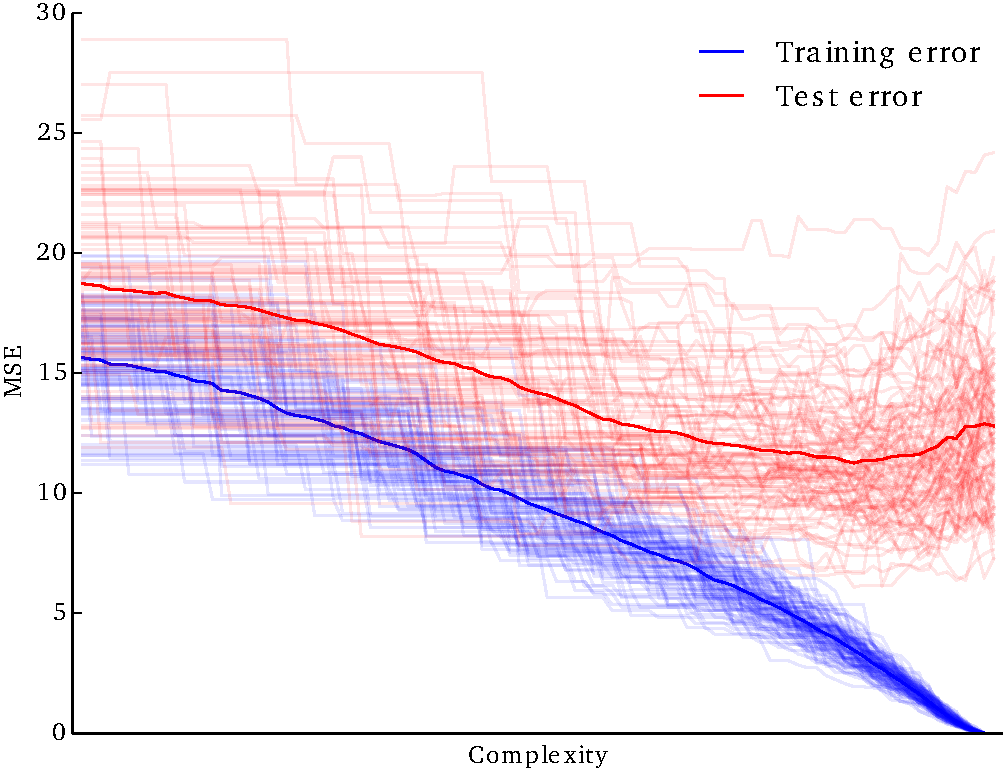
\includegraphics[scale=0.5]{figures/ch2_train_test_error.pdf}
    \caption{Training and test error with respect to the complexity
             of a model. The light blue curves show the training error over
             ${\cal L}_\text{train}$ while the light red curves show the test
             error over ${\cal L}_\text{test}$ for $100$ pairs for training
             and test sets ${\cal L}_\text{train}$ and ${\cal L}_\text{test}$
             drawn at random from a known distribution. The thick blue curve
             is the average training error while the thick red curve is the
             average test error. (Figure inspired from \citep{hastie:2005}.) }
    \label{fig:train-test-error}
\end{figure}

As Figure~\ref{fig:train-test-error}
illustrates, this phenonemon can be observed by examining the
respective training and test estimates of the model with respect to its
complexity. When the model is too simple, both the training and test estimates
are large because of underfitting. As complexity increases, the model gets more
accurate and both the training and test estimates decrease. However, when the
model becomes too complex, specific trends from the training set get captured,
reducing the corresponding training estimates down to $0$, as if the model were
perfect. At the same time, the test estimates become worse because the
structure learned from the training set is actually too speficic and does not
generalize. The model is overfitting. The best parameter value $\theta$ is
therefore the one making the appropriate trade-off and producing a model which
neither too simple nor to complex.

\subsection{Selecting and evaluating simultaneously}
On real applications, and in particular when reporting results, it usually
happens that one wants to do both model selection and model assessment. That
is, having chosen a final model ${\cal A}(\widehat{\theta}^*, {\cal L})$, one
wants to also estimate its generalization error.

A naive assessment of the generalization error of the selected model might be
to simply use the test sample estimate $\smash{\widehat{Err}^\text{test}_{\cal
L}({\cal A}(\widehat{\theta}^*, {\cal L}))}$ (i.e., $\overline{E}({\cal
A}(\widehat{\theta}^*, {\cal L}_\text{train}), {\cal L}_\text{test})$) that was
minimized during model selection. The issue with this estimate is that the
learned model is not independent from ${\cal L}_\text{test}$ since its repeated
construction was precisely guided by the minimization of the prediction error
over ${\cal L}_\text{test}$. As a result, the minimized test sample error is in
fact a biased, optimistic, estimate of the true generalization error, sometimes
leading substantial understimations. For the same reasons, using the $K$-fold
cross-validation estimate does not provide a better estimate since model
selection was similarly guided by the minimization of this quantity.

To guarantee an unbiased estimate, the test set on which the generalization
error is evaluated should ideally be kept out of the entire model selection
procedure and only be used once the final model is selected.
Algorithm~\ref{algo:train-valid-test} details such a protocol. Similarly,
per-fold estimates of the generalization error should be kept out of the model
selection procedure, for example using nested cross-validation within each
fold, as explicited in Algorithm~\ref{algo:cv}.

\begin{algorithm}\label{algo:train-valid-test}
Train-Valid-Test set protocol for both model selection and evaluation.

\begin{enumerate}
\item Divide the learning set ${\cal L}$ into three parts
      ${\cal L}_\text{train}$, ${\cal L}_\text{valid}$ and ${\cal L}_\text{test}$;
\item Perform model selection on ${\cal L}_\text{train} \cup {\cal L}_\text{valid}$
      using test sample estimates, i.e., find:
      \begin{align}
      \widehat{\theta}^* &= \argmin_{\theta} \widehat{Err}_{{\cal L}_\text{train} \cup {\cal L}_\text{valid}}^\text{test}({\cal A}(\theta, {\cal L}_\text{train} \cup {\cal L}_\text{valid})) \\
                         &= \argmin_{\theta} \overline{E}({\cal A}(\theta, {\cal L}_\text{train}), {\cal L}_\text{valid});
      \end{align}
\item Evaluate the (unbiased) generalization error of the final model as
      \begin{equation}
      \overline{E}({\cal A}(\widehat{\theta}^*, {\cal L}_\text{train} \cup {\cal L}_\text{valid}), {\cal L}_\text{test});
      \end{equation}
\item Learn the final model ${\cal A}(\widehat{\theta}^*, {\cal L})$ on the entire learning set.
\end{enumerate}
\end{algorithm}

\begin{algorithm}\label{algo:cv}
Nested $K$-fold cross-validation protocol for both model selection and evaluation.

\begin{enumerate}
\item Divide the learning set ${\cal L}$ into $K$ folds ${\cal L}_1, ..., {\cal L}_K$;
\item For each fold $k=1, ..., K$:
    \begin{enumerate}
        \item Divide ${\cal L}\setminus{\cal L}_k = {\cal L}^{-k}$ into $K$ folds ${\cal L}_1^{-k}, ..., {\cal L}_K^{-k}$;
        \item Perform model selection on the subset ${\cal L}^{-k}$ using nested $K$-fold estimates, i.e., find:
        \begin{align}
            \widehat{\theta}_k^* &= \argmin_{\theta} \widehat{Err}_{{\cal L}_k}^{CV}({\cal A}(\theta, {\cal L}^{-k}))\\
                                 &= \argmin_{\theta} \frac{1}{K} \sum_{l=1}^K \overline{E}({\cal A}(\theta, {\cal L}^{-k} \setminus {\cal L}_l^{-k}), {\cal L}_l^{-k});
        \end{align}
        \item Evaluate the generalization error of the selected sub-model as
        \begin{equation}
            \overline{E}({\cal A}(\widehat{\theta}^*_k, {\cal L}\setminus{\cal L}_k), {\cal L}_k);
        \end{equation}
    \end{enumerate}
\item Evaluate the (unbiased) generalization error of the selected model as the average generalization estimate of the sub-models selected over the folds:
\begin{equation}
\frac{1}{K} \sum_{k=1}^K \overline{E}({\cal A}(\widehat{\theta}^*_k, {\cal L}\setminus{\cal L}_k), {\cal L}_k);
\end{equation}
\item Perform model selection on the entire learning set ${\cal L}$ using $K$-fold cross-validation estimates, i.e., find:
\begin{align}
    \widehat{\theta}^* &= \argmin_{\theta} \widehat{Err}_{\cal L}^{CV}({\cal A}(\theta, {\cal L}))\\
                       &= \argmin_{\theta} \frac{1}{K} \sum_{k=1}^K \overline{E}({\cal A}(\theta, {\cal L} \setminus {\cal L}_k), {\cal L}_k);
\end{align}
\item Learn the final model ${\cal A}(\widehat{\theta}^*, {\cal L})$ on the entire learning set.
\end{enumerate}
\end{algorithm}


\section{Classes of algorithms}

As introduced in Section~\ref{sec:model-selection}, classes of  learning
algorithms can be defined in terms of the space ${\cal H}$ of hypotheses  they
are built upon. Before focusing in the next chapters on one of these classes,
we briefly review in this section the main learning algorithms that have now
matured in the field, including linear models, the $k$-nearest neighbor
algorithm, neural networks and tree-based methods.


\subsection{Linear methods}

\citep{maccullagh:1989,hastie:2005,bishop:2006}

% generalized linear models

\subsection{$k$-nearest neighbors}

% T. Cover and P. Hart. Nearest neighbor pattern classification

\subsection{Neural networks}

% perceptron
% The perceptron: a probabilistic model for information storage and organization in the brain.

% see bishop chapter 5

% deep learning

% Representation Learning: A Review and New Perspectives, Yoshua Bengio, Aaron Courville, Pascal Vincent, Arxiv, 2012.
% The monograph or review paper Learning Deep Architectures for AI (Foundations & Trends in Machine Learning, 2009).
% Deep Machine Learning – A New Frontier in Artificial Intelligence Research – a survey paper by Itamar Arel, Derek C. Rose, and Thomas P. Karnowski.

\subsection{Tree-based methods}

% single
% ensemble
% boosting

\chapter{Classification and regression trees}\label{ch:cart}

\begin{remark}{Outline}
In this chapter, we present a unified framework in which we detail (single)
decision trees methods. In Section~\ref{sec:3:introduction}, we first give an
overview of the context in which these algorithms have been developed. In
Section~\ref{sec:3:tree-structured-models}, we proceed with a mathematical
presentation, introducing all necessary concepts and notations. The general
learning algorithm is then presented in Section~\ref{sec:3:induction} while
more advanced concepts are discussed in finer details in Sections~\ref{sec:3:splitting-rules}
and \ref{sec:3:criteria}. As such, specific algorithms (e.g.,
CART, ID3 or C4.5) are described as specializations of the general framework
presented here.
\end{remark}

\section{Introduction}
\label{sec:3:introduction}

Since always, artificial intelligence has been driven by the ambition to
understand and uncover complex relations in data. That is, to find models that
can not only produce accurate predictions, but also be used to extract
knowledge in an intelligible way. Guided with this twofold objective, research
in machine learning has given rise to extensive bodies works in a myriad of
directions. Among all of them however, tree-based methods stand as one of
the most effective and useful method, capable to produce both reliable and
understandable results, on mostly any kind of data.

Historically, the appearance of \textit{decision trees} is due to
\citet{morgan:1963}, who first proposed a tree-based method called
\textit{automatic interaction dectector} (AID) for handling multi-variate
non-additive effects in the context of survey data. Building upon AID,
methodological improvements and computer programs for exploratory analysis were
then proposed in the following years by several
authors~\citep{sonquist:1970,messenger:1972,gillo:1972,sonquist:1974}. Without
contest however, the principal investigators that have driven research on the modern
methodological principles are \citet{breiman:1978a,breiman:1978b},
\citet{friedman:1977,friedman:1979} and \citet{quinlan:1979,quinlan:1986} who
simultaneously and independently proposed very close algorithms for the
induction of tree-based models. Most notably, the unifying work of
\citet{breiman:1984}, later complemented with the work of \citet{quinlan:1993},
have set decision trees into a simple and consistent methodological framework,
which largely contributed in making them easy to understand and easy to use by
a large audience.

As we will explore in further details all throughout this work, the success
of decision trees (and by extension, of all tree-based methods) is explained
by several factors that make them quite attractive in practice:
\begin{itemize}
\item Decision trees are non-parametric. They can model arbitrarily complex relations between inputs and outputs, without any a priori assumption;
\item Decision trees handle heterogeneous data (ordered or categorical variables, or a mix of both);
\item Decision trees intrinsically implement feature selection, making them robust to irrelevant or noisy variables;
\item Decision trees are robust to outliers or errors in labels;
\item Decision trees are easily interpretable, even for non-statistically oriented users.
\end{itemize}

Most importantly, decision trees are at the foundation of
many modern and state-of-the-art algorithms, including forests of randomized
trees (on which this work is about, see Chapter~\ref{ch:forest}) or
boosting methods~\citep{freund:1995,friedman:2001}, where they are used
as building blocks for composing larger models. Understanding all algorithmic
details of single decision trees is therefore an expected prerequisite
for an in-depth analysis of these methods.


\section{Tree structured models}
\label{sec:3:tree-structured-models}

When the output space is a finite set of values, like in classification where
${\cal Y} = \{c_1, c_2, ..., c_J\}$, another way of looking at a supervised
learning problem is to notice that $Y$ defines a partition over the input space ${\cal X}$, that
is
\begin{equation}
{\cal X} = {\cal X}_{c_1} \cup {\cal X}_{c_2} \cup ... \cup {\cal X}_{c_J},
\end{equation}
where ${\cal X}_{c_k}$ is the set of objects $\mathbf{x}$ for which
$Y$ has value $c_k$. Similarly, a classifier $\varphi$ can also be
regarded as a partition of the input space
${\cal X}$ since it defines an approximation $\widehat{Y}$ of $Y$, which in
turn partitions ${\cal X}$, that is
\begin{equation}\label{eqn:3:partition}
{\cal X} = \widehat{{\cal X}_{c_1}} \cup \widehat{{\cal X}_{c_2}} \cup ... \cup \widehat{{\cal X}_{c_J}},
\end{equation}
where
$\widehat{{\cal X}_{c_k}}$ is the set of objects $\mathbf{x}$ such that
$\varphi(\mathbf{x}) = c_k$. Accordingly, learning a classifier can thus
be restated as learning a partition of ${\cal X}$ matching as closely as
possible the (true) partition engendered by $Y$ over ${\cal X}$.

\begin{remark}{Partitioning with noise}
Notice that when $Y$ cannot be univocally determined given $X=\mathbf{x}$,
e.g., when there is noise on $Y$, then the subsets ${\cal X}_{c_k}$ are not
necessarily disjoints. There may exist two distinct objects from the universe $\Omega$ such
that their representations $\mathbf{x}_1$ and $\mathbf{x}_2$ in the input space
are equal, yet such that the corresponding output values $y_1$ and $y_2$ are different.
By contrast, since $\varphi$ defines a function from ${\cal X}$ to ${\cal Y}$,
any input $\mathbf{x} \in {\cal X}$ is mapped to exactly one output value $y \in
{\cal Y}$ and the subsets $\widehat{{\cal X}_{c_k}}$ are therefore necessarily
disjoints, which means that no model will ever perfectly predict the true output
value in all cases. As discussed in Section~\ref{sec:2:bayes-model}, this
limitation is unavoidable and can in fact be viewed as the cause of the residual error.
\end{remark}

From a geometrical point of view, the principle of tree structured models is
beautifully simple. It consists in recursively partitioning the input space
${\cal X}$ into subspaces and then assign constant prediction values
$\widehat{y}\in{\cal Y}$ to all objects $\mathbf{x}$ within each terminal
subspace. To make things clearer, let us first define the following concepts:

\begin{definition}
A \emph{tree} is a graph $G=(V,E)$ in which any two vertices (or \emph{nodes})
are connected by exactly one path.
\end{definition}

\begin{definition}
A \emph{rooted tree} is a tree in which one of the nodes has been designated as
the \emph{root}. In our case, we additionally assume that a rooted tree is a
\emph{directed} graph, where all edges are directed away from the root.
\end{definition}

\begin{definition}
If there exists an edge from $t_1$ to $t_2$ (i.e., if $(t_1, t_2)\in E$) then
node $t_1$ is said to be the \emph{parent} of node $t_2$ while node $t_2$ is
said to be a \emph{child} of node $t_1$.
\end{definition}

\begin{definition}
In a rooted tree, a node is said to be \emph{internal} if it has one or more
children and \emph{terminal} if it has no children. Terminal nodes are also
known as \emph{leaves}.
\end{definition}

\begin{definition}
A \emph{binary tree} is a rooted tree where all internal nodes exactly
have two children.
\end{definition}

In those terms, a \textit{tree-structured model} (or \textit{decision tree})
can be defined as a model $\varphi: {\cal X} \mapsto {\cal Y}$ represented by a
rooted tree (often binary, but not necessarily), where any node $t$ represents
a subspace ${\cal X}_t \subseteq {\cal X}$ of the intput space, with the root
node $t_0$ corresponding to ${\cal X}$ itself. Internal nodes $t$ are labeled with a
\textit{split} $s_t$ (taken from a set of questions ${\cal Q}$) dividing the
space ${\cal X}_t$ they each represent into disjoint subspaces respectively
corresponding to each of their children. For instance, the set of all binary
splits is the set ${\cal Q}$ of questions $s$ of the form \textit{``Is
$\mathbf{x} \in {\cal X}_A?$''}, where ${\cal X}_A \subset {\cal X}$ is some
subset of the input space. Any split $s$ of this form divides ${\cal X}_t$ into
two subspaces respectively corresponding to ${\cal X}_t \cap {\cal X}_A$ for
the left child of $t$ and to ${\cal X}_t \cap ({\cal X}\setminus{\cal X}_A)$
for the right child of $t$. Terminal nodes are labeled with a best guess value
$\widehat{y}_t \in {\cal Y}$ of the output variable. If $\varphi$ is a
classification tree, then $\widehat{y}_t \in \{ c_1, ..., c_J \}$ while if
$\varphi$ is a regression tree, then $\widehat{y}_t \in \mathbb{R}$. As such,
the predicted output value $\varphi(\mathbf{x})$
is the label of the leaf reached by the instance $\mathbf{x}$ when it is propagated through
the tree by following the splits $s_t$ (see Algorithm~\ref{algo:prediction}).

\begin{algorithm}\label{algo:prediction}
Prediction of the output value $\widehat{y} =\varphi(\mathbf{x})$ in a decision tree.
\textnormal{
\begin{algorithmic}[1]
\Function{Predict}{$\varphi, \mathbf{x}$}
    \State $t \gets t_0$;
    \While{$t$ is not a terminal node}
        \State $t \gets$ the child node $t'$ of $t$ such that $\mathbf{x} \in {\cal X}_{t'}$;
    \EndWhile
    \State \Return $\widehat{y}_t$;
\EndFunction
\end{algorithmic}
}
\end{algorithm}

\begin{remark}{Induction graphs}
From a graph theory point of view, decision trees belong to a larger family
of methods known as \textit{induction graphs}~\citep{zighed:2000}. In this more
general framework, the structure is a directed acyclic graph, which allows for
nodes to be both divided and recombined.
\end{remark}

\begin{figure}
    \centering
    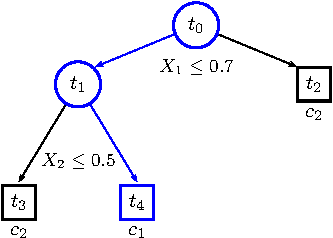
\includegraphics[scale=1.0]{figures/ch3_tree.pdf}
    \caption{A decision tree $\varphi$ built for a binary classification
             problem from an input space ${\cal X}=[0,1]\times[0,1]$.
             (Figure inspired from \citet{breiman:1984}.)}
    \label{fig:3:tree}
\end{figure}

As an example, Figure~\ref{fig:3:tree} illustrates a decision tree $\varphi$
made of five nodes and partitioning the input space ${\cal X} = {\cal X}_1
\times {\cal X}_2 = [0;1] \times [0; 1]$ for a binary classification problem
(where ${\cal Y}=\{ c_1, c_2 \}$). Node $t_0$ is the root node and corresponds
to the whole input space ${\cal X}_{t_0} = {\cal X}$. It is labeled with the binary
split $X_1 \leq 0.7$ (i.e., the question \textit{``Is $X_1 \leq 0.7$?''}) which divides ${\cal X}_{t_0}$ into two disjoint subsets
${\cal X}_{t_1} \cup {\cal X}_{t_2}$. The first set corresponds to its left
child $t_1$ and represents the set of all input vectors $\mathbf{x} \in {\cal
X}_0$ such that $x_1 \leq 0.7$. Similarly, the second set corresponds to its
right child $t_2$ and represents the set of all input vectors $\mathbf{x} \in
{\cal X}_{t_0}$ such that $x_1 > 0.7$. Likewise, $t_1$ is labeled with the
split $X_2 \leq 0.5$ which further divides ${\cal X}_{t_1}$ into two disjoint
subsets ${\cal X}_{t_3} \cup {\cal X}_{t_4}$ respectively corresponding the
sets of all input vectors $\mathbf{x} \in {\cal X}_{t_1}$ such that $x_2 \leq
0.5$ (resp. $x_2 > 0.5$). Terminal nodes $t_2$, $t_3$ and $t_4$ are represented
by squares labeled with an output value $\widehat{y}_t$. They form together a
partition (as defined by Equation~\ref{eqn:3:partition}) of ${\cal X}$, where
each set $\widehat{{\cal X}_{c_k}}$ is obtained from the union of the subspaces
${\cal X}_t$ of all terminal nodes $t$ such that $\widehat{y}_t = c_k$. In this
case, $\widehat{{\cal X}_{c_1}} = {\cal X}_{t_4}$ while $\widehat{{\cal
X}_{c_2}} = {\cal X}_{t_2} \cup {\cal X}_{t_3}$. As shown in
Figure~\ref{fig:3:partition}, the partition engendered by  $\varphi$ on ${\cal
X}$ divides the input space into subspaces that are more and more class
homogeneous, starting from ${\cal X}$ at the root node,  then ${\cal X}_{t_1}
\cup {\cal X}_{t_2}$ at the second level of tree and finally $({\cal X}_{t_3}
\cup {\cal X}_{t_4})\cup {\cal X}_{t_2}$ at the leaves.  As we will explore in
Section~\ref{sec:3:splitting-rules}, the partition is in this case made of
rectangles because of the nature of the splits $s_t \in {\cal Q}$ dividing the nodes.
Predictions are made by propagating instances through the tree and using as
output value the value labeling the terminal nodes in which they fall
into. For example, an object $\mathbf{x}=(x_1=0.2, x_2=0.7)$ falls into $t_4$
and therefore $\varphi(\mathbf{x}) = \widehat{y}_{t_4} = c_1$.

\begin{figure}
    \centering
    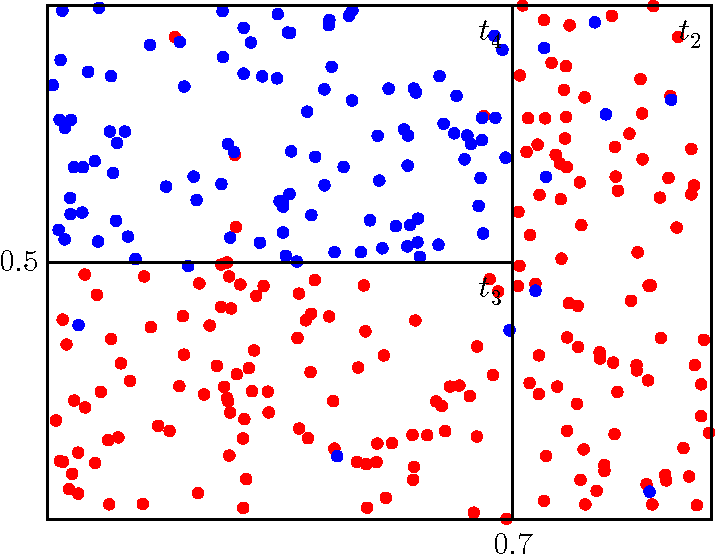
\includegraphics[scale=0.5]{figures/ch3_partition.pdf}
    \caption{Partition of ${\cal X}$ induced by the decision tree $\varphi$.
             Blue dots correspond to objects of class $c_1$ while red dots correspond
             to objects of class $c_2$. (Figure inspired from \citet{breiman:1984}.)}
    \label{fig:3:partition}
\end{figure}


\section{Induction of decision trees}
\label{sec:3:induction}

Learning a decision tree ideally amounts to determine the tree structure which
produces the partition which is closest to the partition engendered by $Y$ over
${\cal X}$. Since it is unknown however, the construction of a decision tree is usually
driven instead with the objective of finding a model which partitions the
learning set ${\cal L}$ as best as possible. Among all decision trees $\varphi
\in {\cal H}$ however, there may exist several of them that explain ${\cal L}$
equally best. Following Occam's Razzor principles~\citep{blumer:1987} of prefering the explanation
which makes as few assumptions as possible, that is to favor the simplest
solution that fits the data, learning a decision tree from ${\cal L}$ is then
usually restated as finding the smallest tree $\varphi^*$ (in terms of internal nodes) minimizing its
resubstitution estimate $\overline{E}(\varphi^*, {\cal L})$. While this
assumption makes sense from a generalization point of view, it also makes
sense regarding interpretability. A decision tree which is small is easier
to understand than a large and complex tree.

As shown by \citet{hyafil:1976} however, finding the smallest tree $\varphi^*$
that minimizes its resubstitution estimate is an NP-complete problem. As a
consequence, under the assumption that $P \neq NP$, there exists no efficient
algorithm for finding $\varphi^*$, thereby suggesting that finding efficient heuristics
for constructing near-optimal decision trees is the best solution to keep computation
requirements within realistic boundaries.

Following the framework of \citet{breiman:1984}, let us broadly define an \textit{impurity} measure $i(t)$ as a
non-negative function that evaluates the goodness of any node $t$. Let assume that
the smaller $i(t)$, the \textit{purer} the node and the better the predictions
$\widehat{y}_t(\mathbf{x})$ for all $\mathbf{x} \in {\cal L}_t$, where ${\cal
L}_t$ is the subset of learning samples falling into $t$, that is all
$(\mathbf{x}, y) \in {\cal L}$ such that $\mathbf{x} \in {\cal X}_t$.

Starting from a single node representing the whole learning set  ${\cal L}$,
near-optimal decision trees can then be grown greedily by iteratively dividing
nodes into purer nodes. That is, to iteratively  divide into smaller subsets the
subsets of ${\cal L}$ represented by the nodes, until all terminal nodes cannot
be made purer, hence guaranting near-optimal predictions over ${\cal L}$. The
greedy assumption to make the resulting tree as small as possible, thereby
seeking for good generalization, is then to divide each node $t$ using the
split $s^*$ that locally maximizes the decrease of impurity of the resulting child nodes.

Formally, the decrease of impurity of a binary split $s$ is defined as follows:

\begin{definition}\label{def:impurity-decrease}
The \emph{impurity decrease} of a binary split $s \in {\cal Q}$ dividing node $t$ into
a left node $t_L$ and a right node $t_R$ is
\begin{equation}
\Delta i(s, t) = i(t) - p_L i(t_L) - p_R i(t_R)
\end{equation}
where $p_L$ (resp., $p_R$) is the proportion $\tfrac{N_{t_L}}{N_t}$ (resp., $\tfrac{N_{t_R}}{N_t}$)
of learning samples from ${\cal L}_t$ going to $t_L$ (resp., to $t_R$) and where $N_t$
is the size of the subset ${\cal L}_t$.
\end{definition}

On the basis of this concept, a general greedy procedure for the induction of
decision trees can now be described formally as outlined in
Algorithm~\ref{algo:induction}. Note that for the sake of clarity,
Algorithm~\ref{algo:induction} is formulated in terms of binary splits.
However, as we will explore later in Section~\ref{sec:3:splitting-rules}, it
generalizes naturally to $n$-ary splits.

\begin{algorithm}\label{algo:induction}
Greedy induction of a binary decision tree.
\textnormal{
\begin{algorithmic}[1]
\Function{BuildDecisionTree}{${\cal L}$}
    \State Create a decision tree $\varphi$ with root node $t_0$;
    \State Create an empty stack $S$ of \emph{open} nodes $(t, {\cal L}_t)$ ;
    \State $S$\Call{.push}{($t_0, {\cal L}$)}
    \While{$S$ is not empty}
        \State $t, {\cal L}_t \gets$ $S$\Call{.pop}{~}
        \If{the stopping criterion is met for $t$}\label{algo:induction:stop}
            \State $\widehat{y}_{t} \gets$ some constant value;\label{algo:induction:terminal}
        \Else
            \State Find the split that maximizes impurity decrease $$s^* = \argmax_{s \in {\cal Q}} \Delta i(s, t);$$ \label{algo:induction:split}
            \State Partition ${\cal L}_t$ into ${\cal L}_{t_L} \cup {\cal L}_{t_R}$ according to $s^*$;
            \State Create the left child node $t_L$ of $t$;
            \State Create the right child node $t_R$ of $t$;
            \State $S$\Call{.push}{($t_R, {\cal L}_{t_R}$)};
            \State $S$\Call{.push}{($t_L, {\cal L}_{t_L}$)};
        \EndIf
    \EndWhile
    \State \Return $\varphi$;
\EndFunction
\end{algorithmic}
}
\end{algorithm}

The rest of this chapter is now dedicated to a detailed discussion of specific
parts of Algorithm~\ref{algo:induction}. Section~\ref{sec:3:assignment}
discusses assignment rules for terminal nodes
(Line~\ref{algo:induction:terminal} of Algorithm~\ref{algo:induction}) while
Section~\ref{sec:3:stop} outlines stopping criteria for deciding when a node
becomes terminal (Line~\ref{algo:induction:stop} of
Algorithm~\ref{algo:induction}). Section~\ref{sec:3:splitting-rules} then
presents families ${\cal Q}$ of splitting rules along with exact and
approximate strategies for finding the best split $s^* \in {\cal Q}$
(Line~\ref{algo:induction:split} of Algorithm~\ref{algo:induction}). Finally,
Section~\ref{sec:3:criteria} describes  impurity criterion $i(t)$ to evaluate
the goodness of splits. As we will see, assigning values to terminal
nodes happens to be quite simple. The crux of the problem is in finding good
splits and in knowing when to stop splitting.


\section{Assignment rules}
\label{sec:3:assignment}

Let us assume that node $t$ has been declared terminal given some stopping
criterion (See Section~\ref{sec:3:stop}). The next step
(Line~\ref{algo:induction:terminal} of Algorithm~\ref{algo:induction}) in the
induction procedure is to label $t$ with a constant value $\widehat{y}_t$ to
be used as a prediction of the output variable $Y$. As such, node $t$ can  be
regarded as a simplistic model defined locally on ${\cal X}_t \times {\cal Y}$
and producing the same output value $\widehat{y}_t$ for all possible input
vectors falling into $t$.

Let us first notice that, for a tree $\varphi$ of \textit{fixed} structure,
minimizing the global generalization error is strictly equivalent to minimizing
the local generalization error of each simplistic model in the terminal nodes.
Indeed,
\begin{align}
Err_{\cal L}(\varphi) &= \mathbb{E}_{X,Y} \{ L(Y, \varphi(X)) | {\cal L} \} \nonumber \\
                      &= \sum_{t \in \widetilde{\varphi}} P(X \in {\cal X}_t) \mathbb{E}_{X,Y|t} \{ L(Y, \widehat{y}_t) | {\cal L} \} \label{eqn:assignment-generalization}
\end{align}
where $\widetilde{\varphi}$ denotes the set of terminal nodes in $\varphi$
and where the inner expectation\footnote{The joint expectation of $X$ and $Y$
is taken over all objects $i \in \Omega$ such $\mathbf{x}_i \in {\cal X}_t$.}
is the local generalization error of the model at node $t$. In this later form,
a model which minimizes $Err_{\cal L}(\varphi)$ is a model which minimizes the inner
expectation leaf-wise. Learning the best possible decion tree (of
fixed structure) therefore simply amounts to find the best constants
$\widehat{y}_t$ at each terminal node.

\subsection{Classification}

When $L$ is the zero-one loss, the inner expectation in Equation~\ref{eqn:assignment-generalization}
is minimized by the plurality rule:
\begin{align}
\widehat{y}_t^* &= \argmin_{c \in {\cal Y}} \mathbb{E}_{X, Y|t}\{ 1(Y, c) | {\cal L} \} \nonumber \\
                &= \argmin_{c \in {\cal Y}} P(Y \neq c | X \in {\cal X}_t) \nonumber \\
                &= \argmax_{c \in {\cal Y}} P(Y = c | X \in {\cal X}_t)\label{eqn:assignment-classification}
\end{align}
Put otherwise, the generalization error of $t$ is minimized by predicting
the class which is the most likely for the samples in the subspace of $t$.
Note that if the maximum is achieved by two or more different classes, then
$\widehat{y}_t^*$ is assigned arbitrarily as any one of the maximizing classes.

Once again, Equation~\ref{eqn:assignment-classification} cannot be solved
without the probability distribution $P(X, Y)$. However, its solution can be
approximated by using estimates of $P(Y=c|X \in {\cal X}_t)$. Let $N_t$ denotes
the number of objects in ${\cal L}_t$ and let $N_{ct}$ denotes the number of
objects of class $c$ in ${\cal L}_t$. Then, the proportion
$\tfrac{N_{ct}}{N_t}$ can be interpreted as the estimated probability\footnote{Lower case $p$ denotes an estimated probability while upper case $P$ denotes a theoretical probability.}
$p(Y=c|X\in{\cal X}_t)$ (shortly denoted $p(c|t)$) of class $c$ in $t$ and therefore be used to solve
Equation~\ref{eqn:assignment-classification}:
\begin{align}\label{eqn:assignement-classification-approx}
\widehat{y}_t &= \argmax_{c \in {\cal Y}} p(c | t)
\end{align}

Similarly, let us also define the proportion $\tfrac{N_t}{N}$ as the estimated
probability $p(X \in {\cal X}_t)$ (shortly denoted $p(t)$). Plugging this
estimate into Equation~\ref{eqn:assignment-generalization} and approximating
the local generalization error with $1 - p(\widehat{y}_t | t)$ as done
above, it follows:
\begin{align}
\widehat{Err}_{\cal L}(\varphi) &= \sum_{t \in \widetilde{\varphi}} p(t) (1 - p(\widehat{y}_t | t)) \nonumber \\
    &= \sum_{t \in \widetilde{\varphi}} \frac{N_t}{N} (1 - \frac{N_{{\widehat{y}_t}t}}{N_t}) \nonumber \\
    &= \frac{1}{N} \sum_{t \in \widetilde{\varphi}} N_t - N_{{\widehat{y}_t}t} \nonumber \\
    &= \frac{1}{N} \sum_{t \in \widetilde{\varphi}} \sum_{\mathbf{x}_i, y_i \in {\cal L}_t} 1(y_i \neq \widehat{y}_t) \nonumber \\
    &= \frac{1}{N} \sum_{\mathbf{x}_i, y_i \in {\cal L}} 1(y_i \neq \varphi(t)) = \widehat{Err}_{\cal L}^\text{train}(\varphi) \label{eqn:train-error-tree}
\end{align}
In other words, approximating Equation~\ref{eqn:assignment-generalization}
through probability estimates computed from class proportions in ${\cal L}$ is
equivalent to the resubstitution estimate of $\varphi$
(Equation~\ref{eqn:training-error}). As a consequence, assignement
rule~\ref{eqn:assignement-classification-approx} in fact minimizes this latter quantity rather than the
true generalization error.

An important property of assignment rule~\ref{eqn:assignement-classification-approx} is
that the more one splits a terminal node \textit{in any way}, the smaller
$\smash{\widehat{Err}_{\cal L}^\text{train}(\varphi)}$ becomes.

\begin{proposition}
For any split of $t$ into $t_L$ and $t_R$
\begin{equation}
p(t)(1 - p(\widehat{y}_t | t)) \geq p(t_L)(1 - p(\widehat{y}_{t_L} | t_L)) + p(t_L)(1 - p(\widehat{y}_{t_R} | t_R))
\end{equation}
with equality if $\widehat{y}_t = \widehat{y}_{t_L} = \widehat{y}_{t_R}$ \citep{breiman:1984}.
\end{proposition}

\begin{proof}
Hi
\end{proof}

\subsection{Regression}

% Breiman 230+


\section{Stopping criteria}
\label{sec:3:stop}

%       Simplest approaches:
%           - L_t cannot be split more (eg., X is constant)
%           - min_samples_split (aka nmin)
%           - max_depth
%           - max_nodes?
%       CART 37+, chapter 3
%       * Critères d'arrêts [ différents paramètres, chi² ]
%       Zighed: page 100+
%       Pre-pruning vs. Post-pruning (brief discussion)


\section{Splitting rules}
\label{sec:3:splitting-rules}

%     > Splitting nodes
%         [ max_features, min_samples_leaf ]
%         - set of questions / answers
%               + categorical vs continuous)
%               + bi-partitions vs n-partitions
%               + weak learners
%         - Best splits
%             + Greedy approximation of optimal trees
%             + optimizing locally the impurity <=> optimizing globally? see page 33+
%         - Approximately best splits
%             + Binning
%             + Subsampling

\section{Goodness of split}
\label{sec:3:criteria}

%     > Impurity criteria
%           Voir chapitres 9+ Zighed
%         - pourquoi pas simplifier utiliser l'erreur de resubstitution?
%         - Gini, Entropy, Variance, Information gain etc (see cart + graphes)
%         - Effet du critère sur les cuts
%             End-cut preference (CART 11.8)
%             Normalisation par l'entropy (cf. Vincent, Louis)
%             Effet sur la structure des arbres générés
%         - Sample weighting
%             Negative weights? (@ndawe)

% \section{Interpreting decision trees}
% % From trees to rules

\chapter{Random Forests}\label{ch:forest}

\begin{remark}{Outline}
In this chapter, we present the well-known family of \textit{random forests}
methods. In Section~\ref{sec:4:bias-variance}, we first describe the bias-variance
decomposition of the prediction error and then present, in
Section~\ref{sec:4:ensemble}, how aggregating randomized models through
ensembles reduces the prediction error by decreasing the variance term in this
decomposition. In Section~\ref{sec:4:random-forests}, we revisit random forests
and its variants and study how randomness introduced into the decision trees
reduces prediction errors by decorrelating the decision
trees in the ensemble. Properties and features of random forests are then outlined
in Section~\ref{sec:4:features} while their consistency
is finally explored in Section~\ref{sec:4:consistency}.
\end{remark}


\section{Bias-variance decomposition}
\label{sec:4:bias-variance}

In section~\ref{sec:2:performance-evaluation}, we defined the generalization
error of a model $\varphi_{\cal L}$ as its expected prediction error
according to some loss function $L$
\begin{equation}\label{eqn:4:generalization-error}
Err(\varphi_{\cal L}) = \mathbb{E}_{X,Y} \{ L(Y, \varphi_{\cal L}(X)) \}.
\end{equation}
Similarly, the expected prediction error of $\varphi_{\cal L}$ at $X=\mathbf{x}$
can be expressed as
\begin{equation}
Err(\varphi_{\cal L}(\mathbf{x})) = \mathbb{E}_{Y|X=\mathbf{x}} \{ L(Y, \varphi_{\cal L}(\mathbf{x})) \}.\label{eqn:4:generalization-error:x}
\end{equation}

In regression, for the squared error loss, this latter form of the expected
prediction error additively decomposes into bias and variance terms which
together constitute a very useful framework for diagnosing the prediction error
of a model. In classification, for the zero-one loss, a similar decomposition
is more difficult to obtain. Yet, the concepts of bias and variance can be
transposed in several ways to classification, thereby providing comparable
frameworks for studying the prediction error of classifiers.


\subsection{Regression}
\label{sec:bias-variance:regression}

In regression, assuming that $L$ is the squared error loss, the expected
prediction error of a model $\varphi_{\cal L}$ at a given point $X=\mathbf{x}$
can be rewritten with respect to the Bayes model $\varphi_B$:
\begin{align}
& Err(\varphi_{\cal L}(\mathbf{x})) \nonumber \\
&= \mathbb{E}_{Y|X=\mathbf{x}} \{ (Y - \varphi_{\cal L}(\mathbf{x}))^2 \} \nonumber \\
&= \mathbb{E}_{Y|X=\mathbf{x}} \{ (Y -\varphi_B(\mathbf{x}) + \varphi_B(\mathbf{x}) - \varphi_{\cal L}(\mathbf{x}))^2 \} \nonumber \\
&= \mathbb{E}_{Y|X=\mathbf{x}} \{ (Y -\varphi_B(\mathbf{x}))^2  \} + \mathbb{E}_{Y|X=\mathbf{x}} \{ (\varphi_B(\mathbf{x}) - \varphi_{\cal L}(\mathbf{x}))^2 \} \nonumber \\
& \hookrightarrow + \mathbb{E}_{Y|X=\mathbf{x}} \{ 2 (Y - \varphi_B(\mathbf{x}))(\varphi_B(\mathbf{x}) - \varphi_{\cal L}(\mathbf{x})) \} \nonumber \\
&= \mathbb{E}_{Y|X=\mathbf{x}} \{ (Y -\varphi_B(\mathbf{x}))^2 \} + \mathbb{E}_{Y|X=\mathbf{x}} \{ (\varphi_B(\mathbf{x}) - \varphi_{\cal L}(\mathbf{x}))^2 \} \nonumber \\
&= Err(\varphi_B(\mathbf{x})) +  (\varphi_B(\mathbf{x}) - \varphi_{\cal L}(\mathbf{x}))^2 \label{eqn:4:decomp1}
\end{align}
since $\mathbb{E}_{Y|X=\mathbf{x}} \{ Y - \varphi_B(\mathbf{x}) \} =
\mathbb{E}_{Y|X=\mathbf{x}} \{ Y \} - \varphi_B(\mathbf{x}) = 0$ by definition
of the Bayes model in regression. In this form, the first term in the last
expression of Equation~\ref{eqn:4:decomp1} corresponds to the (irreducible)
residual error  at $X=\mathbf{x}$ while the second term represents the
discrepancy of $\varphi_{\cal L}$ from the Bayes model. The farther from the
Bayes model, the more sub-optimal the model and the larger the error.

If we further assume that the learning set ${\cal L}$ is itself a random
variable (sampled from the population $\Omega$) and that the learning algorithm is deterministic, then the expected
discrepancy over ${\cal L}$ with the Bayes model can further be re-expressed in terms of the
average prediction $\mathbb{E}_{\cal L} \{ \varphi_{\cal L}(\mathbf{x}) \}$
over the models learned from all possible learning sets of size $N$:
\begin{align}
& \mathbb{E}_{\cal L} \{ (\varphi_B(\mathbf{x}) - \varphi_{\cal L}(\mathbf{x}))^2 \}\nonumber \\
&= \mathbb{E}_{\cal L} \{ (\varphi_B(\mathbf{x}) - \mathbb{E}_{\cal L} \{ \varphi_{\cal L}(\mathbf{x}) \} + \mathbb{E}_{\cal L} \{ \varphi_{\cal L}(\mathbf{x}) \} - \varphi_{\cal L}(\mathbf{x}))^2 \} \nonumber \\
&= \mathbb{E}_{\cal L} \{ (\varphi_B(\mathbf{x}) - \mathbb{E}_{\cal L} \{ \varphi_{\cal L}(\mathbf{x}) \} )^2 \} + \mathbb{E}_{\cal L} \{ (\mathbb{E}_{\cal L} \{ \varphi_{\cal L}(\mathbf{x}) \} - \varphi_{\cal L}(\mathbf{x}))^2 \} \}\nonumber \\
& \hookrightarrow+ \mathbb{E}_{\cal L} \{ 2(\varphi_B(\mathbf{x}) - \mathbb{E}_{\cal L} \{ \varphi_{\cal L}(\mathbf{x}) \})(\mathbb{E}_{\cal L} \{ \varphi_{\cal L}(\mathbf{x}) \} - \varphi_{\cal L}(\mathbf{x}))\} \nonumber \\
&= \mathbb{E}_{\cal L} \{ (\varphi_B(\mathbf{x}) - \mathbb{E}_{\cal L} \{ \varphi_{\cal L}(\mathbf{x}) \} )^2 \} + \mathbb{E}_{\cal L} \{ (\mathbb{E}_{\cal L} \{ \varphi_{\cal L}(\mathbf{x}) \} - \varphi_{\cal L}(\mathbf{x}))^2 \} \}\nonumber \\
&= (\varphi_B(\mathbf{x}) - \mathbb{E}_{\cal L} \{ \varphi_{\cal L}(\mathbf{x}) \} )^2 + \mathbb{E}_{\cal L} \{ (\mathbb{E}_{\cal L} \{ \varphi_{\cal L}(\mathbf{x}) \} - \varphi_{\cal L}(\mathbf{x}))^2 \}
\end{align}
since $\mathbb{E}_{\cal L}\{ \mathbb{E}_{\cal L} \{ \varphi_{\cal
L}(\mathbf{x}) \} - \varphi_{\cal L}(\mathbf{x}) \} =  \mathbb{E}_{\cal L} \{
\varphi_{\cal L}(\mathbf{x}) \} -  \mathbb{E}_{\cal L} \{ \varphi_{\cal
L}(\mathbf{x}) \} = 0$. In summary, the expected generalization error additively
decomposes as formulated in Theorem~\ref{thm:bias-variance}.

\begin{theorem}\label{thm:bias-variance}
For the squared error loss, the bias-variance decomposition of the expected
generalization error $\mathbb{E}_{\cal L} \{ Err(\varphi_{\cal L}(\mathbf{x}))
\}$ at $X=\mathbf{x}$ is
\begin{equation}
\mathbb{E}_{\cal L} \{ Err(\varphi_{\cal L}(\mathbf{x})) \} = \text{noise}(\mathbf{x}) + \text{bias}^2(\mathbf{x}) + \text{var}(\mathbf{x}),
\end{equation}
where
\begin{align*}
\text{noise}(\mathbf{x}) &= Err(\varphi_B(\mathbf{x})), \\
\text{bias}^2(\mathbf{x}) &= (\varphi_B(\mathbf{x}) - \mathbb{E}_{\cal L} \{ \varphi_{\cal L}(\mathbf{x}) \} )^2, \\
\text{var}(\mathbf{x}) &= \mathbb{E}_{\cal L} \{ (\mathbb{E}_{\cal L} \{ \varphi_{\cal L}(\mathbf{x}) \} - \varphi_{\cal L}(\mathbf{x}))^2 \}.
\end{align*}
\end{theorem}

This bias-variance decomposition of the generalization error is due to
\citet{geman:1992} and was first proposed in the context of neural networks.
The first term, $\text{noise}(\mathbf{x})$, is the residual error. It is
entirely independent of both the learning algorithm and the learning set and
provides for any model a theoretical lower bound on its generalization error.
The second term, $\text{bias}^2(\mathbf{x})$, measures the discrepancy between
the average prediction and the prediction of the Bayes model. Finally, the
third term, $\text{var}(\mathbf{x})$, measures the variability of the
predictions at $X=\mathbf{x}$ over the models learned from all possible
learning sets. All three terms are illustrated in Figure~\ref{fig:bias-variance}
for a toy and artificial regression problem. Both $\text{noise}(\mathbf{x})$ and
$\text{var}(\mathbf{x})$ measures the spread of the two densities while
$\text{bias}^2(\mathbf{x})$ is the distance between their means.

\begin{figure}
    \centering
    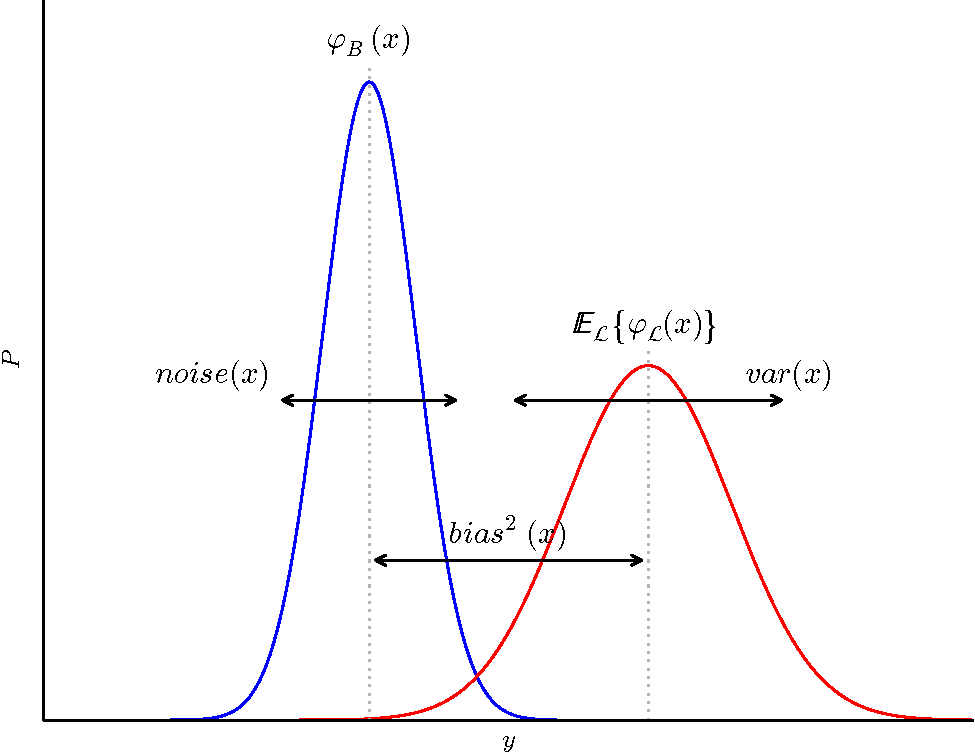
\includegraphics[width=0.9\textwidth]{figures/ch4_bias_variance.pdf}
    \caption{Residual error, bias and variance at $X=\mathbf{x}$. (Figure inspired from \citep{geurts:2002}.)}
    \label{fig:bias-variance}
\end{figure}

As a typical example, the bias-variance decomposition framework can be used as
a tool for diagnosing underfitting and overfitting (as previously introduced in
Section \ref{sec:2:model-selection}). The upper plots in
Figure~\ref{fig:overfitting} illustrate in light red predictions $\varphi_{\cal
L}(\mathbf{x})$ for polynomials of degree $1$, $5$ and $15$ learned over random
learning sets ${\cal L}$ sampled from a noisy cosinus function. Predictions
$\mathbb{E}_{\cal L} \{ \varphi_{\cal L}(\mathbf{x}) \}$ of the average model
are represented by the thick red lines. Predictions for the model learned over
the learning set, represented by the blue dots, are represented in gray.
Predictions of the Bayes model are shown by blue lines and coincide with the unnoised
cosinus function that defines the regression problem. The lower plots in the
figure illustrate the bias-variance decomposition of the expected
generalization error of the polynomials.

\begin{figure}
    \hspace{-0.75cm}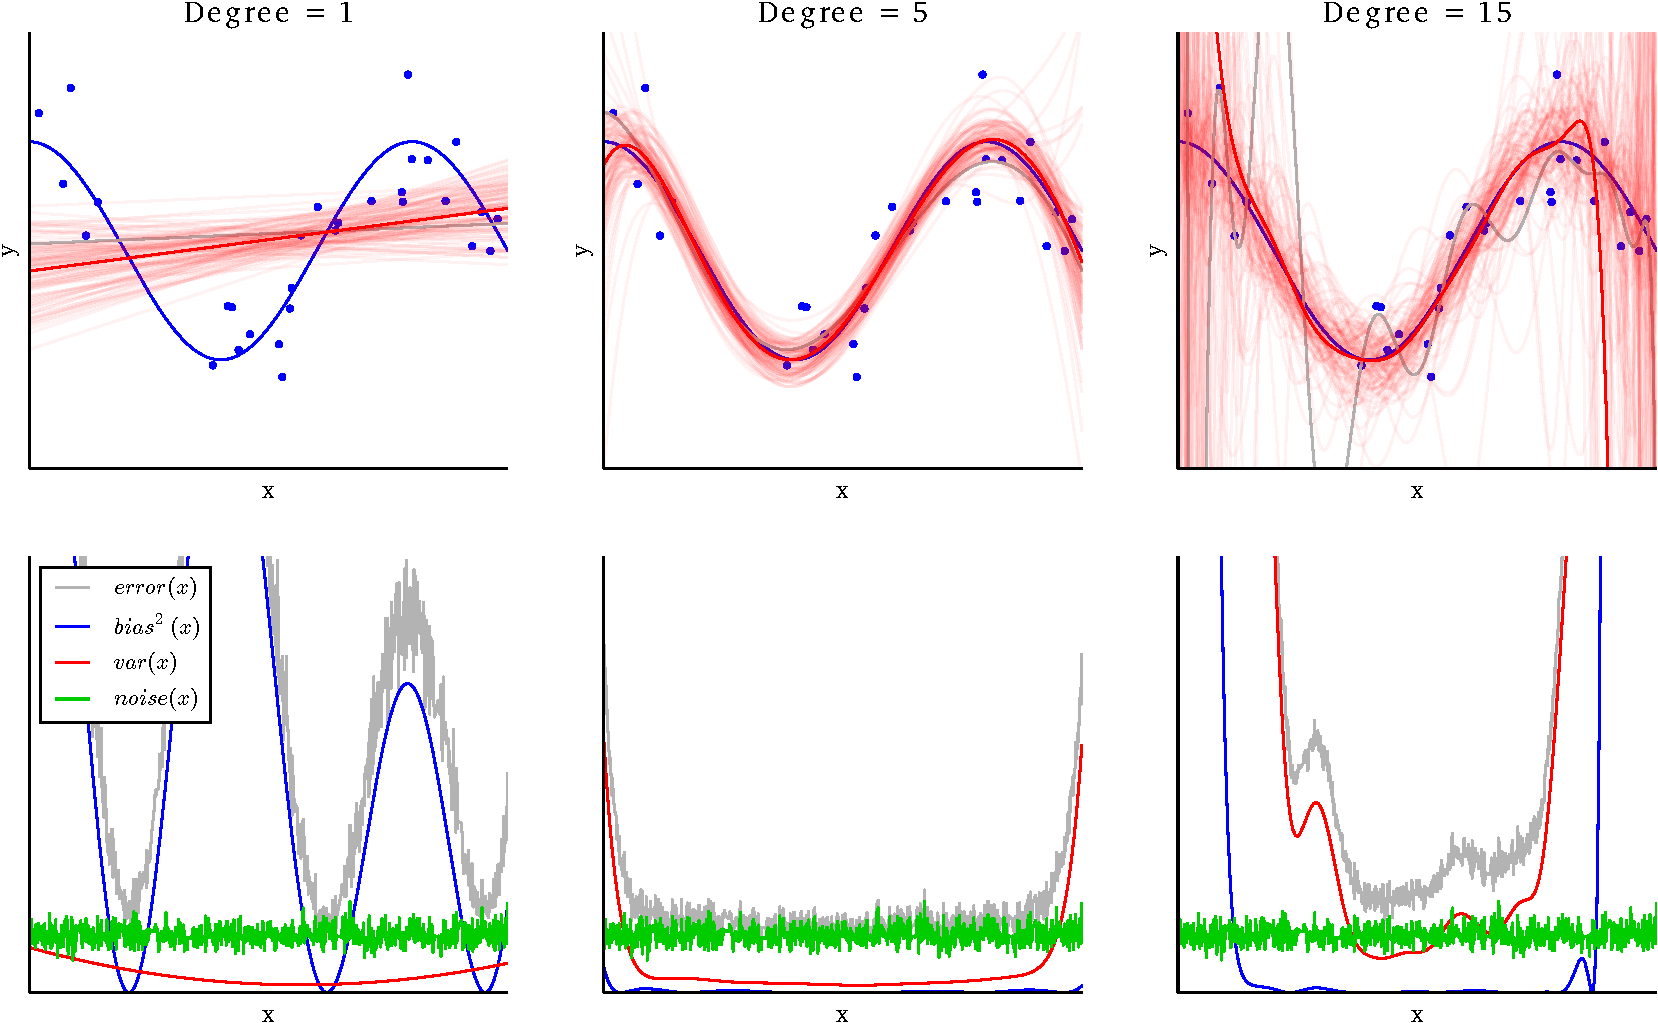
\includegraphics[width=1.1\textwidth]{figures/ch4_overfitting.pdf}
    \caption{Bias-variance decomposition of the expected generalization error for polynomials of degree $1$, $5$ and $15$.}
    \label{fig:overfitting}
\end{figure}

Clearly, polynomials of degree $1$ (left) suffer from underfitting. In terms of
bias and variance, this translates into low variance but high bias as shown in
the lower left plot of Figure~\ref{fig:overfitting}. Indeed, due to the low
degree of the polynomials (i.e., due to the low model complexity), the
resulting models are almost all identical and  the variability of the
predictions from one model to another is therefore quite low. Also, because of
low complexity, none of them really fits the trend of the training points, even
approximately, which implies that the average model is far from approximating
the Bayes model. This results in high bias. On the other hand, polynomials of
degree $15$ (right) suffer from overfitting. In terms of bias and variance, the
situation is the opposite. Predictions have low bias but high variance, as
shown in the lower right plot of Figure~\ref{fig:overfitting}. The variability
of the predictions is large because the high degree of the polynomials (i.e.,
the high model complexity) captures noise in the learning set. Indeed, compare
the gray line with the blue dots -- they almost all intersect. Put otherwise,
small changes in the learning set result in large changes in the obtained model
and therefore in its predictions. By contrast, the average model is now quite
close from the Bayes model, which results in low bias\footnote{Note however the
Gibbs-like phenomenon resulting in both high variance and high bias at the
boundaries of ${\cal X}$.}. Finally, polynomials of degree $5$ (middle) are
neither too simple nor too complex. In terms of bias and variance, the trade-off
is well-balanced between the two extreme situations. Bias and variance are
neither too low nor too large.


\subsection{Classification}
\label{sec:bias-variance:classification}

In direct analogy with the bias-variance decomposition for the squared error
loss, similar decompositions have been proposed in the literature for the
expected generalization error based on the zero-one loss, i.e., for
$\mathbb{E}_{\cal L}\{ \mathbb{E}_{Y|X=\mathbf{x}} \{ 1(\varphi_{\cal L}(x)
\neq Y) \} \} = P_{{\cal L},Y|X=\mathbf{x}}(\varphi_{\cal L}(\mathbf{x}) \neq
Y)$. Most notably, \citet{dietterich:1995}, \citet{breiman:1996},
\citet{kohavi:1996} and \citet{tibshirani:1996} have all developed additive
decompositions similar to Theorem~\ref{thm:bias-variance} by redefining the
concepts of bias and variance in the case of classification. While these
efforts have all provided useful insight into the nature of classification
error, none of them really have provided a seductively as simple and
satisfactory framework as in regression (for reviews, see
\citep{friedman:1997,geurts:2002,james:2003}).

An interesting connection with Theorem~\ref{thm:bias-variance} however is to
remark that classification algorithms usually work by computing estimates
\begin{equation}\label{eqn:4:proba-estimates}
\widehat{p}_{\cal L}(Y=c|X=\mathbf{x})
\end{equation}
of the conditional class probability (e.g.,
$\widehat{p}_{\cal L}(Y=c|X=\mathbf{x}) = p(c|t)$ in decision trees, as defined in Section~\ref{sec:3:assignment}) and then deriving a classification rule by
predicting the class that maximizes this estimate, that is:
\begin{equation}\label{eqn:4:classificaton-rule}
\varphi_{\cal L}(\mathbf{x}) = \argmax_{c \in {\cal Y}} \widehat{p}_{\cal L}(Y=c|X=\mathbf{x})
\end{equation}
As such, a direction for studying classification models is to relate the
bias-variance decomposition of these numerical estimates to the expected
misclassification error of classification rule~\ref{eqn:4:classificaton-rule}.

We now reproduce the results of \citet{friedman:1997} who made this connection
explicit for the case of binary classification. Let us first decompose the
expected classification error into an irreducible part associated with the
random nature of the output $Y$ and a reducible part that depends on
$\varphi_{\cal L}(\mathbf{x})$, in analogy with Equation~\ref{eqn:4:decomp1}
for the squared error loss. (Note that, to simplify notations, we assume that
all probabilities based on the random variable $Y$ is with respect to the
distribution of $Y$ at $X=\mathbf{x}$.)
\begin{align}
& \mathbb{E}_{\cal L}\{ \mathbb{E}_{Y|X=\mathbf{x}} \{ 1(\varphi_{\cal L}(\mathbf{x}) \neq Y) \} \}  \\
&= P_{{\cal L}}(\varphi_{\cal L}(\mathbf{x}) \neq Y) \nonumber \\
&= 1 - P_{{\cal L}}(\varphi_{\cal L}(\mathbf{x}) = Y) \nonumber \\
&= \begin{aligned}[t]
    1 &- P_{\cal L}(\varphi_{\cal L}(\mathbf{x}) = \varphi_B(\mathbf{x})) P(\varphi_B(\mathbf{x})=Y) \nonumber \\
      &- P_{\cal L}(\varphi_{\cal L}(\mathbf{x}) \neq \varphi_B(\mathbf{x})) P(\varphi_B(\mathbf{x})\neq Y) \nonumber
   \end{aligned}\nonumber \\
&= \begin{aligned}[t]
    &P(\varphi_B(\mathbf{x})\neq Y) + P_{\cal L}(\varphi_{\cal L}(\mathbf{x})\neq \varphi_B(\mathbf{x})) \nonumber \\
    &- 2 P_{\cal L}(\varphi_{\cal L}(\mathbf{x})\neq \varphi_B(\mathbf{x})) P(\varphi_B(\mathbf{x})\neq Y)  \nonumber \\
   \end{aligned}\nonumber \\
&= P(\varphi_B(\mathbf{x})\neq Y) + P_{\cal L}(\varphi_{\cal L}(\mathbf{x})\neq \varphi_B(\mathbf{x}))(2 P(\varphi_B(\mathbf{x}) = Y) - 1) \nonumber
\end{align}

In this form, the first term is the irreducible error of the Bayes model. The
second term is the increased error due to the misestimation of the optimal
decision boundary. The probability $P_{\cal L}(\varphi_{\cal L}(\mathbf{x})\neq
\varphi_B(\mathbf{x}))$  is the probability for the model of making a decision
which is different from the decision of the Bayes model. This happens
when the estimate $\widehat{p}_{\cal L}(Y=\varphi_B(\mathbf{x}))$ is lower
than $0.5$, that is:
\begin{equation}\label{eqn:4:prob-diff-from-bayes}
P_{\cal L}(\varphi_{\cal L}(\mathbf{x})\neq \varphi_B(\mathbf{x})) = P_{\cal L}(\widehat{p}_{\cal L}(Y=\varphi_B(\mathbf{x})) < 0.5)
\end{equation}
As Figure~\ref{fig:estimate-distribution} illustrates, probability~\ref{eqn:4:prob-diff-from-bayes}
in fact corresponds to the tail area on the left side
of the decision threshold (at 0.5) of the distribution of the estimate.

\begin{figure}
    \centering
    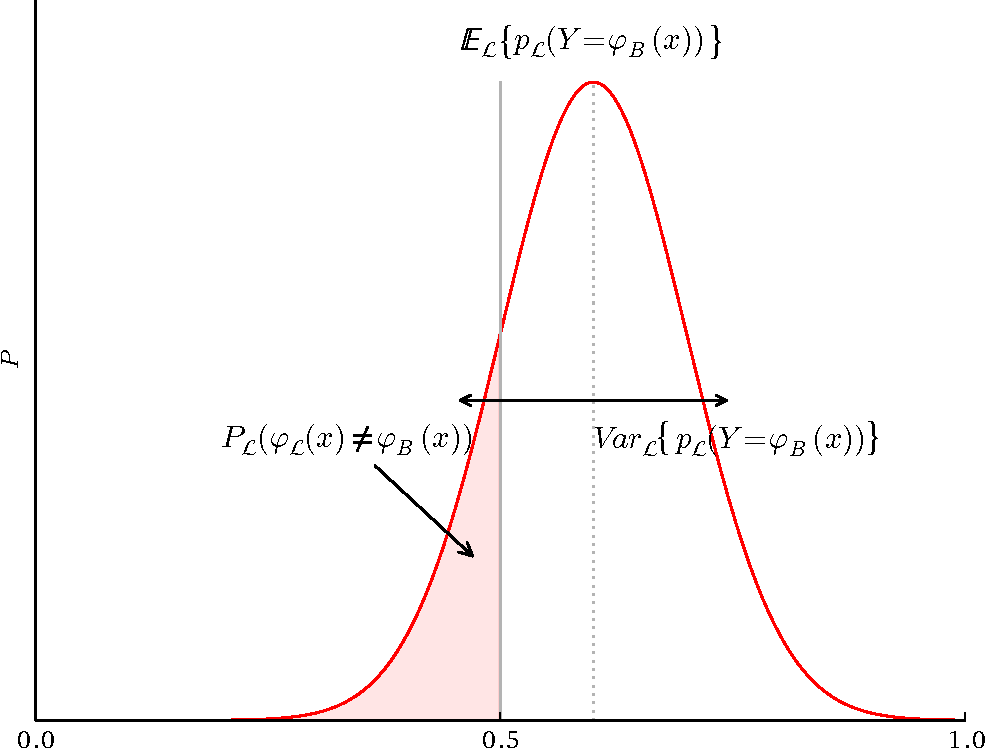
\includegraphics[width=0.9\textwidth]{figures/ch4_estimate_distribution.pdf}
    \caption{Probability distribution of the estimate $\widehat{p}_{\cal L}(Y=\varphi_B(\mathbf{x}))$.}
    \label{fig:estimate-distribution}
\end{figure}

If we now further assume\footnote{For single decision trees, the normal
assumption is certainly not satisfied in all cases, but the qualitative
conclusions are still generally valid. When the computations of the estimates
involve some averaging process, e.g., as further developed in the case of
ensemble of randomized trees, this approximation is however fairly reasonable.}
that the estimate $\widehat{p}_{\cal L}(Y=\varphi_B(\mathbf{x}))$ is normally distributed,
then probability~\ref{eqn:4:prob-diff-from-bayes} can be computed explicitly
from its mean and variance:
\begin{equation}
P_{\cal L}(\widehat{p}_{\cal L}(Y=\varphi_B(\mathbf{x})) < 0.5) = \Phi(\frac{0.5 - \mathbb{E}_{\cal L}\{ \widehat{p}_{\cal L}(Y=\varphi_B(\mathbf{x})) \}}{\sqrt{\mathbb{V}_{\cal L}\{ \widehat{p}_{\cal L}(Y=\varphi_B(\mathbf{x})) \}}})
\end{equation}
where $\Phi(x)=\frac{1}{\sqrt{2\pi}} \int_{-\infty}^x \exp(-\frac{t^2}{2}) dt$
is the cumulative distribution function of the standard normal distribution.
In summary, the expected generalization error additively
decomposes as formulated in Theorem~\ref{thm:bias-variance:classification}.

\begin{theorem}\label{thm:bias-variance:classification}
For the zero-one loss and binary classification, the expected
generalization error $\mathbb{E}_{\cal L} \{ Err(\varphi_{\cal L}(\mathbf{x}))
\}$ at $X=\mathbf{x}$ decomposes as follows:

\begin{align}
\mathbb{E}_{\cal L} \{ Err(\varphi_{\cal L}(\mathbf{x})) \} &= P(\varphi_B(\mathbf{x})\neq Y) \\
                                                            &+ \Phi(\frac{0.5 - \mathbb{E}_{\cal L}\{ \widehat{p}_{\cal L}(Y=\varphi_B(\mathbf{x})) \}}{\sqrt{\mathbb{V}_{\cal L}\{ \widehat{p}_{\cal L}(Y=\varphi_B(\mathbf{x})) \}}}) (2 P(\varphi_B(\mathbf{x}) = Y) - 1) \nonumber
\end{align}
\end{theorem}

As a result, Theorem~\ref{thm:bias-variance:classification} establishes a
direct connection between the regression variance of the estimates and the
classification error of the resulting model. In practice, this decomposition
has important consequences:
\begin{itemize}
\item When the expected probability estimate $\mathbb{E}_{\cal L}\{ \widehat{p}_{\cal L}(Y=\varphi_B(\mathbf{x}) \}$
      for the true majority class is greater than $0.5$, a reduction of
      variance of the estimate results in a decrease of the total misclassification
      error. If $\mathbb{V}_{\cal L}\{ \widehat{p}_{\cal L}(Y=\varphi_B(\mathbf{x})) \} \to 0$,
      then $\Phi \to 0$ and the expected generalization error tends to the error of the Bayes model.
      In particular, the generalization error can be driven to its minimum
      value whatever the regression bias of the estimate (at least as long as $\mathbb{E}_{\cal L}\{ \widehat{p}_{\cal L}(Y=\varphi_B(\mathbf{x}) \} > 0.5$).
\item Conversely, when $\mathbb{E}_{\cal L}\{ \widehat{p}_{\cal L}(Y=\varphi_B(\mathbf{x}) \} < 0.5$,
      a decrease of variance might actually increase the total misclassification error.
      If $\mathbb{V}_{\cal L}\{ \widehat{p}_{\cal L}(Y=\varphi_B(\mathbf{x})) \} \to 0$,
      then $\Phi \to 1$ and the error is maximal.
\end{itemize}


\section{Ensemble methods based on randomization}
\label{sec:4:ensemble}

Both theorems~\ref{thm:bias-variance} and \ref{thm:bias-variance:classification}
reveal the role of variance in the expected generalization error of a model. In
light of these results, a sensible approach for reducing generalization error
would therefore consist in driving down the prediction variance, provided the
respective bias can be kept the same or not be increased too much.

As it happens, \textit{ensemble methods} constitute a beautifully simple way to
do just that. Specifically, the core principle of ensemble methods based on randomization is to
introduce random perturbations into the learning procedure in order to produce
several different models from a single learning set ${\cal L}$ and then to
combine the predictions of those models to form the prediction of the ensemble.
How predictions are combined and why does it help is formally studied in the
next sections.


\subsection{Randomized models}

Given a learning set ${\cal L}$, a learning algorithm ${\cal A}$
deterministically produces a model ${\cal A}(\theta, {\cal L})$, denoted
$\varphi_{{\cal L},\theta}$\label{ntn:varphi-Ltheta}, where $\theta$ are
hyper-parameters controlling the execution of ${\cal A}$. Let us assume that $\theta$
includes a random seed parameter for mimicking some stochastic behavior in
${\cal A}$, hence producing (pseudo-)randomized models that are more or less
different from one random seed to another. (We defer the discussion on specific
random perturbations in the case of decision trees to Section~\ref{sec:4:random-forests}.)

In this context, the bias-variance decomposition can be extended to account for
everything that is random, hence considering both ${\cal L}$ and $\theta$ as
random variables\footnote{From now on, and without loss of generality, we
assume that the random variable $\theta$ only controls the randomness of the
learning algorithm.}.
Accordingly, theorems~\ref{thm:bias-variance} and \ref{thm:bias-variance:classification}
naturally extend to the expected generalization error
$\mathbb{E}_{{\cal L},\theta} \{ Err(\varphi_{{\cal L},\theta}(\mathbf{x})) \}$
of the randomized model $\varphi_{{\cal L},\theta}$ by replacing expectations
$\mathbb{E}_{\cal L} \{ . \}$ and variances $\mathbb{V}_{\cal L} \{ . \}$ with
their respective counterparts $\mathbb{E}_{{\cal L},\theta} \{ . \}$ and
$\mathbb{V}_{{\cal L},\theta} \{ . \}$ computed over the joint distribution of
${\cal L}$ and $\theta$. In regression, the bias-variance decomposition
of the squared error loss thus becomes:
\begin{equation}
\mathbb{E}_{{\cal L},\theta} \{ Err(\varphi_{{\cal L},\theta}(\mathbf{x})) \} = \text{noise}(\mathbf{x}) + \text{bias}^2(\mathbf{x}) + \text{var}(\mathbf{x}),
\end{equation}
where
\begin{align}
\text{noise}(\mathbf{x}) &= Err(\varphi_B(\mathbf{x})), \\
\text{bias}^2(\mathbf{x}) &= (\varphi_B(\mathbf{x}) - \mathbb{E}_{{\cal L},\theta} \{ \varphi_{{\cal L},\theta}(\mathbf{x}) \} )^2, \\
\text{var}(\mathbf{x}) &= \mathbb{E}_{{\cal L},\theta} \{ (\mathbb{E}_{{\cal L},\theta} \{ \varphi_{{\cal L},\theta}(\mathbf{x}) \} - \varphi_{{\cal L},\theta}(\mathbf{x}))^2 \}.
\end{align}

In this form, variance now accounts for both the prediction variability due to
the randomness of the learning set ${\cal L}$ and the variability due to the
randomness of the learning algorithm itself. As such, the variance of a
randomized algorithm is typically larger than the variance of its
deterministic counterpart. Depending on the strength of randomization, bias
also usually increases, but often to a smaller extent than variance.

While randomizing an algorithm might seem counter-intuitive, since it
increases both variance and bias, we will show in Section~\ref{sec:4:bias-variance:ensemble}
that combining several such randomized models might actually
achieve better performance than a single non-randomized model.


\subsection{Combining randomized models}

Let us assume a set of $M$\label{ntn:M} randomized models $\{\varphi_{{\cal L}, \theta_m} |
m = 1, \dots, M \}$, all learned on the same data ${\cal L}$ but each built
from an independent random seed $\theta_m$\label{ntn:theta-seed}\label{ntn:theta-seed-m}. Ensemble methods work by combining
the predictions of these models into a new \textit{ensemble} model, denoted
$\psi_{{\cal L},\theta_1,\dots,\theta_M}$\label{ntn:psi}, such that the expected
generalization error of the ensemble is (hopefully) smaller than the expected
generalization error of the individual randomized models.

In regression, for the squared error loss, the most common way to combine the
randomized models into an ensemble is to average their predictions to form the
final prediction:
\begin{equation}\label{eqn:4:averaging}
\psi_{{\cal L},\theta_1,\dots,\theta_M}(\mathbf{x}) = \frac{1}{M} \sum_{m=1}^M \varphi_{{\cal L},\theta_m}(\mathbf{x})
\end{equation}
The rationale is that the average prediction is the prediction that minimizes the average
squared error with respect to the individual predictions of the models. In that sense, the average prediction is the closest prediction with respect to all individual predictions.

\begin{remark}{Ambiguity decomposition}
For prediction averaging, as defined in Equation~\ref{eqn:4:averaging},
the \textit{ambiguity decomposition}~\citep{krogh:1995}
guarantees the generalization error of the ensemble to be lower
than the average generalization error of its constituents. Formally,
the ambiguity decomposition states that
\begin{equation}
Err(\psi_{{\cal L},\theta_1,\dots,\theta_M}) = \overline{E} - \overline{A}
\end{equation}
where
\begin{align}
\overline{E} &= \frac{1}{M} \sum_{m=1}^M Err(\varphi_{{\cal L},\theta_m}), \\
\overline{A} &= \mathbb{E}_{X} \{ \frac{1}{M} \sum_{m=1}^M (\varphi_{{\cal L},\theta_m}(X) - \psi_{{\cal L},\theta_1,\dots,\theta_M}(X))^2 \}.
\end{align}
The first term is the average generalization error of the individual models. The second term is the ensemble ambiguity and
corresponds to the variance of the individual predictions around the prediction of the ensemble. Since $\overline{A}$ is non-negative,
the generalization error of the ensemble is therefore smaller than the average generalization
error of its constituents.
\end{remark}

In classification, for the zero-one loss, predictions are usually aggregated by considering the
models in the ensemble as a committee  and then resorting to \textit{majority voting} to
form the final prediction:
\begin{equation}\label{eqn:4:majority-vote}
\psi_{{\cal L},\theta_1,\dots,\theta_M}(\mathbf{x}) = \argmax_{c \in {\cal Y}}  \sum_{m=1}^M 1(\varphi_{{\cal L},\theta_m}(\mathbf{x})=c)
\end{equation}
Similarly, the rationale is that the majority prediction is the prediction that minimizes
the average zero-one error with respect to the individual predictions.
Alternatively, when individual models provide class probability estimates $\widehat{p}_{{\cal L},\theta m}(Y=c|X=\mathbf{x})$,
\textit{soft voting}~\citep{zhou:2012}
consists in averaging the class probability estimates
and then predict the class which is the most likely:
\begin{equation}\label{eqn:4:avg-estimate}
\psi_{{\cal L},\theta_1,\dots,\theta_M}(\mathbf{x}) = \argmax_{c \in {\cal Y}} \frac{1}{M} \sum_{m=1}^M \widehat{p}_{{\cal L},\theta m}(Y=c|X=\mathbf{x})
\end{equation}
As empirically investigated by \citet{breiman:1996b}, both approaches yield
results that are nearly identical\footnote{In the case of ensembles of fully developed decision trees that perfectly classify all samples from ${\cal L}$, majority voting and soft voting are exactly equivalent.}. From a practical point of view however,
Equation~\ref{eqn:4:avg-estimate} has the advantage of providing accurate class
probability estimates for the ensemble, which may prove to be useful in
critical applications, e.g., when (estimates of) the certainty about
predictions is as important as the predictions themselves. Additionally,
combining predictions in this way makes it easy to study the expected
generalization error of the ensemble -- it suffices to plug the averaged
estimates into Theorem~\ref{thm:bias-variance:classification}. For these
reasons, and for the rest of this work, predictions in classification are now
assumed to be combined with soft voting (see Equation~\ref{eqn:4:avg-estimate}) unless
mentioned otherwise.

\begin{remark}{Condorcet's jury theorem}
Majority voting, as defined in Equation~\ref{eqn:4:majority-vote},
finds its origins in the \textit{Condorcet's jury theorem}
from the field of political science. Let consider a group of $M$ voters that
wishes to reach a decision by majority vote. The theorem states that if each
voter has an independent  probability $p > \tfrac{1}{2}$ of voting for the
correct decision, then adding more voters increases the probability of
the majority decision to be correct. When $M \to \infty$, the probability that the decision
taken by the group is correct approaches $1$. Conversely, if $p < \tfrac{1}{2}$, then
each voter is more likely to vote incorrectly and increasing $M$ makes things
worse.
\end{remark}

\subsection{Bias-variance decomposition of an ensemble}
\label{sec:4:bias-variance:ensemble}

Let us now study the bias-variance decomposition of the expected generalization
error of an ensemble $\psi_{{\cal L},\theta_1,\dots,\theta_M}$, first in the
case in case of regression and then for classification.

To simplify notations in the analysis below, let us denote the mean prediction at
$X=\mathbf{x}$ of a single randomized model $\varphi_{{\cal L},\theta_m}$ and its
respective prediction variance as:
\begin{align}
\mu_{{\cal L},\theta_m}(\mathbf{x}) &= \mathbb{E}_{{\cal L},\theta_m} \{ \varphi_{{\cal L},\theta_m}(\mathbf{x}) \} \label{eqn:4:mu} \\
\sigma^2_{{\cal L},\theta_m}(\mathbf{x}) &= \mathbb{V}_{{\cal L},\theta_m} \{ \varphi_{{\cal L},\theta_m}(\mathbf{x}) \label{eqn:4:sigma} \}
\end{align}

\subsubsection{Regression}

From Theorem~\ref{thm:bias-variance}, the expected generalization error of an
ensemble $\psi_{{\cal L},\theta_1,\dots,\theta_M}$ made of $M$ randomized
models decomposes into a sum of $\text{noise}(\mathbf{x})$,
$\text{bias}^2(\mathbf{x})$ and $\text{var}(\mathbf{x})$ terms.

The noise term only depends on the intrinsic randomness of $Y$. Its value
stays therefore the same, no matter the learning algorithm:
\begin{equation}
\text{noise}(\mathbf{x}) = \mathbb{E}_{Y|X=\mathbf{x}} \{ (Y - \varphi_B(\mathbf{x}))^2 \}
\end{equation}

The (squared) bias term is the (squared) difference between the prediction of the Bayes model
and the average prediction of the model. For an ensemble, the average prediction
is in fact the same as the average prediction of the corresponding randomized individual model. Indeed,
\begin{align}
\mathbb{E}_{{\cal L},\theta_1,\dots,\theta_M} \{ \psi_{{\cal L},\theta_1,\dots,\theta_M}(\mathbf{x}) \} &= \mathbb{E}_{{\cal L},\theta_1,\dots,\theta_M} \{ \frac{1}{M} \sum_{m=1}^M \varphi_{{\cal L},\theta_m}(\mathbf{x}) \} \nonumber \\
&= \frac{1}{M} \sum_{m=1}^M \mathbb{E}_{{\cal L},\theta_m} \{ \varphi_{{\cal L},\theta_m}(\mathbf{x}) \} \nonumber \\
&= \mu_{{\cal L},\theta}(\mathbf{x})
\end{align}
since random variables $\theta_m$ are independent and all follow the
same distribution. As a result,
\begin{equation}
\text{bias}^2(\mathbf{x}) = (\varphi_B(\mathbf{x}) - \mu_{{\cal L},\theta}(\mathbf{x}))^2,
\end{equation}
which indicates that the bias of an ensemble of randomized models is the same
as the bias of any of the randomized models. Put otherwise, combining
randomized models has no effect on the bias of the resulting ensemble.

On variance on the other hand, ensemble methods show all their raison d'etre,
virtually reducing the variability of predictions to almost nothing and thereby
improving the accuracy of the ensemble. Before considering the variance of
$\psi_{{\cal L},\theta_1,\dots,\theta_M}(\mathbf{x})$ however, let us first
derive the correlation coefficient $\rho(\mathbf{x})$ between the predictions
of two randomized models built on the same learning set, but grown from two
independent random seeds $\theta^\prime$ and $\theta^{\prime\prime}$. From the definition of the Pearson's correlation
coefficient, it comes:
\begin{align}
\rho(\mathbf{x}) &= \frac{\mathbb{E}_{{\cal L},\theta^\prime,\theta^{\prime\prime}} \{ (\varphi_{{\cal L}, \theta^\prime}(\mathbf{x}) - \mu_{{\cal L},\theta^\prime}(\mathbf{x})) (\varphi_{{\cal L}, \theta^{\prime\prime}}(\mathbf{x}) - \mu_{{\cal L},\theta^{\prime\prime}}(\mathbf{x})) \}}{\sigma_{{\cal L},\theta^\prime}(\mathbf{x}) \sigma_{{\cal L},\theta^{\prime\prime}}(\mathbf{x})} \nonumber \\
&= \frac{\mathbb{E}_{{\cal L},\theta^\prime,\theta^{\prime\prime}} \{ \varphi_{{\cal L},\theta^\prime}(\mathbf{x}) \varphi_{{\cal L},\theta^{\prime\prime}}(\mathbf{x}) - \varphi_{{\cal L},\theta^\prime}(\mathbf{x}) \mu_{{\cal L},\theta^{\prime\prime}}(\mathbf{x}) - \varphi_{{\cal L},\theta^{\prime\prime}}(\mathbf{x}) \mu_{{\cal L},\theta^\prime}(\mathbf{x}) + \mu_{{\cal L},\theta^\prime}(\mathbf{x}) \mu_{{\cal L},\theta^{\prime\prime}}(\mathbf{x}) \}}{\sigma^2_{{\cal L},\theta}(\mathbf{x})} \nonumber \\
&= \frac{\mathbb{E}_{{\cal L},\theta^\prime,\theta^{\prime\prime}} \{ \varphi_{{\cal L},\theta^\prime}(\mathbf{x}) \varphi_{{\cal L},\theta^{\prime\prime}}(\mathbf{x}) \} - \mu^2_{{\cal L},\theta}(\mathbf{x})}{\sigma^2_{{\cal L},\theta}(\mathbf{x})} \label{eqn:4:correlation}
\end{align}
since random variables $\theta^\prime$ and $\theta^{\prime\prime}$ follow the same
distribution. Intuitively, $\rho(\mathbf{x})$ represents the strength of the
random perturbations introduced in the learning algorithm. When it is close to
$1$, predictions of two randomized models are highly correlated, suggesting
that randomization has no sensible effect on the predictions. By contrast, when
it is close to $0$, predictions of the randomized models are decorrelated,
hence indicating that randomization has a strong effect on the predictions. At
the limit, when $\rho(\mathbf{x})=0$, predictions of two models built on the
same learning set ${\cal L}$ are independent, which happens when they are
perfectly random.

From Equation~\ref{eqn:4:correlation}, the variance of $\psi_{{\cal
L},\theta_1,\dots,\theta_M}(\mathbf{x})$ can now be derived as follows:
\begin{align}
\text{var}(\mathbf{x}) &= \mathbb{V}_{{\cal L},\theta_1,\dots,\theta_M} \{ \frac{1}{M} \sum_{m=1}^M \varphi_{{\cal L},\theta_m}(\mathbf{x})  \} \nonumber \\
&= \frac{1}{M^2} \Bigg[ \mathbb{E}_{{\cal L},\theta_1,\dots,\theta_M} \{ (\sum_{m=1}^M \varphi_{{\cal L},\theta_m}(\mathbf{x}))^2 \} - \mathbb{E}_{{\cal L},\theta_1,\dots,\theta_M} \{ \sum_{m=1}^M \varphi_{{\cal L},\theta_m}(\mathbf{x}) \}^2 \Bigg] \nonumber \\
&= \frac{1}{M^2} \Bigg[ \mathbb{E}_{{\cal L},\theta_1,\dots,\theta_M} \{ \sum_{i,j} \varphi_{{\cal L},\theta_i}(\mathbf{x}) \varphi_{{\cal L},\theta_j}(\mathbf{x}) \} - (M \mu_{{\cal L},\theta}(\mathbf{x}))^2 \Bigg] \nonumber \\
&= \frac{1}{M^2} \Bigg[ \sum_{i,j} \mathbb{E}_{{\cal L},\theta_i,\theta_j} \{  \varphi_{{\cal L},\theta_i}(\mathbf{x}) \varphi_{{\cal L},\theta_j}(\mathbf{x}) \} - M^2 \mu^2_{{\cal L},\theta}(\mathbf{x}) \Bigg] \nonumber \\
&= \frac{1}{M^2} \Bigg[ M \mathbb{E}_{{\cal L},\theta} \{ \varphi_{{\cal L},\theta}(\mathbf{x})^2 \} \nonumber \\
&\quad \hookrightarrow + (M^2-M) \mathbb{E}_{{\cal L},\theta^\prime,\theta^{\prime\prime}} \{  \varphi_{{\cal L},\theta^\prime}(\mathbf{x}) \varphi_{{\cal L},\theta^{\prime\prime}}(\mathbf{x}) \}  - M^2 \mu^2_{{\cal L},\theta}(\mathbf{x}) \Bigg] \nonumber \\
&= \frac{1}{M^2} \Bigg[ M (\sigma^2_{{\cal L},\theta}(\mathbf{x}) + \mu^2_{{\cal L},\theta}(\mathbf{x})) \nonumber \\
&\quad \hookrightarrow + (M^2-M)(\rho(\mathbf{x}) \sigma^2_{{\cal L},\theta}(\mathbf{x}) + \mu^2_{{\cal L},\theta}(\mathbf{x})) - M^2 \mu^2_{{\cal L},\theta}(\mathbf{x}) \Bigg] \nonumber \\
&= \frac{\sigma^2_{{\cal L},\theta}(\mathbf{x})}{M} + \rho(\mathbf{x})\sigma^2_{{\cal L},\theta}(\mathbf{x}) - \rho(\mathbf{x}) \frac{\sigma^2_{{\cal L},\theta}(\mathbf{x})}{M} \nonumber \\
&= \rho(\mathbf{x}) \sigma^2_{{\cal L},\theta}(\mathbf{x}) + \frac{1 - \rho(\mathbf{x})}{M} \sigma^2_{{\cal L},\theta}(\mathbf{x}) \label{eqn:4:variance-hastie}
\end{align}
As the size of the ensemble gets arbitrarily large, i.e., as $M \to \infty$,
the variance of the ensemble reduces to $\rho(\mathbf{x})
\sigma^2_{{\cal L},\theta}(\mathbf{x})$. Under the assumption that randomization has some
effect on the predictions of randomized models, i.e., assuming
$\rho(\mathbf{x}) < 1$, the variance of an ensemble is therefore strictly
smaller than the variance of an individual model. As a result, the expected
generalization error of an ensemble is strictly smaller than the expected error
of a randomized model. As such, improvements in predictions are
solely the result of variance reduction, since both $\text{noise}(\mathbf{x})$
and $\text{bias}^2(\mathbf{x})$ remain unchanged. Additionally, when random
effects are strong, i.e., when $\rho(\mathbf{x}) \to 0$, variance reduces to
$\smash{\tfrac{\sigma^2_{{\cal L},\theta}(\mathbf{x})}{M}}$, which can further be driven to $0$ by
increasing the size of the ensemble. On the other hand, when random effects are weak,
i.e., when $\rho(\mathbf{x}) \to 1$, then variance reduces to $\sigma^2_{{\cal
L},\theta}(\mathbf{x})$ and building an ensemble brings no benefit. Put otherwise, the stronger the random effects, the larger
the reduction of variance due to ensembling, and vice-versa.

In summary, the expected generalization error of an ensemble additively
decomposes as stated in Theorem~\ref{thm:bias-variance:ensemble}.
\begin{theorem}\label{thm:bias-variance:ensemble}
For the squared error loss, the bias-variance decomposition of the expected
generalization error $\mathbb{E}_{\cal L} \{ Err( \psi_{{\cal L},\theta_1,\dots,\theta_M}(\mathbf{x}))
\}$ at $X=\mathbf{x}$ of an ensemble of $M$ randomized models $\varphi_{{\cal L},\theta_m}$ is
\begin{equation}
\mathbb{E}_{\cal L} \{ Err(\psi_{{\cal L},\theta_1,\dots,\theta_M}(\mathbf{x})) \} = \text{noise}(\mathbf{x}) + \text{bias}^2(\mathbf{x}) + \text{var}(\mathbf{x}),
\end{equation}
where
\begin{align*}
\text{noise}(\mathbf{x}) &= Err(\varphi_B(\mathbf{x})), \\
\text{bias}^2(\mathbf{x}) &= (\varphi_B(\mathbf{x}) - \mathbb{E}_{{\cal L},\theta} \{ \varphi_{{\cal L},\theta}(\mathbf{x}) \} )^2, \\
\text{var}(\mathbf{x}) &= \rho(\mathbf{x}) \sigma^2_{{\cal L},\theta}(\mathbf{x}) + \frac{1 - \rho(\mathbf{x})}{M} \sigma^2_{{\cal L},\theta}(\mathbf{x}).
\end{align*}
\end{theorem}

In light of Theorem~\ref{thm:bias-variance:ensemble}, the core principle of
ensemble methods is thus to introduce random perturbations in order to
decorrelate as much as possible the predictions of the individual models,
thereby maximizing variance reduction. However, random perturbations need to be
carefully chosen so as to increase bias as little as possible.  The crux of the
problem is to find the right trade-off between randomness and bias.

\begin{remark}{Alternative variance decomposition}
\citet{geurts:2002} alternatively decomposes the ensemble variance as
\begin{equation}\label{eqn:4:variance-geurts}
\text{var}(\mathbf{x}) = \mathbb{V}_{\cal L} \{ \mathbb{E}_{\theta|{\cal L}} \{ \varphi_{{\cal L},\theta}(\mathbf{x}) \} \} + \frac{1}{M} \mathbb{E}_{\cal L} \{ \mathbb{V}_{\theta|{\cal L}} \{ \varphi_{{\cal L},\theta}(\mathbf{x}) \} \}.
\end{equation}
The first term of this decomposition is the variance due to the randomness
of the learning set ${\cal L}$, averaged over the random perturbations due to $\theta$. It
measures the dependence of the model on the learning set, independently of
$\theta$. The second term is the expectation over all learning sets of
the variance with respect to $\theta$. It measures the strength of the
random effects. As the decomposition shows, only this last part of the variance
can be reduced as a result of averaging, which is consistent with our previous
conclusions.  The stronger the random effects, the larger the variance with
respect to $\theta$, and hence the larger of reduction of variance due
to ensembling.

Decompositions \ref{eqn:4:variance-hastie} and \ref{eqn:4:variance-geurts} are equivalent if Equation~\ref{eqn:4:correlation}
is equivalent to
\begin{equation}\label{eqn:4:correlation-bis}
\rho(\mathbf{x}) = \frac{\mathbb{V}_{\cal L} \{ \mathbb{E}_{\theta|{\cal L}} \{ \varphi_{{\cal L},\theta}(\mathbf{x}) \} \}}{\mathbb{V}_{\cal L} \{ \mathbb{E}_{\theta|{\cal L}} \{ \varphi_{{\cal L},\theta}(\mathbf{x}) \} \} + \mathbb{E}_{\cal L} \{ \mathbb{V}_{\theta|{\cal L}} \{ \varphi_{{\cal L},\theta}(\mathbf{x}) \} \}}.
\end{equation}
From the law of total variance, the denominator of Equation~\ref{eqn:4:correlation} expands
to the denominator of Equation~\ref{eqn:4:correlation-bis}:
\begin{equation}
\sigma^2_{{\cal L},\theta}(\mathbf{x}) = \mathbb{V}_{\cal L} \{ \mathbb{E}_{\theta|{\cal L}} \{ \varphi_{{\cal L},\theta}(\mathbf{x}) \} \} + \mathbb{E}_{\cal L} \{ \mathbb{V}_{\theta|{\cal L}} \{ \varphi_{{\cal L},\theta}(\mathbf{x}) \} \}
\end{equation}
Similarly, the numerator of Equation~\ref{eqn:4:correlation-bis} can be reexpressed
as the numerator of Equation~\ref{eqn:4:correlation}, thereby proving the equivalence:
\begin{align}
& \mathbb{V}_{\cal L} \{ \mathbb{E}_{\theta|{\cal L}} \{ \varphi_{{\cal L},\theta}(\mathbf{x}) \} \} \nonumber \\
&= \mathbb{E}_{\cal L} \{ (\mathbb{E}_{\theta|{\cal L}} \{ \varphi_{{\cal L},\theta}(\mathbf{x}) \} - \mathbb{E}_{\cal L} \{ \mathbb{E}_{\theta|{\cal L}} \{ \varphi_{{\cal L},\theta}(\mathbf{x})\} \})^2 \} \nonumber \\
&= \mathbb{E}_{\cal L} \{ (\mathbb{E}_{\theta|{\cal L}} \{ \varphi_{{\cal L},\theta}(\mathbf{x}) \} - \mu_{{\cal L},\theta}(\mathbf{x}))^2 \} \nonumber \\
&= \mathbb{E}_{\cal L} \{ \mathbb{E}_{\theta|{\cal L}} \{ \varphi_{{\cal L},\theta}(\mathbf{x}) \}^2 \} - \mu^2_{{\cal L},\theta}(\mathbf{x}) \nonumber \\
&= \mathbb{E}_{\cal L} \{ \mathbb{E}_{\theta^\prime|{\cal L}} \{ \varphi_{{\cal L},\theta^\prime}(\mathbf{x}) \} \mathbb{E}_{\theta^{\prime\prime}|{\cal L}} \{ \varphi_{{\cal L},\theta^{\prime\prime}}(\mathbf{x}) \} \} - \mu^2_{{\cal L},\theta}(\mathbf{x}) \nonumber \\
&= \mathbb{E}_{{\cal L},\theta^\prime,\theta^{\prime\prime}} \{ \varphi_{{\cal L},\theta^\prime}(\mathbf{x}) \varphi_{{\cal L},\theta^{\prime\prime}}(\mathbf{x}) \} - \mu^2_{{\cal L},\theta}(\mathbf{x}).
\end{align}
In this form, $\rho(\mathbf{x})$ is interpreted as the ratio between the variance
due to the learning set  and the total variance, accounting for
random effects due to both the learning set and the random perturbations.
It is close to $1$ when variance is mostly due to the learning set, hence
yielding correlated predictions. Conversely, it is close to $0$ when variance
is mostly due to the random perturbations induced by $\theta$, hence decorrelating
the predictions.
\end{remark}

\subsubsection{Classification}

The decomposition of the expected generalization error of an ensemble in
classification directly follows from theorems~\ref{thm:bias-variance:classification} and
\ref{thm:bias-variance:ensemble}.
Building an ensemble always reduces the variance of the class probability estimate
$\mathbb{E}_{{\cal L},\theta}\{ \widehat{p}_{{\cal
L},\theta}(Y=\varphi_B(\mathbf{x}) \}$ (as shown in Equation~\ref{eqn:4:variance-hastie}), which results in a decrease of the misclassification error
if the expected estimate remains strictly greater than $0.5$ in a
randomized model.

\begin{remark}{Shortcomings addressed by ensembles}
In complement with the formal bias-variance analysis carried out in the previous
section, \citet{dietterich:2000b} identifies three fundamental reasons
intuitively explaining why ensembles often work better than single models.

The first reason is statistical. When the learning set is too small, a learning
algorithm can typically find several models in the hypothesis space ${\cal H}$
that all give the same performance on the training data. Provided their predictions
are uncorrelated, averaging several models reduces the risk of choosing the wrong hypothesis.

The second reason is computational. Many learning algorithms rely on some
greedy assumption or local search that may get stuck in local optima. As such, an ensemble
made of individual models built from many different starting points may provide
a better approximation of the true unknown function that any of the single
models.

Finally, the third reason is representational. In most cases, for a learning set of finite size, the true
function cannot be represented by any of the candidate models in ${\cal H}$.
By combining several models in an ensemble, it may be possible to expand the space
of representable functions and to better model the true function.
\end{remark}


\section{Random Forests}
\label{sec:4:random-forests}

Random forests\footnote{The term
\textit{random forests}, without capitals, is used to denote any ensemble of decision
trees. Specific variants are referred to using their original designation,
denoted with capitals. In particular, the ensemble method due to
\citet{breiman:2001} is denoted as \textit{Random Forests}, with capitals.}
form a family of methods that consist in building an ensemble (or
\textit{forest}) of decision trees grown from a randomized variant of the tree
induction algorithm (as described in Chapter~\ref{ch:cart}). Decision trees are
indeed ideal candidates for ensemble methods since they usually have low bias
and high variance, making them very likely to benefit from the averaging
process. As we will review in this section, random forests methods mostly
differ from each other in the way they introduce random perturbations into the
induction procedure. As highlighted in the previous section, the difficulty is
to inject randomness while minimizing $\rho(\mathbf{x})$ and
simultaneously maintaining a low bias in the randomized decision trees.

\subsection{Randomized induction algorithms}

\begin{description}

\item \citet{kwok:1990}: \hfill \\
    Historically, the earliest mention of ensemble of decision trees is due to
    \citet{kwok:1990}. In this work, the authors empirically observe that
    averaging multiple decision trees with different structure consistently
    produce better results than any of the constituents of the ensemble. This
    approach however was not based on randomization nor was fully automatic:
    decision trees were generated by first manually selecting at the top of the
    tree splits that were almost as good as the optimal splits, and then
    expanded using the classical ID3 induction procedure.

\item \citet{breiman:1996b}: \hfill \\
    In a now famous technical report, \citet{breiman:1996b} was one of the earliest to
    show, both theoretically and empirically, that aggregating multiple
    versions of an estimator into an ensemble can give substantial gains in
    accuracy. He notes and shows that the average model $\mathbb{E}_{\cal L}\{
    \varphi_{\cal L} \}$ has a lower expected generalization error than
    $\varphi_{\cal L}$. As such, \textit{Bagging}  consists in
    approximating $\mathbb{E}_{\cal L}\{ \varphi_{\cal L} \}$  by combining
    models built from \textit{bootstrap samples}~\citep{efron:1979} ${\cal
    L}^m$\label{ntn:L_m} (for $m=1,\dots,M$) of the learning set ${\cal L}$. The $\{ {\cal
    L}^m \}$ form replicates of ${\cal L}$, each consisting of $N$ cases $(\mathbf{x},y)$, drawn
    at random but \textit{with replacement} from ${\cal L}$.

    Note that even
    though $|{\cal L}|=|{\cal L}^m|=N$, $37\%$ of the couples $(\mathbf{x},y)$ from ${\cal L}$
    are on average missing in the bootstrap replicates. Indeed, after $N$ draws
    with replacement, the probability of never have been selected is
    \begin{equation}
    (1 - \frac{1}{N})^N \approx \frac{1}{e} \approx 0.368.
    \end{equation}
    When the learning algorithm is unstable (i.e., when small changes in the
    learning set can cause large changes in the learned models), Bagging
    generates individual models that are  different from one bootstrap sample
    to another, hence making them likely to benefit from the averaging process.
    In some cases however, when the learning set ${\cal L}$ is small,
    subsampling $67\%$ of the objects might lead to an increase of bias which
    is too large to be compensated by a decrease of variance, hence resulting
    in overall poorer performance. Despite this defect, Bagging has proven to
    be an effective method in numerous applications, one of its strengths being
    that it can be used to combine any kind of models -- i.e., not only
    decision trees.

\item \citet{dietterich:1995}: \hfill \\
    Building upon \citep{kwok:1990}, \citet{dietterich:1995} propose
    to randomize the choice of the best split at a given node by selecting
    uniformly at random one of the $20$ best splits of node $t$. The authors empirically
    show in \citep{dietterich:1995,dietterich:2000} that randomizing in this
    way gives results that are slightly better than Bagging in low noise settings.
    Experiments show however that when noise is important, Bagging usually
    yield better results. From a bias-variance point of view, this method
    virtually does not change bias but increases variance due to randomization.

\item \citet{amit:1997}: \hfill \\
    In the context of handwritten character recognition, where the number $p$
    of input variables is typically very large, \citet{amit:1997} propose a
    randomized variant of the tree induction algorithm that consists in
    searching for the best split at each node over a random subsample of the
    variables.

    Denoting $K \leq p$\label{ntn:K-split} (also known as \texttt{mtry} or
    \texttt{max\_features}) the number of variables effectively considered at
    each node, this variant replaces Algorithm~\ref{algo:findsplit}
    with the following randomized alternative:
    \begin{algorithm}\label{algo:findsplit:random}
    Find the best split $s^*$ that partitions ${\cal L}_t$, among a random subset of $K \leq p$ input variables.
    \textnormal{
    \begin{algorithmic}[1]
    \Function{FindBestSplitRandom}{${\cal L}_t$, $K$}
        \State $\Delta = -\infty$
        \State Draw $K$ random indices $j_k$ from $1,\dots,p$
        \For{$k=1, \dots, K$}
            \State Find the best binary split $s^*_{j_k}$ defined on $X_{j_k}$
            \If{$\Delta i(s^*_{j_k}, t) > \Delta$}
                \State $\Delta = \Delta i(s^*_{j_k}, t)$
                \State $s^* = s^*_{j_k}$
            \EndIf
        \EndFor
        \State \Return $s^*$
    \EndFunction
    \end{algorithmic}
    }
    \end{algorithm}
    When the output $Y$ can be explained in several ways, this randomized
    algorithm generates trees that are each structurally different, yet
    individually good. As a result, bias usually increases only slightly, while
    the increased variance due to randomization can be cancelled out through averaging. The
    optimal trade-off between these quantities can otherwise be adjusted by
    tuning the value of $K$. As $K \to 1$, the larger the bias but the larger the
    variance of the individual models and hence the more effective the
    averaging process. Conversely, as $K \to p$, the smaller the bias but also the
    smaller the variance of the individual models and therefore the less
    beneficial the ensemble.

\item \citet{ho:1998}: \hfill \\
    Inspired from the principles of Bagging~\citep{breiman:1996b} and
    random subsets of variables~\citep{amit:1997}, \citet{ho:1998} proposes
    with the \textit{Random Subspace} (RS) method to build a \textit{decision
    forest} whose trees are grown on random subsets of the input variables
    -- drawn once, prior to the construction of each tree -- rather than on all $p$
    variables. As empirically evaluated at several
    occasions~\citep{ho:1998,panov:2007,louppe:2012}, the Random Subspace
    method is a powerful generic ensemble method that can achieve near state-of-the-art
    performance on many problems. Again, the optimal trade-off between the
    variance due to randomization  and the increase of bias can be controlled
    by tuning the size of the random subset.

\item \citet{breiman:2001}: \hfill \\
    In his seminal \textit{Random Forests} (RF) paper, \citet{breiman:2001} combines
    Bagging~\citep{breiman:1996b} with random variable selection at each
    node~\citep{amit:1997}. Injecting randomness simultaneously with both strategies  yields
    one the most effective off-the-shelf methods in machine learning, working
    surprisingly well for almost any kind of problems. The author empirically
    shows that Random Forests give results that are competitive with
    boosting \citep{freund:1995} and arcing algorithms \citep{breiman:1996},
    which both are designed to reduce bias while forests focus on variance
    reduction.

    While the original principles are due to several authors (as discussed
    above), Breiman is often cited as the father of forests of randomized trees. Parts of
    this recognition are certainly due to the pioneer theoretical analysis that
    has always complemented his empirical analysis of algorithms. In contrast
    with other authors, another reason might also be his efficient software
    implementation~\citep{breiman:2002} that was made freely available,
    allowing users outside of the machine learning community to quickly and
    easily apply Random Forests to their problems.

\item \citet{cutler:2001}: \hfill \\
    With \textit{Perfect Random Tree Ensembles} (PERT), \citet{cutler:2001}
    propose to grow a forest of perfectly fit decision trees in which both the
    (ordered) variable to split on and the discretization threshold are chosen
    at random. More specifically, given a node $t$, the split variable $X_j$ is
    drawn at random using Algorithm~\ref{algo:findsplit:random} with $K=1$
    while the cut-point $v$ is set midway between two randomly drawn samples using
    the following procedure (instead of Algorithm~\ref{algo:findsplit:x_j}):
    \begin{algorithm}\label{algo:findsplit:pert}
    Draw a random split on $X_j$ that partitions ${\cal L}_t$.
    \textnormal{
    \begin{algorithmic}[1]
    \Function{FindRandomSplit-PERT}{${\cal L}_t$, $X_j$}
        \State Draw $(\mathbf{x}_1,y_1), (\mathbf{x}_2,y_2) \in {\cal L}_t$ such that $y_1 \neq y_2$
        \State Draw $\alpha$ uniformly at random from $[0,1]$
        \State $v = \alpha x_{1,j} + (1 -\alpha) x_{2, j}$
        \State \Return $s^v_j$
    \EndFunction
    \end{algorithmic}
    }
    \end{algorithm}
    The induction of the tree proceeds using such random splits until
    all nodes become pure or until it is no longer possible to draw samples
    of different output values.

    From a practical point of view, PERT is an easily coded and a very
    efficient ensemble method since there is no impurity criterion to evaluate
    when splitting the nodes of a tree. Regarding accuracy, experimental
    comparisons in \citep{cutler:2001} show that PERT is often nearly as good as
    Random Forests \citep{breiman:2001}, while resulting however in random
    trees that are typically larger than  decision trees grown with
    less randomization. The simplicity of the method also allows for an amenable
    theoretical analysis of forests of randomized trees, as carried out in \citep{zhao:2000}.

\item \citet{geurts:2006}: \hfill \\
    As investigated in \citep{wehenkel:1997,geurts:2000},  the notoriously high
    variance of decision trees partly finds its origins from the high
    dependence of the splits with the random nature of the learning set. The
    authors empirically show that the variance of the optimal cut-point $v$ (in
    the case of ordered input variables) may indeed be very high, even for
    large sample sizes.  In particular, \citet{geurts:2002} shows that cut-point
    variance appears to be responsible for a significant part of the
    generalization error of decision trees. As a way to smoothen the decision
    boundary, \citet{geurts:2006} hence propose in \textit{Extremely Randomized
    Trees} (ETs) to combine random variable selection~\citep{amit:1997} with
    random discretization thresholds. As a drop-in replacement of Algorithm~\ref{algo:findsplit:x_j},
    the authors propose the following simplistic but effective
    procedure for drawing splits at random:
    \begin{algorithm}\label{algo:findsplit:et}
    Draw a random split on $X_j$ that partitions ${\cal L}_t$.
    \textnormal{
    \begin{algorithmic}[1]
    \Function{FindRandomSplit-ETs}{${\cal L}_t$, $X_j$}
        \State $\min_j = \min(\{ x_{i,j} | (\mathbf{x}_i,y_i) \in {\cal L}_t \})$
        \State $\max_j = \max(\{ x_{i,j} | (\mathbf{x}_i,y_i) \in {\cal L}_t \})$
        \State Draw $v$ uniformly at random from $[\min_j, \max_j[$
        \State \Return $s^v_j$
    \EndFunction
    \end{algorithmic}
    }
    \end{algorithm}
    With respect to decomposition~\ref{eqn:4:variance-geurts} of variance,
    extremely randomized trees can therefore be seen as a way to transfer
    cut-point variance from the variance term due to the learning
    set to the (reducible) variance term that is due to random effects.

    In the special case where $K=1$, Extremely Randomized Trees reduce to
    \textit{Totally Randomized Trees}, in which both a single variable $X_j$
    and a discretization threshold $v$ are drawn at random at each node. As a
    result, the structure of such trees can be learned in an unsupervised way,
    independently of the output variable $Y$. In this setting, Totally
    Randomized Trees are very close to Perfect Random Tree
    Ensembles~\citep{cutler:2001} since both draw $X_j$ and $v$ at random.
    These methods are however not strictly equivalent since they do not draw
    the random discretization thresholds $v$ with respect to the same
    probability distribution.

\item \citet{rodriguez:2006}: \hfill \\
    In a different direction, \citet{rodriguez:2006} propose in
    \textit{Rotation Forests} to generate randomized decision trees based on
    feature extraction. As in Bagging~\citep{breiman:1996b}, individual
    decision trees are built on bootstrap replicates ${\cal L}^m$ of the
    learning set ${\cal L}$. To further enhance diversity (i.e., to further
    decorrelate the predictions of the constituents of the ensemble), for each
    of the $M$ bootstrap replicates, input variables are randomly partitioned
    into $q$  subsets of $\tfrac{p}{q}$ variables, principal component analysis
    (PCA) is run separately on each subset, and a new set
    $\smash{\widetilde{{\cal L}^m}}$ of $p$ extracted input variables is
    constructed by pooling all principal components from the $q$ projections.
    In this way, bootstrap replicates ${\cal L}^m$ are each independently
    transformed linearly into a new input space using $q$  axis rotations. In
    this framework,  decision trees are particularly suited because they are
    sensitive to changes in the input space and still can be very accurate. As
    reported in \citep{rodriguez:2006,kuncheva:2007}, Rotation Forests
    favorably compare with other tree-based ensemble methods, yielding results
    that are often as good, sometimes better, than Random
    Forests~\citep{breiman:2001}. In terms of complexity however, the computational
    overhead due to the $q$ axis rotations should not be overlooked when
    resources are limited.

\end{description}

\subsection{Illustration}
\label{sec:4:illustration}

As a summary and illustrative example, let us consider a simulated toy
regression problem such that
\begin{equation}
Y = \sum_{j=1}^{5} X_j,
\end{equation}
where all input variables $X_1,\dots,X_{5}$ are independent
random Gaussian variables of zero mean and unit variance. To simulate
noise in the data, 5 additional random Gaussian input variables $X_{6},\dots,X_{10}$,
all independent from $Y$, are further appended to the learning set.

Let us compare for this problem the bias-variance decomposition of the expected
generalization error of a Random Forest~\citep{breiman:2001} (RF) and of
Extremely Randomized Trees~\citep{geurts:2006} (ETs). For both methods, the
error is estimated as derived from Theorem~\ref{thm:bias-variance:ensemble},
using $100$ randomly drawn learning sets ${\cal L}$ of $50$ samples, on which
ensembles of $10$ trees are built. Their generalization error is estimated on
an independent test set of $1000$ samples.

\begin{figure}
    \centering
    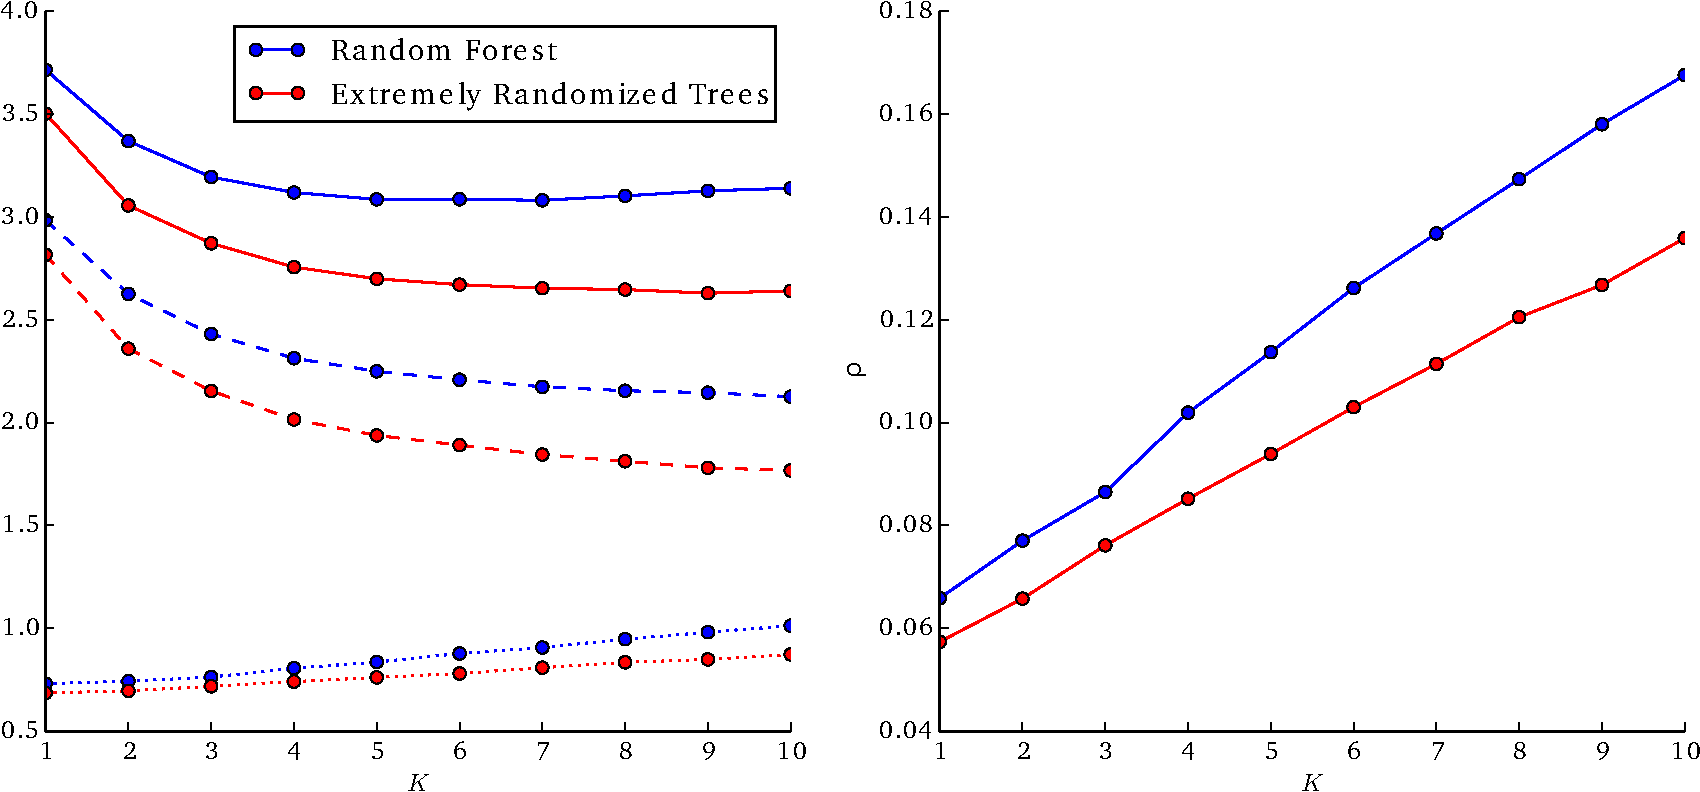
\includegraphics[width=\textwidth]{figures/ch4_correlation.pdf}
    \caption{(Left) Bias-variance decomposition of the generalization error
            with respect to the hyper-parameter $K$. The total error is shown by the plain
            lines. Bias and variance terms are respectively shown by the dashed and dotted
            lines.  (Right) Average correlation
            coefficient $\rho(\mathbf{x})$ over the predictions of two randomized trees
            grown from the same learning set but with different random seeds.}
    \label{fig:correlation}
\end{figure}
\begin{figure}
    \centering
    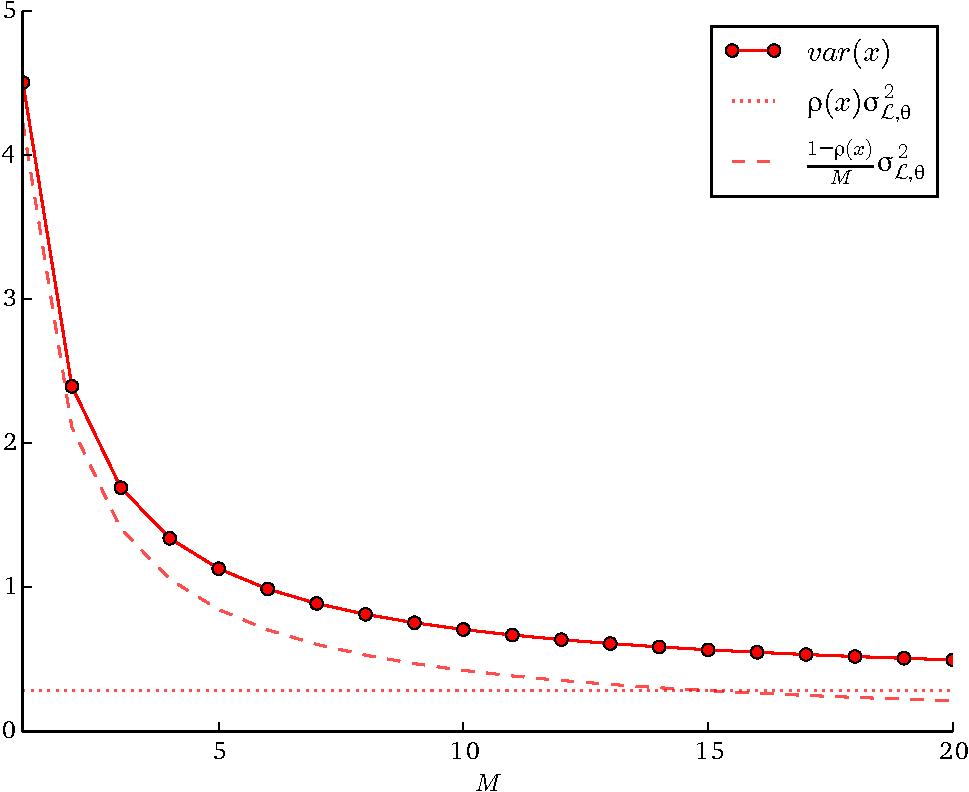
\includegraphics[width=0.9\textwidth]{figures/ch4_variance.pdf}
    \caption{Decomposition of the variance term $\text{var}(\mathbf{x})$ with respect to the number $M$ of trees in the ensemble.}
    \label{fig:variance}
\end{figure}

As the left plot in Figure~\ref{fig:correlation} shows,  the expected
generalization error additively decomposes into (squared) bias and variance
terms.  For small values of $K$, random effects are strong, leading to high
bias and low variance. By contrast, for larger values of $K$, random effects
are less important, reducing bias but increasing variance.   For both methods,
too small a value of $K$ appears however to lead to a too large increase of
bias, for which averaging is not able to compensate. For RF, the optimal
trade-off is at $K=8$, which indicates that bagging and random variable selection are
here complementary with regard to the level of randomness injected into the
trees. Indeed, using bagging only (at $K=10$) for randomizing the construction
of the trees yield results that are slighlty worse than when both techniques
are combined. For ETs, the optimal trade-off is at $K=10$, suggesting that
random thresholds $v$ provide by themselves enough randomization on this
problem.

The right plot of Figure~\ref{fig:correlation} illustrates the (averaged)
correlation coefficient $\rho(\mathbf{x})$ between the predictions of two
randomized trees grown on the same learning set. As expected, the smaller $K$,
the stronger the random effects, therefore the less correlated the predictions
and the more variance can be reduced from averaging. The plot also confirms
that ETs are inherently less correlated than trees built
in RF, which is not surprising given the fact that the former
method randomizes the choice of the discretization threshold while the latter
does not. In cases where such a randomization does not induce too large an
increase of bias, as in this problem, ETs are therefore
expected to yield better results than RF.  (The choice of the
optimal randomization strategy is however highly dependent on the problem and
no general conclusion should be drawn from this toy regression problem.)

As confirmed by Figure~\ref{fig:variance} for RF, variance also additively decomposes  into
\begin{equation}
\text{var}(\mathbf{x}) = \rho(\mathbf{x}) \sigma^2_{{\cal L},\theta}(\mathbf{x}) + \tfrac{1 - \rho(\mathbf{x})}{M} \sigma^2_{{\cal L},\theta}(\mathbf{x}).
\end{equation}
The first term is the variance due to the learning set ${\cal L}$ and remains
constant as the number $M$ of trees increases. The second term is the variance
due to random effects and decreases as $M$ increases. Of particular interest is
variance at $M=1$, which corresponds to the variance of a single decision tree.
As the figure clearly shows, averaging several decision trees into an ensemble
allows to significantly reduce this quantity. At the limit, when $M\to \infty$,
variance tends to $\rho(\mathbf{x}) \sigma^2_{{\cal L},\theta}(\mathbf{x})$, as shown by
the dotted line and as expected from Theorem~\ref{thm:bias-variance:ensemble}.

\section{Properties and features}
\label{sec:4:features}

\subsection{Out-of-bag estimates}

An interesting  feature of ensemble methods that construct models
on bootstrap samples, like Bagging or Random Forests, is the built-in possibility of
using the left-out samples ${\cal L}\setminus {\cal L}^m$ to form
estimates of important statistics. In the case of generalization error, the
\textit{out-of-bag} estimate at $(\mathbf{x}_i,y_i)$ consists in evaluating the
prediction of the ensemble using only the individual models $\varphi_{{\cal
L}^m}$ whose bootstrap samples ${\cal L}^m$ did not include
$(\mathbf{x}_i,y_i)$. That is, in regression,
\begin{align}\label{eqn:oob-error}
\widehat{Err}^\text{OOB}(\psi_{\cal L}) &= \frac{1}{N} \sum_{(\mathbf{x}_i,y_i) \in {\cal L}} L(\frac{1}{M^{-i}} \sum_{l=1}^{M^{-i}} \varphi_{{\cal L}^{m_{k_l}}}(\mathbf{x}_i), y_i),
\end{align}
where $m_{k_1}, \dots, m_{k_{M^{-i}}}$ denote the indices of $M^{-i}$ the trees that
have been built from bootstrap replicates that do not include $(\mathbf{x}_i,
y_i)$. For classification, the out-of-bag estimate of the generalization error is similar to
Equation~\ref{eqn:oob-error}, except that the out-of-bag average prediction is
replaced with the class which is the most likely, as computed from the out-of-bag
class probability estimates.

Out-of-bag estimates provide accurate estimates of the
generalization error of the ensemble, often yielding statistics that are as
good or even more precise than $K$-fold cross-validation
estimates~\citep{wolpert:1999}. In practice, out-of-bag estimates also
constitute a computationally efficient alternative to $K$-fold cross-validation,
reducing to $M$ the number of invocations of the learning
algorithm, instead of otherwise having to build $K\times M$ base models.

While out-of-bag estimates constitute an helpful tool, their benefits should
however be put in balance with the potential decrease of accuracy that the use
of bootstrap replicates may induce. As shown experimentally in
\citep{louppe:2012}, bootstrapping is in fact rarely crucial for random forests
to obtain good accuracy. On the contrary, not using bootstrap samples usually
yield better results.

\subsection{Variable importances}

In most machine learning tasks, the goal is not only to find the most accurate
model of the response but also to identify which of the input variables are the
most important to make the predictions, e.g., in order to lead to a deeper
understanding of the problem under study.

In this context, random forests offer several mechanisms for assessing the
\textit{importance} of an input variable, and therefore enhance the
interpretability of the model. These are the object of
Chapter~\ref{ch:importances}, in which we study variable importance measures
and develop original contributions to further improve their understanding.

\subsection{Proximity measures}

Another helpful built-in feature of tree-based ensemble methods is the
\textit{proximity measure}~\citep{breiman:2002} between two sample points. Formally, the proximity
between $(\mathbf{x}_1, y_1)$ and $(\mathbf{x}_2, y_2)$ is defined as the
number of times both samples reach the same leaf $t$ within each decision tree,
normalized by the number of trees in the forest. That is,
\begin{equation}
\text{proximity}(\mathbf{x}_1, \mathbf{x}_2) = \frac{1}{M} \sum_{m=1}^M \sum_{t \in \widetilde{\varphi}_{{\cal L},\theta_m}} 1(\mathbf{x}_1 , \mathbf{x}_2 \in {\cal X}_t)
\end{equation}
where $\widetilde{\varphi}_{{\cal L},\theta_m}$ denotes the set of terminal
nodes in $\varphi_{{\cal L},\theta_m}$. The idea is that the proximity measure
gives an indication of how close the  samples are in the eyes of the random
forest~\citep{hastie:2005}, even if the data is high-dimensional or involves
mixed input variables. When proximity is close to $1$, samples propagate into
the same leaves and are therefore similar according to the forest. On the other
hand, when it is close to $0$, samples reach different leaves, suggesting that
they are structurally different from each other. The proximity measure
depends on both the depth and the number of trees in the forest.
When trees are shallow, samples are more likely to end up in the same leaves
than when trees are grown more deeply, thereby impacting on the spread of the measure.
Likewise, the more trees in the forest, the smoother the measure since
the larger the number $M+1$ of values the proximity measure can take.

\begin{figure}
    \centering
    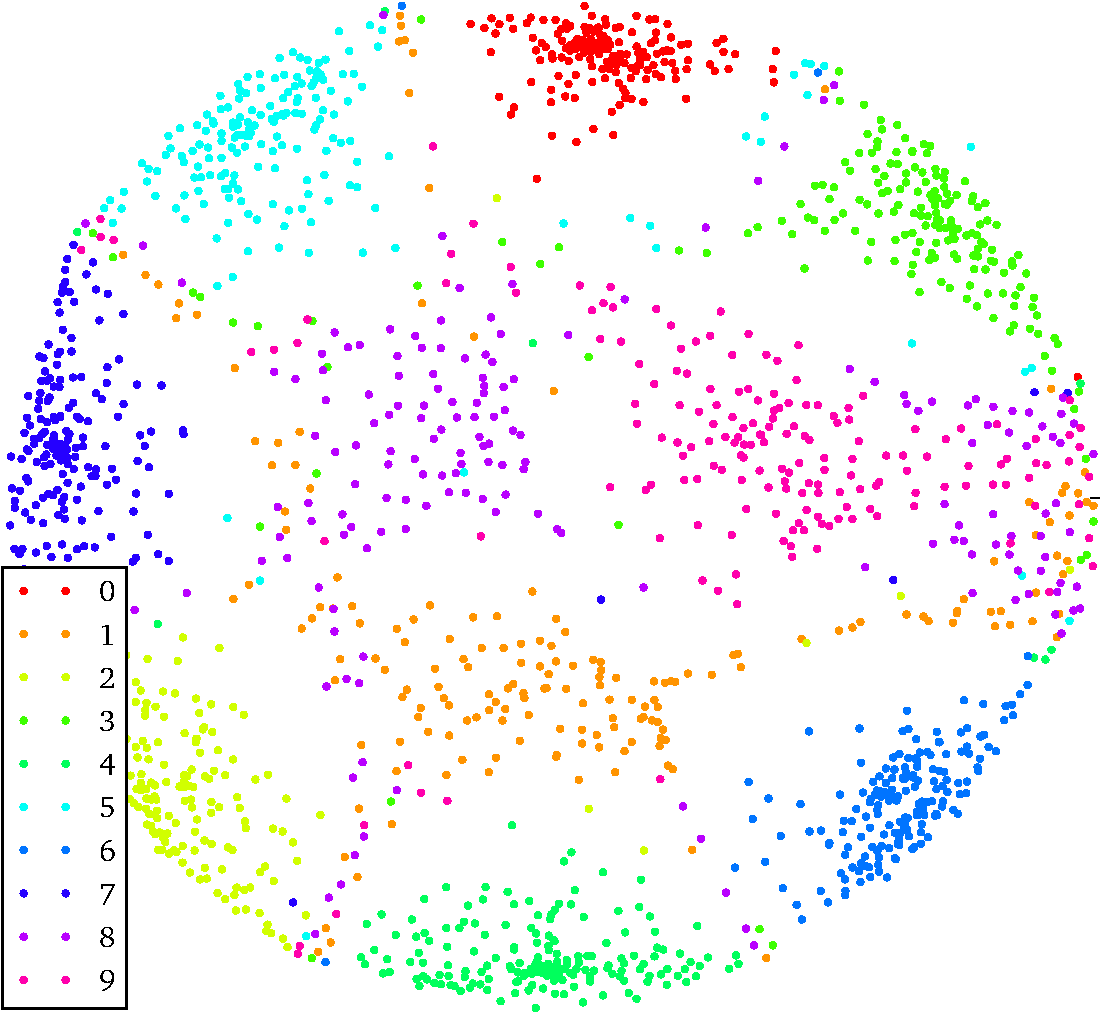
\includegraphics[width=0.9\textwidth]{figures/ch4_proximity_plot.pdf}
    \caption{Proximity plot for a 10-class handwritten digit classification task.}
    \label{fig:proximity-plot}
\end{figure}

For exploratory purposes, the $N\times N$ proximity matrix $P$ such that
\begin{equation}
P_{ij} = \text{proximity}(\mathbf{x}_i, \mathbf{x}_j),
\end{equation}
can be used to visually represent how samples are close together with respect
to the random forest. Using $1-P$ as a dissimilarity matrix,  the level of
similarity between individual samples can be visualized e.g., by projecting them
on a $d$-dimensional space (e.g., on a plane) such that the distances
between any pair of samples in that space correspond as best as possible to the
dissimilarities in $1-P$. As an illustrative example, Figure~\ref{fig:proximity-plot}
represents the proximity matrix learned for a 10-class handwritten digit
classification task, as projected on a plane using Multidimensional Scaling~\citep{kruskal:1964}.
Samples from a same class form identifiable clusters, which suggests that
they share similar structure (since they end up in the same leaves). The figure
also highlights classes for which the random forest makes errors. In this case,
digits $1$ and $8$ are the more dispersed, suggesting high within-class variance,
but also overlap the most with samples of other classes, indicating
that the random forest fails to identify the true class for these samples.

Additionally, proximity measures can be used for identifying outliers within a
learning set ${\cal L}$. A sample $\mathbf{x}$ can be considered as an outlier
if its average proximity with respect to all other samples is small, which
indeed indicates that $\mathbf{x}$ is structurally different from the other
samples (since they do not end up in the same leaves). In the same way, in
classification, within-class outliers can be identified by computing the
average proximity of a sample with respect to all other samples of the same
class. Conversely, proximity measures can be used for identifying class
prototypes, by considering samples whose proximity with all other samples
of the same class is the largest.

An alternative formulation of proximity measures is to consider a random forest
as a mapping $\phi: {\cal X} \mapsto {\cal X}^\prime$ which transforms a sample
$\mathbf{x}$ into the (one-hot-encoded) indices of the leaves it ends up in.
That is, $\mathbf{x}^\prime_t$ is $1$ for all leaves $t$ of the forest in which
$\mathbf{x}$ falls in, and $0$ for all the others:
\begin{equation}
\phi(\mathbf{x}) = \Big( 1(\mathbf{x} \in {\cal X}_{t_1}), \dots, 1(\mathbf{x} \in {\cal X}_{t_L} ) \Big)
\end{equation}
where $t_1, \dots, t_L \in \widetilde{\psi}$ denote the leafs of all $M$ trees in the forest $\psi$.
In this formalism, the
proximity between $\mathbf{x}_1$ and $\mathbf{x}_2$ corresponds to a
\textit{kernel}~\citep{scholkopf:2001}\label{ntn:kernel2}, that can be defined as the normalized
dot product of the samples, as represented in ${\cal X}^\prime$:
\begin{equation}
\text{proximity}(\mathbf{x}_1, \mathbf{x}_2) = \frac{1}{M} \phi(\mathbf{x}_1) \cdot \phi(\mathbf{x}_2)
\end{equation}
Interestingly, $\phi$ provides a non-linear transformation to a sparse very
high-dimensional space, taking somehow into account the structure of the
problem. If two samples are structurally similar, then they will end up in the
same leafs and their representations in the projected space will be close, even
if they may in fact appear quite dissimilar in the original space.

In close connection, \citep{geurts:2006} show that a regression tree
$\varphi$ can be expressed as a kernel-based model by formulating the
prediction $\varphi(\mathbf{x})$ as a scalar product over the input space
defined by the normalized characteristic function $\phi^\prime$ of the leaf nodes. That is,
\begin{equation}
\varphi(\mathbf{x}) = \sum_{(\mathbf{x}_i, y_i) \in {\cal L}} y_i K_\varphi(\mathbf{x}_i, \mathbf{x})
\end{equation}
where
\begin{align}
K_\varphi(\mathbf{x}_i, \mathbf{x}) &= \phi^\prime(\mathbf{x}_i) \cdot \phi^\prime(\mathbf{x}), \\
\phi^\prime(\mathbf{x}) &= \Big( \frac{1(\mathbf{x} \in {\cal X}_1)}{\sqrt{N_1}}, \dots, \frac{1(\mathbf{x} \in {\cal X}_{t_L})}{\sqrt{N_{t_L}}}  \Big),
\end{align}
and where $t_1,\dots,t_L \in \widetilde{\varphi}$ denote the leafs of $\varphi$.
Likewise, the formulation can be extended to an ensemble $\psi$ of $M$ decision
trees by defining $K_\psi$ as the average kernel over $K_{\varphi_m}$ (for $m=1,\dots,M$).

From a more practical point of view, such forest-based transforms $\phi$ and
$\phi^\prime$ have proven to be helpful and efficient embeddings, e.g., when
combined with linear methods or support vector machines
\citep{moosmann:2006,maree:2013}. In particular, they find useful applications
in computer vision for transforming the raw pixel input space into a new
feature space hopefully capturing structures and patterns in images.

\subsection{Missing data}

Because of practical limitations, physical constraints or for privacy reasons,
real-world data are often imperfect, erroneous or incomplete. In particular,
most machine learning algorithms are often not applicable on data containing
missing values because they implicitely assume an ideal scenario in which all
values are known for all input variables. Fortunately, random forests offer
several mechanisms for dealing with this issue.

\begin{description}

\item \textit{Ternary decision trees.}\hfill\\
    The simplest strategy is to explicitely model missing values in the
    structure of decision trees by considering ternary splits instead of binary
    splits. That is, partition $t$ into $t_L$, $t_R$ and $t_M$, such that $t_L$
    and $t_R$ are defined from a binary split $s_j^v : X_j \leq v$, for all node
    samples where the value of $X_j$ is known, and such that $t_M$ contain all node
    samples for which the value of $X_j$ is missing.

\item \textit{Propagate in both child nodes}\hfill\\
    An alternative strategy is to  propagate samples
    for which the value of the split variable is missing into both the left and
    right child nodes. Accordingly, samples going into both child nodes should be
    reweighted by half their sample weight (see Chapter~\ref{ch:complexity}), so
    that they are not unfairly taken into account more than the other samples.

\item \textit{Imputation.}\hfill\\
    Finally, random forests also offer several mechanisms for imputing missing
    values. A simple approach, due to \citep{breiman:2002}, consists first in
    filling missing values with a rough and inaccurate approximation (e.g., the
    median). Then build a random forest on the completed data and update the
    missing values of each sample by the weighted mean value over the samples
    that are the closest (as defined by the proximity measure). The procedure
    is then repeated  until convergence, typically after $4$ to $6$ iterations.

    Alternatively, missing data imputation can be considered as a supervised
    learning problem in itself, where the response variable is the input
    variable for which values are missing. As such, the MissForest
    algorithm~\citep{stekhoven:2012} consists in iteratively building a random
    forest on the observed parts of the data in order to predict the missing
    values for a given variable.

\end{description}


\section{Consistency}
\label{sec:4:consistency}

Despite their extensive use in practice, excellent performance and relative
algorithmic simplicity, the mathematical mechanisms that drive random forests
are still not well understood. More specifically, the fundamental theoretical
question of the consistency (see definitions~\ref{def:consistency} and
\ref{def:consistency-strong}) of random forests, i.e., whether convergence towards an
optimal model is guaranteed provided an infinitely large learning set, remains
an open and difficult problem. In this section, we review theoretical works
that have investigated simplified versions of the algorithm, for which the
theoretical analysis is typically more tractable. With the hope that results
obtained for these simplified models will provide insights on the mathematical
properties of the actual algorithm, the long-term objective of this line of
research is usually to prove the consistency of the original Random Forest
algorithm \citep{breiman:2001}, hence bridging the gap between theory and
practice.


\begin{description}

\item \citet{breiman:1984}:\hfill \\
    Single decision trees are proved to be consistent, both in regression and
    classification.

    Note that these results do not extend to the Random Forest algorithm for the following reasons:
    \begin{itemize}
    \item In single decision trees, the number of samples in terminal nodes
          is let to become large, while trees in random forests are usually fully developed;
    \item Single decision trees do not make use of bootstrap sampling;
    \item The splitting strategy in single decision trees consists in selecting
          the split that maximizes the Gini criterion. By contrast, in random forests,
          the splitting strategy is randomized.
    \end{itemize}

\item \citet{zhao:2000}:\hfill\\
    One of the earliest works studying the consistency of ensembles of
    randomized trees is due to \citet{zhao:2000}. In classification, the author
    conjectures that PERT is (weakly) consistent, but establishes its strong
    consistency (Theorem 4.4.2) provided the construction of the trees stops early. More
    specifically, strong consistency is guaranteed provided:

    \begin{enumerate}
        \item Trees are grown
            infinitely deeply while forming leaves with infinitely many node samples,
            hence making empirical class proportions in terminal nodes
            converge towards their theoretical counterparts. This is guaranteed,
            e.g.,  by stopping the construction
            when $N_t < N_\text{min}$, such that
            $N_\text{min} \to 0$ and  $N\times N_\text{min} \to \infty$ as $N \to
            \infty$;

        \item The posterior class probabilities induced by the ensemble are all
              continuous in the input space ${\cal X}$.
    \end{enumerate}

    Given the close formulations of the methods, results from \citep{zhao:2000}
    regarding PERT extend to Extremely Randomized Trees provided the posterior
    class probabilities are continuous. In Appendix F of \citep{geurts:2006},
    Extremely Randomizes Trees (for $K=1$ and $M \to \infty$) are shown
    to be a continuous piecewise multilinear function of its arguments,
    which suffices to establish the strong consistency of the method when
    trees are built totally at random.

\item \citet{breiman:2004}:\hfill\\
    In this work, consistency is studied for a simplified variant of the Random
    Forest algorithm, assuming (i) no bootstrap sampling, (ii) that splits on
    relevant variables are set at the midpoint of the values of the selected
    variable, (iii) that splits on irrelevant variables are set at random points
    along the values of the selected variable and (iv) that trees are balanced.
    Under these assumptions,  it can be shown that this variant reduces
    to a nearest neighbor algorithm~\citep{lin:2006}, for which consistency
    conditions are met.

\item \citet{biau:2008}:\hfill\\

\item \citet{biau:2012}:\hfill \\

\item \citet{denil:2013}:\hfill \\

\item \citet{scornet:2014}:\hfill \\

\end{description}


% Zhao
% Biau 2008, 1 feature, split au hasard dans un gap aléatoire, open node tirée au hasard. Stop after M_L leafs
% Genuer 2010 Risk bounds for purely uniformly random forests.
% Genuer 2012 Variance reduction in purely random forests.
% Biau 2012, K features, threshold = mid-point dans le range du noeud, bread-first jusqu'à M_L leafs. Dataset != for splitting than for assigning
% Denil 2012 Narrowing the gap: Random forests in theory and in practice.
% Scornet 2014 http://arxiv.org/abs/1405.2881

% Conclusion: extend to a larger class of  tree algorithms
% strong?
% universal?


    % > Mise au point
    % > Preuve de consistence des extra-trees?
    % Devroye et al., 1996, Chapter 20
    % Thèse de david matheson

\chapter{Computational efficiency}\label{ch:complexity}

\begin{remark}{Outline}
In this chapter, we study the computational efficiency of tree-based ensemble
methods. In sections~\ref{sec:5:complexity-fit} and \ref{sec:5:complexity-predict},
we derive and discuss the time complexity of random forests, first for building them from data and then for making predictions. In
Section~\ref{sec:5:impl}, we discuss technical details that are critical
for efficiently  implementing random forests. Finally, we conclude in
Section~\ref{sec:5:benchmarks} with benchmarks of the random forest implementation developed
within this work and compare our solution with alternative implementations.
\end{remark}

\section{Complexity of the induction procedure}
\label{sec:5:complexity-fit}

The dominant objective of most machine learning methods is to find models that
maximize accuracy. For models of equivalent performance, a secondary objective
is usually to minimize complexity. Complexity, however, has many facets. A
first and immediate notion of complexity in decision trees and random forests is
the \textit{time complexity} for learning models, that is the number of
operations required for building models from data.

Given the exponential growth in the number of possible partitions of $N$
samples, we chose in Section~\ref{sec:3:splitting-rules} to restrict splitting
rules to binary splits defined on single variables. Not only this is sufficient
for reaching good accuracy (as discussed in Section~\ref{sec:4:consistency}),
it also allows for time complexity to effectively remain within reasonable bounds.

Formally, let $T(N)$ denotes the time complexity for building a decision tree from a
learning set ${\cal L}$ of $N$ samples. From Algorithm~\ref{algo:induction},
$T(N)$ corresponds to the number of operations required for splitting a node of $N$ samples and then for recursively
building two sub-trees respectively from $N_{t_L}$ and $N_{t_R}$ samples. Without
loss of generality, let us assume that the learning samples all have distinct
input values, such that it is possible to build a fully developed decision tree
where each leaf contains exactly one sample. Under this assumption, determining
time complexity therefore amounts to solve the recurrence equation
\begin{equation}\label{eqn:complexity:rec}
\begin{cases}
T(1) = O(1) \\
T(N) = c(N) + T(N_{t_L}) + T(N_{t_R}),
\end{cases}
\end{equation}
where $c(N)$ is the time complexity for splitting a node of $N$ samples. For
$N=1$, the node is necessarily pure, hence the constant time complexity $O(1)$.
For $N>1$, $c(N)$ corresponds to the time complexity for finding a split $s$
and then partitioning the node samples into ${t_L}$ and ${t_R}$. This later
operation requires at least to iterate over all $N$ samples, which sets a
linear lower bound on time complexity within a node, i.e., $c(N)=\Omega(N)$. As
for finding the split $s$, this can be achieved in several ways, as outlined in
the previous chapters  for several randomized variants of the induction
procedure. As we will see, not only this is an impact on the accuracy of the
resulting model, it also drives the time complexity of the induction procedure.

\begin{remark}{Big O notations}
Time complexity analyzes the asymptotic behavior of an algorithm
with respect to the size $N$ of its input and its hyper-parameters. In this way,
big O notations are used to formally express an asymptotic upper bound on the
growth rate of the number $f(N)$ of steps in the algorithm. Formally,
we write that
\begin{equation}
f(N) =  O(g(N)) \ \text{if}\ \exists c > 0, N_0 > 0, \forall N > N_0, f(N) \leq c g(N)
\end{equation}
to express that  $f(N)$ is asymptotically upper bounded by $g(N)$, up to some neglectable constant factor $c$.
Similarly, big $\Omega$ notations are used to express an asymptotic lower
bound on the growth rate of the number of steps in the algorithm. Formally,
we write that
\begin{equation}
f(N) =  \Omega(g(N)) \ \text{if}\ \exists c > 0, N_0 > 0, \forall N > N_0,  c g(N) \leq f(N)
\end{equation}
to express that $f(N)$ is asymptotically lower bounded by $g(N)$.
Consequently, if $f(N)$ is both $O(g(N))$ and $\Omega(g(N))$ then $f(N)$ is
both lower bounded and upper bounded asymptotically by $g(N)$ (possibly for different constants),
which we write using big $\Theta$ notations:
\begin{equation}
f(N) = \Theta(g(N)) \ \text{if}\  f(N) =  O(g(N)) = \Omega(g(N)).
\end{equation}
\end{remark}

In the original CART induction procedure~\citep{breiman:1984}
(Algorithms~\ref{algo:findsplit} and \ref{algo:findsplit:x_j}), finding a split
$s$  requires, for each of the $p$ variables $X_j$ (for $j=1,\dots,p$), to sort
the values $x_{i,j}$ of all $N$ node samples (for $i=1,\dots,N$) and then to
iterate over these in order to find the best threshold $v$. The most costly
operation is sorting, whose time complexity is at worst $O(N \log N)$. As a
result, the overall within-node complexity is $c(N) = O(p N \log N)$. In a
randomized tree as built with the Random Forest algorithm~\citep{breiman:2001}
(RF, Algorithm~\ref{algo:findsplit:random}), the search of the best split $s$
is carried out in the same way, but only on $K \leq p$ of the input variables,
resulting in a within-node complexity $c(N) = O(K N \log N)$. In Extremely
Randomized Trees~\citep{geurts:2006} (ETs, Algorithm~\ref{algo:findsplit:et}),
discretization thresholds are drawn at random within the minimum and maximum
node sample values of $X_j$, making sort no longer necessary. As such, the
within-node complexity reduces to the time required for finding these lower and
upper bounds, which can be done in linear time, hence $c(N)=O(KN)$. Finally, in
Perfect Random Tree Ensembles~\citep{cutler:2001} (PERT,
Algorithm~\ref{algo:findsplit:pert}), cut-points $v$ are set midway between
two randomly drawn samples, which can be done in constant time, independently
of the number $N$ of node samples. Yet, the within-node complexity is lower
bounded by the time required for partitioning the node samples into ${t_L}$ and
${t_R}$, hence $c(N)=O(N)$.

Since both CART and PERT can respectively be considered as special cases of RF
and ETs with regards to time complexity (i.e., for $K=p$ in CART, for $K=1$ in
PERT), let us consider the overall complexity $T(n)$ when either
$c(N)=O(KN\log N)$ or $c(N)=O(KN)$ (for $K=1,\dots,p$). Time complexity
is studied in three cases:

\begin{itemize}
\item \textit{Best case.} The induction procedure is the most effective
      when node samples can always be partitioned into two balanced subsets of $\tfrac{N}{2}$
      samples.

\item \textit{Worst case.} By contrast, the induction procedure is the least
      effective when splits are unbalanced. In the worst case,
      this results in splits that move a single sample in the first sub-tree and
      all $N-1$ others in the second sub-tree.

\item \textit{Average case.} The average case corresponds to the average time
      complexity, as taken over all possible learning sets ${\cal L}$ and
      all random seeds $\theta$.  Since the analysis of this case is hardly
      feasible without strong assumptions on the structure of the problem,
      we consider instead the case where the sizes of the possible
      partitions of a node are all equiprobable.

\end{itemize}

\begin{remark}{Master Theorem}
Some of the results outlined in the remaining of this section make use of the
Master Theorem~\citep{goodrich:2006}, which recall below to be self-contained.

\begin{theorem}
Let consider the recurrence equation
\begin{equation}
\begin{cases}
T(1) = c & \text{if}\quad n < d\\
T(n) = aT(\frac{n}{b}) + f(n) & \text{if}\quad n \geq d
\end{cases}
\end{equation}
where $d \geq 1$ is an integer constant, $a > 0$, $c>0$ and $b>1$ are real constants, and
$f(n)$ is a function that is positive for $n \geq d$.

\begin{enumerate}
\item If there is a small constant $\epsilon > 0$, such that $f(n)$ is $O(n^{\log_b a - \epsilon})$, then $T(n)$ is $\Theta(n^{\log_b a})$.
\item If there is a constant $k \geq 0$, such that $f(n)$ is $O(n^{\log_b a} \log^k n)$, then $T(n)$ is $\Theta(n^{\log_b a} \log^{k+1} n)$.
\item If there are small constants $\epsilon > 0$ and $\delta < 1$, such that $f(n)$ is $\Omega(n^{\log_b a + \epsilon})$ and $af(\tfrac{n}{b}) \leq \delta f(n)$, for $n \geq d$, then $T(n)$ is $\Theta(f(n))$.
\end{enumerate}
\end{theorem}
\end{remark}

\begin{theorem}\label{thm:6:best:knlogn}
For $c(N)=O(K N\log N)$, the time complexity for building a decision
tree in the best case is $O(K N \log^2 N)$.
\end{theorem}

\begin{proof}
Since $O(K)=O(1)$, the dependency to $K$ in Equation~\ref{eqn:complexity:rec} can be factored out,
thereby rewriting $T(N)$ as $O(K) T'(N)$, where $T'(N)$ is
\begin{equation}
\begin{cases}
T'(1) = O(1) \\
T'(N) = O(N\log N) + 2 T'(\frac{N}{2})
\end{cases}
\end{equation}
in the best case. In this form, the second case of the Master Theorem applies for
$a=2$, $b=2$ and $k=1$. Accordingly, $T'(N)=O(N\log^{k+1} N)=O(N\log^2 N)$ and $T(N) = O(K N\log^2 N)$.
\end{proof}

\begin{theorem}\label{thm:6:best:kn}
For $c(N)=O(K N)$, the time complexity for building a decision
tree in the best case is $O(K N \log N)$.
\end{theorem}

\begin{proof}
For $T(N) = O(K)T'(N)$, Equation~\ref{eqn:complexity:rec}
can be rewritten in the best case as
\begin{equation}
\begin{cases}
T'(1) = O(1) \\
T'(N) = O(N) + 2 T'(\frac{N}{2})
\end{cases}
\end{equation}
Again, the second case of the Master Theorem applies, this time for $a=2$, $b=2$ and $k=0$.
Accordingly, $T'(N)=O(N\log^{k+1} N)=O(N\log N)$ and $T(N) = O(K N\log N)$.
\end{proof}

\begin{theorem}\label{thm:6:worst:knlogn}
For $c(N)=O(K N\log N)$, the time complexity for building a decision
tree in the worst case is $O(K N^2 \log N)$.
\end{theorem}

\begin{proof}
For $T(N) = O(K)T'(N)$, Equation~\ref{eqn:complexity:rec}
can be rewritten in the worst case as
\begin{equation}
\begin{cases}
T'(1) = O(1) \\
T'(N) = O(N\log N) +  T'(1) + T'(N-1).
\end{cases}
\end{equation}
By expanding the recurrence, we have
\begin{align}
T'(N) &= O(N\log N) + O(1) + T'(N-1) \nonumber \\
      &= \sum_{i=1}^N O(1) + O(i\log i) \nonumber \\
      &= O(N) + \sum_{i=1}^N O(i\log i) \nonumber \\
      &\leq O(N) + O(\log N) \sum_{i=1}^N O(i) \nonumber \\
      &= O(N) + O(\log N) O(\frac{1}{2} N(N+1) \nonumber \\
      &= O(N^2 \log N).
\end{align}
As a result, $T(N) = O(K N^2 \log N)$ in the worst case.
\end{proof}

\begin{theorem}\label{thm:6:worst:kn}
For $c(N)=O(K N)$, the time complexity for building a decision
tree in the worst case is $O(K N^2)$.
\end{theorem}

\begin{proof}
For $T(N) = O(K)T'(N)$, Equation~\ref{eqn:complexity:rec}
can be rewritten in the worst case as
\begin{equation}
\begin{cases}
T'(1) = O(1) \\
T'(N) = O(N) +  T'(1) + T'(N-1)
\end{cases}
\end{equation}
By expanding the recurrence, we have
\begin{align}
T'(N) &= O(N) + O(1) + T'(N-1) \nonumber \\
      &= O(1) + \sum_{i=2}^N O(1+i) \nonumber \\
      &= O(1) + O(\frac{1}{2} (N^2 + 3N - 4)) \nonumber \\
      &= O(N^2).
\end{align}
As a result, $T(N) = O(K N^2)$ in the worst case.
\end{proof}

\begin{theorem}\label{thm:6:average:knlogn}
For $c(N)=O(K N\log N)$, the time complexity for building a decision
tree in the average case is $O(K N \log^2 N)$.
\end{theorem}

\begin{proof}
For $T(N) = O(K)T'(N)$, Equation~\ref{eqn:complexity:rec}
can be rewritten in the average case as
\begin{equation}
\begin{cases}
T'(1) = O(1) \\
T'(N) = O(N\log N) +  \frac{1}{N-1} \sum_{i=1}^{N-1} T'(i) + T'(N-i).
\end{cases}
\end{equation}
By symmetry and by multiplying both sides of the last equation by $(N-1)$, it comes
\begin{equation}\label{eqn:6:average:knlogn:1}
(N-1) T'(N) = O(N\log N)(N-1) +  2 \sum_{i=1}^{N-1} T'(i).
\end{equation}
For $N \geq 3$, substituting $N$ with $N-1$ similarly yields
\begin{equation}\label{eqn:6:average:knlogn:2}
(N-2) T'(N-1) = O((N-1) \log(N-1))(N-2) +  2 \sum_{i=1}^{N-2} T'(i).
\end{equation}
Subtracting Equation~\ref{eqn:6:average:knlogn:2} from \ref{eqn:6:average:knlogn:1},
it comes after simplifications and division of both sides by $N(N-1)$:
\begin{equation}
\frac{T'(N)}{N} = \frac{T'(N-1)}{N-1} + O(\frac{2}{N} \log(N-1) + \log \frac{N}{N-1} ).
\end{equation}
Let us now introduce $S(N) = \frac{T'(N)}{N}$. From the last equation, it comes
\begin{align}
S(N) &= S(N-1) + O(\frac{2}{N} \log(N-1) + \log \frac{N}{N-1} ) \nonumber \\
     &= O(1) + O(\sum_{i=2}^N \frac{2}{i} \log(i-1) + \log \frac{i}{i-1} ) \nonumber \\
     &= O(1) + O(\log N) + O(2 \sum_{i=2}^N \frac{1}{i} \log(i-1) ) \nonumber \\
     &\leq O(1) + O(\log N) + O(2 \log N) O(\sum_{i=2}^N \frac{1}{i} ) \nonumber \\
     &= O(1) + O(\log N) + O(2 \log N) O(H_N - 1) \nonumber \\
     &= O(H_N \log N)
\end{align}
where $H_N$ is the $N$-th harmonic number. Using
\begin{equation}
H_N \approx \log N + \gamma + \frac{1}{2N} + O(\frac{1}{N^2})
\end{equation}
as approximation (where $\gamma$ is the Euler-Mascheroni constant), we have
\begin{align*}
T'(N) &= O(N H_N \log N) \nonumber \\
      &= O(N (\log N + \gamma + \frac{1}{2N} + \frac{1}{N^2}) \log N  ) \nonumber \\
    &= O(N \log^2 N).
\end{align*}
As a result, $T(N) = O(KN \log^2 N)$ in the average case.
\end{proof}

\begin{theorem}\label{thm:6:average:kn}
For $c(N)=O(K N)$, the time complexity for building a decision
tree in the average case is $O(K N \log N)$.
\end{theorem}

\begin{proof}
For $T(N) = O(K)T'(N)$, Equation~\ref{eqn:complexity:rec}
can be rewritten in the average case as
\begin{equation}
\begin{cases}
T'(1) = O(1) \\
T'(N) = O(N) +  \frac{1}{N-1} \sum_{i=1}^{N-1} T'(i) + T'(N-i).
\end{cases}
\end{equation}
By symmetry and by multiplying both sides of the last equation by $(N-1)$, it comes
\begin{equation}\label{eqn:6:average:kn:1}
(N-1) T'(N) = O(N)(N-1) +  2 \sum_{i=1}^{N-1} T'(i).
\end{equation}
For $N \geq 3$, substituting $N$ with $N-1$ similarly yields
\begin{equation}\label{eqn:6:average:kn:2}
(N-2) T'(N-1) = O(N-1)(N-2) +  2 \sum_{i=1}^{N-2} T'(i).
\end{equation}
Subtracting Equation~\ref{eqn:6:average:kn:2} from \ref{eqn:6:average:kn:1},
it comes after simplifications and division of both sides by $N(N-1)$:
\begin{equation}
\frac{T'(N)}{N} = \frac{T'(N-1)}{N-1} + O(\frac{2}{N}).
\end{equation}
Let us now introduce $S(N) = \frac{T'(N)}{N}$. From the last equation, it comes
\begin{align}
S(N) &= S(N-1) + O(\frac{2}{N}) \nonumber \\
     &= O(2 \sum_{i=1}^N \frac{1}{i} ) \nonumber \\
     &= O(2 H_N)
\end{align}
where $H_N$ is the $N$-th harmonic number. Using
\begin{equation}
H_N \approx \log N + \gamma + \frac{1}{2N} + O(\frac{1}{N^2})
\end{equation}
as approximation (where $\gamma$ is the Euler-Mascheroni constant), we have
\begin{align}
T'(N) &= O(2 H_N N) \nonumber \\
&= O(2 N \log N + 2 N\gamma + 1 + \frac{2}{N}) \nonumber \\
&= O(N \log N).
\end{align}
As a result, $T(N) = O(KN \log N)$ in the average case.
\end{proof}

From Theorems~\ref{thm:6:best:knlogn}-\ref{thm:6:average:kn}, the total time
complexity for building an ensemble of $M$ randomized trees can finally be
derived. As summarized in Table~\ref{table:complexity-fit}, complexity remains
within reasonable bounds for all variants studied in this work. In the best
case, complexity is linear with the number of split variables considered at
each node (i.e., $O(K)$) and linearithmic or quasilinear with the number of
(unique) samples effectively used to build each tree (i.e., $O(N\log N)$ or
$O(N\log^2 N)$). In the very worst case however, this later dependency becomes quadratic
(i.e., $O(N^2)$ or $O(N^2 \log N)$, which might greatly affect performance in
the context of large datasets. Reassuringly, the analysis of the average case
shows that pathological cases are not dominant and that, on average, complexity
behaves as in the best case.

\begin{table}
    \centering
    \begin{tabular}{| c | c c c |}
    \hline
         & \textit{Best case} & \textit{Worst case} & \textit{Average case}  \\
    \hline
    \hline
    CART & $O(pN\log^2 N)$ & $O(pN^2\log N)$ & $O(pN\log^2 N)$ \\
    Bagging & $O(Mp\widetilde{N}\log^2 \widetilde{N})$ & $O(Mp\widetilde{N}^2\log \widetilde{N})$ & $O(Mp\widetilde{N}\log^2 \widetilde{N})$  \\
    RF & $O(MK\widetilde{N}\log^2 \widetilde{N})$ & $O(MK\widetilde{N}^2\log \widetilde{N})$ & $O(MK\widetilde{N}\log^2 \widetilde{N})$  \\
    ETs & $O(MKN\log N)$ & $O(MKN^2)$ & $O(MKN\log N)$  \\
    PERT & $O(MN\log N)$ & $O(MN^2)$ & $O(MN\log N)$  \\
    \hline
    \end{tabular}
    \caption{Time complexity for building forests of $M$ randomized trees. $N$ denotes the number of samples in ${\cal L}$, $p$ the number of input variables and $K$ the number of variables randomly drawn at each node. $\widetilde{N} = 0.632 N$, due to the fact that bootstrap samples draw, on average, $63.2\%$ of unique samples.}
    \label{table:complexity-fit}
\end{table}

As expected, the complexity of Bagging~\citep{breiman:1996b} is about $M$ times
as large as the complexity of building a single decision tree. Yet, by taking
into account the fact that bagged decision trees are built on bootstrap
replicates ${\cal L}^m$ that contain about $63.2\%$ of unique samples,
complexity can be expressed with respect to $\widetilde{N} = 0.632 N$ instead
of $N$. From an implementation point of view, repeated occurrences of the same
input vector can indeed be accounted for using sample weights for the
evaluation of the impurity criterion, thereby  simulating a learning set of $N$
samples from $\widetilde{N}$ unique samples while reducing the effective size
of the learning set. Assuming close constant factors, building a single bagged
decision tree is therefore asymptotically
\begin{equation}
\lim_{N\to \infty} \frac{N\log^2 N}{0.632N \log^2 0.632N} = 1.582
\end{equation}
times faster than building a regular decision tree. The complexity of RF is
identical to Bagging, except that the dependency
to $p$ becomes a dependency to $K$, resulting in an average speedup of
$\tfrac{p}{K}$. In other words, not only choosing $K \leq p$ improves accuracy,
it also significantly decreases the time required for building trees in a
forest. In ETs, due to the fact that
samples are no longer required to be sorted at each node, the dependency to $N$
becomes linearithmic instead of quasilinear. With respect to RF,
speedup is asymptotically $O(\log N)$. Finally, PERT shows to be the fastest
method of all, which is due to the fact that only a single split variable
is considered at each split. For $K=1$ however, ETs and PERT have identical
time complexity.

\begin{remark}{Presorting data in Random Forests}
As shown above, sorting node samples at each split significantly impacts
the overall complexity of the induction procedure. An alternative strategy is
possible~\citep{breiman:2002} and consists in presorting the samples for all
$p$ input variables before the construction of the tree. More specifically, let
$i=1,\dots,\widetilde{N}$ denote the original indices of the unique input
samples in ${\cal L}^m$. For each input variable $X_j$ (for $j=1,\dots,p$), the
sorted indices $\sigma^j_1,\dots,\sigma^j_{\widetilde{N}}$, such that
\begin{equation} x_{\sigma^j_1,j} \leq \dots \leq
x_{\sigma^j_{\widetilde{N}},j}, \end{equation} can be computed in
$O(p\widetilde{N}\log \widetilde{N})$. Given these indices, finding the best
split at a node then simply amounts to iterate, in that order, over the
samples $\smash{\sigma^j_1,\dots,\sigma^j_{\widetilde{N}}}$ (for all $K$ of the
split variables $X_j$), which reduces complexity to
$O(K\widetilde{N})$ instead of $O(K\widetilde{N}\log \widetilde{N})$.
Partitioning the node samples into $t_L$ and $t_R$ then requires to partition
all $p$ lists of sorted indices into $2p$ sub-lists of $\widetilde{N}_{t_L}$ and
$\widetilde{N}_{t_R}$ sorted indices
$\smash{\sigma^j_1,\dots,\sigma^j_{\widetilde{N}_{t_L}}}$ and
$\smash{\sigma^j_1,\dots,\sigma^j_{\widetilde{N}_{t_R}}}$, which can be done in
$O(p\widetilde{N})$. In total, the within-node complexity is
\begin{equation}
c(\widetilde{N}) = O(K\widetilde{N} + p\widetilde{N}) = O(p\widetilde{N}).
\end{equation} Using this
alternative strategy, the time complexity of RF for the best, the worst and the
average cases is respectively $O(Mp\widetilde{N}\log \widetilde{N})$,
$O(Mp\widetilde{N}^2)$ and $O(Mp\widetilde{N}\log \widetilde{N})$, as derived
from theorems~\ref{thm:6:best:kn}, \ref{thm:6:worst:kn} and
\ref{thm:6:average:kn} for $K=p$. Neglecting constant factors, the ratio between the two
implementations is $O(\frac{p}{K\log \widetilde{N}})$, which might not necessarily
lead to faster building times depending on $K$ and the size of the problem.
\end{remark}


\section{Complexity of the prediction procedure}
\label{sec:5:complexity-predict}

\todo{}

% discuter en fonction du nombre de feuilles
%                      de la profondeur moyenne


\section{Implementation}
\label{sec:5:impl}

Implementing decision trees and random forests involves many issues that are
easily overlooked if not considered with care. In this section, we describe the
random forest implementation that has been developed in this work and
deployed within the Scikit-Learn machine learning
library~\citep{pedregosa:2011}. \textit{The first part of this section is based
on previous work published in \citep{buitinck:2013}.}

\subsection{Scikit-Learn}

The Scikit-Learn library provides a comprehensive suite of machine learning
tools for Python. It extends this general-purpose programming language with
machine learning operations: learning algorithms, preprocessing tools, model
selection procedures and a composition mechanism to produce complex machine
learning work-flows. The ambition of the library is to provide efficient
implementations of well-established algorithms within a programming environment
that is accessible to non-experts and reusable in various scientific areas. The
library is distributed under the simplified BSD license to encourage its use in
both academia and industry.

Scikit-Learn is designed to tie in with the set of numeric and scientific
packages centered around the NumPy~\citep{oliphant:2007} and
SciPy~\citep{vanderwalt:2011} libraries. NumPy augments Python with a
contiguous numeric array datatype and fast array computing primitives, while
SciPy extends it further with common numerical operations, either by
implementing these in Python/NumPy or by wrapping existing
C/C{}\verb!++!/Fortran code. The name ``scikit'' derives from ``SciPy toolkit''
and is shared with \textit{scikit-image}. IPython~\citep{perez:2007} and
Matplotlib~\citep{hunter:2007} complement SciPy to provide a
\textsc{matlab}-like working environment suited for scientific use.

Since 2007, Scikit-Learn has been developed by more than a dozen core
developers, mostly researchers in fields ranging from neuro\-science to
astro\-physics. It also benefits from occasional contributors proposing small
bug-fixes or improvements. Development proceeds on
GitHub\footnote{\url{https://github.com/scikit-learn}}, a platform which
greatly facilitates this kind of collaboration. Because of the large number of
developers, emphasis is put on keeping the project maintainable. In particular,
code must follow specific quality guidelines, such as style consistency and
unit-test coverage. Documentation and examples are required for all features,
and major changes must pass code review by at least two other developers.

Our implementation guidelines emphasize writing efficient but readable code. In
particular, we focus on making the codebase maintainable and understandable in
order to favor external contributions. Whenever practical, algorithms
implemented in Scikit-Learn are written in Python, using NumPy vector
operations for numerical work. This allows the code to remain concise, readable
and efficient. For critical algorithms that cannot be easily and efficiently
expressed as NumPy operations, we rely on Cython \citep{behnel:2011} to achieve
competitive performance and scalability. Cython is a compiled programming
language that extends Python with static typing. It produces efficient C
extension modules that are importable from the Python run-time system. Examples
of Cython code in Scikit-Learn are stochastic gradient descent for linear
models, some clustering algorithms, and decision trees.

\subsubsection{Data}

Machine learning revolves around data, so good data structures are paramount to
designing software for it. In most tasks, data is modeled by a set of $p$
numerical variables, so that a single \textit{sample} is a vector $\mathbf{x}
\in \mathbb{R}^p$. A collection of such samples is naturally regarded as the
rows in a matrix $\mathbf{X}$ of size $N \times p$. In the common case of
supervised learning (classification, regression), we have an additional vector
$\mathbf{y}$ of length $N$ at training time and want an algorithm to produce
such a $\mathbf{y}$ for new data.

Scikit-Learn's data representation is kept as close as possible to this matrix
formulation: datasets are encoded as two-dimensional NumPy arrays or SciPy
sparse matrices \citep{vanderwalt:2011}, while target vectors are flat
arrays of numbers or strings. While these may seem rather unsophisticated when
compared to more object-oriented constructs, such as the ones used by Weka
\citep{hall:2009}, they allow us to rely on efficient NumPy and SciPy vector
operations while keeping the code close to the textbook. Given the
pervasiveness of NumPy and SciPy in many other scientific Python packages, many
scientific users of Python will already be familiar with these data structures,
and a collection of available data loading and conversion tools facilitate
interoperability. For tasks where the inputs are text files or semi-structured
objects, we provide \textit{vectorizer} objects that efficiently convert such
data to the NumPy or SciPy formats.

The public interface is oriented towards processing a batch of samples, rather
than a single sample, in each API call. While classification and regression
algorithms can make predictions for single samples, Scikit-Learn objects are
not optimized for this use case. (The online learning algorithms in the library
are intended to take mini-batches.) Batch processing makes optimal use of NumPy
and SciPy by preventing the overhead inherent to Python function calls or due
to per-element dynamic type checking. Although this might seem to be an
artifact of the Python language, and therefore an implementation detail that
leaks into the API, we argue that APIs should be designed so as not to tie a
library to a suboptimal implementation strategy. Batch processing also enables
fast implementations in lower-level languages, where memory hierarchy effects
and the possibility of internal parallelization come into play.

\subsubsection{Estimators}

The \textit{estimator} interface is at the core of the library. It defines
instantiation mechanisms of objects and exposes a \texttt{fit} method for
learning a model from training data.  All supervised and unsupervised learning
algorithms (e.g., for classification, regression or clustering) are offered as
objects implementing this interface. Machine learning tasks like feature
extraction and selection are also provided as estimators.

Estimator initialization and actual learning are strictly separated, in a way
that is similar to partial function application: an estimator is initialized
from a set of named hyper-parameter values (e.g., the number of trees in a
forest) and can be considered a function that maps these values to actual
learning algorithms. The constructor does not see any actual data. All it does
is attach the given parameters to the object. For the sake of model inspection,
hyper-parameters are set as public attributes, which is especially important in
model selection settings. Default hyper-parameter values are provided for all
built-in estimators. These defaults are set to be relevant in many common
situations in order to make estimators effective \textit{out-of- box}.

Actual learning is performed by the \texttt{fit} method. This method is called
with training data (e.g., supplied as two arrays \texttt{X\_train} and
\texttt{y\_train} in supervised learning estimators). Its task is to run a
learning algorithm and to determine model-specific parameters from the training
data and set these as attributes on the estimator object. As a convention, the
parameters learned by an estimator are exposed as public attributes with names
suffixed with a trailing underscore (e.g., \texttt{coef\_} for the learned
coefficients of a linear model), again to facilitate model inspection. In the
partial application view, \texttt{fit} is a function from data to a model of
that data. It always returns the estimator object it was called on, which now
serves as a model and can be used to perform predictions or transformations of
new data.

The choice to let a single object serve dual purpose as estimator and model has
been driven by usability and technical considerations. Having two coupled
instances (an estimator object used as a factory, and a model object produced
by the estimator) makes a library harder to learn and use. From the developer
point of view, decoupling estimators from models would create parallel class
hierarchies and increases the overall maintenance burden. A good reason for
decoupling would be to make it possible to ship a model to a new environment
where the full library cannot be installed. However, our inspectable setup
where model parameters are documented public attributes and prediction formulas
follow standard textbooks, goes a long way in solving this problem.

To illustrate the initialize-fit sequence, let us consider a supervised
learning task using a single decision tree. Given the API defined above,
solving this problem is as simple as the following example.

\vskip0.3cm
\begin{pythoncode}
# Import the tree module
from sklearn.tree import DecisionTreeClassifier
# Instantiate and set hyper-parameters
clf = DecisionTreeClassifier(min_samples_split=5)
# Learn a model from data
clf.fit(X_train, y_train)
\end{pythoncode}

In this snippet, a \texttt{DecisionTreeClassifier} estimator is first
initialized by setting the \texttt{min\_samples\_split} hyper-parameter to $5$
(See Section~\ref{sec:3:stop}). Upon calling \texttt{fit}, a model is learned
from the training arrays \texttt{X\_train} and \texttt{y\_train}, and stored on
the object for later use. Since all estimators share the same interface, using
a different learning algorithm is as simple as replacing the constructor (the
class name). To build a random forest on the same data, one would simply
replace \texttt{DecisionTreeClassifier(min\_samples\_split=5)} in the snippet
above by \texttt{RandomForestClassifier()}.

In Scikit-Learn, classical learning algorithms are not the only objects to be
implemented as estimators. For example, preprocessing routines (e.g., scaling
of features) or feature extraction techniques (e.g., vectorization of text
documents) also implement the \textit{estimator} interface. Even stateless
processing steps, that do not require the \texttt{fit} method to perform useful
work, implement the estimator interface. This design pattern is of prime
importance for consistency, composition and model selection reasons,
as further illustrated in \citep{buitinck:2013}.

\subsubsection{Predictors}

The \textit{predictor} interface extends the notion of an estimator by adding a
\texttt{predict} method that takes an array \texttt{X\_test} and produces
predictions for \texttt{X\_test}, based on the learned parameters of the
estimator (we call the input to \texttt{predict} ``\texttt{X\_test}'' in order
to emphasize that \texttt{predict} generalizes to new data). In the case of
supervised learning estimators, this method returns the predicted labels or
values computed by the model:

\vskip0.3cm
\begin{pythoncode}
# Make predictions on new data
y_pred = clf.predict(X_test)
\end{pythoncode}

Apart from \texttt{predict}, predictors may also implement methods that
quantify the confidence of predictions. In the case of linear models, the
\texttt{decision\_function} method returns the distance of samples to the
separating hyperplane. Some predictors also provide a \texttt{predict\_proba}
method which returns class probability estimates.

Finally, supervised predictors provide a \texttt{score} function to assess
their performance on a batch of input data. This method takes as input arrays
\texttt{X\_test} and \texttt{y\_test} and typically computes the coefficient of
determination between \texttt{y\_test} and \texttt{predict(X\_test)} in
regression, or the accuracy in classification. The only requirement is that the
\texttt{score} method return a value that quantifies the quality of its
predictions (the higher, the better). An unsupervised estimator may also expose
a \texttt{score} function to compute, for instance, data likelihood under its
model.

\subsubsection{API for random forests}

Scikit-Learn provides efficient implementations of decision trees and random
forests, all offered as objects implementing the estimator and predictor
interfaces presented above. Most of the hyper-parameters described
in this work are supported.

\begin{description}
\item \texttt{DecisionTreeClassifier}, \texttt{DecisionTreeRegressor}: \hfill \\
    Implement single decision trees~\citep{breiman:1984}, as described in Chapter~\ref{ch:cart}.

\item \texttt{BaggingClassifier}, \texttt{BaggingRegressor}: \hfill \\
    Implement Bagging~\citep{breiman:1996b}, Random Subspaces~\citep{ho:1998}
    and Ensembles of Random Patches~\citep{louppe:2012}, as described in Chapters~\ref{ch:forest}
    and \ref{ch:random-patches}.

\item \texttt{RandomForestClassifier}, \texttt{RandomForestRegressor}: \hfill \\
    Implement Random Forest~\citep{breiman:2001},  as described in Chapter~\ref{ch:forest}.

\item \texttt{ExtraTreesClassifier}, \texttt{ExtraTreesRegressor}: \hfill \\
    Implement Extremely Randomized Trees~\citep{geurts:2006},  as described in Chapter~\ref{ch:forest}.
\end{description}


\subsection{Internal data structures}

Among all possible ways of representing a decision tree, one of the simplest and most
direct representation is to adopt an object-oriented approach. In this
paradigm, a decision tree is naturally represented as a hierarchy of high-level
objects, where each object corresponds to a node of the tree and comprises
attributes referencing its children or storing its split and value. Such a
representation would make for a correct, intuitive and flexible implementation
but may in fact not be the most appropriate when aiming for high-performance.
One of the biggest issues indeed is that object-oriented programming usually
fragments complex and nested objects into non-contiguous memory blocks, thereby
requiring multiple levels of indirection for traversing the structure. In
particular, this design can easily impair computing times in
performance-critical applications, e.g., by not making it possible to leverage CPU cache or
pre-fetching mechanisms.
At the price of less abstraction and flexibility, we adopt instead in this work
a compact low-level representation of decision trees, allowing us for a fine-grained
and complete control over memory management and CPU mechanisms.

Let $\texttt{t}\in \{0,\dots,T-1\}$ denote unique node identifiers and let
$\texttt{t}=0$ corresponds to the identifier of the root node. The data
structure that we propose for representing decision trees consists in using
contiguous arrays for simultaneously storing the content of all nodes, as
defined below:

\begin{description}

\item \texttt{left\_child} (array of $T$ integers):\hfill\\
    Store the node identifier $\texttt{left\_child[t]} \in \{0,\dots,T-1\}$ of the left child of node \texttt{t}.
\item \texttt{right\_child} (array of $T$ integers):\hfill\\
    Store the node identifier $\texttt{right\_child[t]} \in \{0,\dots,T-1\}$ of the right child of node \texttt{t}.
\item \texttt{feature} (array of $T$ integers):\hfill\\
    Store the identifier $\texttt{feature[t]} \in \{1, \dots, p\}$ of the variable used for splitting  node \texttt{t}.
\item \texttt{threshold} (array of $T$ reals):\hfill\\
    Store the cut-off value $\texttt{threshold[t]} \in \mathbb{R}$ used for splitting  node \texttt{t}.
\item \texttt{impurity} (array of $T$ reals):\hfill\\
    Store the impurity $\Delta i(s,t)$ at node \texttt{t}, as computed on the learning set ${\cal L}$.
\item \texttt{n\_samples} (array of $T$ integers or reals):\hfill\\
    Store the (weighted) number \texttt{n\_samples[t]} of learning samples reaching node \texttt{t}.
\item \texttt{value} (array of $T\times J$ reals or $T$ reals):\hfill\\
    Store the class probability estimates (i.e., the number of samples of each class) or the mean regression values,
    as computed from the learning samples reaching node \texttt{t}.

\end{description}

\begin{figure}
\centering
\begin{minipage}{0.55\textwidth}
\hspace{-0.5cm}
\centering
    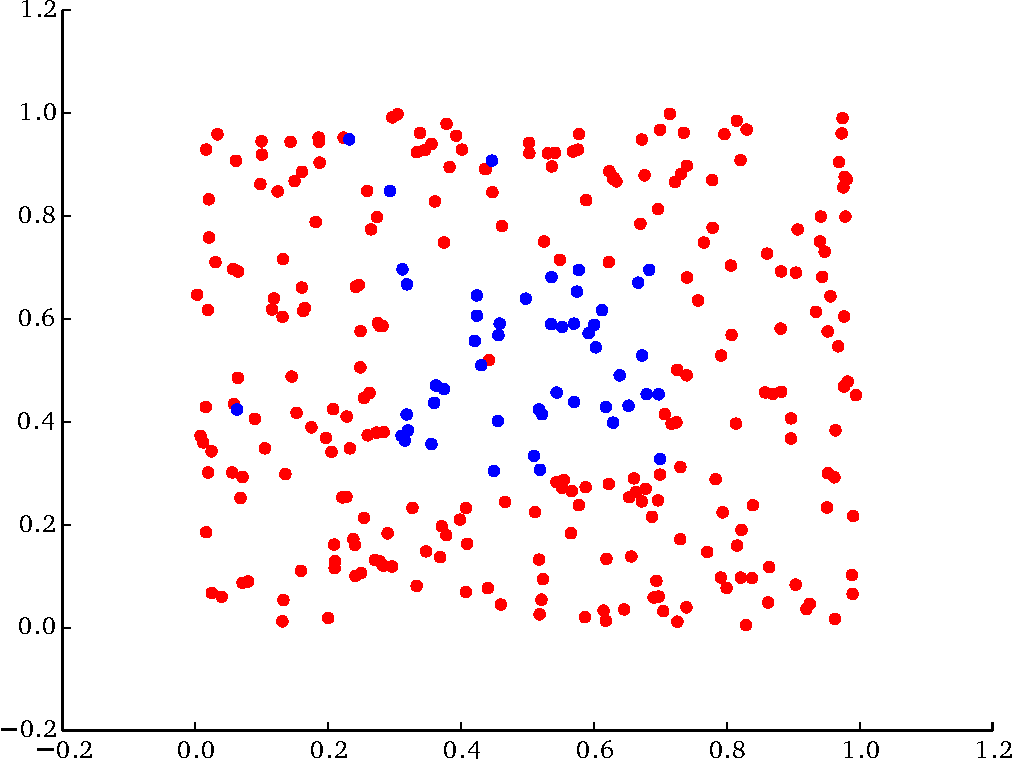
\includegraphics[width=\textwidth]{figures/ch5_learningset.pdf}
    \caption{Binary classification task.}
    \label{fig:5:set}
\end{minipage}\hfill
\begin{minipage}{0.45\textwidth}
\centering
    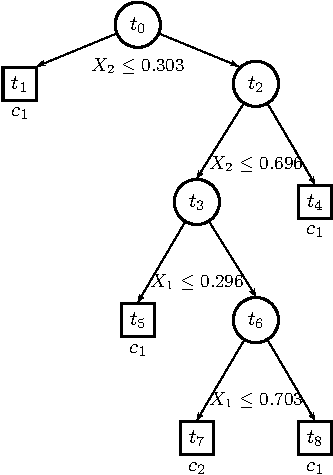
\includegraphics[scale=1.0]{figures/ch5_tree.pdf}
    \caption{Decision tree learned from Figure~\ref{fig:5:set}.}
    \label{fig:5:tree}
\end{minipage}
\end{figure}

\begin{table}
    \small
    \hspace{-1.3cm}
    \begin{tabular}{| l | c c c c c c c c c |}
    \hline
    \texttt{t}    & 0 & 1 & 2 & 3 & 4 & 5 & 6 & 7 & 8 \\
    \hline
    \hline
    \texttt{left\_child} & 1 & -- & 3 & 5 & -- & -- & 7 & -- & -- \\
    \texttt{right\_child} & 2 & -- & 4 & 6 & -- & -- & 8 & -- & -- \\
    \texttt{feature} & 2 & -- & 2 & 1 & -- & -- & 1 & -- & -- \\
    \texttt{threshold} & 0.303 & -- & 0.696 & 0.296 & -- & -- & 0.703 & -- & -- \\
    \texttt{impurity} & 0.273 & 0. & 0.368 & 0.482 &  0.065 &  0.051 & 0.48  & 0.042 &  0. \\
    \texttt{n\_samples} & 300 & 99  & 201 & 113  & 88  & 38  & 75  & 46  & 29\\
    \texttt{value} & 251/49 & 99/0 & 152/49 & 67/46 & 85/3 & 37/1 & 30/45 & 1/45 & 29/0 \\
    \hline
    \end{tabular}
    \caption{Array representation of the decision tree in Figure~\ref{fig:5:tree}.}
    \label{table:tree-array}
\end{table}

As an example, Table~\ref{table:tree-array} illustrates the array
representation of the decision tree shown in Figure~\ref{fig:5:tree}, as built
from the learning set ${\cal L}$ of Figure~\ref{fig:5:set}. Internal nodes
($t_0$, $t_2$, $t_3$ and $t_6$) are nodes for which the corresponding values in
$\texttt{left\_child}$, $\texttt{right\_child}$, $\texttt{feature}$ and
$\texttt{threshold}$ are not empty, while leaves ($t_1$, $t_4$, $t_7$ and
$t_8$) correspond to nodes for which these values are not defined. In the case
of classification, the \texttt{value} array contains the number of samples of
each class for each node. From these, class probability estimates $p_{\cal
L}(Y=c|t)$ can be computed by dividing \texttt{value[t][c]} by the number of
samples $\texttt{n\_samples[t]}$ in $t$. In the case of regression,
\texttt{value[t]} would  contain the average output value for the samples in
$t$. Finally, let us note that storing node impurities in the \texttt{impurity}
array is not strictly necessary, since these values are only used during
construction. Yet, storing them can prove to be valuable, e.g., for
later inspection of the decision tree or for computing variable importances (see
Chapter~\ref{ch:importances}) more readily.

By implementing the array representation as dynamic tables~\citep{cormen:2001},
insertion of new nodes has an $O(1)$ amortized cost, while keeping memory
allocations at a minimum and thereby reducing the overhead that would otherwise
occur using per-node data structures. Maintaining the representation
contiguously in memory also brings the benefits of leveraging CPU caches,
which might greatly improve performance when fast predictions are critical.
Since nodes are accessed successively and repeatedly at test time,
storing them in nearby memory locations is indeed recommended to improve
cache performance.

\subsection{Builders}

The implementation of the induction procedure in Scikit-Learn revolves around
three nested components:

\begin{enumerate}
\item The first component is a \texttt{Builder} object whose role is to
    effectively build the tree array representation presented above,
    by recursively partitioning nodes using splits found by a \texttt{Splitter} object.

\item The second component is a \texttt{Splitter} object whose role is to find splits on internal nodes.

\item The third component is a \texttt{Criterion} object whose role is to evaluate
    the goodness of a split.
\end{enumerate}

The most direct \texttt{Builder} implementation is the depth-first greedy
induction procedure as originally outlined in Algorithm~\ref{algo:induction}. A
critical aspect of this algorithm is how to keep account of the  the input
samples $(\mathbf{x}_i,y_i) \in {\cal L}_t$  that arrive at node $t$. A
straightforward solution is to store lists of indices of the input samples at
node $t$. As pointed out in \citep{criminisi:2013}, building many such lists is
however inefficient because of repeated memory allocations and deallocations. A
better solution is to have instead all indices stored in a single static array
and to use in-place reordering operations when partitioning $t$. More
specifically, let assume that  $\texttt{samples}$ is the list of all indices
and that  $\texttt{start}$ and $\texttt{end}$ are bounds such that
$\texttt{samples[start:end]}$ contains the sample indices at the current node
$t$. If $\texttt{t}$ is split on feature $\texttt{feature[t]}$ and threshold
$\texttt{threshold[t]}$, then ${\cal L}_t$ can be partitioned into ${\cal
L}_{t_L}$ and ${\cal L}_{t_R}$ by reorganizing $\texttt{samples[start:end]}$
into $\texttt{samples[start:pos]}$ and $\texttt{samples[pos:end]}$, such that
all samples in the first part are on the left side of the split while all
samples in the second part are on the right side of the split. The induction
procedure then proceeds by pushing the bounds $\texttt{start:pos}$ and
$\texttt{pos:end}$ on the stack $S$, as an effecient way to effectively
represent ${\cal L}_{t_L}$ and ${\cal L}_{t_R}$.

An alternative implementation of the $\texttt{Builder}$ interface consists in
replacing the stack $S$ in Algorithm~\ref{algo:induction} by a priority queue,
hence changing the order in which the nodes are split. In particular, if nodes
$t$ are prioritized by weighted potential impurity decrease $p(t) \Delta
i(s^*,t)$ (where $s^*$ is the best split on $t$), then the greedy induction
procedure switches from a depth-first construction of the tree to a \textit
{best-first} induction procedure. In this way, an additional stopping criterion
can be defined as the maximum number \texttt{max\_leaf\_nodes} of leaves in the
tree. If nodes are expanded in best-first order, then the resulting tree only
includes the most significant splits, thereby pre-pruning all (seemingly)
irrelevant branches without wasting computational resources.

Likewise,  the stack $S$ in Algorithm~\ref{algo:induction} can be replaced by a
deque data structure, in which case the induction procedure switches to a
\textit{breadth-first} construction of the tree. With some modifications,
breadth-first construction shows to be more efficient when it is expensive to
randomly access the data~\citep{criminisi:2013}, e.g., when data are too big to
fit into memory and must be streamed from disk. Breadth-first induction also
proves to be an efficient strategy when combined with parallelism, e.g., for
building a whole level of the decision tree simultaneously using multiple
cores~\citep{liao:2013}.

\subsection{Splitters}

In Scikit-Learn, \texttt{Splitter} objects implement search procedures for
finding splits on internal nodes. In the case of decision trees, they implement
algorithms~\ref{algo:findsplit} and \ref{algo:findsplit:x_j} for finding the
best split over all $p$ input variables. In the case of randomized trees, they
implement the search procedure \ref{algo:findsplit:random} over $K \leq p$
randomly drawn input variables, combined with either algorithm
\ref{algo:findsplit:x_j}, \ref{algo:findsplit:pert} or  \ref{algo:findsplit:et}
to respectively obtain Random Forests, Perfect Random Tree Ensembles or
Extremely Randomized Trees.



%        + use fortran ordering to maximize caching effects

%        + Sorting algorithms

%        + Approximately best splits
%             + Binning
%             + Subsampling

% %     - Shared computations
% %         > Splitters
% %             - (Independent splitters)
% %             - Pre-sorting + data reorganization (Breiman's strategy)
% %             - Pre-sorting + sample_mask
% %         > Multi-threading


\subsection{Criteria}

% gini , etc


\section{Benchmarks}
\label{sec:5:benchmarks}

% * Comparison of existing implementations
%     - Experiments and/or implementation details

%         List existing implementations and mention in which complexity they
%         fall in (eg., in a Table).

%         Open-source
%         * C4.5
%         * CART => Breiman Fortran code
%         * TMVA !!
%         * Scikit-Learn
%         * Weka
%             + original
%             + fast-random-forest
%         * randomForest (R)
%             + original
%             + PARF
%         * party (R)
%         * Pierre
%         * OpenCV
%         * H2O
%         * clus (Leuven)

%         Closed source
%         * Sherwood (Criminisi)
%         * WiseRF
%         * Random jungle


\cleardoublepage
%\ctparttex{}
\part{Interpreting Random Forests}\label{part:2}
\chapter{Variable importances}\label{ch:importances}

\begin{remark}{Outline}
This chapter studies variable importance measures as computed from forests of
randomized trees. In Section~\ref{sec:6:importances}, we first present how
random forests can be used to assess the importance of input variables.  We
then derive in Section~\ref{sec:6:theory} a characterization in asymptotic
conditions and show that variable importances derived from totally randomized trees
offer a three-level decomposition of the information jointly  contained in the
input variables about the output. In Section~\ref{sec:6:variable-relevance}, we
show that this  characterization only depends on the relevant variables and
then discuss these ideas in Section~\ref{sec:6:variants} in the context of
variants closer to the Random Forest algorithm. Finally, we illustrate these
results on an artifical problem in Section~\ref{sec:6:illustration}.
\end{remark}

An important task in many scientific fields is the prediction of  a response
variable based on a set of predictor variables. In many situations though, the
aim is not only to make the most accurate predictions of the response but also
to identify which predictor variables are the most important to make these
predictions, e.g. in order to understand the underlying process. Because of
their applicability to a wide range of problems and their capability to both
build accurate models and, at the same time, to provide variable importance
measures, random forests have become a major data analysis tool used with
success in various scientific areas.

Despite their extensive use in applied research, only a couple of works have
studied the theoretical properties and statistical mechanisms of these
algorithms. \citet{zhao:2000}, \citet{breiman:2004},
\citet{biau:2008,biau:2012}, \citet{meinshausen:2006} and \citet{lin:2006}
investigated simplified to very realistic variants of these algorithms and
proved  the consistency of those variants. Little is known however regarding
the variable importances computed by random forests, and -- as far as we know
-- the work of~\citet{ishwaran:2007} is indeed the only theoretical study of
tree-based variable importance measures. In this chapter, we aim at filling
this gap and present a theoretical  analysis of the Mean Decrease Impurity
importance derived from ensembles of randomized trees.

% A forest of trees is impenetrable
% as far as simple interpretations of its mechanims go~\citep{breiman:2001}.


\section{Variable importances}
\label{sec:6:importances}

% surrogates
% in ensembles
% permutation

\section{Theoretical study}
\label{sec:6:theory}


\section{Relevance of variables}
\label{sec:6:variable-relevance}


\section{Variable importances in random forest variants}
\label{sec:6:variants}


\section{Illustration}
\label{sec:6:illustration}


\chapter{Further insights from importances}\label{ch:applications}

\begin{remark}{Outline}
In this chapter, we build upon results from Chapter~\ref{ch:importances} to
further study variable importances as computed from random forests. In
Section~\ref{sec:7:redundant}, we first examine importances for variables that
are redundant. In Section~\ref{sec:7:bias}, we revisit variable importances in
the context of binary decision trees and ordered variables. In this framework, we
highlight various sources of bias that may concurrently happen when
importances are computed from actual random forests. Finally, we present in
Section~\ref{sec:7:applications} some successful applications
of variable importance measures.
\end{remark}

\noindent\textbf{Caution.} \textit{The work presented in
this chapter is exploratory. Conlusions should be considered with a grain of salt, until
further empirical verifications.}

\section{Redundant variables}
\label{sec:7:redundant}

In most machine learning problems, it is typical for input variables to be
correlated, at least to some extent, and to share common bits of information.
In image classification for instance, pixels are usually highly correlated and
individually represent nearly the same information as their neighbors. In that
sense, variables are often \textit{partially redundant}, i.e., some of the
variables may share some of the same information about the output variable $Y$.
In the extreme case, redundancy is \textit{total}  or \textit{complete}, with
some of the variables redundantly conveying exactly the same information with
respect to the output variable $Y$. In this section, we study redundancy in
random forests and show that it may have a significant effect on both the
accuracy of the ensemble and variable importance measures.

As a guiding example for our discussion, let us consider a set of input
variables and let us discuss the effect of adding redundant variables on the
structure of randomized trees. Intuitively, two variables $X_i$ and $X_j$ are
redundant if one can perfectly explains the other and vice-versa. Formally, we
define redundancy as follows:

\begin{definition}
Two variables $X_i, X_j$ are \emph{totally redundant} if no additional information
is required for describing $X_i$ given $X_j$ and vice-versa. I.e., if
\begin{equation}
H(X_i|X_j) = H(X_j|X_i) = 0.
\end{equation}
\end{definition}

In particular, a variable $X_j$ and its copy, denoted $X_j^\prime$, are totally
redundant. With respect to random forests, adding copies of variables (e.g.,
duplicating $X_j$, hence resulting in a new set of $p+1$ input variables) has
no effect when the selection of the split is deterministic (e.g., in RF for $K$
set to the maximum value). No matter the number of totally redundant variables,
the best split that is selected is always the same, even if the same splits
need to be recomputed multiple times due to redundancy. When the choice of the
best split is stochastic however (e.g., for $K$ strictly smaller than the total number
of variables), adding multiple copies of a variable $X_j$ results in
splits that may be biased towards this variable (or one of its copies), which
in turn may have a significant effect on the resulting accuracy of the
ensemble. For a fixed value of $K$, it is indeed not difficult to see that
adding copies of $X_j$ increases the probability of $X_j$, or of one of its
copies, to be in the random subset of $K$ input variables on which to look for
splits. As a corollary, it therefore also simultaneously decreases the
probability of any of the others to be selected, hence biasing
the structure of resulting decision trees. Note that the resulting net effect
on accuracy depends on the nature of duplicated variable. If $X_j$ is very
informative with respect to the input, then favoring splits on $X_j$ by
adding copies may result in an increase of accuracy. By contrast, if $X_j$
is irrelevant, then adding  copies increases the risk of overfitting.

With respect to variable importances, the effect of adding redundant variables
can be derived both qualitatively and quantitatively using results from
Chapter~\ref{ch:importances}. From Theorem~\ref{thm:relevant}, we already know
that adding irrelevant variables does not change the resulting variable
importances. Adding copies of a relevant variable however, has an effect on
both the importance of the duplicated variable and on the importance of the
remaining variables. As in the previous chapter, let us assume a set $V= \{X_1,
..., X_p\}$  of categorical input variables and a categorical output $Y$, for
which we derive the MDI importance, as computed from totally randomized and
fully developed trees built on an infinitely large dataset.

\begin{lemma}\label{lemma:red1}
Let $X_i$ and $X_j$ be totally redundant variables. For any conditioning set
$B$,
\begin{align}
& I(X_i;Y|B,X_j) = I(X_j;Y|B, X_i) = 0 \label{lemma:red1:eqn1} \\
& I(X_i;Y|B) = I(X_j;Y|B) \label{lemma:red1:eqn2}.
\end{align}
\end{lemma}

\begin{proof}
By symmetry of the mutual information, it comes
\begin{align}
I(X_i;X_j) &= H(X_i) - H(X_i|X_j) \nonumber \\
           &= H(X_j) - H(X_j|X_i),
\end{align}
which implies that $H(X_i) = H(X_j)$ since $H(X_i|X_j) = H(X_j|X_i) = 0$ if
$X_i$ and $X_j$ are totally redundant. Since $0 \leq H(X_i|X_j,B) \leq
H(X_i|X_j)$ and $H(X_i|X_j)=0$, we also have $H(X_i|X_j,B)=0$ for any conditioning
set $B$. Likewise, $H(X_j|X_i,B)=0$. By reusing the same argument for $I(X_i;X_j|B)$, equality
therefore extends to any conditioning set $B$, giving $H(X_i|B) = H(X_j|B)$.

From these, it follows that,
\begin{align}
& I(X_i;Y|B,X_j) = H(X_i|B, X_j) - H(X_i|B,X_j,Y) = 0 - 0, \\
& I(X_j;Y|B,X_i) = H(X_j|B, X_i) - H(X_j|B,X_i,Y) = 0 - 0,
\end{align}
which proves Equation~\ref{lemma:red1:eqn1}. We also have
\begin{align}
I(X_i;Y|B) &= H(X_i|B) - H(X_i|B,Y) \\
           &= H(X_j|B) - H(X_j|B,Y) \\
           &= I(X_j;Y|B),
\end{align}
which proves Equation~\ref{lemma:red1:eqn2}.
\end{proof}

\begin{proposition}\label{prop:red:self}
Let $X_j\in V$ be a relevant variable with respect to $Y$ and $V$ and let
$X_j^\prime \notin V$ be a totally redundant variable with respect to $X_j$.
The infinite sample size importance of $X_j$ as computed with an infinite
ensemble of fully developed totally randomized trees built on $V\cup
\{X_j^\prime\}$ is
\begin{equation}
\text{Imp}(X_j) = \sum_{k=0}^{p-1} \frac{p-k}{p+1} \frac{1}{C_p^k} \frac{1}{p-k} \sum_{B \in {\cal P}_k(V^{-j})} I(X_j;Y|B)
\end{equation}
\end{proposition}

\begin{proof}
From Theorem~\ref{thm:imp}, the variable importance of $X_j$ is
\begin{align}
\text{Imp}(X_j) &= \sum_{k=0}^{p-1+1} \frac{1}{C_{p+1}^k} \frac{1}{p+1-k} \sum_{B \in {\cal P}_k(V^{-j} \cup \{X_j^\prime\})} I(X_j;Y|B) \nonumber \\
&= \sum_{k=0}^{p-1} \frac{1}{C_{p+1}^k} \frac{1}{p+1-k} \sum_{B \in {\cal P}_k(V^{-j})} I(X_j;Y|B) \nonumber \\
&= \sum_{k=0}^{p-1} \frac{p-k}{p+1} \frac{1}{C_{p}^k} \frac{1}{p-k} \sum_{B \in {\cal P}_k(V^{-j})} I(X_j;Y|B),
\end{align}
since from Lemma~\ref{lemma:red1}, $I(X_j;Y|B\cup X_j^\prime)=0$ for all $B \in {\cal P}(V^{-j})$.
\end{proof}

\begin{lemma}\label{lemma:red2}
Let $X_i$ and $X_j$ be totally redundant variables. For any conditioning set
$B$ and for any variable $X_l$,
\begin{equation}
I(X_l;Y|B,X_i) = I(X_l;Y|B, X_j) = I(X_l;Y|B, X_i, X_j) \label{lemma:red2:eqn}
\end{equation}
\end{lemma}

\begin{proof}
From the chaining rule of the mutual information, we have
\begin{align}
I(X_i,X_j,X_l;Y|B) &= I(X_l;Y|B) + I(X_i,X_j;Y|B,X_l) \nonumber \\
                   &= I(X_l;Y|B) + I(X_i;Y|B,X_l) + I(X_i;Y|B, X_j, X_l) \nonumber \\
                   &= I(X_l;Y|B) + I(X_i;Y|B,X_l) \quad\text{(Lemma~\ref{lemma:red1})} \nonumber \\
                   &= I(X_i, X_l;Y|B) \nonumber \\
                   &= I(X_i;Y|B) + I(X_l;Y|B,X_i) \label{lemma:red2:eqn1}.
\end{align}
By symmetry,
\begin{equation}\label{lemma:red2:eqn2}
I(X_i,X_j,X_l;Y|B) = I(X_j;Y|B) + I(X_l;Y|B,X_j),
\end{equation}
which proves that $I(X_l;Y|B,X_i) = I(X_l;Y|B, X_j)$, by combining both equations
and using the fact that $I(X_i;Y|B) = I(X_j;Y|B)$ (Lemma~\ref{lemma:red1}).

From the chaining rule, we also have
\begin{align}
I(X_i,X_j,X_l;Y|B) &= I(X_i, X_j;Y|B) + I(X_l;Y|B,X_i,X_j) \nonumber \\
                   &= I(X_i; Y|B) + I(X_j;Y|B, X_i) + I(X_l;Y|B,X_i,X_j) \nonumber \\
                   &= I(X_i; Y|B) + I(X_l;Y|B,X_i,X_j).
\end{align}
By combining this last equation with Equation~\ref{lemma:red2:eqn1},
we finally have $I(X_l;Y|B,X_i) = I(X_l;Y|B,X_i,X_j)$, which proves
Lemma~\ref{lemma:red2}.
\end{proof}

\begin{proposition}\label{prop:red:other}
Let $X_j\in V$ be a relevant variable with respect to $Y$ and $V$ and let
$X_j^\prime \notin V$ be a totally redundant variable with respect to $X_j$.
The infinite sample size importance of $X_l \in V^{-j}$ as computed with an infinite
ensemble of fully developed totally randomized trees built on $V\cup
\{X_j^\prime\}$ is
\begin{align}\label{prop:red:other:eqn}
\text{Imp}(X_l) &= \sum_{k=0}^{p-2} \frac{p-k}{p+1} \frac{1}{C_p^k} \frac{1}{p-k} \sum_{B \in {\cal P}_k(V^{-l} \setminus X_j)} I(X_l;Y|B) + \\
                & \hookrightarrow \sum_{k=0}^{p-2}  \left[ \sum_{k'=1}^2 \frac{C^{k'}_2}{C_{p+1}^{k+k'}} \frac{1}{p+1-(k+k')} \right]  \sum_{B \in {\cal P}_k(V^{-l}\setminus X_j)} I(X_l;Y|B\cup X_j). \nonumber
\end{align}
\end{proposition}

\begin{proof}
From Lemma~\ref{lemma:red2}, conditioning by either $X_j$, $X_j^\prime$ or by
both  variables yield terms $I(X_l;Y|B,X_j)$, $I(X_l;Y|B,X_j^\prime)$ and
$I(X_l;Y|B,X_j,X_j^\prime)$ that are all equal. From Theorem~\ref{thm:imp}, the
variable importance of $X_l$ can therefore be rewritten as follows:

\begin{align}
\text{Imp}(X_l) &= \sum_{k=0}^{p-1+1} \frac{1}{C_{p+1}^k} \frac{1}{p+1-k} \sum_{B \in {\cal P}_k(V^{-l}\cup X_j^\prime)} I(X_l;Y|B) \nonumber \\
           &= \sum_{k=0}^{p-2} \sum_{k'=0}^2 \frac{1}{C_{p+1}^{k+k'}} \frac{1}{p+1-(k+k')} \sum_{\substack{B \in {\cal P}_k(V^{-l} \setminus X_j)\\ B' \in {\cal P}_{k'}(\{X_j, X_j^\prime\})} } I(X_l;Y|B \cup B') \nonumber \\
           &= \sum_{k=0}^{p-2} \frac{1}{C_{p+1}^k} \frac{1}{p+1-k} \sum_{B \in {\cal P}_k(V^{-l} \setminus X_j)} I(X_l;Y|B) + \nonumber \\
           & \hookrightarrow \sum_{k=0}^{p-2} \left[ \sum_{k'=1}^2 \frac{C^{k'}_2}{C_{p+1}^{k+k'}} \frac{1}{p+1-(k+k')} \right] \sum_{B \in {\cal P}_k(V^{-l} \setminus X_j)} I(X_l;Y|B \cup X_j) \nonumber \\
           &= \sum_{k=0}^{p-2} \frac{p-k}{p+1} \frac{1}{C_p^k} \frac{1}{p-k} \sum_{B \in {\cal P}_k(V^{-l} \setminus X_j)} I(X_l;Y|B) + \nonumber \\
           & \hookrightarrow \sum_{k=0}^{p-2}  \left[ \sum_{k'=1}^2 \frac{C^{k'}_2}{C_{p+1}^{k+k'}} \frac{1}{p+1-(k+k')} \right]  \sum_{B \in {\cal P}_k(V^{-l}\setminus X_j)} I(X_l;Y|B\cup X_j). \nonumber
\end{align}
\end{proof}

Proposition~\ref{prop:red:self} shows that the importance of $X_j$ decreases
when a redundant variable $X_j^\prime$ is added to the set of input variables,
since all mutual information terms are multiplied by a factor $\tfrac{p-k}{p+1}
< 1$. Intuitively, this result is in fact expected since the same information
is then conveyed within two variables (i.e., in $X_j$ and its copy
$X_j^\prime$). It also shows that the terms in the total importance are not all
modified in the same way. The weight of the terms corresponding to small
conditioning sets remains nearly unchanged (i.e., for a large number $p$ of
variables and small values of $k$, $\tfrac{p-k}{p+1}$ is close to $1$), while
the weight of the terms of large conditioning sets is greatly impacted (i.e.,
for large values of $k$, $\tfrac{p-k}{p+1}$ tends to $0$).

As shown by Proposition~\ref{prop:red:other}, the effect of adding a redundant
variable $X_j^\prime$ on the importance of the other variables $X_l$ (for
$l\neq j$) is twofold. The first part of Equation~\ref{prop:red:other:eqn}
shows that the weight of all terms that do not include $X_j$ (or its copy)
strictly decreases by a factor $\tfrac{p-k}{p+1}$. The second part of
Equation~\ref{prop:red:other:eqn} shows that the the weight of all terms that
include $X_j$ (or its copy) increases, since several equivalent conditioning
sets (i.e., $B\cup \{X_j\}$, $B\cup \{X_j\}^\prime$ and $B\cup \{X_j,
X_j^\prime\}$) can now appear within the branches of a tree. Like for
Proposition~\ref{prop:red:self}, impurity terms are not all modified in the
same way and changes depend on the size $k$ of the conditioning set $B$.
Overall, the net effect on the total importance of $X_l$ is therefore a
compromise between these opposing changes. If the weighted sum of the
$I(X_l;Y|B,X_j)$ terms is low with respect to the sum of the terms that do not
include $X_j$ (or its copy), then the decrease effect dominates and the
importance of $X_l$ should be smaller. By contrast, if the $I(X_l;Y|B,X_j)$
terms are larger, then the increase effect dominates and the resulting
importance is larger. As shown later in Figure~\ref{fig:7:red:xor}, redundant variables therefore
increase the importance of all variables that \textit{interact} with the duplicated variable.

Propositions~\ref{prop:red:self} and \ref{prop:red:other} can be extended to
the case where $N_c$ redundant variables $X_j^c$ (for $c=1,\dots,N_c$) are
added to the input variables instead of one, leading to the general
Proposition~\ref{prop:red:general}. From this result, the same qualitative
conclusions can drawn, except that the decrease or increase effects discussed
above are even stronger as more redundant variables are added.

\begin{proposition}\label{prop:red:general}
Let $X_j\in V$ be a relevant variable with respect to $Y$ and $V$ and let
$X_j^c \notin V$ (for $c=1,\dots,N_c$) be $N_c$ totally redundant variables with respect to $X_j$.
The infinite sample size importances of $X_j$ and $X_l \in V$ as computed with an infinite
ensemble of fully developed totally randomized trees built on $V\cup
\{X_j^1,\dots,X_j^{N_c}\}$ are
\begin{align*}
\text{Imp}(X_j)  &= \sum_{k=0}^{p-1} \left[ \frac{C^k_p (p-k)}{C^k_{p+N_c}(p+N_c-k)}  \right] \frac{1}{C_p^k} \frac{1}{p-k} \sum_{B \in {\cal P}_k(V^{-j})} I(X_j;Y|B), \\
\text{Imp}(X_l) &= \sum_{k=0}^{p-2} \left[ \frac{C^k_p (p-k)}{C^k_{p+N_c}(p+N_c-k)}  \right] \frac{1}{C_p^k} \frac{1}{p-k} \sum_{B \in {\cal P}_k(V^{-l} \setminus X_j)} I(X_l;Y|B) + \\
                & \hookrightarrow \sum_{k=0}^{p-2}  \left[ \sum_{k'=1}^{N_c+1} \frac{C^{k'}_{N_c+1}}{C_{p+N_c}^{k+k'}} \frac{1}{p+N_c-(k+k')} \right]  \sum_{B \in {\cal P}_k(V^{-l}\setminus X_j)} I(X_l;Y|B\cup X_j).
\end{align*}
\end{proposition}

\begin{proof}
Omitted here, but Proposition~\ref{prop:red:general} can be proved
by generalizing for $N_c$ the proofs of Propositions~\ref{prop:red:self}
and \ref{prop:red:other}.
\end{proof}

As an illustrative example, let us reconsider the LED classification problem
from Section~\ref{sec:6:illustration}, and for which $X_5$ was found to be the
most important variable. As shown in Figure~\ref{fig:7:red:led}, adding
variables that are redundant with $X_5$ makes its importance decrease, as
predicted by our theoretical result from Propositions~\ref{prop:red:self} and
\ref{prop:red:general}. When 5 or more copies of $X_5$ are added, the
importance of $X_5$ is the smallest of all, as if $X_5$ had become less
informative. Similarly, we observe that the importance of the other variables
remain about the same or slightly decrease, as if they all had become a bit
less informative. With regards to our previous results in Propositions
\ref{prop:red:other} and \ref{prop:red:general}, this indicates that the
importance due to the $I(X_l;Y|B)$ terms prevails from  the importance due to
the $I(X_l;Y|B,X_5^c)$ terms. As a matter of fact, this example highlights a
fundamental property of variable importances as computed in a random forest:
importance measures are computed not only with respect to the output $Y$, but
also with respect to all the other input variables that define the problem. In
particular, a variable which is not important is not necessarily uninformative,
as the example illustrates. A variable may be considered as less important
because the  information it conveys is also redundantly conveyed in other
variables, and not necessarily because it has no information.

\begin{figure}
\centering
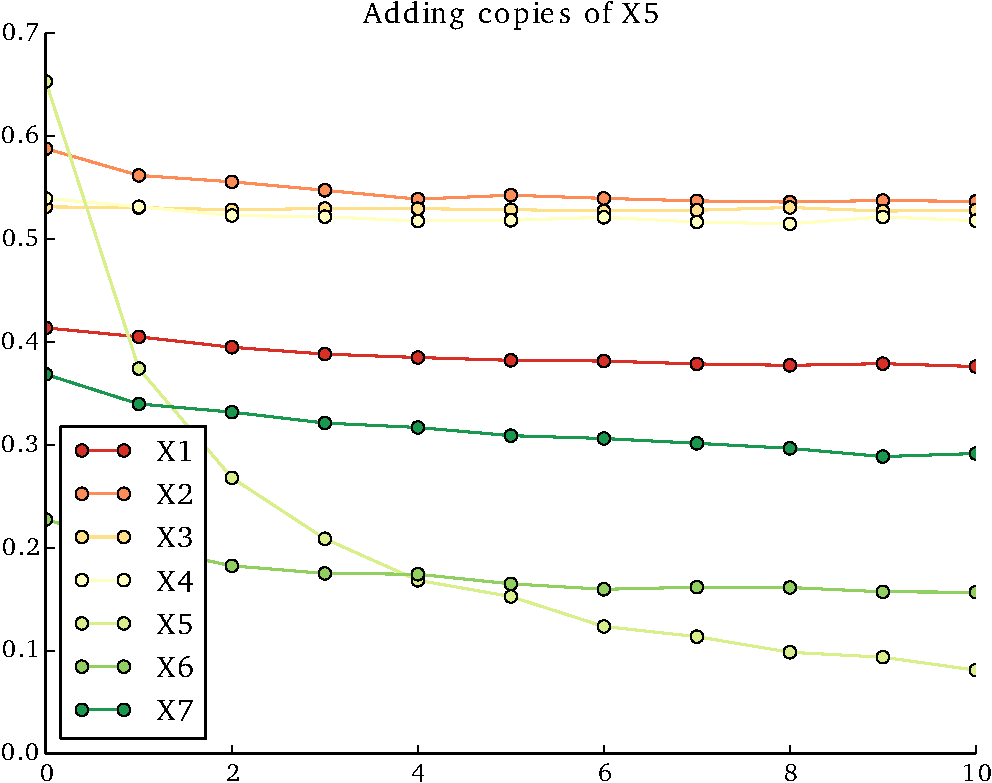
\includegraphics[width=0.9\textwidth]{figures/ch7_red_led.pdf}
\caption{Adding copies of $X_5$ on the LED classification task. The more
         redundant variables are added, the lesser the importance of $X_5$.}
\label{fig:7:red:led}
\end{figure}


\begin{figure}
\centering
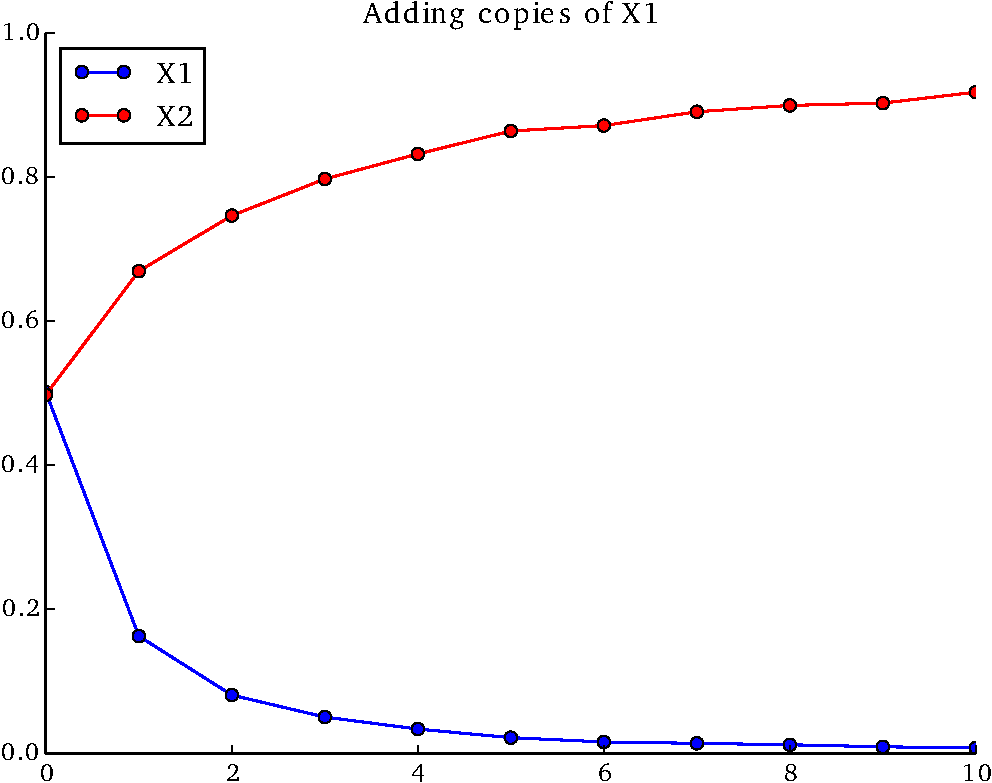
\includegraphics[width=0.9\textwidth]{figures/ch7_red_xor.pdf}
\caption{Adding copies of $X_1$ on a XOR classification task. The more redundant
         variables are added, the lesser the importance of $X_1$, but the larger
         the importance of $X_2$.}
\label{fig:7:red:xor}
\end{figure}

As a second example, Figure~\ref{fig:7:red:xor} illustrates redundancy effects
for a XOR classification problem defined on two variables $X_1$ and $X_2$.
Again, the importance of the duplicated variable $X_1$  decreases as redundant
variables are added, which confirms our results from
Propositions~\ref{prop:red:self} and \ref{prop:red:general}. More
interestingly, we now observe that the importance of the other variable, $X_2$,
increases as copies of $X_1$ are added. For this problem, the
$I(X_2;Y|B,X_1^c)$ terms are prevalent with respect to the $I(X_2;Y|B)$ terms
(which is in fact unique and equal to $0$), thereby artificially increasing the
overall importance of $X_2$ as redundancy augments, as expected from
Propositions \ref{prop:red:other} and \ref{prop:red:general}.

Overall, results presented in this section call for caution when interpreting
variable importance scores. Due to redundancy effects -- either total, as studied
here, or partial as it would often arise in practice -- it may happen that the
total importance of a given variable is either misleadingly low or deceptively
high because the same information is spread within several redundant variables
and therefore taken into account several times within the total importances. As
such, we advise to complement the interpretation with a systematic
decomposition of variable importance scores, e.g., as previously done in
Figure~\ref{fig:decomposition}, in order to better understand why a variable is
in fact important and to possibly detect redundancy.


\section{Bias in variable importances}
\label{sec:7:bias}

In this section, we study sources of bias in variable importances and show that
variable selection (as previously discussed in Section~\ref{sec:ntrt}) is  not
the only cause of bias. In practice, complementary forces due to masking
effects, impurity misestimations and the structure of the trees make variable
importances deviate from the theoretical results found in asymptotic conditions
for totally randomized trees.

\subsection{Bias due to masking effects}

As shown in the previous chapters, the guided selection of the split variable
(i.e., for $K>1$) is necessary for balancing bias and variance in  randomized
decision trees and to produce accurate ensembles. In particular, we studied
that decision trees built with too much randomization usually lead to an
increase of bias which cannot be compensated by a reciprocal decrease of
variance, making it necessary to adjust the value of $K$ to find the
appropriate trade-off. By contrast, we also showed in Section~\ref{sec:ntrt}
that when variable selection is not totally random (i.e., as soon as $K>1$),
masking effects induce a bias with respect to variable importances, since it
forces some of the branches to never be built, and therefore some of the
conditioning sets $B \in {\cal P}(V)$ to never be taken into account. As a
consequence, random forests whose parameter $K$ has been tuned to maximize
accuracy may yield variable importances that are biased (either
over- or underestimated). More specifically, it can be shown (see
Section~\ref{sec:ntrt}) that a relevant variable may be null with regards to
its importance, thereby making it indistinguishable from irrelevant variables,
and that the importance of relevant variables becomes dependent on the number
of irrelevant variables.


\subsection{Bias due to impurity misestimations}
\label{sec:7:bias:high}

In many applications, input variables are heterogeneous and vary in their scale
of measurement or in the number of categories they may take. For example, in
the case of meteorelogical problems, variables often comprise mixed
environemental measurements of different nature and scale,   like speed of
wind, temperature, humidity, pressure, rainfall or solar radidation. As we show
in this section, misestimations of node impurity is in fact directly
proportional to the cardinality of the split variable and inversely
proportional to the number $N_t$ of samples used for the evaluation. As a
result, impurity reductions become overestimated as we go deeper in the tree
and/or as the number of values of the variable is large. In this context,
variable importances suffer from bias, making variables of higher cardinality
wrongly appear as more important.

To guide our discussion, let us revisit the simulation studies from
\citep{strobl:2007b} which consider a binary output variable $Y$ and five
input variables $X_1,\dots,X_5$, as defined in Table~\ref{table:simulation}.

\begin{table}
    \centering
    \begin{tabular}{| c c c |}
    \hline
    & $X_1$ & $\sim{\cal N}(0, 1)$ \\
    & $X_2$ & $\sim{\cal M}(2)$ \\
    & $X_3$ & $\sim{\cal M}(4)$ \\
    & $X_4$ & $\sim{\cal M}(10)$ \\
    & $X_5$ & $\sim{\cal M}(20)$ \\
    \hline
    \hline
    {\it null case}  & $Y$ & $\sim{\cal B}(0.5)$ \\
    {\it power case} & $Y|X_2=0$ &  $\sim{\cal B}(0.5-\text{relevance})$ \\
                     & $Y|X_2=1$ &  $\sim{\cal B}(0.5+\text{relevance})$ \\
    \hline
    \end{tabular}
    \caption{Input variables are independent random variables as defined from
    the table. ${\cal N}(0, 1)$ is the standard normal
    distribution. ${\cal M}(k)$ is the multinomial distribution with values in $\{0, \dots, k-1\}$
    and equal probabilities. ${\cal B}(p)$ is the binomial distribution. In the
    null case, $Y$ is independent from $X_1, \dots, X_5$. In the power case, $Y$
    depends on the value $X_2$ while other input variables remain irrelevant.}
    \label{table:simulation}
\end{table}

\begin{figure}
\centering
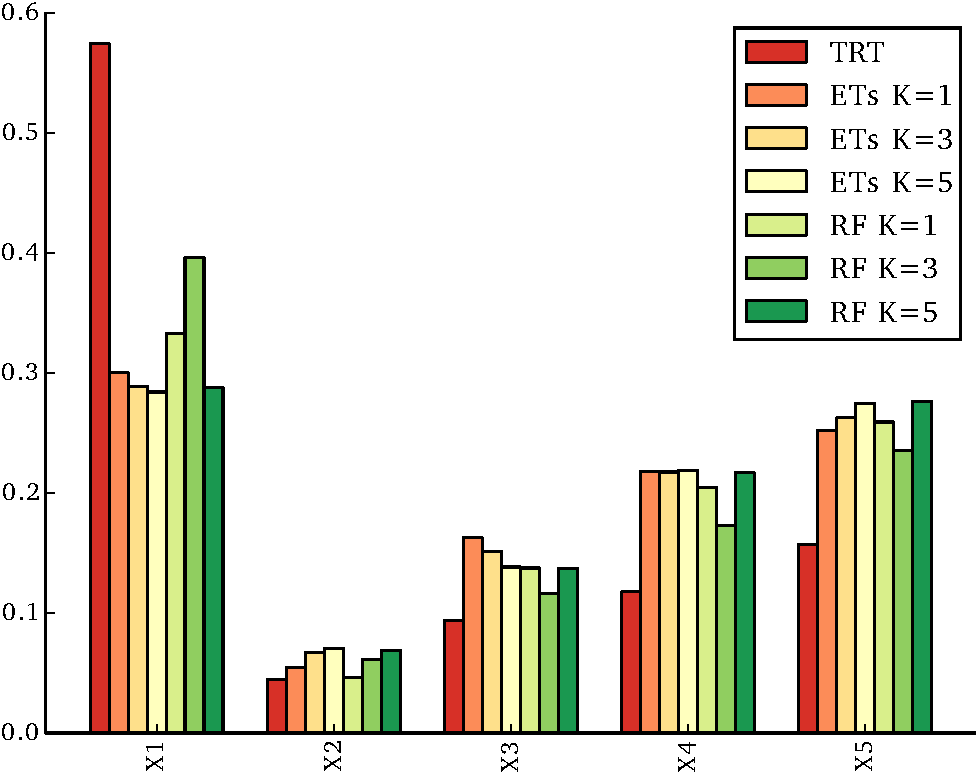
\includegraphics[width=0.9\textwidth]{figures/ch7_bias_null.pdf}
\caption{Variable importances for $Y$ independent of $X_1, \dots, X_5$. ($N=120$, $M=500$)}
\label{fig:7:bias:null}
\end{figure}

Let us first analyze the case where $Y$ is independent from $X_1, \dots, X_5$,
i.e., such that none of the input variables are informative with respect to the
output. For a randomly sampled dataset ${\cal L}$ of $N=120$ samples,
Figure~\ref{fig:7:bias:null} plots variable importances for different kinds of
random forests. TRT corresponds to totally randomized trees, as defined in
Section~\ref{sec:6:theory}, RF corresponds to standard Random Forest with
bootstrap sampling and ETs corresponds to Extremely Randomized Trees. Both RF
and ETs use binary splits while TRT rely on multiway exhaustive
splits\footnote{Thereby creating as many branches as the number of values of
the split variable, even if this variable is continuous and count unique values
only.}. In asymptotic conditions, we proved in Theorem~\ref{thm:irrelevant}
that the importance of irrelevant variables is strictly equal to $0$. For a
finite value of $N$ however, this result does not hold, as
Figure~\ref{fig:7:bias:null} indeed confirms. In contrast with what would be
expected, we observe that the importance of none of the variables is in fact
nowhere close to $0$. In light of Theorem~\ref{thm:sum-of-imp} however, this
result is not that surprising: as long as decision trees can be fully
developed, the sum of variable importances is equal to  the (empirically
estimated) mutual information between $X_1,\dots,X_p$ and the output $Y$, which
is itself upper bounded by the (empirically estimated) entropy $H(Y)$ of the
output variable. In this case, $H(Y)=\log_2(2)=1$, which indeed corresponds to
the sum of variable importances for all methods compared in the figure. More
importantly, we also observe that the larger the cardinality of the variable
(i.e., the larger its number of unique values), the larger its importance. For
example, the importance of $X_1$ (for which samples all have unique values) or
of $X_5$ (which counts up to $40$ unique values) appears nearly $3$ times
larger as the importance of $X_2$ (which is binary).

In their study, \citet{strobl:2007b} argue that this bias is due to variable
selection: \textit{variables with more potential cut-points are more likely to
produce a good criterion value by chance, as in a multiple testing situation}.
As a result, variables of higher cardinality are more likely to be chosen for
splitting than those of lower cardinality. While this bias has been known for
long in decision trees~\citep{kononenko:1995,kim:2001,hothorn:2006}, we argue
that it is not the actual cause for the bias observed here. Indeed, this
argument does not directly explain why similar trends are also observed when no
variable selection is performed (e.g., for TRT or for $K=1$) nor why it
similarly happens when cut-points are chosen at random, independently of the
cardinality of the variable (e.g., in ETs).

For multiway splits like in TRT, bias in variable importances can be traced to the
misestimations of the mutual information terms
\begin{equation}
\Delta i(s, t) \approx I(X_j;Y|t)
\end{equation}
due to the finite size $N_t$ of the node samples. As shown in
\citep{goebel:2005}, when $X_j$ and $Y$ are independent random variables (i.e.,
when $X_j$ is irrelevant), the distribution of finite sample size estimates of
their mutual information  follows approximately a gamma distribution
\begin{equation}
\widehat{I}(X_j; Y) \sim \Gamma\Big( \frac{1}{2}(|{\cal X}_j|-1)(|{\cal Y}|-1), \frac{1}{N_t \log 2} \Big)
\end{equation}
whose mean is linearly proportional to the cardinalities $|{\cal X}_j|$ and
$|{\cal Y}|$ of $X_j$ and $Y$ and inversely proportional to $N_t$:
\begin{equation}
\mathbb{E}\{ \widehat{I}(X_j; Y) \} = \frac{(|{\cal X}_j|-1)(|{\cal Y}|-1)}{2 N_t \log 2}.
\end{equation}
As a result, estimates get larger as $X_j$ counts many unique values, and
become even larger as nodes are deep in the tree (since $N_t$ gets smaller).
Consequently, the weighted mean of all such estimated impurity terms
$I(X_j;Y|t)$, for all nodes $t$ where $X_j$ is the split variable, and
resulting in the total importance $\text{Imp}(X_j)$, is also linearly dependent
on the cardinality of $X_j$. For TRT, this result explains why variables of
high cardinality in Figure~\ref{fig:7:bias:null} appear as more important than
those of lower cardinality. Intuitively, the closer the number of unique values
with respect to the total number of samples, the larger the impurity decrease
when splitting exhaustively on this variable. In the extreme case, when values
for $X_j$ are all unique, splitting on the variable perfectly memorizes the
values of $Y$, resulting in child nodes that are all pure, therefore maximizing
the estimated mutual information. As such, this explains why $X_1$, whose
values are all unique, appears as the most important variable.

For binary splits (i.e., for RF and ETs, but not for TRT) the mutual
information $I(X_j;Y|t)$ is not directly estimated at each node. Rather, in the
case of ordered variables, $\Delta i(s, t)$ corresponds to an estimate of the
mutual information $I(X_j\leq v;Y|t)$ of the binary split $X_j \leq v$. Under
the simplifying assumption that binary splits on the same variable are all
directly consecutive in the decision tree,  it is easy to see that recursive
binary partitioning eventually ends up emulating direct multiway exhaustive
splits, as illustrated in Figure~\ref{fig:7:splits}. Using an argument similar
to the proof of Theorem~\ref{thm:sum-of-imp}, intermediate impurity terms
between the first split and the last of those splits cancel each other when
summing up the importances, which finally amounts to collect an actual estimate
of $I(X_j;Y|t)$ from the sequence of binary splits. For the same reasons as before,
variables of high cardinality are therefore biased in the same way. (As we will
study in Section~\ref{sec:bias:tree}, this assumption does not hold in
practice, making the importances from binary decision trees strictly different
from those of multiway decision trees. Yet, the qualitative conclusions are
still valid since variables of high cardinality can be reused far more many
times than variables of low cardinality, before all possible splits are
exhausted.)

\begin{figure}
    \centering
    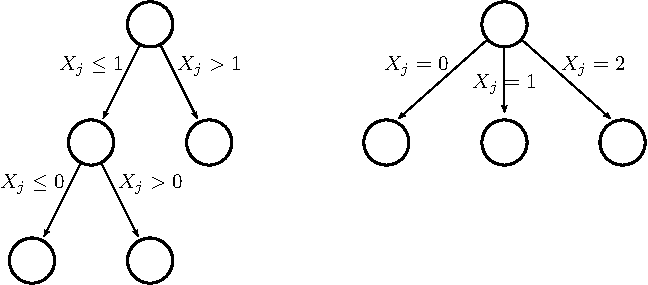
\includegraphics[scale=1.0]{figures/ch7_splits.pdf}
    \caption{Consecutive binary splits on the same variable are equivalent to direct multiway splits.}
    \label{fig:7:splits}
\end{figure}

In both situations, the origin of the problem stems from the fact that node
impurity is misestimated when the size $N_t$ of the node samples is too small.
To a large extent, the issue is aggravated by the fact that trees are fully
developed by default, making impurity terms collected near the leaves usually
unreliable. As a precaution, a safe and effective solution for the bias problem
therefore simply consists in collecting impurity terms only for those nodes
where the impurity estimates can be considered as reliable. Equivalently, the
construction of the tree can also be stopped early, when impurity estimates
become unreliable, e.g., by limiting the depth of the tree, controlling for the
minimum number of samples in internal nodes or using any of the other  stopping
criteria defined in Section~\ref{sec:3:stop}. Among all alternatives,
conditional inference trees~\citep{hothorn:2006} and earlier
methods~\citep{quinlan:1986,wehenkel:1998} make use of statistical tests for
assessing the independence of $X_j$ and $Y$ at a pre-specified level of
confidence $\alpha$. If the null hypothesis cannot be rejected, then recursive
partitioning halts. In particular, variable importances collected from
conditional inference trees were shown experimentally by \citet{strobl:2007b}
not to suffer from bias. The authors argue that it is due to the unbiased
variable selection mechanisms also implemented in conditional inference trees.
By contrast, we argue that the absence of bias in importances from such trees
is mostly due to the early stopping criterion, and not to variable selection.
Although variable selection plays an important and exacerbating role, it is not
the true cause of the  observed bias. Indeed, since the impurity reduction of
variables of high cardinality is overestimated, searching for a split among
$K>1$ randomly drawn variables increases their probability of being selected
when compared to others of lower cardinality, therefore masking and reducing
the importances of these latter variables. Yet, bias stems from the fact
that impurity reductions are misestimated in the first place.

\begin{figure}
\centering
ETs without variable selection\\[1ex]
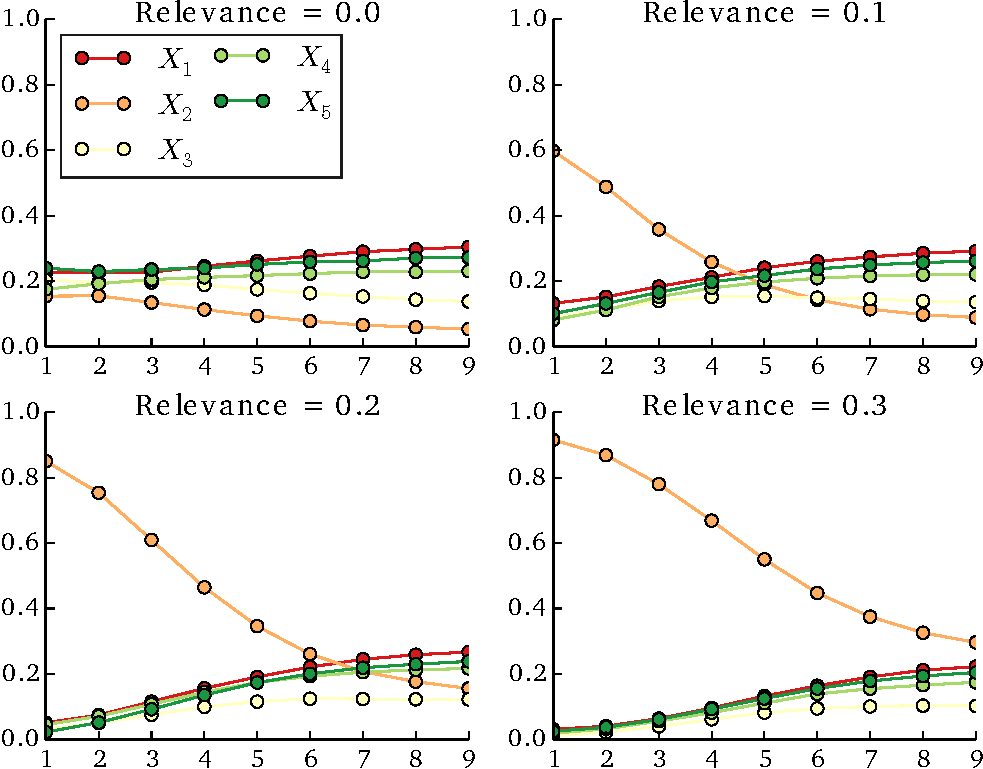
\includegraphics[width=0.9\textwidth]{figures/ch7_bias_depth.pdf}\\[2ex]
Random Forest with variable selection\\[1ex]
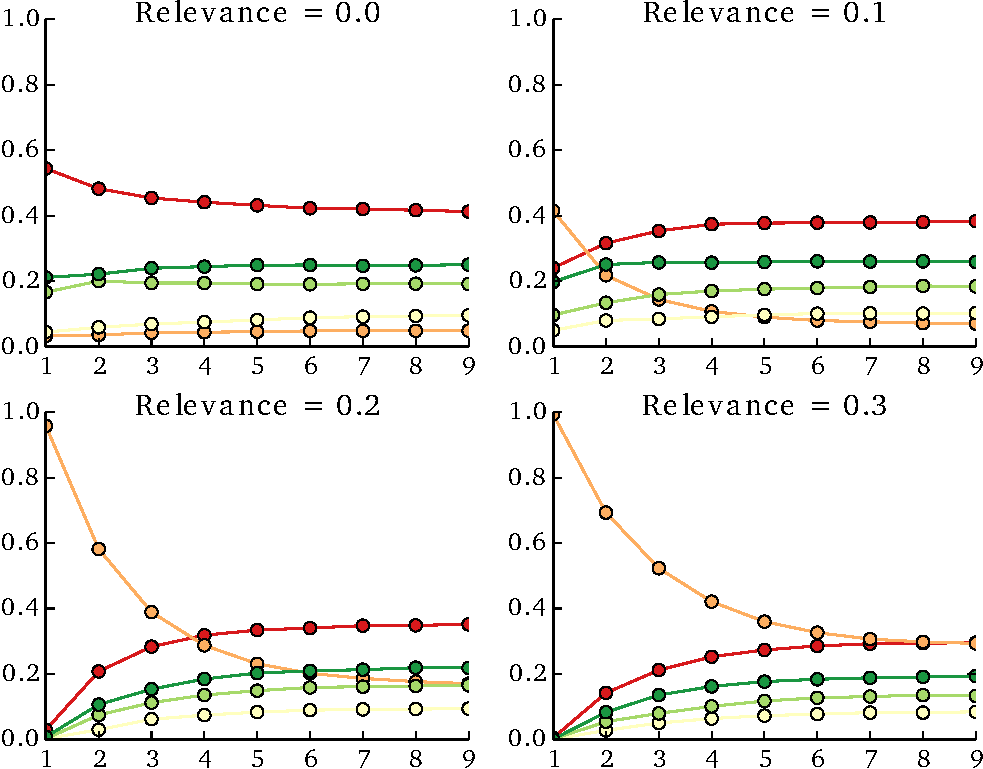
\includegraphics[width=0.9\textwidth]{figures/ch7_bias_depth_rf.pdf}
\caption{Variable importances of $X_1, \dots, X_5$ when varying both the
         maximum depth of the trees and the degree of relevance of $X_2$.
         Importance scores are normalized by the sum of importances.
         (Top) ETs with no variable selection, $K=1$, $N=120$, $M=500$.
         (Bottom) Random Forest with variable selection, $K=5$, $N=120$, $M=500$.}
\label{fig:7:bias:depth}
\end{figure}

As an illustrative example, Figure~\ref{fig:7:bias:depth} reconsiders the
simulation study of Table~\ref{table:simulation}, when varying both the maximum
depth of the trees (from $\texttt{max\_depth}=1$ to $9$) and the relevance of
$X_2$ with respect to $Y$.  Let us first consider ETs  built with no variable
selection ($K=1$), as shown in four top plots of the figure. For the null case,
when $\text{relevance}=0$, limiting the depth of the trees correctly fixes the
bias that was observed before. For shallow trees, the importances before
normalization of all five input variables are close to 0, as expected from
irrelevant variables. The normalized importances, as shown in the figure, are
also all close to $\tfrac{1}{p}=0.2$, confirming that no variable is detected
as more relevant than the others. However, when the depth of the decision trees
increases, importances deviate and bias proportional to the cardinality of the
variables appear as discussed before. When $X_2$ is a relevant variable (i.e.,
for $\text{relevance}>0$), its importance is expected to be strictly positive
and at least as large as the importances of the irrelevant variables. For
$\text{relevance}=0.1$ and $\texttt{max\_depth=1}$, the importance of $X_2$
appears nearly $6$ times larger than the importances of the other variables,
confirming that $X_2$ is correctly identified as a relevant variable.  For
deeper trees  however, noise dominates and the importance of the irrelevant
variables is larger due to misestimations of the impurity terms. As  relevance
increases, $X_2$ can more clearly be identified as a relevant variable. In
particular, the more relevant $X_2$, that is the stronger the signal, the
deeper trees can be built until $X_2$ is made unrecognizable from the
irrelevant variables.

By comparison, the four bottom plots of Figure~\ref{fig:7:bias:depth}
illustrate variable importances for RF built with variable selection ($K=5$).
Again, we observe that limiting the depth of the trees help reduce the
misestimation bias. However, the aggravating effect of variable selection is
also clearly visible: variables of larger cardinality appear as significantly
more important than the other variables. Consequently, this makes the
detection of  $X_2$ as a relevant variable more difficult when trees are grown
deeper. When comparing the relative importance of $X_2$ for a given depth and
relevance, we indeed observe that $X_2$ consistenly appears as less important
in RF than in ETs. It is only for very shallow trees ($\texttt{max\_depth=1}$
or $\texttt{2}$) and high relevance that $X_2$ is identified with higher
confidence than in ETs.

In conclusion, evaluating impurity on small samples lead to over-estimations of
the mutual information, resulting in biased variable importances. In
particular, the higher the cardinality of the variable,  the larger the
misestimations. To minimize this effect, caution should be taken by only
considering impurity terms that were computed from a large enough sample. This
can be guaranteed, e.g., by stopping the construction of the tree early, or
making leaves grow more slowly than the size $N$ of the learning set.
Additionally, we have also shown that variable selection may increase the bias
due to over-estimations. In this case, a simple remedy consists in not using
variable selection when assessing the relevance of variables.

\subsection{Bias due to binary trees and threshold selection}
\label{sec:bias:tree}

Previous developments from Chapter~\ref{ch:importances} studied variable
importances for fully developed totally randomized trees and multiway
exhaustive splits. In practice however, random forests usually rely on binary
splits rather than on multiway splits. In terms of impurity, this results in
additional and distinct information terms that were not previously accounted
for, because i) a same variable can be reused several times along the same
branch and ii) binary splits discretize the information contained in a
variable, making variable importances dependent on the split threshold selection
strategy. In lack of a rigorous theoretical framework, we give in this section
preliminary insights on variable importances for binary decision trees,
hopefully shedding some light on their interpretation.

\begin{table}
    \centering
    \begin{tabular}{| c | c c |}
    \hline
    $y$ & $x_1$ & $x_2$ \\
    \hline
    \hline
    0 & 0 & 0 \\
    1 & 1 & 1 \\
    1 & 2 & 1 \\
    \hline
    \end{tabular}
    \caption{Toy problem. All $3$ possible samples are equiprobable.}
    \label{table:simulation:bias:tree}
\end{table}

As a simplistic but illustrative example, let us consider a toy classification
problem composed of a ternary input variable $X_1$ and of a binary input
variable $X_2$, both of them being ordered. Let us further assume that input samples are uniformly drawn
from Table~\ref{table:simulation:bias:tree}, which defines the output as $Y =
X_1 < 1$ and $X_2$ as a copy of $Y$. With respect to $Y$, both variables are as
informative and one should expect their importances to be the same.  With
totally randomized trees and exhaustive splits, two equiprobable decision trees
can be built, as represented in Figure~\ref{fig:7:bias:trees:id3}. In both of
them, splitting either on $X_1$ or on $X_2$ at the root node results in child
nodes that are pure, hence halting the construction process. As expected, the measured
variable importances are the same:
\begin{align*}
\text{Imp}(X_1) &= \frac{1}{2} I(X_1;Y) = \frac{1}{2} H(Y) = 0.459, \\
\text{Imp}(X_2) &= \frac{1}{2} I(X_2;Y) = \frac{1}{2} H(Y) = 0.459.
\end{align*}

\begin{figure}
    \centering
    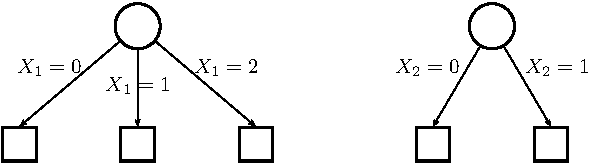
\includegraphics[scale=1.0]{figures/ch7_trees_id3.pdf}
    \caption{Totally randomized trees built from Table~\ref{table:simulation:bias:tree}. Both decision trees are equiprobable. The resulting variable importances indicate that both $X_1$ and $X_2$ are as important. }
    \label{fig:7:bias:trees:id3}
\end{figure}
\begin{figure}
    \centering
    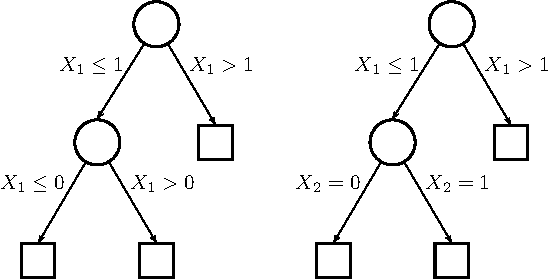
\includegraphics[scale=1.0]{figures/ch7_trees_ets.pdf}\vspace{1cm}\\
    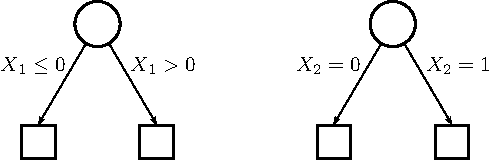
\includegraphics[scale=1.0]{figures/ch7_trees_ets2.pdf}
    \caption{Extremely randomized trees ($K=1$) built from Table~\ref{table:simulation:bias:tree}. From left to right, top to bottom, decision trees are respectively generated with probability $\tfrac{1}{8}$, $\tfrac{1}{8}$, $\tfrac{1}{4}$ and $\tfrac{1}{2}$. The resulting variable importances indicate that $X_2$ is now more important than $X_1$. }
    \label{fig:7:bias:trees:ets}
\end{figure}

By contrast, using binary splits and Extremely Randomized Trees (for $K=1$) results in $4$ different decision trees, as
represented in Figure~\ref{fig:7:bias:trees:ets}. When splitting on $X_1$ at
the root node, two binary splits are now possible with equal probability: $t_L = X_1 \leq 0, t_R = X_1 > 0$ or
$t_L = X_1 \leq 1, t_R = X_1 > 1$. In the former case, the resulting child nodes are pure,
hence halting the construction process. In the latter case, the right child
(corresponding to $X_1 > 1$) is pure, while the left child is not. For this
node, recursive partitioning proceeds and a second binary split can be made either on
$X_1$ or on $X_2$.  Overall, the measured variable
importances in these binary trees, in asymptotic conditions, are
\begin{align*}
\text{Imp}(X_1) &= \frac{2}{8} I(X_1 \leq 1;Y) + \frac{1}{8} P(X_1 \leq 1) I(X_1 \leq 0;Y|X_1 \leq 1) + \frac{1}{4} I(X_1 \leq 0;Y)\\
                &= 0.375 \\
\text{Imp}(X_2) &= \frac{1}{2} I(X_2;Y) + \frac{1}{8} P(X_1 \leq 1) I(X_2;Y|X_1\leq 1)\\
                &= 0.541,
\end{align*}
which makes them strictly different from the importances collected from multiway totally
randomized trees. In particular, due to the binarization of the split
variables, importances now account for conditioning sets that may include
several values of a same variable. For instance, the importance of $X_2$
includes $I(X_2;Y|X_1\leq 1)$, which measures the mutual information between
$X_2$ and $Y$ when $X_1$ is either equal to $0$ or $1$. With multiway
exhaustive splits, these conditioning sets are not considered because branches
correspond to single values only. Similarly, importances also account for
binarized mutual information terms such as $I(X_1 \leq 1;Y)$. Again, these are
not evaluated in totally randomized trees because of the multiway splits.

Accordingly, threshold selection in binary splits has a dominant effect on
variable importances since it controls how the original variables are
binarized. In ETs, all intermediate thresholds $v$ are possible, resulting in a
combinatorial number of additional impurity terms $I(X_j \leq v_j;Y|\cdot)$ and
$I(\cdot;Y|X_j \leq v_j, \cdot)$. In RF, only the best threshold is selected
locally at each node, resulting in fewer additional impurity terms $I(X_j <
v_j^*;Y|\cdot)$ and $I(\cdot;Y|X_j < v_j^*,\cdot)$ (and masking all others).

\begin{figure}
\centering
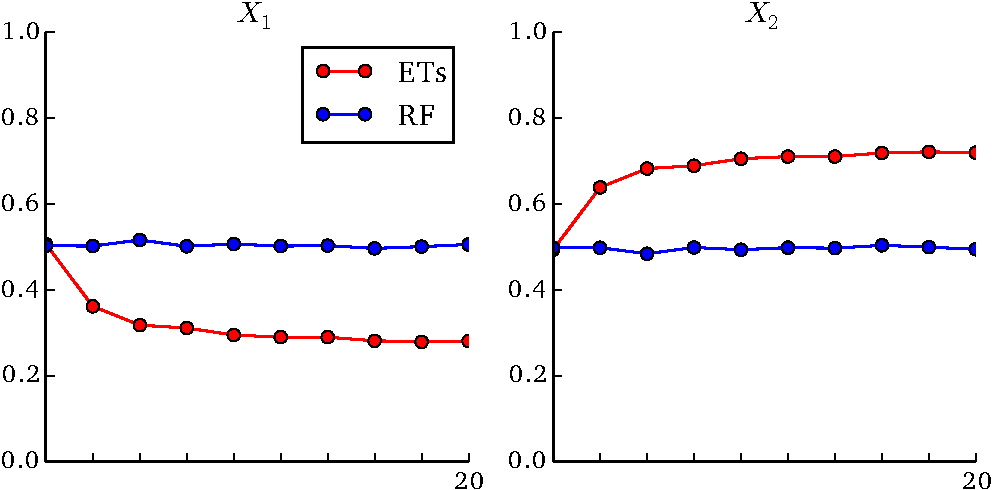
\includegraphics[width=0.9\textwidth]{figures/ch7_bias_trees.pdf}
\caption{Variable importances of $X_1$ and $X_2$ when increasing the cardinality of $X_1$. High cardinality does not necessarily mean high importance. }
\label{fig:7:bias:trees}
\end{figure}

As a last example, Figure~\ref{fig:7:bias:trees} illustrates variable
importances for $X_1$ and $X_2$ when increasing the cardinality of $X_1$ on the
previous toy problem. That is, let us redefine the output as $Y = X_1 <
\tfrac{|{\cal X}_1|}{2}$ while keeping $X_2$ as a binary variable defined as a
copy of $Y$. Assuming that all input samples are equiprobable, the importances
yielded by totally randomized trees with multiway splits remain the same as
before. For ETs however, increasing $|{\cal X}_1|$ induces even more new impurity terms
that are now accounted for in the importances. As the figure shows, increasing
the cardinality of $X_1$ makes its importance decrease, but also simultaneously
makes the importance of $X_2$ increase. Indeed, splitting on $X_2$ always yield
child nodes that are pure, which is unlikely to be the case when splitting
randomly on $X_1$. For RF, only the best thresholds are selected, yielding in
this case child nodes that are always pure, as for totally randomized trees.
As such, their importances respectively appear as equal as the figure confirms.

Overall, these additional effects due to binary splits make variable
importances computed from classical random forests very difficult to interpret
and understand, as soon as data include many variables of different scale
or number of categories. While they can still be
used to identify the most relevant variables, caution should be taken when
interpreting the amplitude of importance measures. As our last example
illustrates, the importance of a variable may be misleadingly low or
misleadingly high because of combinatorial effects, solely due to the possible
ways variables are binarized.

\begin{remark}{Encoding $N$-ary variables into binary variables}
Partitioning node samples with binary splits on $N$-ary input variables is
equivalent to individually transforming each input variable $X_j$ into a set of
$b_j$ binary input variables $\{X_j^{m} | m=1,\dots,b_j\}$, each encoding for
one the possible splits, and then partitioning node samples using of one these new
variables. If we consider the binarized learning set ${\cal L}^\prime$, for
which all $p$ the input variables have been transformed into $\sum b_j$ binary
variables, then our theoretical framework for totally randomized trees and
exhaustive splits can be applied and Theorem~\ref{thm:imp} could possibly be
adapted. The only difference lies in the way binary variables are drawn at
random:  instead of splitting randomly on one of the $\sum b_j$ variables,
first, one of the $p$ original variables is drawn uniformly at random; second, one of
its $b_j$ binary variables is selected for splitting the current node. In this
setting, the importance of $X_j$ therefore amounts to the sum of importances $\sum
\text{Imp}(X_j^m)$ of its binary variables. \end{remark}


\section{Applications}
\label{sec:7:applications}

In spite of the various concurrent effects discussed earlier, variable importance
measures have been used with success in a wide range of scientific
applications.  While  they have proven to be a good proxy for assessing the
relevance of input variables, providing helpful insights, too often variable
importances are used as a black-box metric, hence under-exploiting the
information they offer. As such, examples presented in this section all
demonstrate that any progress towards a better theoretical understanding of
variable importances may help to further advance a wide range of research
domains.

\subsection{Feature selection}

Within the past 10 or 20 years, typical machine learning problems have
grown from a few tens of input variables to domains exploring hundreds of
thousands of variables, often comprising noisy, irrelevant or redundant
predictors, mixing both numerical and categorical variables and involving
complex interaction effects. In this context, the feature selection problem
consists in identifying a subset of the original input variables that are
useful for building a good model~\citep{guyon:2003,liu:2005}. The
advantages and benefits of reducing the dimensionality of the problem
include: speeding up machine learning algorithms, reducing measurement and
storage requirements, improving the accuracy of the models or facilitating
data visualization and understanding.

Because of the properties of random forests (good prediction performance,
robustness to noisy variables, support of numerical and categorical
variables and ability to model complex interactions), variable importances
often provide an effective solution for the feature selection problem. The
most straightforward solution consists in ranking variables according to
their importance scores and to only keep the most important ones. Depending
on the objective, the best subset of variables can be identified in
several ways:

\begin{itemize}
\item  When the goal is simply to reduce dimensionality because of speed
       and storage requirements, the simplest solution
       is to keep only those variables whose importances $\text{Imp}(X_j)$
       is greater than some manually defined threshold $\alpha$.

\item If the goal is to improve accuracy, a good subset
      of variables can typically be found by tuning the threshold $\alpha$ so
      as to minimize some user-defined criterion (e.g., the zero-one loss in
      classification or the squared error loss in regression) for the model
      built on the subset $\{X_j | \text{Imp}(X_j) > \alpha \}$.

      At the price of more computational efforts, even better performance can
      usually be reached by embedding variable importances into a dedicated
      iterative feature selection procedure, such as those described in
      \citep{guyon:2002,tuv:2009}.

\item In some other applications, the objective is to identify variables
      that are relevant, in order to better understand the underlying relations
      with the output $Y$. In asymptotic conditions, this could be done by
      discarding all variables whose importances is null, as shown by
      Theorem~\ref{thm:relevant}. In a finite setting however, bias due to
      masking effects or impurity misestimations (as previously discussed in
      Section~\ref{sec:7:bias}) makes it more difficult to identify variables
      that are truly relevant since their importances might appear to be lower
      than those of irrelevant variables. Yet, several options are available
      for controlling and limiting false positives, such as stopping the
      construction process when impurity estimations become statistically
      unreliable (Section~\ref{sec:7:bias:high}), comparing the importances of
      the original input variables to artificial contrasts \citep{tuv:2006} or
      robustly controlling the conditional error rate through permutation tests
      \citep{saeys:2012}.

\end{itemize}


\subsection{Biomarker identification}

With the rise of \textit{-omics} data, random forests have become one of the
most popular tools in life sciences, providing practitioners with both
high-prediction accuracy and helpful insights about the importances of variables. In
many cases, variable importance measures (either MDI or the permutation
importance) is exploited to better understand the complex interaction effects
between the inputs and the output. Examples of successful applications include
the identification of risk-associated SNPs in genome-wide association studies
\citep{lunetta:2004,meng:2009,botta:2014}, the discovery of important genes and
pathways from micro-array gene-expression data \citep{pang:2006,chang:2008} or
the identification of factors for predicting protein-protein
interactions~\citep{qi:2006}. These examples are not isolated and tens of
further studies based on random forests could in fact be cited from the fields
of genomics, metabolomics, proteomics or transcriptomics. Some of them are
reviewed in \citep{touw:2013,boulesteix:2012}.

In light of our study and discussion of variable importances,  recommendations
for biomarker identification depend on the exact objective of the application.
If the goal is to identify all relevant variables, then totally randomized
trees with multiway splits should be prefered. They indeed constitute the only
method for which variable importances are unbiased, taking into account all
possible interaction terms in a fair and exhaustive way. The only caveat is
that a (very) large number of trees may be required before variable importances
converge, making them computationally intensive to compute, even if the full
randomization of the induction procedure actually make indidual decision trees
to be quite fast to generate.  By contrast, if the objective is only to
identify a subset of good predictors for predicting the output (hence possibly
omitting relevant but redundant variables), then non-totally randomized trees
(e.g., standard RF or ETs) with $K$ chosen to maximize accuracy should be
preferred. Even if some informative variables may be masked because of variable
selection, a good subset of input variables should still be identifiable from
importance scores. In all cases, impurity misestimations should be controlled
by stopping the construction process early or collecting importances only for
those nodes where impurity reductions can be considered as reliable. Whenever
practical, variable importances should also be decomposed in order to better
understand why some variables appear as more important than others. In
particular, studying the decomposition might help identify redundancy effects.

\subsection{Network inference}
\todo{}
%\citep{irrthum:2010}



\cleardoublepage
%\ctparttex{}
\part{Subsampling data}\label{part:3}
\chapter{Ensembles on Random Patches}\label{ch:random-patches}

% sampling samples: an easy way to reduce time complexity
% sampling features: an easy way to decorrelate predictions

\begin{remark}{Outline}
In this chapter, we consider supervised learning under the assumption that the
available memory is small compared to the size of the dataset. This general framework
is relevant in the context of big data, distributed databases and embedded
systems. In Section~\ref{sec:9:rp}, we propose a very simple, yet effective,
ensemble framework that builds each individual model of the ensemble from a
random patch of data obtained by drawing random subsets of \textit{both}
samples and input variables from the whole dataset. In
sections~\ref{sec:9:accuracy} and \ref{sec:9:memory}, we carry out an extensive
and systematic evaluation of this method on 29 datasets, using decision trees
as base models. With respect to popular ensemble methods, these experiments
show that the proposed method provides on par  performance  in terms of
accuracy while simultaneously lowering the memory needs, and attains
significantly better performance when memory is severely constrained. We
conclude and discuss future work directions in Section~\ref{sec:9:conclusions}.
\textit{This chapter is based on previous work published in \citep{louppe:2012}.}
\end{remark}

Within the past few years, big data has become a popular trend among many
scientific fields. In life sciences, computer vision, Internet search or
finance, to cite a few, quantities of data have grown so large that it is
increasingly difficult to process, analyze or visualize. In many cases, single
computers are no longer fit for big data and distributed environments need to
be considered to handle it. Although research is very active in this area,
machine learning is no exception to this new paradigm. Much still needs to be
done and methods and algorithms have to be reinvented to take this constraint
into account.

In this context, we consider supervised learning problems for which the dataset
is so large that it cannot be loaded into memory. \citet{breiman:1999} proposed
the Pasting method to tackle this problem by learning an ensemble of models
individually built on random subsets of the training examples, hence
alleviating the memory requirements since the base models would be built on
only small parts of the whole dataset. Earlier, \citet{ho:1998} proposed to
learn an ensemble of models individually built on random subspaces, i.e., on
random subsets of the input variables (or \textit{features}). While the first motivation of the Random
Subspace method was to increase the diversity within the models of the
ensemble, it can actually also be seen as way to reduce the memory requirements
of building individual models. In this work, we propose to combine and leverage
both approaches at the same time: learn an ensemble of models on \textit{random
patches}, i.e., on random subsets of the samples \textit{and} of the input
variables. Through an extensive empirical study, we show that this approach (1)
improves or preserves comparable accuracy with respect to other ensemble
approaches which build base models on the whole dataset while (2) drastically
lowering the memory requirements and hence allowing an equivalent reduction of
the global computing time. In other words, this analysis shows that there is
usually no need to build individual models on the whole dataset. For the same
accuracy, models can be learned independently on small portions of the data,
within significantly lower computational requirements.

\section{Random Patches}
\label{sec:9:rp}

The Random Patches algorithm proposed in this work (further referred to as RP)
is a wrapper ensemble method that can be described in the following terms. Let
${\cal R}(\alpha_s, \alpha_f, {\cal L})$ be the set of all random patches of
size $\alpha_s N \times \alpha_f p$ than can be drawn from the dataset ${\cal
L}$, where $N$ (resp., $p$) is the number of samples in ${\cal L}$ (resp.,  the
number of input variables in ${\cal L}$) and where $\alpha_s \in [0, 1]$\label{ntn:alpha_s} (resp.
$\alpha_f$\label{ntn:alpha_f}) is an hyper-parameter that controls the number of samples in a
patch (resp., the number of variables). That is, ${\cal R}(\alpha_s, \alpha_f,
{\cal L})$ is the set of all possible subsets containing $\alpha_s N$ samples
(among $N$) with $\alpha_f p$ variables (among $p$). The method then works as
follows:

\begin{algorithm}\label{algo:rp}
Random Patches algorithm.
\textnormal{
\begin{algorithmic}[1]
    \For{$m=1, \dots, M$}
        \State Draw a patch $r \sim U({\cal R}(\alpha_s, \alpha_f, {\cal L}))$ uniformly at random
        \State Build a model on the selected patch $r$
    \EndFor
    \State Aggregate the predictions of the $M$ models in an ensemble
\end{algorithmic}
}
\end{algorithm}

While the RP algorithm can exploit any kind of base estimators, we consider in
this work only tree-based estimators. In particular, we evaluate the RP
algorithm using  standard classification trees (as described in
Chapter~\ref{ch:cart}) and (single) extremely randomized
trees~\citep{geurts:2006}. Unless stated otherwise, trees are unpruned and
grown using Gini index as impurity criterion for node splitting. The
parameter $K$ of extremely randomized trees within RP is set to its maximum
value $K=\alpha_f p$ (i.e., corresponding to no further random selection of
variables).

The first benefit of RP is that it generalizes both the Pasting Rvotes (P)
method~\citep{breiman:1999} (and its extensions \citep{chawla:2004,basilico:2011})
and the Random Subspace (RS) algorithm~\citep{ho:1998}. Both are indeed merely
particular cases of RP: setting $\alpha_s=1.0$ yields RS while setting
$\alpha_f=1.0$ yields P. As such, it is expected that when both
hyper-parameters $\alpha_s$ and $\alpha_f$ are tuned simultaneously, RP should be at
least as good as the best of the two methods, provided there is no overfitting
associated with this tuning.

When the base estimators are standard decision trees (resp., extremely
randomized trees with $K=\alpha_f p$), interesting parallels can also be
drawn between RP and the RF algorithm (resp., ET). For $\alpha_s=1.0$, the
value of $\alpha_f p$ is indeed nearly equivalent to the number $K$ of
features randomly considered when splitting a node. A major difference
remains though. In RP, the subset of features is selected globally
once and for all, prior to the construction of each tree. By contrast,
in RF (resp., in ET) subsets of features are drawn locally at each
node. Clearly, the former approach already appears to be more
attractive when dealing with large databases. Non-selected features
indeed do not need to be considered at all, hence lowering the memory
requirements for building a single tree. Another interesting parallel
can be made when bootstrap samples are used like in RF: it nearly
amounts to set $\alpha_s=0.632$, i.e. the average proportion of unique
samples in a bootstrap sample. Differences are that in a bootstrap
sample, the number of unique training samples varies from one to
another (while it would be fixed to $0.632 N$ in RP), and that
samples are not all equally weighted.

In addition, RP also closely relates to the SubBag algorithm
which combines Bagging and RS for constructing ensembles. Using $N$
bootstrapped samples (i.e., nearly equivalent to $\alpha_s=0.632$) and setting
$\alpha_f=0.75$, \citet{panov:2007} showed that SubBag has comparable performance to that of
RF. An added advantage of SubBag, and hence of RP, is that it is applicable to
any base estimator without the need to randomize the latter.


\section{On Accuracy}
\label{sec:9:accuracy}

Our validation of the RP algorithm is carried out in two
steps. In this section, we first investigate how RP compares with
other popular tree-based ensemble methods in terms of accuracy. In the
next section, we then focus on its memory requirements for
achieving optimal accuracy and its capability to handle strong memory
constraints, again in comparison with other ensemble methods.

Considering accuracy only, our main objective is to investigate whether the
additional degrees of freedom brought by $\alpha_s$ and $\alpha_f$ significantly improve,
or degrade, the performance of RP. At first glance, one might indeed think that
since the base estimators are (intentionally) built on parts of the data, the
accuracy of the ensemble will be lower than if they were all built on the whole
set. Additionally, our goal is also to see whether sampling features once
globally, instead of locally at each node, impairs performance, as this is the
main difference between RP and state-of-the-art methods such as RF or ET.

\subsection{Protocol}

We compare our method with P and RS, as well as with RF and ET. For RP, P and
RS, two variants have been considered, one using standard decision trees
(suffixed below with '-DT') as base estimators, and the other using extremely
randomized trees (suffixed below with '-ET') as base estimators.  Overall, 8
methods are compared: RP-DT, RP-ET, P-DT, P-ET, RS-DT, RS-ET, RF and ET.

We evaluate the accuracy of the methods on an extensive list of both
artificial and real classification problems.  For each dataset, three
random partitions were drawn: the first and larger (50\% of the
original dataset) to be used as the training set, the second (25\%) as
validation set and the third (25\%) as test set. For all methods, the
hyper-parameters $\alpha_s$ and $\alpha_f$ were tuned on the validation set with
a grid-search procedure, using the grid \{0.01, 0.1, ..., 0.9, 1.0\}
for both $\alpha_s$ and $\alpha_f$. All other hyper-parameters were set to
default values. In RF and ET, the number $K$ of features randomly
selected at each node was tuned using the grid $\alpha_f p$. For all
ensembles, 250 fully developed trees were generated and the
generalization accuracy was estimated on the test set. Unless
otherwise mentioned, for all methods and for all datasets, that
procedure was repeated 50 times, using the same 50 random partitions
between all methods, and all scores reported below are averages over
those 50 runs. All algorithms and experiments have been implemented in
Python, using Scikit-Learn~\citep{pedregosa:2011} as base framework.

\subsection{Small datasets}

Before diving into heavily computational experiments, we first wanted to
validate our approach on small to medium datasets. To that end, experiments
were carried out on a sample of 16 well-known and publicly
available datasets (see Table~\ref{table:rp:small-data}) from the UCI machine
learning repository~\citep{frank:2010}, all chosen a priori and
independently of the results obtained. Overall, these datasets cover a wide
range of conditions, with the sample sizes ranging from 208 to 20000 and the
number of features varying from 6 to 168. Detailed average performances of the
8 methods for all 16 datasets using the protocol described above are reported
in Table~\ref{table:rp:accuracy}. Below, we analyze general trends by performing
various statistical tests.

\begin{table}
    \centering
    \footnotesize
    \begin{tabular}{| l | c c |}
    \hline
    \textbf{Dataset} & $N$ & $p$ \\
    \hline
    \hline
        \textsc{diabetes}    & 768       & 8         \\
        \textsc{dig44}       & 18000     & 16        \\
        \textsc{ionosphere}  & 351       & 34        \\
        \textsc{pendigits}   & 10992     & 16        \\
        \textsc{letter}      & 20000     & 16        \\
        \textsc{liver}       & 345       & 6         \\
        \textsc{musk2}       & 6598      & 168       \\
        \textsc{ring-norm}   & 10000     & 20        \\
        \textsc{satellite}   & 6435      & 36        \\
        \textsc{segment}     & 2310      & 19        \\
        \textsc{sonar}       & 208       & 60        \\
        \textsc{spambase}    & 4601      & 57        \\
        \textsc{two-norm}    & 9999      & 20        \\
        \textsc{vehicle}     & 1692      & 18        \\
        \textsc{vowel}       & 990       & 10        \\
        \textsc{waveform}    & 5000      & 21        \\
    \hline
    \end{tabular}
    \caption{Small datasets.}
    \label{table:rp:small-data}
\end{table}

\begin{table}
    \centering
    \footnotesize
    \hspace{-3.2cm}
\begin{tabular}{|l|cccccccc|}
\hline
\textbf{Validation} & RF & ET & P-DT & P-ET & RS-DT & RS-ET & RP-DT & RP-ET \\
\hline
\hline
    \textsc{diabetes  }  & 77.12 (6)    & 77.25 (5)    & 77.67 (4)    & 78.01 (3)    & 75.11 (8)    & 76.77 (7)    & 78.82 (2)   &  \textbf{79.07} (1) \\
    \textsc{dig44     }  & 94.99 (7)    & \textbf{95.78} (1)    & 91.86 (8)    & 95.46 (4)    & 95.07 (6)    & 95.69 (3)    & 95.13 (5)   &  95.72 (2) \\
    \textsc{ionosphere}  & 94.40 (6)    & 95.15 (3)    & 93.86 (8)    & 94.75 (5)    & 94.11 (7)    & 94.90 (4)    & 95.20 (2)   &  \textbf{95.36} (1) \\
    \textsc{pendigits }  & 98.94 (7)    & \textbf{99.33} (1)    & 98.09 (8)    & 99.28 (4)    & 99.02 (6)    & 99.31 (3)    & 99.07 (5)   &  99.32 (2) \\
    \textsc{letter    }  & 95.36 (7)    & \textbf{96.38} (1)    & 92.72 (8)    & 95.87 (4)    & 95.68 (6)    & 96.08 (3)    & 95.74 (5)   &  96.10 (2) \\
    \textsc{liver     }  & 72.37 (5)    & 71.90 (6)    & 72.55 (4)    & 72.88 (3)    & 68.06 (8)    & 70.88 (7)    & \textbf{74.53} (1)   &  74.37 (2) \\
    \textsc{musk2     }  & 97.18 (7)    & \textbf{97.73} (1)    & 96.89 (8)    & 97.60 (4)    & 97.58 (6)    & 97.72 (3)    & 97.60 (5)   &  97.73 (2) \\
    \textsc{ring-norm }  & 97.44 (6)    & 98.10 (5)    & 96.41 (8)    & 97.28 (7)    & 98.25 (4)    & 98.41 (3)    & 98.50 (2)   &  \textbf{98.54} (1) \\
    \textsc{satellite }  & 90.97 (7)    & \textbf{91.56} (1)    & 90.01 (8)    & 91.40 (5)    & 91.31 (6)    & 91.50 (3)    & 91.41 (4)   &  91.54 (2) \\
    \textsc{segment   }  & 97.46 (6)    & 98.17 (2)    & 96.78 (8)    & 98.10 (4)    & 97.33 (7)    & 98.14 (3)    & 97.52 (5)   &  \textbf{98.21} (1) \\
    \textsc{sonar     }  & 82.92 (7)    & 86.92 (3)    & 80.03 (8)    & 84.73 (5)    & 83.07 (6)    & 87.07 (2)    & 85.42 (4)   &  \textbf{88.15} (1) \\
    \textsc{spambase  }  & 94.80 (7)    & 95.36 (3)    & 93.69 (8)    & 95.01 (6)    & 95.01 (5)    & 95.50 (2)    & 95.11 (4)   &  \textbf{95.57} (1) \\
    \textsc{two-norm  }  & 97.54 (6)    & 97.77 (2)    & 97.52 (7)    & 97.59 (5)    & 97.46 (8)    & 97.63 (4)    & 97.76 (3)   &  \textbf{97.82} (1) \\
    \textsc{vehicle   }  & 88.67 (5)    & 88.68 (4)    & 88.26 (8)    & 88.74 (3)    & 88.41 (7)    & 88.60 (6)    & \textbf{89.22} (1)   &  89.21 (2) \\
    \textsc{vowel     }  & 92.04 (5)    & \textbf{95.12} (1)    & 85.19 (8)    & 93.49 (4)    & 89.76 (7)    & 94.34 (3)    & 91.10 (6)   &  94.48 (2) \\
    \textsc{waveform  }  & 85.45 (6)    & 85.96 (2)    & 84.89 (8)    & 85.68 (5)    & 84.91 (7)    & 85.69 (4)    & 85.85 (3)   &  \textbf{86.21} (1) \\
\hline
\textit{Average rank} & 6.25 & 2.5625 & 7.4375 & 4.4375 & 6.5 & 3.75 & 3.5626 & 1.5 \\
\hline
\hline
\textbf{Test} & RF & ET & P-DT & P-ET & RS-DT & RS-ET & RP-DT & RP-ET \\
\hline
\hline
    \textsc{diabetes  }  & 75.62 (4)    & 75.38 (5)    & 75.67 (3)    & \textbf{76.34} (1)    & 73.03 (8)    & 74.63 (7)    & 75.32 (6)   &  75.82 (2) \\
    \textsc{dig44     }  & 94.96 (6)    & \textbf{95.67} (1)    & 91.79 (8)    & 95.39 (4)    & 94.98 (5)    & 95.58 (2)    & 94.95 (7)   &  95.55 (3) \\
    \textsc{ionosphere}  & 92.20 (6)    & \textbf{93.22} (1)    & 92.09 (7)    & 92.40 (4)    & 92.02 (8)    & 93.22 (2)    & 92.34 (5)   &  92.68 (3) \\
    \textsc{pendigits }  & 98.84 (7)    & \textbf{99.23} (1)    & 97.97 (8)    & 99.21 (3)    & 98.95 (5)    & 99.21 (2)    & 98.93 (6)   &  99.20 (4) \\
    \textsc{letter    }  & 95.27 (7)    & \textbf{96.29} (1)    & 92.57 (8)    & 95.89 (4)    & 95.61 (5)    & 96.03 (2)    & 95.61 (6)   &  95.99 (3) \\
    \textsc{liver     }  & 69.95 (3)    & 68.22 (6)    & \textbf{70.43} (1)    & 69.58 (5)    & 63.17 (8)    & 67.35 (7)    & 70.20 (2)   &  69.67 (4) \\
    \textsc{musk2     }  & 97.08 (7)    & \textbf{97.61} (1)    & 96.69 (8)    & 97.54 (4)    & 97.47 (5)    & 97.58 (2)    & 97.42 (6)   &  97.56 (3) \\
    \textsc{ring-norm }  & 97.48 (6)    & 98.07 (5)    & 96.42 (8)    & 97.25 (7)    & 98.16 (4)    & \textbf{98.31} (1)    & 98.22 (3)   &  98.30 (2) \\
    \textsc{satellite }  & 90.67 (7)    & 91.22 (2)    & 89.66 (8)    & 91.20 (3)    & 91.15 (5)    & \textbf{91.28} (1)    & 91.04 (6)   &  91.20 (4) \\
    \textsc{segment   }  & 97.02 (5)    & \textbf{97.93} (1)    & 96.44 (8)    & 97.86 (3)    & 96.86 (7)    & 97.90 (2)    & 96.88 (6)   &  97.84 (4) \\
    \textsc{sonar     }  & 79.53 (5)    & \textbf{82.76} (1)    & 75.15 (8)    & 80.07 (4)    & 78.50 (6)    & 82.19 (2)    & 78.26 (7)   &  81.92 (3) \\
    \textsc{spambase  }  & 94.76 (7)    & 95.17 (3)    & 93.51 (8)    & 94.84 (5)    & 94.88 (4)    & 95.22 (2)    & 94.80 (6)   &  \textbf{95.22} (1) \\
    \textsc{two-norm  }  & 97.22 (7)    & \textbf{97.50} (1)    & 97.26 (6)    & 97.29 (4)    & 97.20 (8)    & 97.33 (2)    & 97.33 (3)   &  97.28 (5) \\
    \textsc{vehicle   }  & 87.47 (7)    & 87.85 (3)    & 87.01 (8)    & 87.98 (2)    & 87.50 (6)    & 87.68 (5)    & 87.73 (4)   &  \textbf{88.08} (1) \\
    \textsc{vowel     }  & 91.51 (5)    & \textbf{93.95} (1)    & 84.17 (8)    & 92.93 (4)    & 89.51 (7)    & 93.60 (2)    & 89.89 (6)   &  93.09 (3) \\
    \textsc{waveform  }  & 85.23 (5)    & \textbf{85.77} (1)    & 84.68 (8)    & 85.40 (3)    & 84.74 (7)    & 85.38 (4)    & 85.16 (6)   &  85.56 (2) \\
\hline
\textit{Average rank} & 5.875 & 2.125 & 7.0625 & 3.75 & 6.125 & 2.8125 & 5.3125 & 2.9375 \\
\hline
\end{tabular}
    \caption{Accuracy on small datasets (in \%).}
    \label{table:rp:accuracy}
\end{table}

Following recommendations in \citep{demsar:2006}, we first performed a
Friedman test that rejected the hypothesis that all algorithms are
equivalent at a significance level $\alpha=0.05$.
We then proceeded with a post-hoc Nemenyi test for a
pairwise comparison of the average ranks of all 8 methods. According to
this test, the performance of two classifiers is significantly
different (at $\alpha=0.05$) if their average ranks differ by at least
the critical difference $CD = 2.6249$
(See~\citep{demsar:2006} for further details). The diagram of
Figure~\ref{fig:8:small-cmp} summarizes these comparisons. The top line
in the diagram is the axis along which the average rank $R_m$ of each method $m$ is plotted,
from the highest ranks (worst methods) on the left to the lowest ranks
(best methods) on the right.  Groups of methods that are not
statistically different from each other are connected. The critical
difference CD is shown above the graph.  To further support these rank
comparisons, we also compare the 50 accuracy values obtained
over each dataset split for each pair of methods by using a paired
t-test (with $\alpha=0.01$). The results of these comparisons are
summarized in Table \ref{table:rp:small-ttest} in terms of ``Win-Draw-Loss''
statuses of all pairs of methods; the three values at the intersection
of row $i$ and column $j$ of this table respectively indicate on how
many datasets method $i$ is significantly better/not significantly
different/significantly worse than method $j$.

\begin{figure}
    \centering
    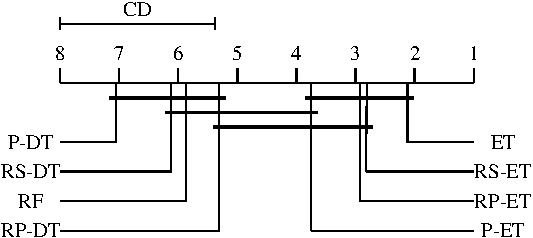
\includegraphics[width=0.9\textwidth]{figures/ch8_rank_small.pdf}
    \caption{Average ranks of all methods on small datasets.}
    \label{fig:8:small-cmp}
\end{figure}

\begin{table}
    \centering
    \footnotesize
  \begin{tabular}{|l|cccccccc|}
    \hline
         & RF & ET & P-DT & P-ET & RS-DT & RS-ET & RP-DT & RP-ET \\
    \hline
    \hline
        RF     &  ---   & 1/2/13 & 12/4/0  & 1/7/8   & 4/7/5   & 2/2/12 & 1/10/5  & 0/4/12 \\
        ET     &  13/2/1 & ---   & 14/1/1  & 10/5/1  & 13/3/0  & 4/11/1 & 12/2/2  & 5/10/1 \\
        P-DT   &  0/4/12 & 1/1/14 & ---    & 0/4/12  & 2/3/11  & 2/1/13 & 0/4/12  & 0/4/12 \\
        P-ET   &  8/7/1  & 1/5/10 & 12/4/0  & ---    & 9/6/1   & 2/6/8  & 9/6/1   & 0/11/5 \\
        RS-DT  &  5/7/4  & 0/3/13 & 11/3/2  & 1/6/9   & ---    & 0/2/14 & 1/11/4  & 0/4/12 \\
        RS-ET  &  12/2/2 & 1/11/4 & 13/1/2  & 8/6/2   & 14/2/0  & ---   & 11/4/1  & 1/13/2 \\
        RP-DT  &  5/10/1 & 2/2/12 & 12/4/0  & 1/6/9   & 4/11/1  & 1/4/11 & ---    & 0/6/10 \\
        RP-ET  &  12/4/0 & 1/10/5 & 12/4/0  & 5/11/0  & 12/4/0  & 2/13/1 & 10/6/0  & ---\\
    \hline
    \end{tabular}
    \caption{Pairwise t-test comparisons on small datasets.}
    \label{table:rp:small-ttest}
\end{table}

% ET versus DT

Since all methods are variants of ensembles of decision trees, average
accuracies are not strikingly different from one method to another (see Table 1
of the supplementary materials). Yet, significant trends appear when looking at
Figure \ref{fig:8:small-cmp} and Table \ref{table:rp:small-ttest}.  First, all ET-based
methods are ranked before DT-based methods, including the popular Random
Forest algorithm. Overall, the original ET algorithm is ranked first ($R_{ET} =
2.125$), then come RS-ET and RP-ET at close positions ($R_{RS-ET} = 2.8125$ and
$R_{RP-ET} = 2.9375$) while P-ET is a bit behind ($R_{P-ET} = 3.75$). According
to Figure \ref{fig:8:small-cmp}, only ET is ranked significantly higher than all
DT-based method but looking at Table \ref{table:rp:small-ttest}, the worse ET-based
variant (P-ET) is still 9 times significantly better (w.r.t. the 50
runs over each set) and only 1 times significantly worse than the best DT-based
variant (RP-DT). The separation between these two families of algorithm
thus appears quite significant. This observation clearly suggests that using
random split thresholds, instead of optimized ones like in decision trees, pays
off in terms of generalization.

% RP versus RS et P (ET)

Among ET-based methods, RP-ET is better than P-ET but it is superseded by ET and
RS-ET in terms of average rank. Since RS-ET is a particular case of RP-ET, this
suggests that we are slightly overfitting when tuning the additional parameter
$\alpha_s$. And indeed RP-ET is better ranked than RS-ET in average on the validation
set (results not shown). Table~\ref{table:rp:small-ttest} however indicates
otherwise and makes RP-ET appear as slightly better than RS-ET (2/13/1).
Regarding ET over RP-ET, the better performance of the former (5/10/1) is
probably due to the fact that in ET subsets of features are redrawn locally at
each node when building trees and not once and for all prior to their
construction. This gives less chances to generate improper trees because of a
bad initial choice of features and thus leads to a lower bias and a better
accuracy.

% RP versus RS et P (DT)

Among DT-based methods, RP-DT now comes first (mean rank of 5.3125),
then RF ($R_{RF} = 5.875$), RS-DT ($R_{RS-DT} = 6.125$) and then P-DT
in last ($R_{P-DT} = 7.0625$). RP is only significantly worse than
another DT-based variant on 1 dataset. The extra-randomization brought
by the random choices of both samples and features seems to be
beneficial with decision trees that do not benefit from the
randomization of discretization thresholds. The fact that RF samples
features locally does not appear here anymore as an advantage over RP
(RF is significantly worse on 5 problems and better on only one),
probably because the decrease of bias that it provides does not exceed
the increase of variance with respect to global feature selection.

\subsection{Larger datasets}

While the former experiments revealed promising results, it is fair to ask
whether the conclusions that have been drawn would hold on and generalize to
larger problems, for example when dealing with a few relevant features buried
into hundreds or thousands of not important features (e.g., in genomic data),
or when dealing with many correlated features (e.g., in images). To investigate
this question, a second bench of experiments was carried out on 13 larger
datasets (see Table~\ref{table:rp:large-data}). All but
\textsc{madelon} are real data. In terms of dimensions, these datasets are far bigger,
ranging from a few hundreds of samples and thousands of features, to thousands of
samples but hundreds of features. As such, the complexity of the problems is
expected to be greater.  We adopted the exact same protocol as for smaller
datasets. However, to lower computing times, for datasets marked with $*$, the
methods were run using 100 trees instead of 250 and the minimum number of
samples required in an internal node was set to 10 in order to control
complexity. Detailed results are provided in Table~\ref{table:rp:accuracy-large}
and are summarized in Figure \ref{fig:8:large-cmp} and
Table \ref{table:rp:large-ttest}, respectively in terms of average rank (the
critical difference at $\alpha=0.05$ is now 2.9120) and Win/Draw/Loss statuses
obtained with paired t-tests. A Friedman test (at $\alpha=0.05$) still
indicates that some methods are significantly different from the others.

\begin{table}
    \centering
    \footnotesize
    \begin{tabular}{| l | c c |}
    \hline
    \textbf{Dataset} & $N$ & $p$ \\
    \hline
    \hline
                \textsc{cifar10}*   & 60000   & 3072   \\
                \textsc{mnist3vs8}  & 13966   & 784    \\
                \textsc{mnist4vs9}  & 13782   & 784    \\
                \textsc{mnist}*     & 70000   & 784    \\
                \textsc{isolet}     & 7797    & 617    \\
                \textsc{arcene}     & 900     & 10000  \\
                \textsc{breast2}    & 295     & 24496  \\
                \textsc{madelon}    & 4400    & 500    \\
                \textsc{marti0}     & 500     & 1024   \\
                \textsc{reged0}     & 500     & 999    \\
                \textsc{secom}      & 1567    & 591    \\
                \textsc{tis}        & 13375   & 927    \\
                \textsc{sido0}*     & 12678   & 4932   \\
    \hline
    \end{tabular}
    \caption{Large datasets.}
    \label{table:rp:large-data}
\end{table}

\begin{table}
    \centering
    \footnotesize
    \hspace{-3.2cm}
\begin{tabular}{|l|cccccccc|}
\hline
\textbf{Validation} & RF & ET & P-DT & P-ET & RS-DT & RS-ET & RP-DT & RP-ET \\
\hline
\hline
    \textsc{cifar10 }  &  45.16 (6)  &  \textbf{46.17} (1)  &  44.92 (7)  &  44.88 (8)  &  45.83 (5)  &  46.09 (3)  &  45.89 (4)  &  46.13 (2) \\
    \textsc{mnist3v8}  &  98.42 (7)  &  98.77 (5)  &  97.63 (8)  &  98.57 (6)  &  98.79 (4)  &  98.86 (2)  &  98.81 (3)  &  \textbf{98.87} (1) \\
    \textsc{mnist4v9}  &  98.47 (7)  &  98.82 (3)  &  97.39 (8)  &  98.47 (6)  &  98.77 (5)  &  98.89 (2)  &  98.80 (4)  &  \textbf{98.91} (1) \\
    \textsc{mnist   }  &  96.14 (7)  &  96.56 (3)  &  94.35 (8)  &  96.19 (6)  &  96.52 (5)  &  96.57 (2)  &  96.53 (4)  &  \textbf{96.57} (1) \\
    \textsc{isolet  }  &  93.96 (7)  &  95.07 (3)  &  90.90 (8)  &  94.23 (6)  &  94.38 (5)  &  95.15 (2)  &  94.47 (4)  &  \textbf{95.20} (1) \\
    \textsc{arcene  }  &  73.84 (7)  &  77.76 (3)  &  73.76 (8)  &  75.12 (6)  &  76.40 (5)  &  77.60 (4)  &  79.44 (2)  &  \textbf{80.00} (1) \\
    \textsc{breast2 }  &  69.64 (6)  &  69.91 (4)  &  70.54 (3)  &  69.83 (5)  &  69.59 (7)  &  69.54 (8)  &  \textbf{72.59} (1)  &  71.62 (2) \\
    \textsc{madelon }  &  76.12 (8)  &  \textbf{81.41} (1)  &  78.48 (7)  &  81.06 (5)  &  80.68 (6)  &  81.29 (3)  &  81.18 (4)  &  81.36 (2) \\
    \textsc{marti   }  &  87.66 (8)  &  87.92 (6)  &  88.08 (4)  &  88.09 (3)  &  87.77 (7)  &  88.00 (5)  &  88.19 (2)  &  \textbf{88.20} (1) \\
    \textsc{reged   }  &  98.00 (6)  &  98.46 (2)  &  97.08 (8)  &  98.24 (5)  &  98.00 (7)  &  98.41 (3)  &  98.40 (4)  &  \textbf{98.57} (1) \\
    \textsc{secom   }  &  93.37 (5)  &  93.36 (6)  &  93.34 (8)  &  93.42 (2)  &  93.35 (7)  &  93.40 (4)  &  93.41 (3)  &  \textbf{93.45} (1) \\
    \textsc{tis     }  &  91.81 (5)  &  91.53 (7)  &  91.59 (6)  &  91.50 (8)  &  92.04 (3)  &  91.97 (4)  &  \textbf{92.26} (1)  &  92.06 (2) \\
    \textsc{sido    }  &  97.46 (5)  &  97.44 (6)  &  97.36 (8)  &  97.36 (7)  &  97.47 (3)  &  97.46 (4)  &  \textbf{97.52} (1)  &  97.52 (2) \\
\hline
\textit{Avg. rank} & 6.4615 & 3.8461 & 7.0   & 5.6153 & 5.3076 & 3.5384 &  2.8461 & 1.3846 \\
\hline
\hline
\textbf{Test} & RF & ET & P-DT & P-ET & RS-DT & RS-ET & RP-DT & RP-ET \\
\hline
\hline
    \textsc{cifar10 }  &  44.87 (7)  &  45.95 (2)  &  44.75 (8)  &  44.95 (6)  &  45.86 (4)  &  \textbf{46.02} (1)  &  45.74 (5)  &  45.93 (3) \\
    \textsc{mnist3v8}  &  98.31 (7)  &  98.64 (5)  &  97.47 (8)  &  98.48 (6)  &  98.70 (2)  &  \textbf{98.71} (1)  &  98.68 (4)  &  98.68 (3) \\
    \textsc{mnist4v9}  &  98.33 (6)  &  98.68 (2)  &  97.16 (8)  &  98.32 (7)  &  98.59 (4)  &  \textbf{98.69} (1)  &  98.59 (5)  &  98.67 (3) \\
    \textsc{mnist   }  &  96.10 (7)  &  96.47 (3)  &  94.30 (8)  &  96.18 (6)  &  96.47 (4)  &  \textbf{96.49} (1)  &  96.46 (5)  &  96.48 (2) \\
    \textsc{isolet  }  &  93.87 (7)  &  \textbf{94.95} (1)  &  90.71 (8)  &  94.15 (6)  &  94.33 (4)  &  94.94 (2)  &  94.29 (5)  &  94.88 (3) \\
    \textsc{arcene  }  &  71.04 (4)  &  \textbf{72.56} (1)  &  66.16 (8)  &  68.56 (7)  &  71.52 (3)  &  72.24 (2)  &  69.44 (6)  &  70.00 (5) \\
    \textsc{breast2 }  &  65.86 (6)  &  \textbf{66.16} (1)  &  65.54 (8)  &  65.59 (7)  &  66.13 (2)  &  65.91 (5)  &  65.94 (4)  &  66.08 (3) \\
    \textsc{madelon }  &  75.33 (8)  &  \textbf{80.83} (1)  &  77.86 (7)  &  80.78 (2)  &  80.06 (6)  &  80.59 (3)  &  80.06 (5)  &  80.42 (4) \\
    \textsc{marti   }  &  87.74 (8)  &  87.85 (6)  &  \textbf{88.24} (1)  &  88.17 (2)  &  87.82 (7)  &  88.06 (4)  &  88.08 (3)  &  88.01 (5) \\
    \textsc{reged   }  &  97.60 (5)  &  \textbf{98.20} (1)  &  96.40 (8)  &  97.92 (3)  &  97.39 (6)  &  98.00 (2)  &  97.32 (7)  &  97.82 (4) \\
    \textsc{secom   }  &  93.30 (7)  &  93.22 (8)  &  \textbf{93.38} (1)  &  93.30 (6)  &  93.37 (2)  &  93.31 (4)  &  93.33 (3)  &  93.31 (5) \\
    \textsc{tis     }  &  91.68 (5)  &  91.42 (7)  &  91.49 (6)  &  91.40 (8)  &  \textbf{92.05} (1)  &  91.91 (3)  &  92.05 (2)  &  91.90 (4) \\
    \textsc{sido    }  &  97.33 (4)  &  97.33 (3)  &  97.26 (7)  &  97.26 (8)  &  \textbf{97.35} (1)  &  97.34 (2)  &  97.33 (5)  &  97.32 (6) \\
\hline
\textit{Avg. rank} & 6.2307 & 3.1538 & 6.6153 & 5.6923 & 3.5384 & 2.3846 & 4.5384 & 3.8461 \\
\hline
\end{tabular}
    \caption{Accuracy on larger datasets (in \%).}
    \label{table:rp:accuracy-large}
\end{table}

As it may be observed from Figure~\ref{fig:8:large-cmp}, the average ranks of the
methods are closer to each other than in the previous experiments, now ranging
from 2.38 to 6.61, while they were previously ranging from 2.12 to 7. Methods
are more connected by critical difference bars. This suggests that overall they
behave more similarly to each other than before. General trends are nevertheless
comparable to what we observed earlier. ET-based methods still seem to be the
front-runners.  From Figure~\ref{fig:8:large-cmp}, RS-ET, ET and RP-ET are in the
top 4, while P-DT, RF and RP-DT remain in the second half of the ranking.
Surprisingly however, RS-DT now comes right after RS-ET and ET and just before
RP-ET whereas it ranked penultimate on the smaller datasets. Table~\ref{table:rp:large-ttest}
however suggests that RS-DT performs actually a little worse
against RP-ET (1/10/2).  All in all, it thus still seems beneficial to randomize
split thresholds on the larger datasets.

Comparing ET-based variants, ET is no longer the best method on average, but RS-ET
is (with 4/9/0 for RS-ET versus ET). This suggests than on larger datasets,
picking features globally at random prior to the construction of the trees is as
good, or even beat picking them locally at each node. Due to the quantitatively
larger number of samples in a patch, and also to the larger number of redundant
features expected in some large datasets (e.g., in \textsc{cifar10} or \textsc{mnist}), it is
indeed less likely to build improper trees with strong biases. As a result,
variance can be further decreased by sampling globally. In support of this
claim, on a few problems such as \textsc{arcene}, \textsc{breast2}, or \textsc{madelon} that contain many
irrelevant features, ET remains the best method. In that case, it is indeed more
likely to sample globally improper random patches, and hence to build improper
trees. The average rank of RP-ET suggests that it performs worse than RS-ET and
thus that there is some potential overfitting when tuning $\alpha_s$ in addition to
$\alpha_f$. This difference is however not confirmed in Table~\ref{table:rp:large-ttest}
where the accuracies of these two methods are shown to be never significantly
different (0/13/0). RP-ET is also on a perfect par with ET (1/11/1). Among DT-based variants,
RP-DT, which was the best performer on small datasets, is still
ranked above RF and P-DT, but it is now ranked below RS-DT with a win/draw/loss
of 0/11/2. This is again due to some overfitting.

While less conclusive than before, the results on larger datasets are
consistent with what we observed earlier. In particular, they indicate that
the Random Patches method (with ET) remains competitive with the best
performers.

\begin{figure}
    \centering
    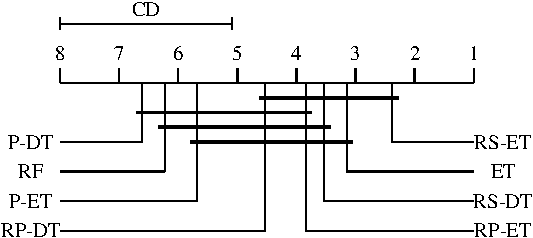
\includegraphics[width=0.9\textwidth]{figures/ch8_rank_large.pdf}
    \caption{Average ranks of all methods on larger datasets.}
    \label{fig:8:large-cmp}
\end{figure}

\begin{table}
    \centering
    \footnotesize
  \begin{tabular}{|l|cccccccc|}
    \hline
         & RF & ET & P-DT & P-ET & RS-DT & RS-ET & RP-DT & RP-ET \\
    \hline
    \hline
                RF     & ---    & 1/5/7   & 8/3/2  & 2/6/5  & 0/6/7  & 0/5/8  & 0/6/7  & 0/6/7 \\
                ET     & 7/5/1   & ---    & 9/2/2  & 7/6/0  & 3/7/3  & 0/9/4  & 5/6/2  & 1/11/1 \\
                P-DT   & 2/3/8   & 2/2/9   & ---   & 1/5/7  & 0/3/10 & 0/3/10 & 1/3/9  & 0/4/9 \\
                P-ET   & 5/6/2   & 0/6/7   & 7/5/1  & ---   & 0/6/7  & 0/5/8  & 2/5/6  & 1/5/7 \\
                RS-DT  & 7/6/0   & 3/7/3   & 10/3/0 & 7/6/0  & ---   & 1/8/4  & 2/11/0 & 1/10/2 \\
                RS-ET  & 8/5/0   & 4/9/0   & 10/3/0 & 8/5/0  & 4/8/1  & ---   & 4/8/1  & 0/13/0 \\
                RP-DT  & 7/6/0   & 2/6/5   & 9/3/1  & 6/5/2  & 0/11/2 & 1/8/4  & ---   & 1/9/3 \\
                RP-ET  & 7/6/0   & 1/11/1  & 9/4/0  & 7/5/1  & 2/10/1 & 0/13/0 & 3/9/1  & ---\\
    \hline
    \end{tabular}
    \caption{Pairwise t-test comparisons on larger datasets.}
    \label{table:rp:large-ttest}
\end{table}

\subsection{Conclusions}

Overall, this extensive experimental study reveals many interesting results. The
first and foremost result is that ensembles of randomized trees nearly always
beat ensembles of standard decision trees. As off-the-shelf methods, we advocate
that ensembles of such trees should be preferred to ensembles of decision trees.
In particular, these results show that the well-known Random Forest algorithm
does not compete with the best performers.  Far more important to our concern
though, this study validates our RP approach. Building ensembles (of ET) on
random patches of data is competitive in terms of accuracy. Overall, there is no
strong statistical evidence that the method performs less well, but there is
also no conclusive evidence that it significantly improves performance. Yet,
results show that RP is often as good as the very best methods. Regarding the
shape of the random patches, the strategy behind Pasting (i.e., $\alpha_s$ free and
$\alpha_f=1.0$) proved to be (very) ineffective on many datasets while the Random
Subspace algorithm (i.e., $\alpha_s=1.0$ and $\alpha_f$ free) always ranked among the very
best performers. On average, RS indeed came in second on the small datasets and
in first on the larger datasets, which tends to indicate that sampling features
is crucial in terms of accuracy. As for patches of freely adjustable size (i.e.,
using RP), they showed to be slightly sensitive to overfitting but proved to
remain closely competitive with the very best methods. In addition, these
results also suggest that sampling features globally, once and for all, prior to
the construction of a (randomized) decision tree, does not actually impair
performance. For instance, RS-ET or RP-ET are indeed not strongly worse, nor
better, than ET, in which candidates features are re-sampled locally at each
node.

\section{On Memory}
\label{sec:9:memory}

Section~\ref{sec:9:accuracy} reveals that building an ensemble of base
estimators on random patches, instead of the whole data, is a competitive
strategy. In the context of big data, that is when the size of the dataset is
far bigger than the available memory, this suggests that using  random
parts of the data of the appropriate size to build each base estimator would
likely result in an ensemble which is actually as good as if the whole data
could have been loaded and used.

Formally, we assume a general framework where the number of data units that can
be loaded at once into memory is constrained to be lower than a given threshold
$\mu_{\text{max}}$. Not considering on-line algorithms within the scope of this study,
$\mu_{\text{max}}$ can hence be viewed as the total units of data allowed to be used to
build a single base estimator. In the context of our sampling methods, the
amount of memory required for a patch is given by $(\alpha_s N)(\alpha_f p)$ and thus
constraining memory by $\mu_{\text{max}}$ is equivalent to constraining the relative
patch size $\alpha_s\alpha_f$ to be lower than $\mu'_{\text{max}}=\mu_{\text{max}}/(Np)$. While
simplistic\footnote{e.g., the quantity of memory used by the estimator itself
  is not taken into account.}, this framework has the advantage of clearly
addressing one of the main difficulties behind big data, that is the lack of
fast memory. Yet, it is also relevant in other contexts, for example when data
is costly to access (e.g., on remote locations) or when algorithms are run on embedded systems
with strong memory constraints.

In Section \ref{sec:9:memory:sensitivity}, we first study the effects of $\alpha_s$
and $\alpha_f$ on the accuracy of the resulting ensemble and show that it is problem
and base estimator dependent. Second, we show that the memory requirements,
i.e., the relative size $\alpha_s \alpha_f$ of the random patches, can often be
drastically reduced without significantly degrading the performance of the
ensemble (Section \ref{sec:9:memory:noloss}). Third, because the sensitivity of
the ensemble to $\alpha_s$ and $\alpha_f$ is problem and base estimator specific, we show
that under very strong memory constraints adjusting both parameters at the same
time, as RP does, is no longer merely as good but actually significantly better
than other ensemble methods (Section \ref{sec:9:memory:loss}).

\subsection{Sensitivity to $\alpha_s$ and $\alpha_f$}
\label{sec:9:memory:sensitivity}

Let us first consider and analyze the triplets
\begin{equation}
\{(\alpha_s, \alpha_f, \text{Acc}_{\cal L}(\alpha_s,\alpha_f)) | \forall \alpha_s, \alpha_f\}
\end{equation} for various problems, where $\text{Acc}_{\cal L}(\alpha_s,\alpha_f)$ is the average
test accuracy of an ensemble built on random patches of size $\alpha_s \alpha_f$ (using
the same protocol as previously) on the dataset ${\cal L}$.

As Figure~\ref{fig:9:surfaces} illustrates for six datasets, the
surfaces defined by these points vary significantly from one problem to
another. We observed four main trends. In Figures \ref{fig:surfaces:arcene},
and \ref{fig:surfaces:cifar10} (resp., \ref{fig:surfaces:tis}), accuracy
increases with $\alpha_s$ (resp., $\alpha_f$) while adjusting $\alpha_f$ (resp., $\alpha_s$) has no
or limited impact. In Figure \ref{fig:surfaces:madelon}, the best strategy is
to increase both $\alpha_s$ and $\alpha_f$. Finally, in Figures \ref{fig:surfaces:isolet}
and \ref{fig:surfaces:mnist}, the surface features plateaus, which means that
beyond some threshold, increasing $\alpha_s$ or $\alpha_f$ does not yield any significant
improvement. Interestingly, in most of the cases, the optimum corresponds to a
value $\alpha_s\alpha_f$ much smaller than 1.

\begin{figure}
\begin{center}
        \subfloat[\textsc{arcene} (RP-ET)]{
            \label{fig:surfaces:arcene}
            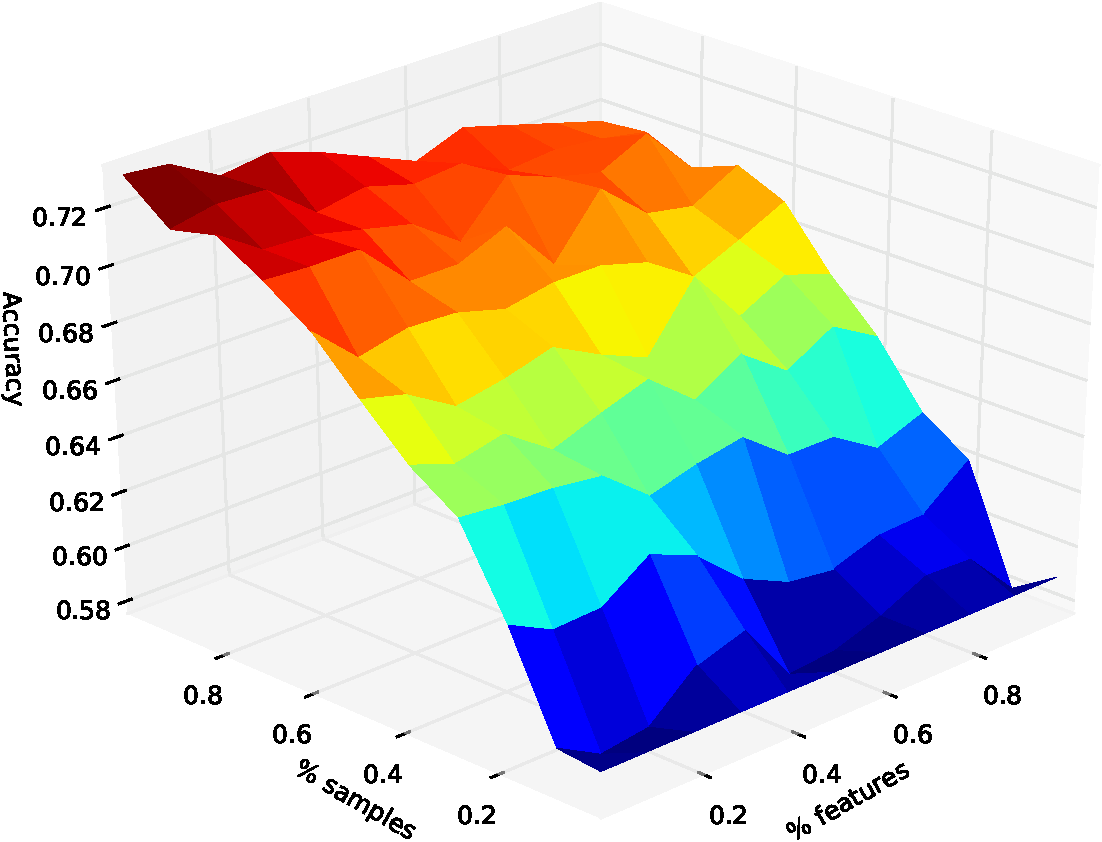
\includegraphics[width=0.31\textwidth]{figures/ch8/figure3-a-arcene-rp-et.pdf}
        }
        \subfloat[\textsc{cifar10} (RP-ET)]{
            \label{fig:surfaces:cifar10}
            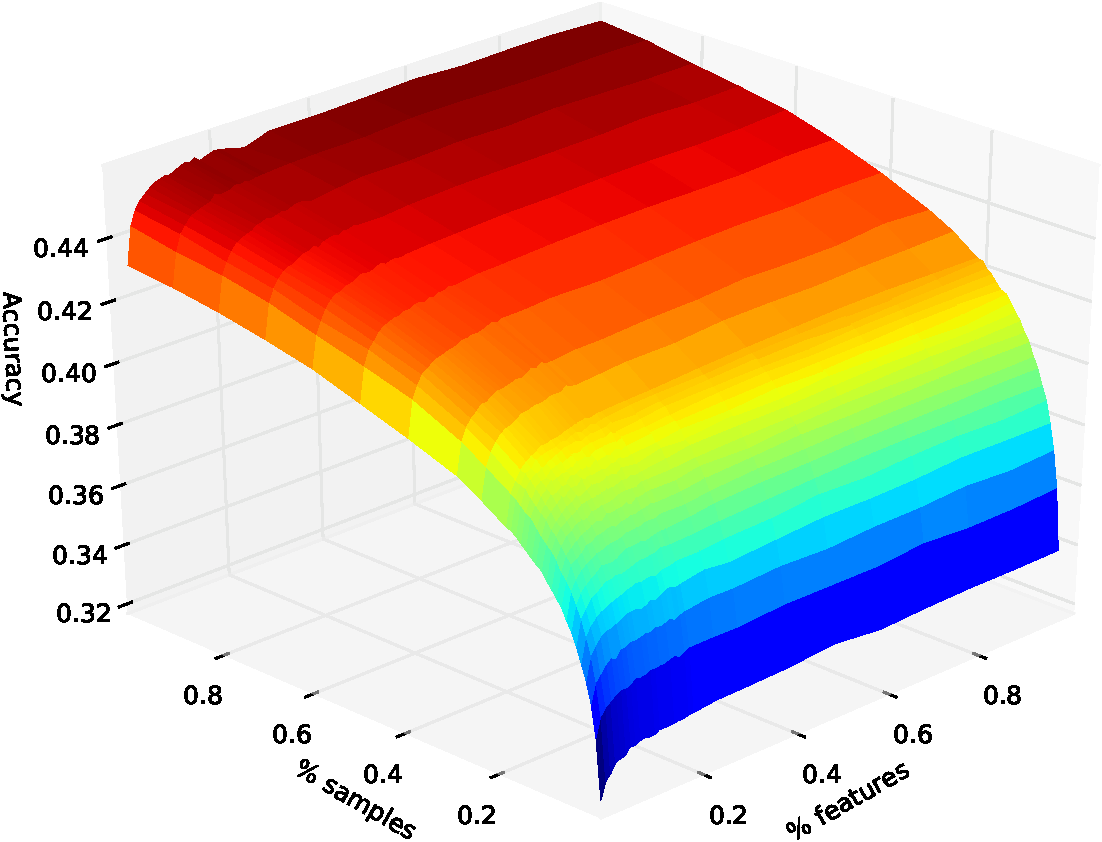
\includegraphics[width=0.31\textwidth]{figures/ch8/figure3-b-cifar10-rp-et.pdf}
        }
        \subfloat[\textsc{tis} (RP-ET)]{
            \label{fig:surfaces:tis}
            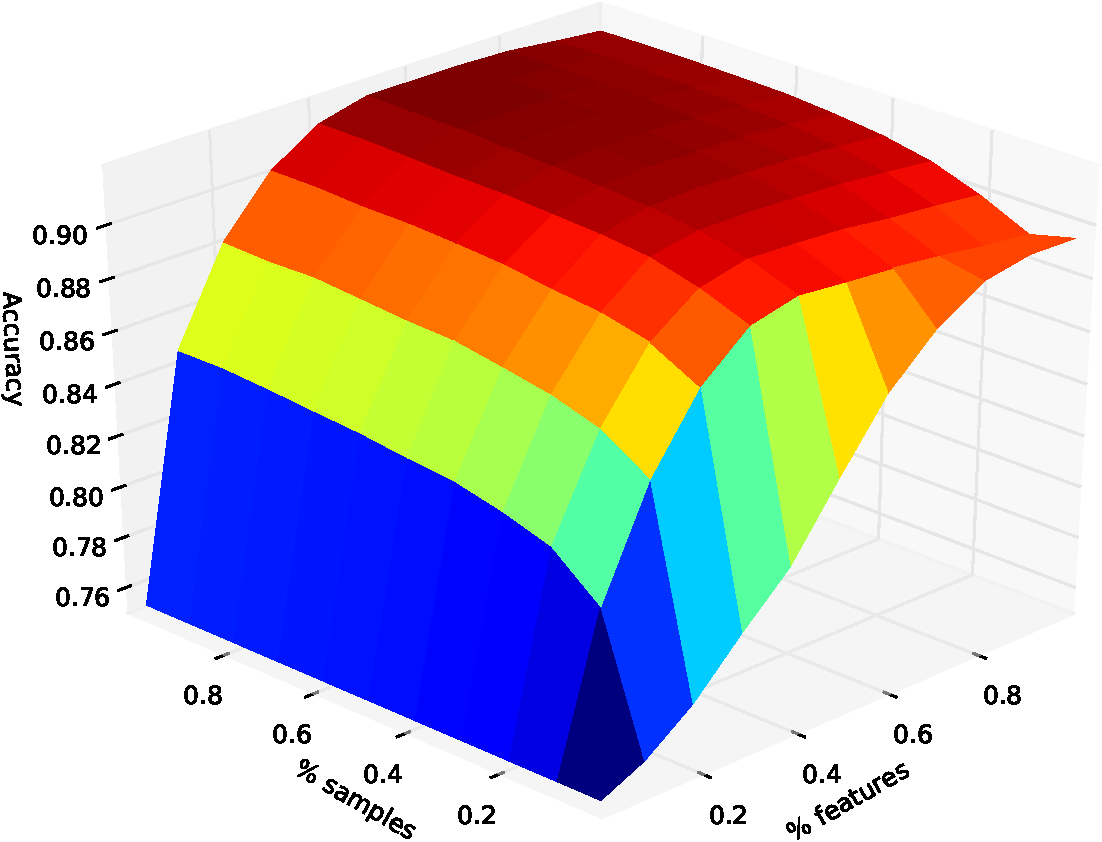
\includegraphics[width=0.31\textwidth]{figures/ch8/figure3-c-tis-rp-et.pdf}
        }

        \setcounter{subfigure}{0}
        \subfloat[\textsc{arcene} (RP-DT)]{
            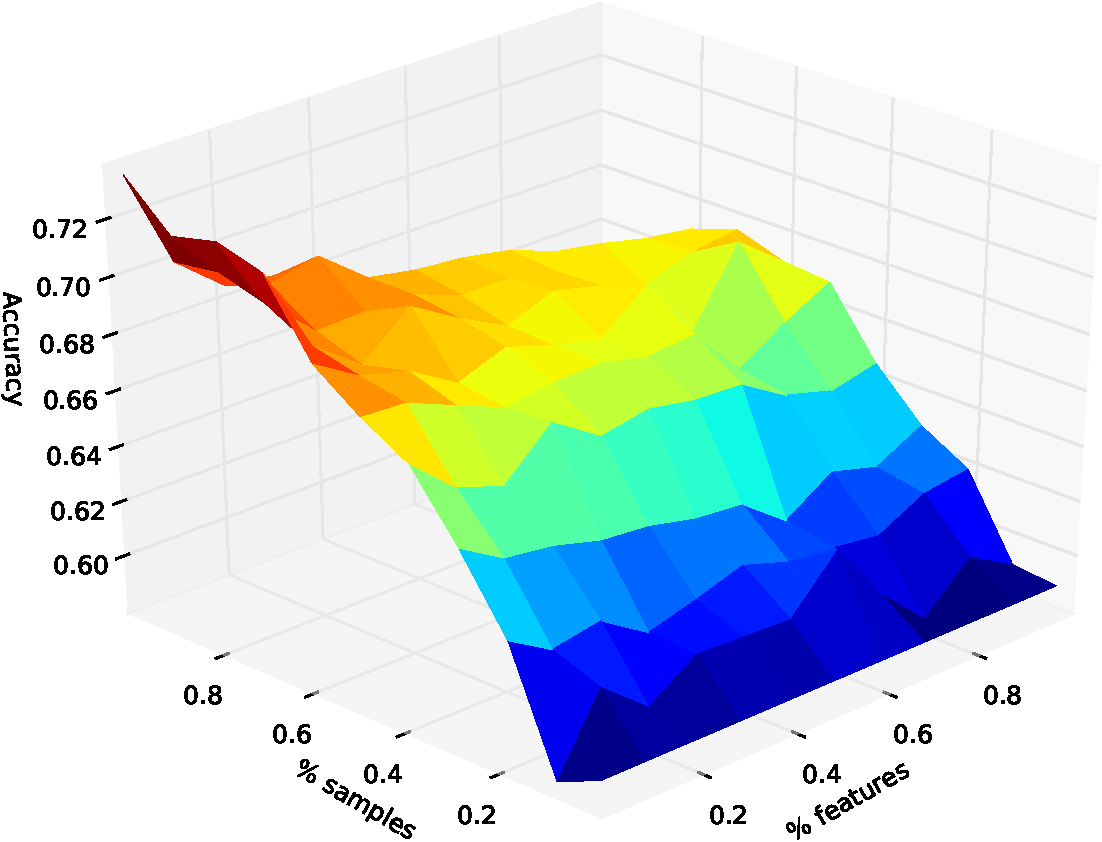
\includegraphics[width=0.31\textwidth]{figures/ch8/figure3-a-arcene-rp-dt.pdf}
        }
        \subfloat[\textsc{cifar10} (RP-DT)]{
            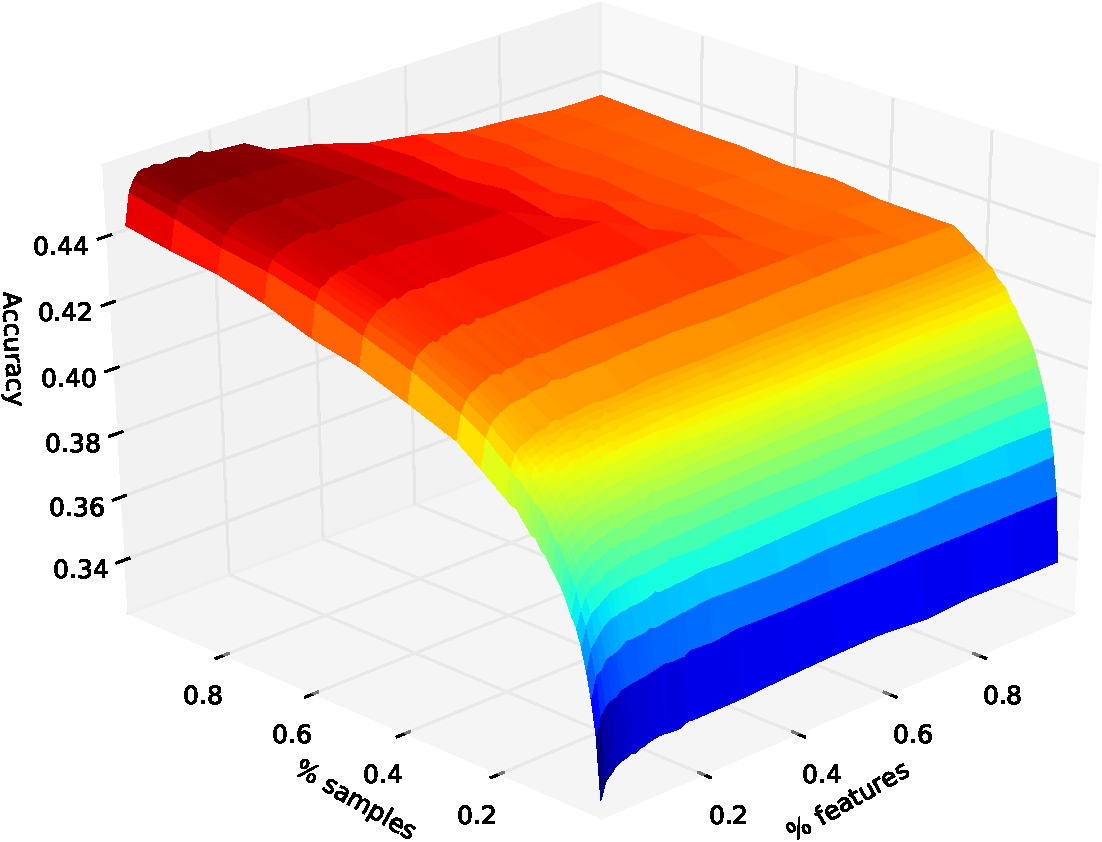
\includegraphics[width=0.31\textwidth]{figures/ch8/figure3-b-cifar10-rp-dt.pdf}
        }
        \subfloat[\textsc{tis} (RP-DT)]{
            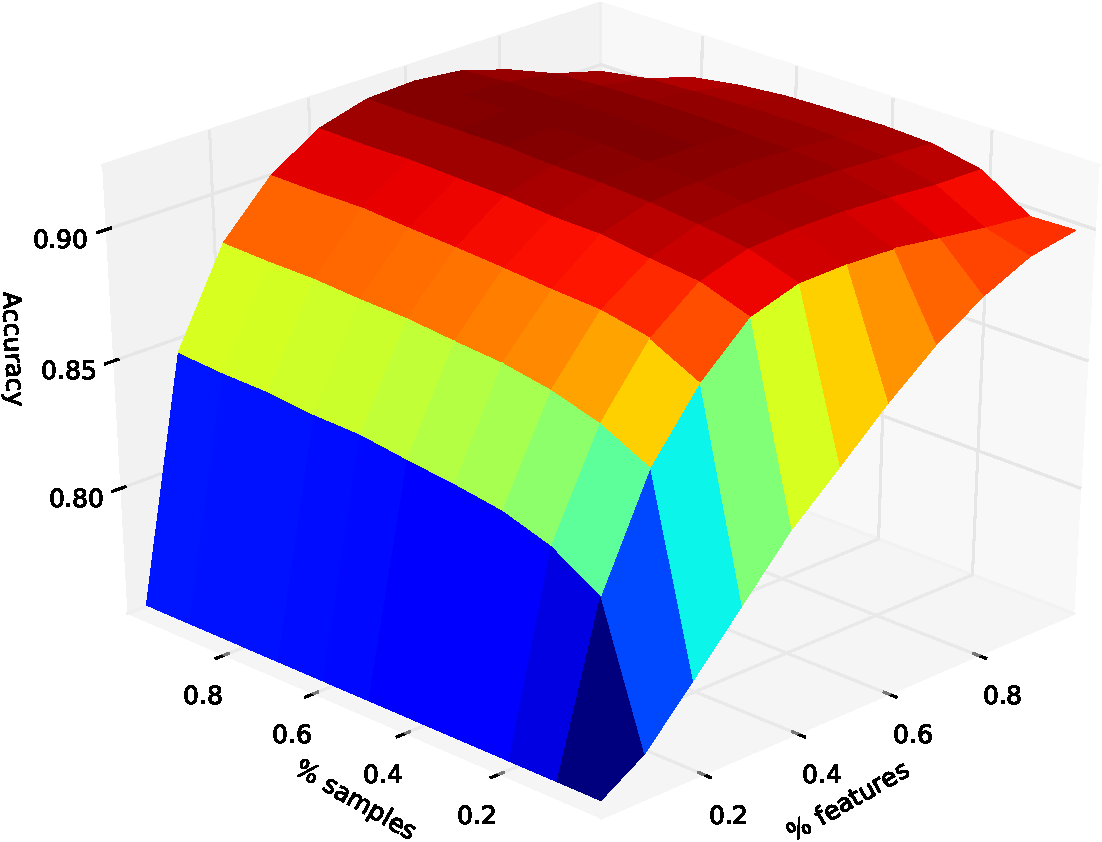
\includegraphics[width=0.31\textwidth]{figures/ch8/figure3-c-tis-rp-dt.pdf}
        }


        \subfloat[\textsc{madelon} (RP-ET)]{
            \label{fig:surfaces:madelon}
            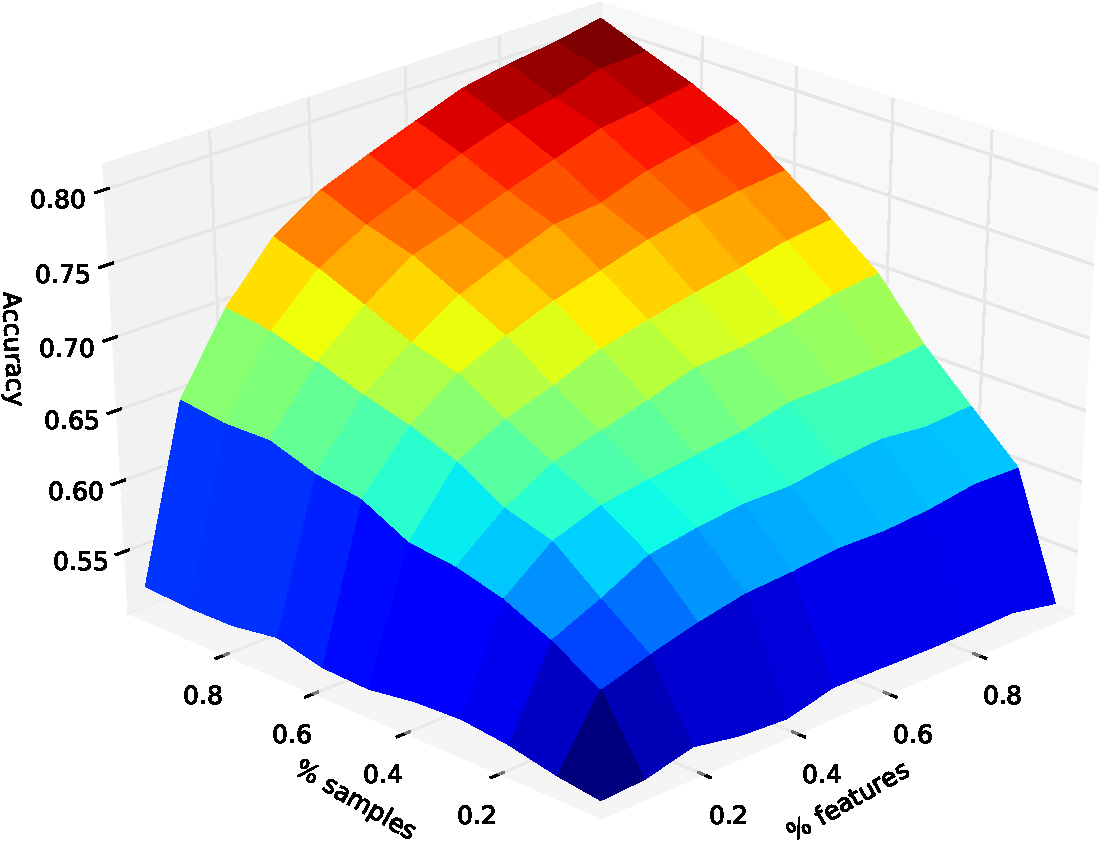
\includegraphics[width=0.31\textwidth]{figures/ch8/figure3-d-madelon-rp-et.pdf}
        }
        \subfloat[\textsc{isolet} (RP-ET)]{
            \label{fig:surfaces:isolet}
            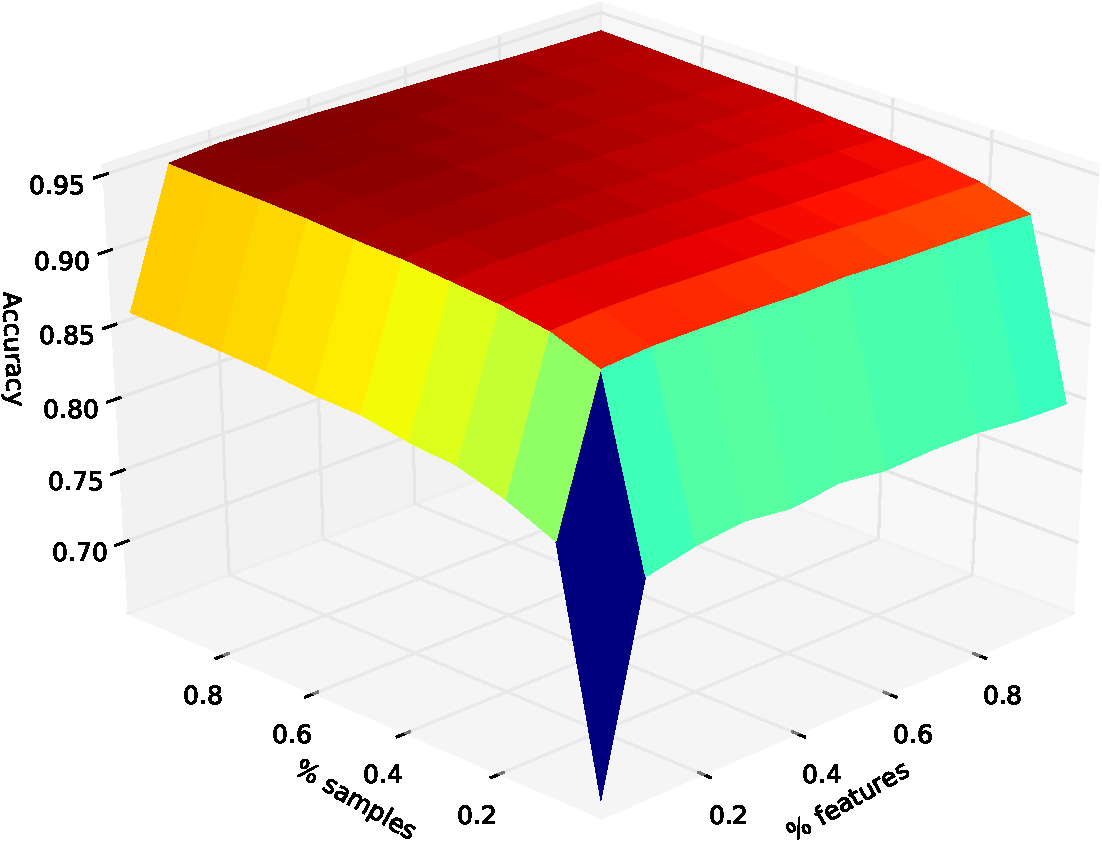
\includegraphics[width=0.31\textwidth]{figures/ch8/figure3-e-isolet-rp-et.pdf}
        }
        \subfloat[\textsc{mnist3vs8} (RP-ET)]{
            \label{fig:surfaces:mnist}
            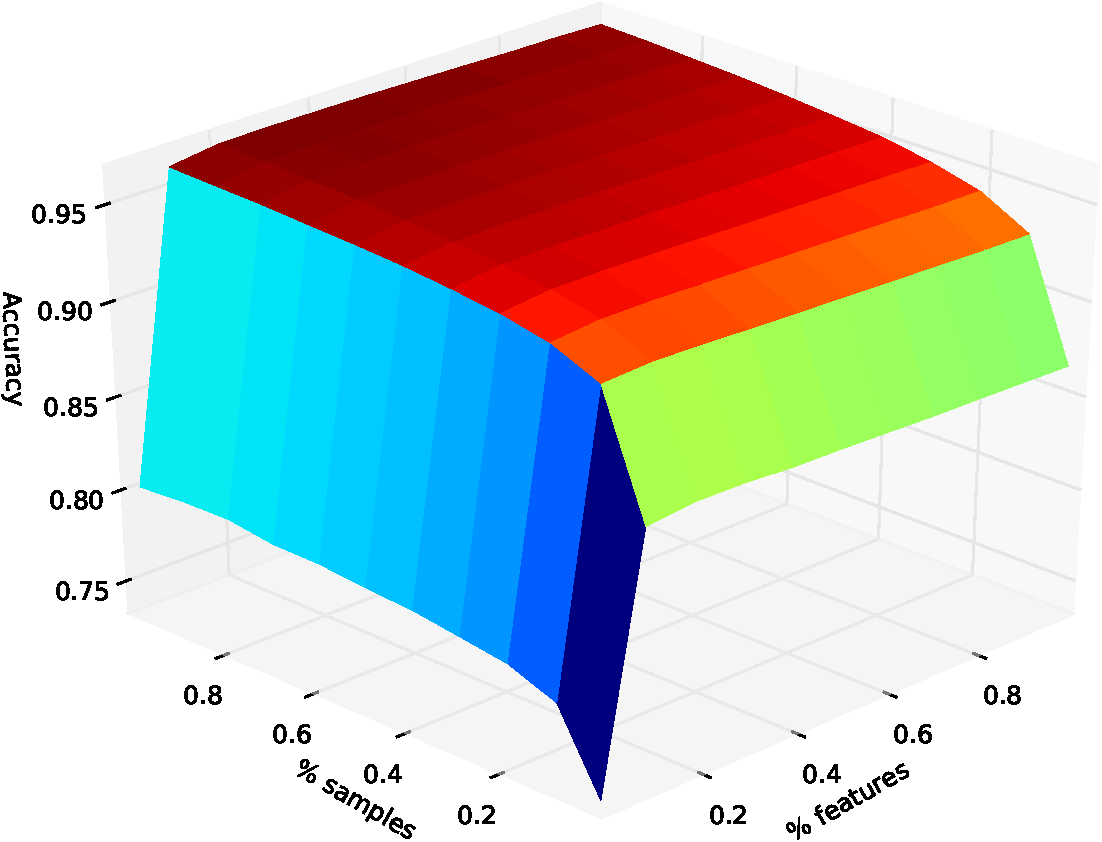
\includegraphics[width=0.31\textwidth]{figures/ch8/figure3-f-mnist-rp-et.pdf}
        }

        \setcounter{subfigure}{3}
        \subfloat[\textsc{madelon} (RP-DT)]{
            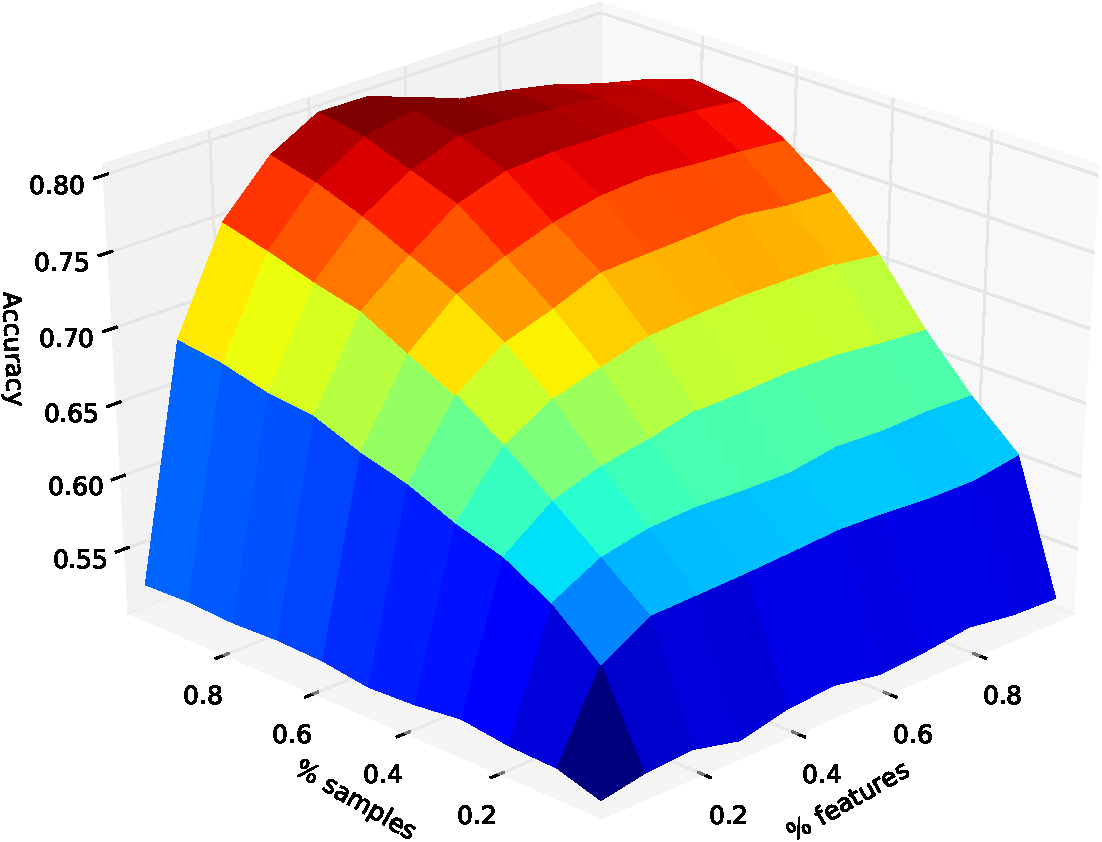
\includegraphics[width=0.31\textwidth]{figures/ch8/figure3-d-madelon-rp-dt.pdf}
        }
        \subfloat[\textsc{isolet} (RP-DT)]{
            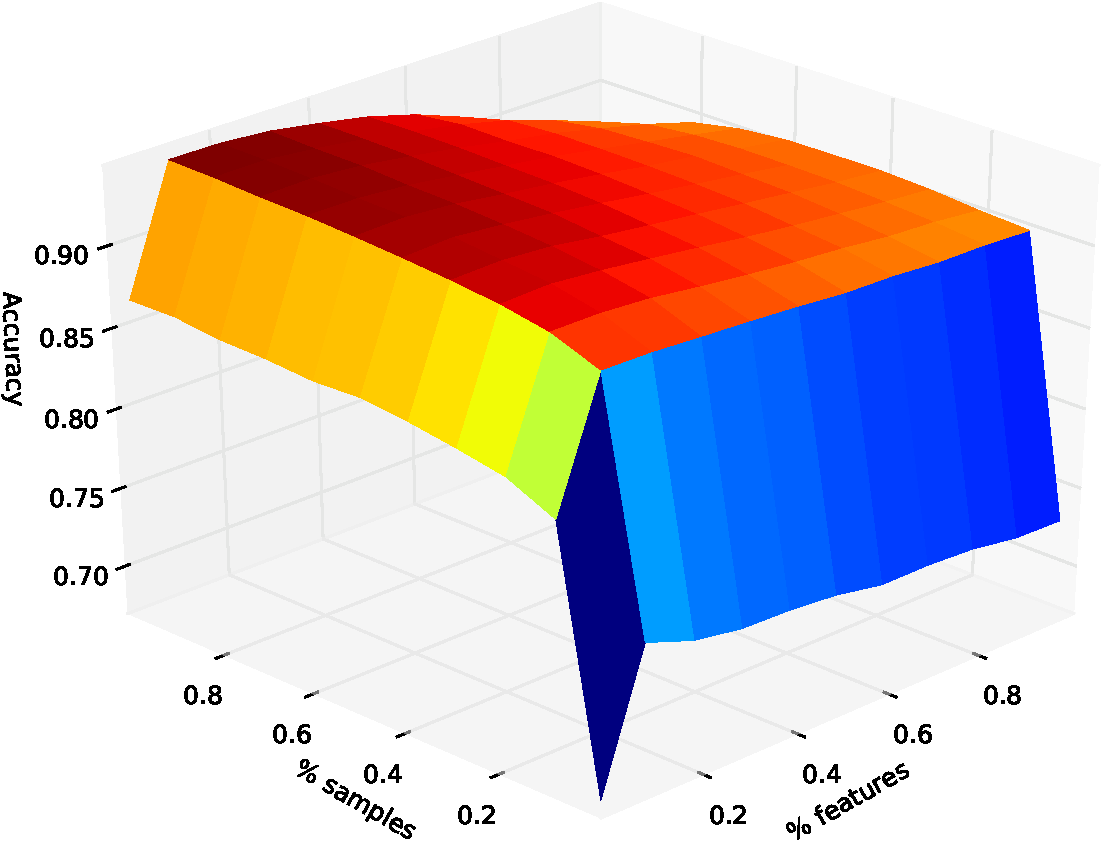
\includegraphics[width=0.31\textwidth]{figures/ch8/figure3-e-isolet-rp-dt.pdf}
        }
        \subfloat[\textsc{mnist3vs8} (RP-DT)]{
            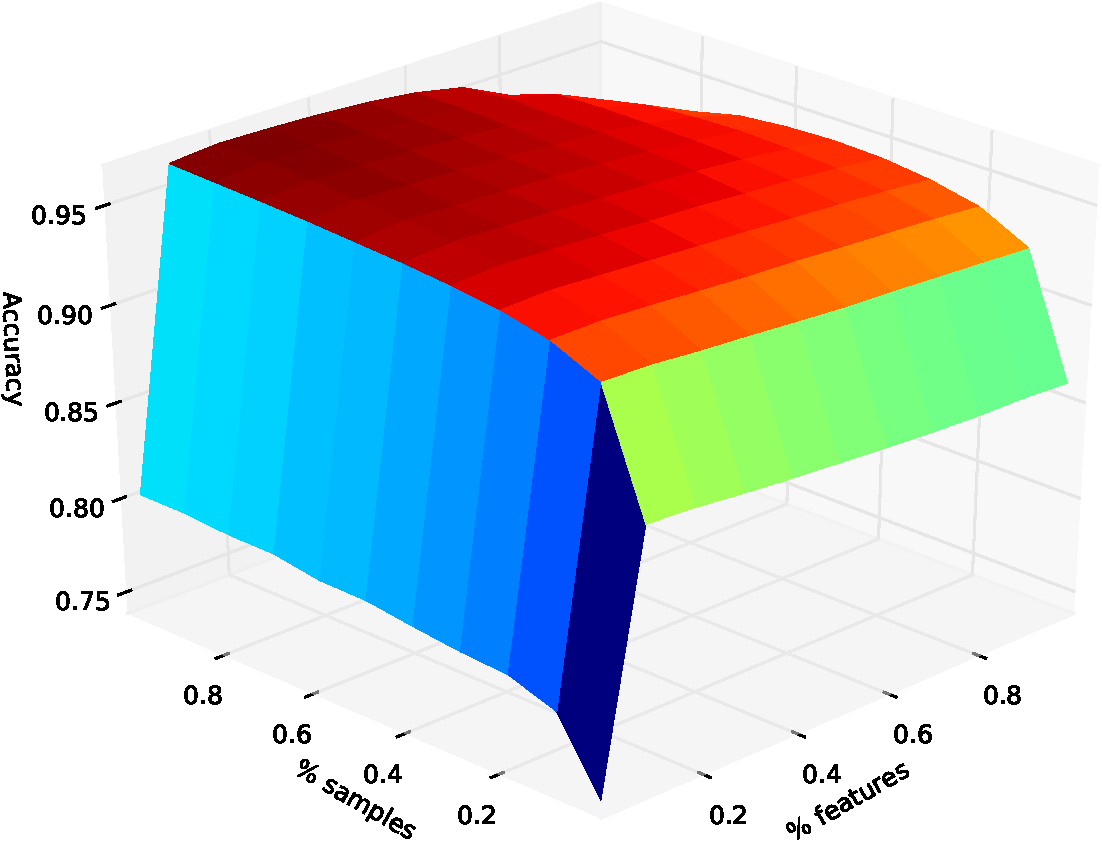
\includegraphics[width=0.31\textwidth]{figures/ch8/figure3-f-mnist-rp-dt.pdf}
        }
\caption{Learning surfaces.}
\label{fig:9:surfaces}
\end{center}
\end{figure}

The choice of the base estimators does not have a strong impact on the aspect
of the curves (compare the 1$^{st}$ and 3$^{rd}$ rows of sub-figures in
Figure~\ref{fig:9:surfaces} with those in the 2$^{nd}$ and 4$^{th}$ rows). The only
difference is the decrease of the accuracy of RP-DT when $\alpha_s$ and
$\alpha_f$ grow towards $1.0$. Indeed, since the only source of randomization in RP-DT
is patch selection, it yields in this case ensembles of identical
trees and therefore amounts to build a single tree on the whole
dataset. By contrast, because of the extra-randomization of the split
thresholds in ET, there is typically no drop of accuracy for RP-ET when $\alpha_s$
and $\alpha_f$ grow to $1.0$.

Overall, this analysis suggests that not only the best pair $\alpha_s \alpha_f$ depends
on the problem, but also that the sensitivity of the ensemble to changes to the
size of a random patch is both problem and base estimator specific. As a
result, these observations advocate for a method that could
favor $\alpha_s$, $\alpha_f$ or both, and do so
appropriately given the base estimator.

\subsection{Memory reduction, without significant loss}
\label{sec:9:memory:noloss}

We proceed to study in this section the actual size of the random patches when
the values of $\alpha_s$ and $\alpha_f$ are tuned using an independent validation
set. Our results are summarized in Figure~\ref{fig:9:memory:original}. Each
ellipse corresponds to one of the 29 datasets of our benchmark, whose center is
located at $(\overline{\alpha_s}, \overline{\alpha_f})$ (i.e., the average parameter
values over the 50 runs) and whose semi-axes correspond to the standard
deviations of $\alpha_s$ and $\alpha_f$. Any point in the plot corresponds to a pair
$(\alpha_s, \alpha_f)$ and thus to a relative consumption $\mu' = \alpha_s \alpha_f$ of memory. To
ease readability, level curves are plotted for $\mu' = 0.01, 0.1, ..., 0.9$. In
the right part of the figure, the histogram counts the number of datasets such
that $\overline{\alpha_s}\cdot\overline{\alpha_f}$ falls in the corresponding level set.

Figure~\ref{fig:9:memory:original} corroborates our previous discussion. On some
datasets, it is better to favor $\alpha_s$ while on some other increasing $\alpha_f$ is
a better strategy. The various sizes of the ellipses also confirm that the
sensitivity to variations of $\alpha_s$ and $\alpha_f$ is indeed problem-specific. The
figure also clearly highlights the fact that, even under no memory constraint, the
optimal patches rarely consume the whole memory. A majority of ellipses indeed
lie below the level set $\mu'=0.5$ and only a couple of them are above
$\mu'=0.75$. With respect to ET or RF for which the base estimators are all built
on the whole dataset, this means that ensembles of patches are not only as
competitive but also less memory greedy. In addition, the figure also
points out the difference between RP-ET and RP-DT as discussed in the previous
section. To ensure diversity, RP-DT is constrained to use smaller patches than
RP-ET, hence explaining why the ellipses in red are on average below those in
blue. While RP-DT proved to be a bit less competitive in terms of accuracy,
this indicates on the other hand that RP-DT may actually be more interesting
from a memory consumption point of view.

\begin{figure}
\begin{center}
        \subfloat[Original patches]{
            \label{fig:9:memory:original}
            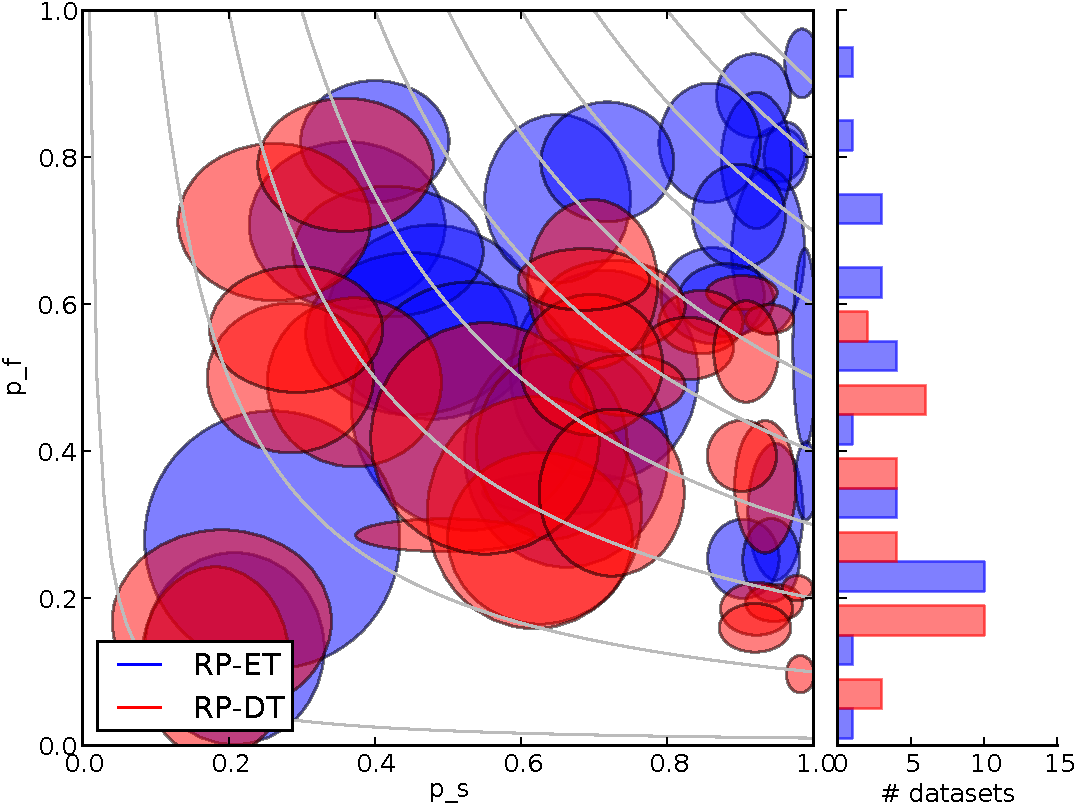
\includegraphics[width=0.5\textwidth]{figures/ch8/figure4-none.pdf}
        }
        \subfloat[Reduced patches]{
            \label{fig:9:memory:opt}
            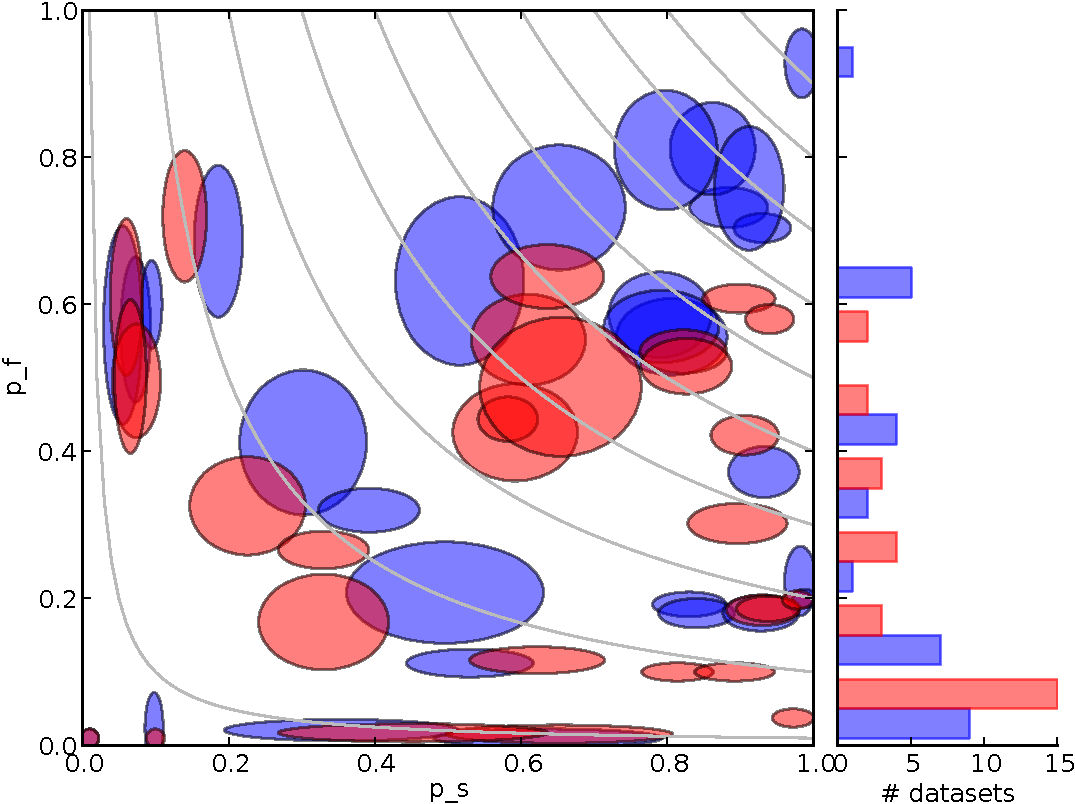
\includegraphics[width=0.5\textwidth]{figures/ch8/figure4-mem.pdf}
        }
\caption{Optimal sizes of the random patches on our benchmark.}
\label{fig:9:memory}
\end{center}
\end{figure}

In Section~\ref{sec:9:memory:sensitivity}, we observed plateaus or very
gentle slopes around the optimal pair $(\alpha_s, \alpha_f)$.  From a memory point of
view, this suggests that the random patches are likely to be reducible without
actually degrading the accuracy of the resulting ensemble. Put otherwise, our
interest is to find the smallest size $\alpha_s \alpha_f$ such that the accuracy of the
resulting ensemble is not significantly worse than an ensemble built without
such constraint. To that end, we study the extent at which the constraint $\alpha_s
\alpha_f < \mu'_{\text{max}}$ can be strengthened without any significant drop in
accuracy. If $\mu'_{\text{max}}$ can be reduced significantly then it would indeed mean that
even when only small parts of the data are actually used to build single base
estimators, competitive performance can still be achieved.

Figure~\ref{fig:9:memory:opt} summarizes our results. For all datasets, $\mu'_{\text{max}}$
was set to the lowest value such that it cannot be statistically detected that
the average accuracy of the resulting ensemble is different from the average
accuracy of an ensemble built with no memory constraint (at $\alpha=0.05$). With
regard to Figure~\ref{fig:9:memory:original}, the shift of most ellipses to lower
memory level sets confirm our first intuition. In many cases, the size of the
random patches can indeed be reduced, often drastically, without significant
decrease of accuracy. For more than half of the datasets, memory can indeed be
decreased to $\mu'=0.1$ or $\mu'=0.2$. In other words, building trees on small parts
of the data (i.e., $10\%$ or $20\%$ of the original dataset) is, for more than
half of the datasets, enough to reach competitive accuracy. Also, the
sensitivity to $\alpha_s$ and $\alpha_f$ is now even more patent. Some ensembles use very
few samples ($\alpha_s < 0.1$) but with many features, while other uses many samples
with few features ($\alpha_f < 0.1$). Again, from a memory point of view, RP-DT
appears to be more interesting than RP-ET. The memory reduction is larger, as
the histogram indicates. Optimized splits in the decision trees may indeed lead
to a better exploitation of the data, hence to a potentially larger reduction of
memory. In conclusion, while not detecting significant differences in accuracy
does not allow to conclude that the performances are truly similar, these
figures at least illustrate that memory requirements can be drastically reduced
without apparent loss in accuracy.

\subsection{Memory reduction, with loss}
\label{sec:9:memory:loss}

The previous section has shown that the memory consumption can be reduced up to
some threshold $\mu'_{\text{max}}$ with no significant loss in accuracy. In this section we
now look at the accuracy of the resulting ensemble when $\mu'_{\text{max}}$ is further
decreased. We argue that with severe constraints, and because datasets have all a
different sensitivity, it is even more crucial to better exploit data and thus
to find the right trade-off between both $\alpha_s$ and $\alpha_f$, as only RP can.

\begin{figure}
\begin{center}
        \subfloat[\textsc{arcene}]{
        \label{fig:memc:arcene}
            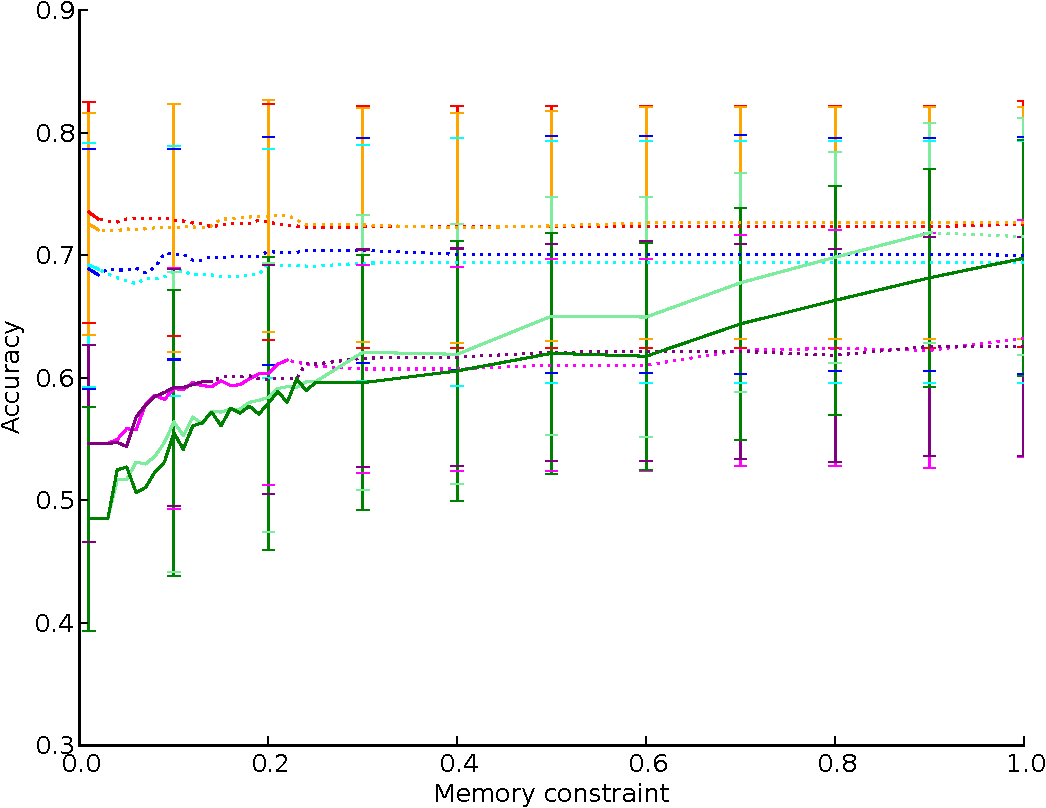
\includegraphics[width=0.5\textwidth]{figures/ch8/figure5-a-arcene.pdf}
        }
        \subfloat[\textsc{cifar10}]{
        \label{fig:memc:cifar10}
            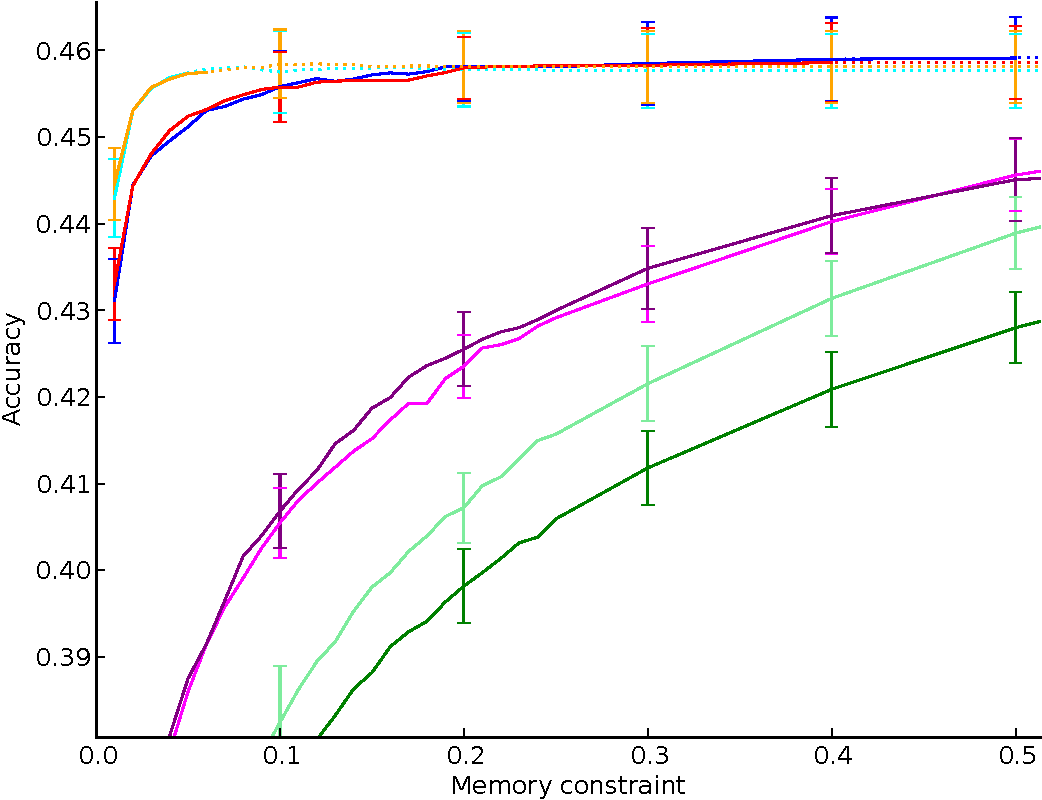
\includegraphics[width=0.5\textwidth]{figures/ch8/figure5-b-cifar10.pdf}
        }

        \subfloat[\textsc{tis}]{
        \label{fig:memc:tis}
            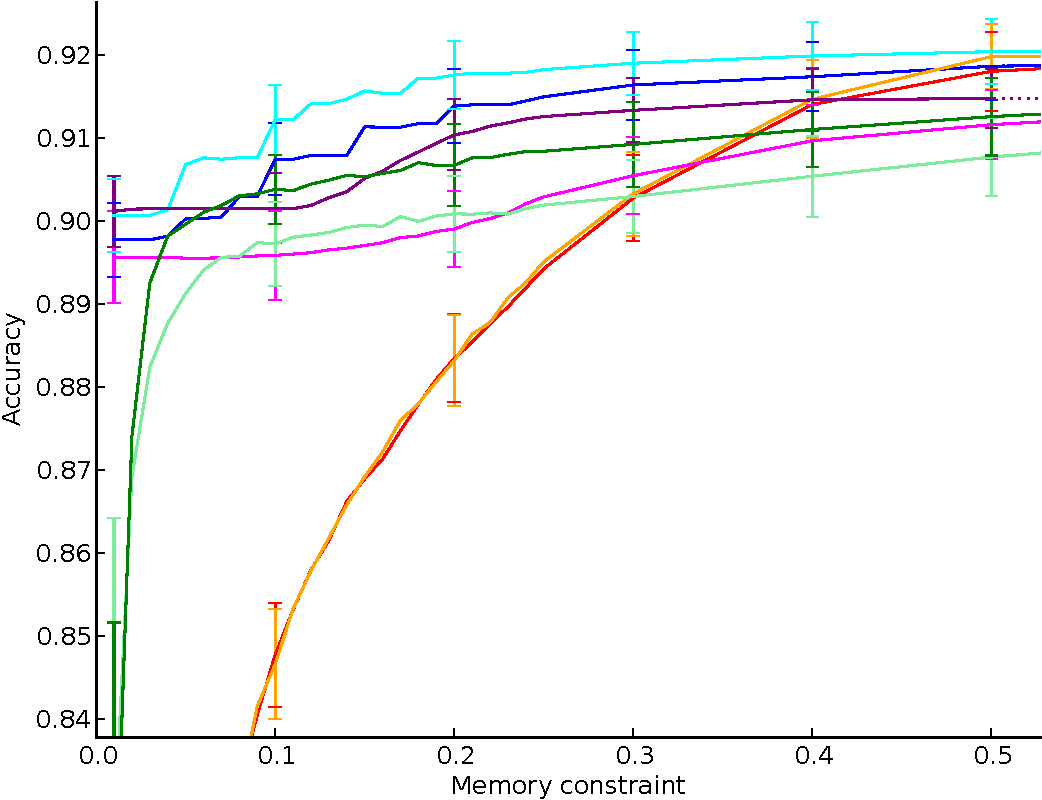
\includegraphics[width=0.5\textwidth]{figures/ch8/figure5-c-tis.pdf}
        }
        \subfloat[\textsc{madelon}]{
        \label{fig:memc:madelon}
            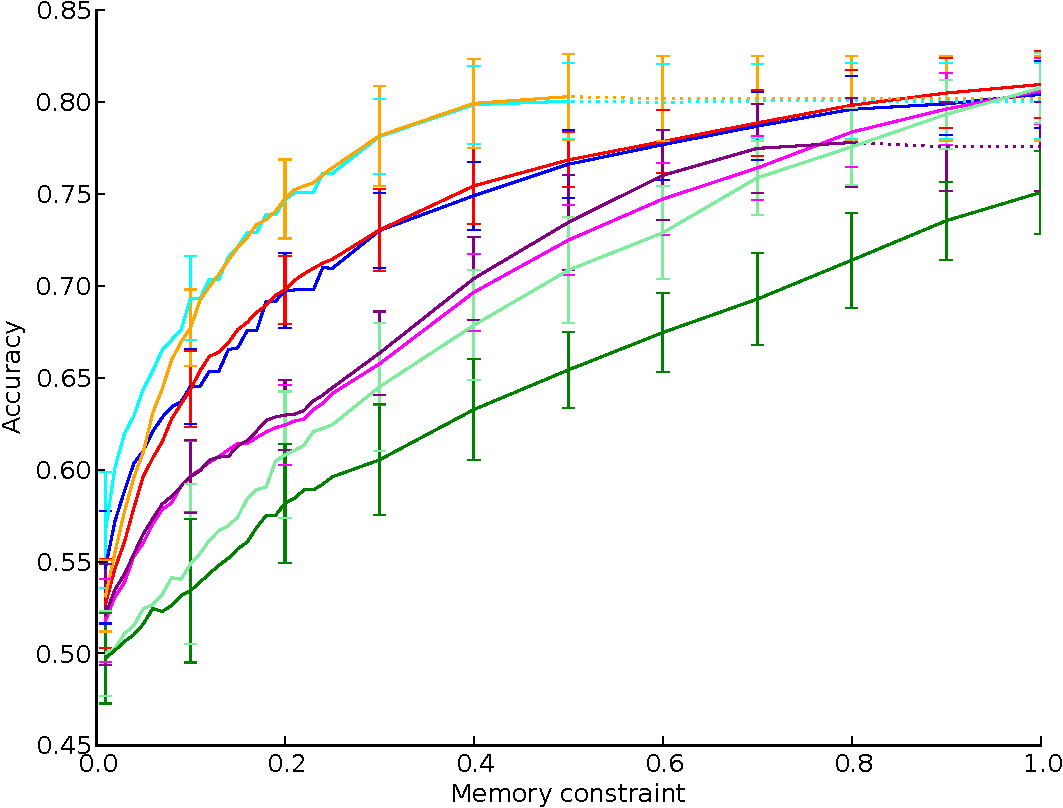
\includegraphics[width=0.5\textwidth]{figures/ch8/figure5-d-madelon.pdf}
        }

        \subfloat[\textsc{isolet}]{
        \label{fig:memc:isolet}
            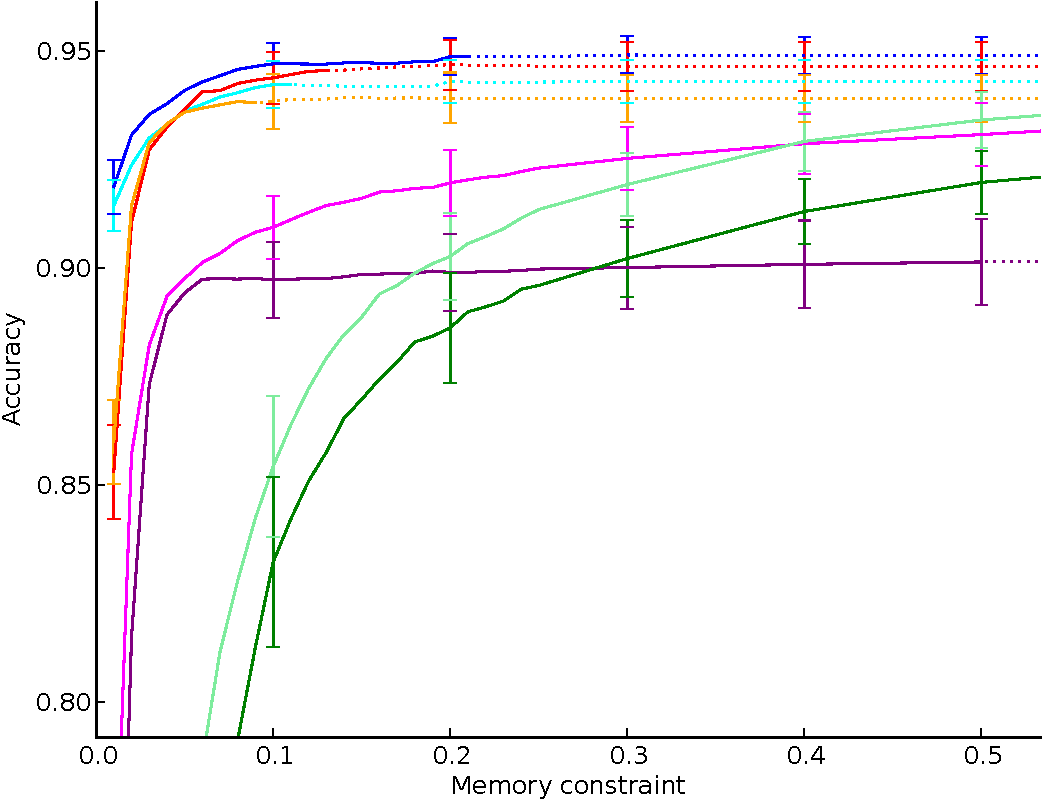
\includegraphics[width=0.5\textwidth]{figures/ch8/figure5-e-isolet.pdf}
        }
        \subfloat[\textsc{mnist3vs8}]{
        \label{fig:memc:mnist}
            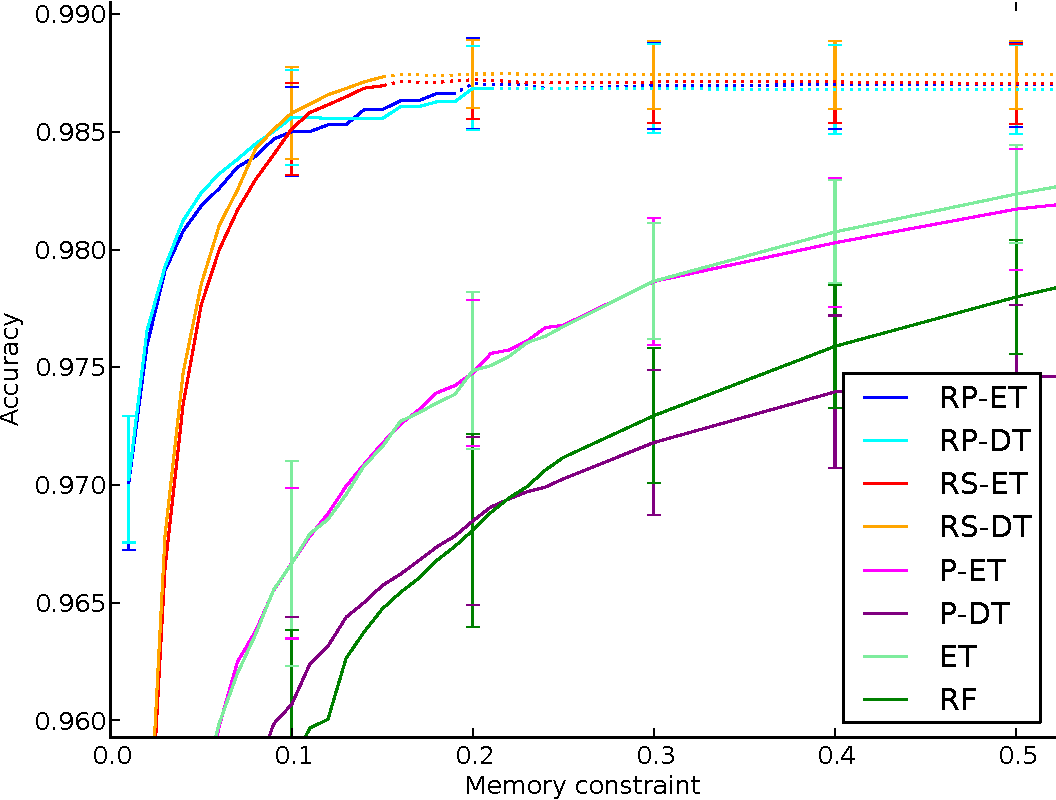
\includegraphics[width=0.5\textwidth]{figures/ch8/figure5-f-mnist.pdf}
        }
\caption{Accuracy under memory constraint.}
\label{fig:9:memc}
\end{center}
\end{figure}

To illustrate our point, Figure~\ref{fig:9:memc} compares for 6 representative
datasets the accuracy of the methods with respect to the memory constraint $\alpha_s
\alpha_f < \mu'_{\text{max}}$.  A plain line indicates that the generalization error of the
best resulting ensemble under memory constraint $\mu'_{\text{max}}$ is significantly (at $\alpha=0.05$)
worse on the test sets than when there is no constraint
(i.e., $\mu'_{\text{max}}=1$). A dotted line indicates that on average, on the test set, the
ensemble is not significantly less accurate.

As the figure shows, when $\mu'_{\text{max}}$ is low, RP-based ensembles often achieve
the best accuracy. Only on \textsc{arcene} (Figure~\ref{fig:memc:arcene}), RS seems to be a
better strategy, suggesting some overfitting in setting $\alpha_s$ in RP. On all 5
other example datasets, RP is equivalent or better than RS and P for low values
of $\mu'_{\text{max}}$, with the largest gaps appearing on \textsc{isolet}
(Figure~\ref{fig:memc:isolet}) and \textsc{mnist3vs8} (Figure~\ref{fig:memc:mnist}). As
already observed in the previous section, although RP-DT is not the best
strategy when memory is unconstrained, its curve dominates the curve of RP-ET
for small values of $\mu'_{\text{max}}$ in Figures \ref{fig:memc:cifar10},
\ref{fig:memc:tis}, and \ref{fig:memc:madelon}. Because split thresholds are
not randomized in RP-DT, this method is more resistant than RP-ET to the strong
randomization induced by a very low $\mu'_{\text{max}}$ threshold.

For comparison, Figure~\ref{fig:9:memc} also features the learning curves of both
ET and RF (with $K$ optimized on the validation set), in which the trees have
all been built on the {\it same} training sample of $\mu'_{\text{max}}N$ instances,
with all features. These results are representative of the use of a
straightforward sub-sampling of the instances to handle the memory constraint.
On all datasets, this setting yields very poor performance when $\mu'_{\text{max}}$ is
low. Building base estimators on re-sampled random patches thus brings a clear advantage to RP, RS and P and hence confirms the conclusions of \citet{basilico:2011} who showed that using more data indeed produces
more accurate models than learning from a single sub-sample.
This
latter experiment furthermore shows that the good performances of RP
cannot be trivially attributed to the fact that our datasets contain so many
instances that only processing a sub-sample of them would be enough. On most
problems, the slopes of the learning curves of RF and ET indeed suggest that
convergence has not yet been reached on these datasets. Yet, important
improvement are gained by sub-sampling random patches.
Contrary to intuition, it
also does not appear that the bigger the datasets, the lower $\mu'_{\text{max}}$ can be
reduced without loss of accuracy. Indeed, we found no conclusive correlation
between the size $Np$ of the dataset and the minimum value of $\mu'_{\text{max}}$ to
reach good performance\footnote{Spearman's rank correlation coefficient is
-0.0354 ($p-\mathrm{value}=0.8550$).}.
Overall, these results thus indicate that
building an ensemble on random patches is not only a good strategy when data is
abundant and redundant but also that it works even for scarce datasets with
limited information regarding the problem.

\subsection{Conclusions}

We have shown in this section that the memory requirements of sampling-based
ensembles are intrinsically low. Better, we have shown that they can often be
drastically decreased without significant loss in accuracy. When the size of the
dataset is far bigger than the available memory, we have also demonstrated that
sampling data along both samples and features, as RP does, not only competes
with other ensemble algorithms but also significantly improves the accuracy of
the resulting ensemble. It also brings a significant improvement over a
straightforward sub-sampling of the instances.

\section{Overall conclusions}
\label{sec:9:conclusions}

The main contribution of this work is to explore a new framework for supervised
learning in the context of very strong memory constraints or, equivalently, very
large datasets. To address such problems, we proposed the Random Patches
ensemble method that builds each individual model of the ensemble from a random
patch of the dataset obtained by drawing random subsets of both samples and
features from the whole dataset. Through extensive experiments with tree-based
estimators, we have shown that this strategy works as well as other popular
randomization schemes in terms of accuracy (Section~\ref{sec:9:accuracy}), at the
same time reduces very significantly the memory requirements to build each
individual model (Section~\ref{sec:9:memory:noloss}), and, given its flexibility,
attains significantly better accuracy than other methods when memory is severely
constrained (Section~\ref{sec:9:memory:loss}). Since all models are built
independently of each other, the approach is furthermore trivial to parallelize.
All in all, we believe that the paradigm of our method highlights a very promising
direction of research to address supervised learning on big data.

There remain several open questions and limitations to our approach that we
would like to address in the future. First, this study motivates our interest in
experimenting with truly large-scale problems (of giga-scale and higher). Since
RP already appears advantageous for small to medium datasets, the potential benefits on
very large-scale data indeed look very promising.

Second, the conclusions drawn in sections~\ref{sec:9:accuracy} and
\ref{sec:9:memory} are all based on the optimal values of the parameters $\alpha_s$ and
$\alpha_f$ tuned through an exhaustive grid search on the validation set. Our
analysis did not account for the memory and time required for tuning these two
parameters. In practice, hyper-parameter tuning can not be avoided as we have
shown that the optimal trade-off between $\alpha_f$ and $\alpha_s$ was problem dependent.
It would therefore be interesting to design an efficient strategy to
automatically find and adjust the values of $\alpha_s$ and $\alpha_f$, taking into account
the global memory constraint. Our simplistic framework also only accounts for
the memory required to store the training set in memory and not for the total
memory required to actually build the ensemble.

We have only explored uniform sampling of patches of fixed size in our
experiments. In the context of the Pasting approach, Breiman proposed
an iterative instance weighting scheme that proved to be more
efficient than uniform sampling \citep{breiman:1999}. It would be
interesting to extend this approach when sampling both instances and
features. Yet, parallelization would not be trivial anymore, although
probably still possible in the line of the work in \citep{chawla:2004}.

Finally, our analysis of RP is
mostly empirical. In the future, we would like to strengthen these
results with a more theoretical analysis. A starting point could be
the work in \citep{zinkevich:2010} that studies a scheme similar to the
Pasting method applied to linear models trained through parallel
stochastic gradient descent. The extension of this work to non
parametric tree-based estimators does not appear trivial however,
since these latter are not well characterized
theoretically.



% Back pages ==================================================================
\appendix
\cleardoublepage
\part{Appendix}

\cleardoublepage%********************************************************************
% Bibliography
%*******************************************************
% work-around to have small caps also here in the headline
\manualmark
\markboth{\spacedlowsmallcaps{\bibname}}{\spacedlowsmallcaps{\bibname}} % work-around to have small caps also
%\phantomsection 
\refstepcounter{dummy}
\addtocontents{toc}{\protect\vspace{\beforebibskip}} % to have the bib a bit from the rest in the toc
\addcontentsline{toc}{chapter}{\tocEntry{\bibname}}
\bibliographystyle{plainnat}
\label{app:bibliography} 
\bibliography{Bibliography}

\end{document}
